\documentclass[11pt]{book}
%%%%%%%%%%%%%%%%%%%%%%%%%%%%%
% Ancienne version
%\usepackage[latin1]{inputenc}% pour les accents
%\usepackage[scale=.85]{geometry}
%\usepackage[french]{babel}
%%%%%%%%%%%%%%%%%%%%%%%%%%%%%
% Nouvelle version pour les accents
\usepackage[T1]{fontenc}
\usepackage[utf8]{inputenc}
\usepackage[french]{babel}
\usepackage{textcomp}
% \usepackage{siunitx}
\usepackage[scale = .85]{geometry}
%	\setlength{\textwidth}{159.8mm} 
%	\setlength{\oddsidemargin}{6.6mm}
%	\setlength{\evensidemargin}{0.8mm}
%	\setlength{\topmargin}{-15.2mm} 
%	\setlength{\textheight}{238.9mm}
	\setlength{\headheight}{14pt}
%	\setlength{\parindent}{0pt}

\usepackage{setspace} % increase interline spacing slightly
	\setstretch{1.1}
\usepackage{parskip}
	\setlength{\parskip}{2cm}
%%%%%%%%%%%%%%%%%%%%%%%%%%%%%

\frenchbsetup{StandardLists=true} % pour eviter les conflits entre babel et enumitem
\usepackage{makeidx, xcolor}
\usepackage[colorlinks]{hyperref}   % choisir pour la version pdf
\hypersetup{linkcolor=blue,urlcolor=blue}
%\usepackage{hyperref}    % choisir pour l'impression (noir et blanc)
\usepackage{amsmath}
%\uspackage{amssymb,amsmath,amsfonts,mathptmx}
\usepackage{eurosym}
\usepackage{wrapfig, pifont, fancybox, fancyhdr, multicol, enumitem, subfig, booktabs}
\usepackage{graphicx}
\graphicspath{{../Images/}}

%\renewcommand{\chaptermark}[1]{\bsc{\chaptername~\thechapter{} : #1}}
\pagestyle{fancy}
\fancyhead{}
\fancyhead[RO,LE]{\thepage}
\fancyhead[RE]{\leftmark}
\fancyhead[LO]{\rightmark}
\fancyfoot{}
\renewcommand{\headrulewidth}{0.4pt}
\renewcommand{\footrulewidth}{0.pt}

% Commandes utiles
\usepackage{xspace}
\newcommand*{\MCF}{MCF\xspace}
\newcommand*{\PR}{PR\xspace}


\newcommand {\lien}[1]{{\small\tt \href{http\string://#1}{http\string://#1}}}
\newcommand {\liens}[1]{{\small\tt \href{https\string://#1}{https\string://#1}}}
\newcommand {\lienftp}[1]{{\small\tt \href{ftp\string://#1}{http\string://#1}}}
\makeindex

%%%%%%%%%%%%%%
% La commande ci-dessous ne fait rien mais permet par un simple ctrl+F de retrouver rapidement les
% informations a verifier a chaque nouvelle edition (noms des directeur.trices par exemple).
%%%%%%%%%%%%%%

\newcommand{\verifier}[1]{\textcolor{black}{#1}}



\begin{document}
\renewcommand{\labelitemi}{$\bullet$}
\setlist{noitemsep,nosep}
\setlength{\parindent}{0cm}

{\pagestyle{empty}
%
~\hfill
\includegraphics[height=1.25cm]{Images/CNRS}\hfill
\includegraphics[height=1.25cm]{Images/sfds}\hfill
\includegraphics[height=1.25cm]{Images/SMAI}
\hfill
\includegraphics[height=1.25cm]{Images/smf}\hfill
\includegraphics[height=1.cm]{Images/inria_fr}\hfill~

~

\vfill

\textbf{\Huge Livret d'accueil des math\'ematicien$\cdot$nes}

\hrule

\begin{flushright}
\textbf{\Large \verifier{$9^\text{\`eme}$ \'edition -- Avril 2021}}
\end{flushright}

\vskip 2cm

\begin{center}

\textbf{\large \href{http\string://postes.smai.emath.fr/apres/accueil/index.php}{http\string://postes.smai.emath.fr/apres/accueil/index.php}}

\vfill


\includegraphics[height=2cm]{Images/IHP} 

\bigskip

\textit{\textbf{Ce livret a \'et\'e r\'edig\'e par des b\'en\'evoles
et n'a aucune valeur officielle.}}

\textit{\textbf{La journ\'ee d'accueil est h\'eberg\'ee par l'IHP.}}

%\textit{\textbf{La reproduction de ce livret est assur\'ee par la FSMP.}}
\end{center}

\newpage

~

\newpage

\tableofcontents

\newpage
}

\setlength{\parskip}{.15cm}

\chapter*{Introduction}

La journ\'ee d'accueil des nouvelles et nouveaux recrut\'e$\cdot$e$\cdot$s en math\'ematiques a pour vocation de regrouper
tou$\cdot$te$\cdot$s les chercheur$\cdot$se$\cdot$s ainsi que les enseignant$\cdot$e$\cdot$s-chercheur$\cdot$se$\cdot$s nouvellement en poste afin de leur faire d\'ecouvrir
les rouages de la communaut\'e math\'ematique~: pr\'esentation des diff\'erentes carri\`eres, 
intervention des grands acteurs (organismes de recherche, soci\'et\'es savantes, associations)
et des solutions de financement de projets. 

Organis\'ee par des b\'en\'evoles math\'ematicien$\cdot$ne$\cdot$s, cette journ\'ee permet 
\`a ces jeunes recrut\'e$\cdot$e$\cdot$s de s'int\'egrer et de nourrir leur sentiment d'appartenance
\`a la communaut\'e des math\'ematiques dans lequel ils ou elles s'investissent pour leur bien et le bien de leurs coll\`egues.
L'investissement b\'en\'evole n'est en effet pas contradictoire avec la r\'eussite de la carri\`ere professionnelle,
il y concourt et l'enrichit.

Pour aider les nouveaux et nouvelles recrut\'e$\cdot$e$\cdot$s, les \'equipes successives d'organisation de cette journ\'ee
ont r\'edig\'e et mis \`a jour ce livret, dont l'ambition est d'\^etre factuel mais qui n'a aucune valeur officielle. 
Les diff\'erentes versions sont consultables sur le site de l'Op\'eration Postes, rubrique ``APRES''. 
Si l'organisation future de notre communaut\'e se trouvait profond\'ement boulevers\'ee,
au point qu'une simple mise \`a jour ne soit pas
possible, ce texte aura au moins le m\'erite de rappeler
ce qu'elle \'etait avant ces r\'eformes.

M\^eme s'il vise les nouveaux et nouvelles ma\^\i  tre$\cdot$se$\cdot$s de conf\'erences et
charg\'e$\cdot$e$\cdot$s de recherche, ce texte est bien entendu destin\'e \`a une
large diffusion sous forme \'electronique. Il contient notamment
beaucoup de liens vers des sites web qui pr\'esentent en d\'etail
des points particuliers. Nous pensons pr\'ef\'erable de renvoyer le
lecteur vers la source de l'information, lorsqu'elle existe,
plut\^ot que d'int\'egrer cette source dans un texte qui serait tr\`es long et
risquerait de devenir rapidement obsol\`ete.

Nous invitons les personnes qui constateraient des liens rompus ou
des informations n\'eces\-si\-tant une mise \`a jour \`a nous en
faire part par courrier \'electronique adress\'e \`a~:
\href{mailto:accueil.mcf.cr@gmail.com}{\texttt{accueil.mcf.cr@gmail.com}}.

Nous avons essay\'e de d\'etailler l'organisation de chaque structure~:
qui la dirige, qui en fait partie, quel en est le processus de
nomination~; de plus, dans la mesure du possible nous avons tent\'e
d'obtenir une information sur le bilan des actions ant\'erieures.
Les textes de pr\'e\-sen\-ta\-tion des
soci\'et\'es savantes nous ont \'et\'e
fournis par leurs pr\'esidents respectifs.

Signalons qu'un guide est \'egalement disponible sur le site du CNRS :
\url{www.dgdr.cnrs.fr/drh/concours/guide/guide.htm}.



%%%%%%%%%%%%%%%%%%%%%%%%%%%%%%%%%%%%%%%%%%
%%%%%%%%%%%%%%%%%%%%%%%%%%%%%%%%%%%%%%%%%%
\part{\^Etre enseignant-chercheur ou chercheur}

\chapter{Le m\'etier d'enseignant\mp e-chercheur\mp euse}


%%%%%%%%%%%%%%%%%%%%%%%%%%%%%%%%%%%%%%%%%
\section{Attributions et environnement}
La cat\'egorie des enseignant\mp e\mp s-chercheur\mp euse\mp s (EC) comprend 2 corps distincts :
les ma\^\i tres de conf\'erences (MCF) et les professeur\mp e\mp s des universit\'es (PR).

Les \textbf{ma\^\i  tres de conf\'erences} sont des fonctionnaires titulaires
nomm\'e\mp e\mp s sur un emploi dans un \'etablissement public d'enseignement
sup\'erieur et de recherche par arr\^et\'e minist\'eriel. La fiche m\'etier du minist\`ere est disponible \`a l'adresse :
\url{www.enseignementsup-recherche.gouv.fr/fr/maitres-de-conferences-46317}.

Les MCF sont nomm\'e\mp e\mp s en qualit\'e de stagiaire pour une dur\'ee d'un an par arr\^ et\'e du ministre charg\'e de l'enseignement sup\'erieur.
A l'issue du stage pr\'evu, les MCF stagiaires sont soit titularis\'e\mp e\mp s, soit maintenu\mp e\mp s en qualit\'e de stagiaires pour une p\'eriode d'un an, soit r\'eint\'egr\'e\mp e\mp s dans leur corps d'origine, soit licenci\'e\mp e\mp s s'ils ou elles n'ont pas la qualit\'e de fonctionnaire. Les d\'ecisions sont prononc\'ees par arr\^ et\'e du ou de la pr\'esident\mp e ou du ou de la directeur\mp rice de l'\'etablissement conform\'ement \`a l'avis, selon le cas, de la Commission de la recherche de l'\'etablissement ou de l'organe en tenant lieu, ou, s'il a \'et\'e saisi, du Conseil d'administration, instances si\'egeant, dans tous les cas, en formation restreinte aux enseignant\mp e\mp s-chercheur\mp euse\mp s et chercheur\mp euse\mp s (ou assimil\'e\mp e\mp s).

Les \textbf{professeur\mp e\mp s des universit\'es} sont des fonctionnaires titulaires nomm\'e\mp e\mp s sur un emploi dans un \'etablissement public d'enseignement
sup\'erieur et de recherche par d\'ecret de la P\'esident\mp e de la R\'epublique. La fiche m\'etier du minist\`ere est disponible \`a l'adresse : \url{https://www.enseignementsup-recherche.gouv.fr/fr/professeur-des-universites-46367}.

 
Les EC concourent \`a l'accomplissement des missions de service
public de l'enseignement sup\'erieur. Ils et elles participent \`a
l'\'elaboration et \`a la transmission des connaissances, assurent
la direction, le conseil et l'orientation des \'etudiants. Elles et ils
contribuent \'egalement au d\'eveloppement de la recherche
fondamentale et appliqu\'ee, \`a sa valorisation, ainsi qu'\`a la
diffusion de la culture et \`a la coop\'eration internationale. Ils et elles
assurent en outre des t\^aches relatives \`a l'administration et \`a
la gestion de leur \'etablissement de rattachement. Les PR ont g\'en\'eralement pour responsabilit\'e suppl\'ementaire, par
rapport aux MCF, d'encadrer les \'equipes de
recherche, d'assurer la direction des UFR, des laboratoires.

\index{Enseignant\mp e-chercheur\mp euse (EC)}
\index{Ma\^\i tre\mp sse de conf\'erences (MCF)}
\index{Professeur\mp e des universit\'es (PR)}

En 2021, il y avait 3045 EC dans les sections 25 et 26 du Conseil National des Universit\'es (CNU, \textit{c.f.}, Chapitre \ref{CNU}), soit 6,36\% des effectifs totaux des sections CNU, et dont environ 2 tiers sont MCF (\textit{c.f.}, Figure \ref{fig.cnu}). Entre 2013 et 2021 la proportion de femmes en math\'ematiques a augment\'e de presque 2 points passant de 20,5\% \`a 22,1\% au niveau national. On peut n\'eanmoins observer une disparit\'e importante entre les sections 25 (13,8\% de femmes) et 26 (28,5\% de femmes). Il existe \'egalement un d\'es\'equilibre important chez les PR (13,5\% de femmes) et les MCF (27,5\% de femmes).

\begin{figure}[t]
\subfloat[\'Evolution du nombre d'enseignant\mp e\mp s-chercheur\mp euse\mp s des sections 25 et 26 du CNU]{
\label{fig.cnu.demo}%
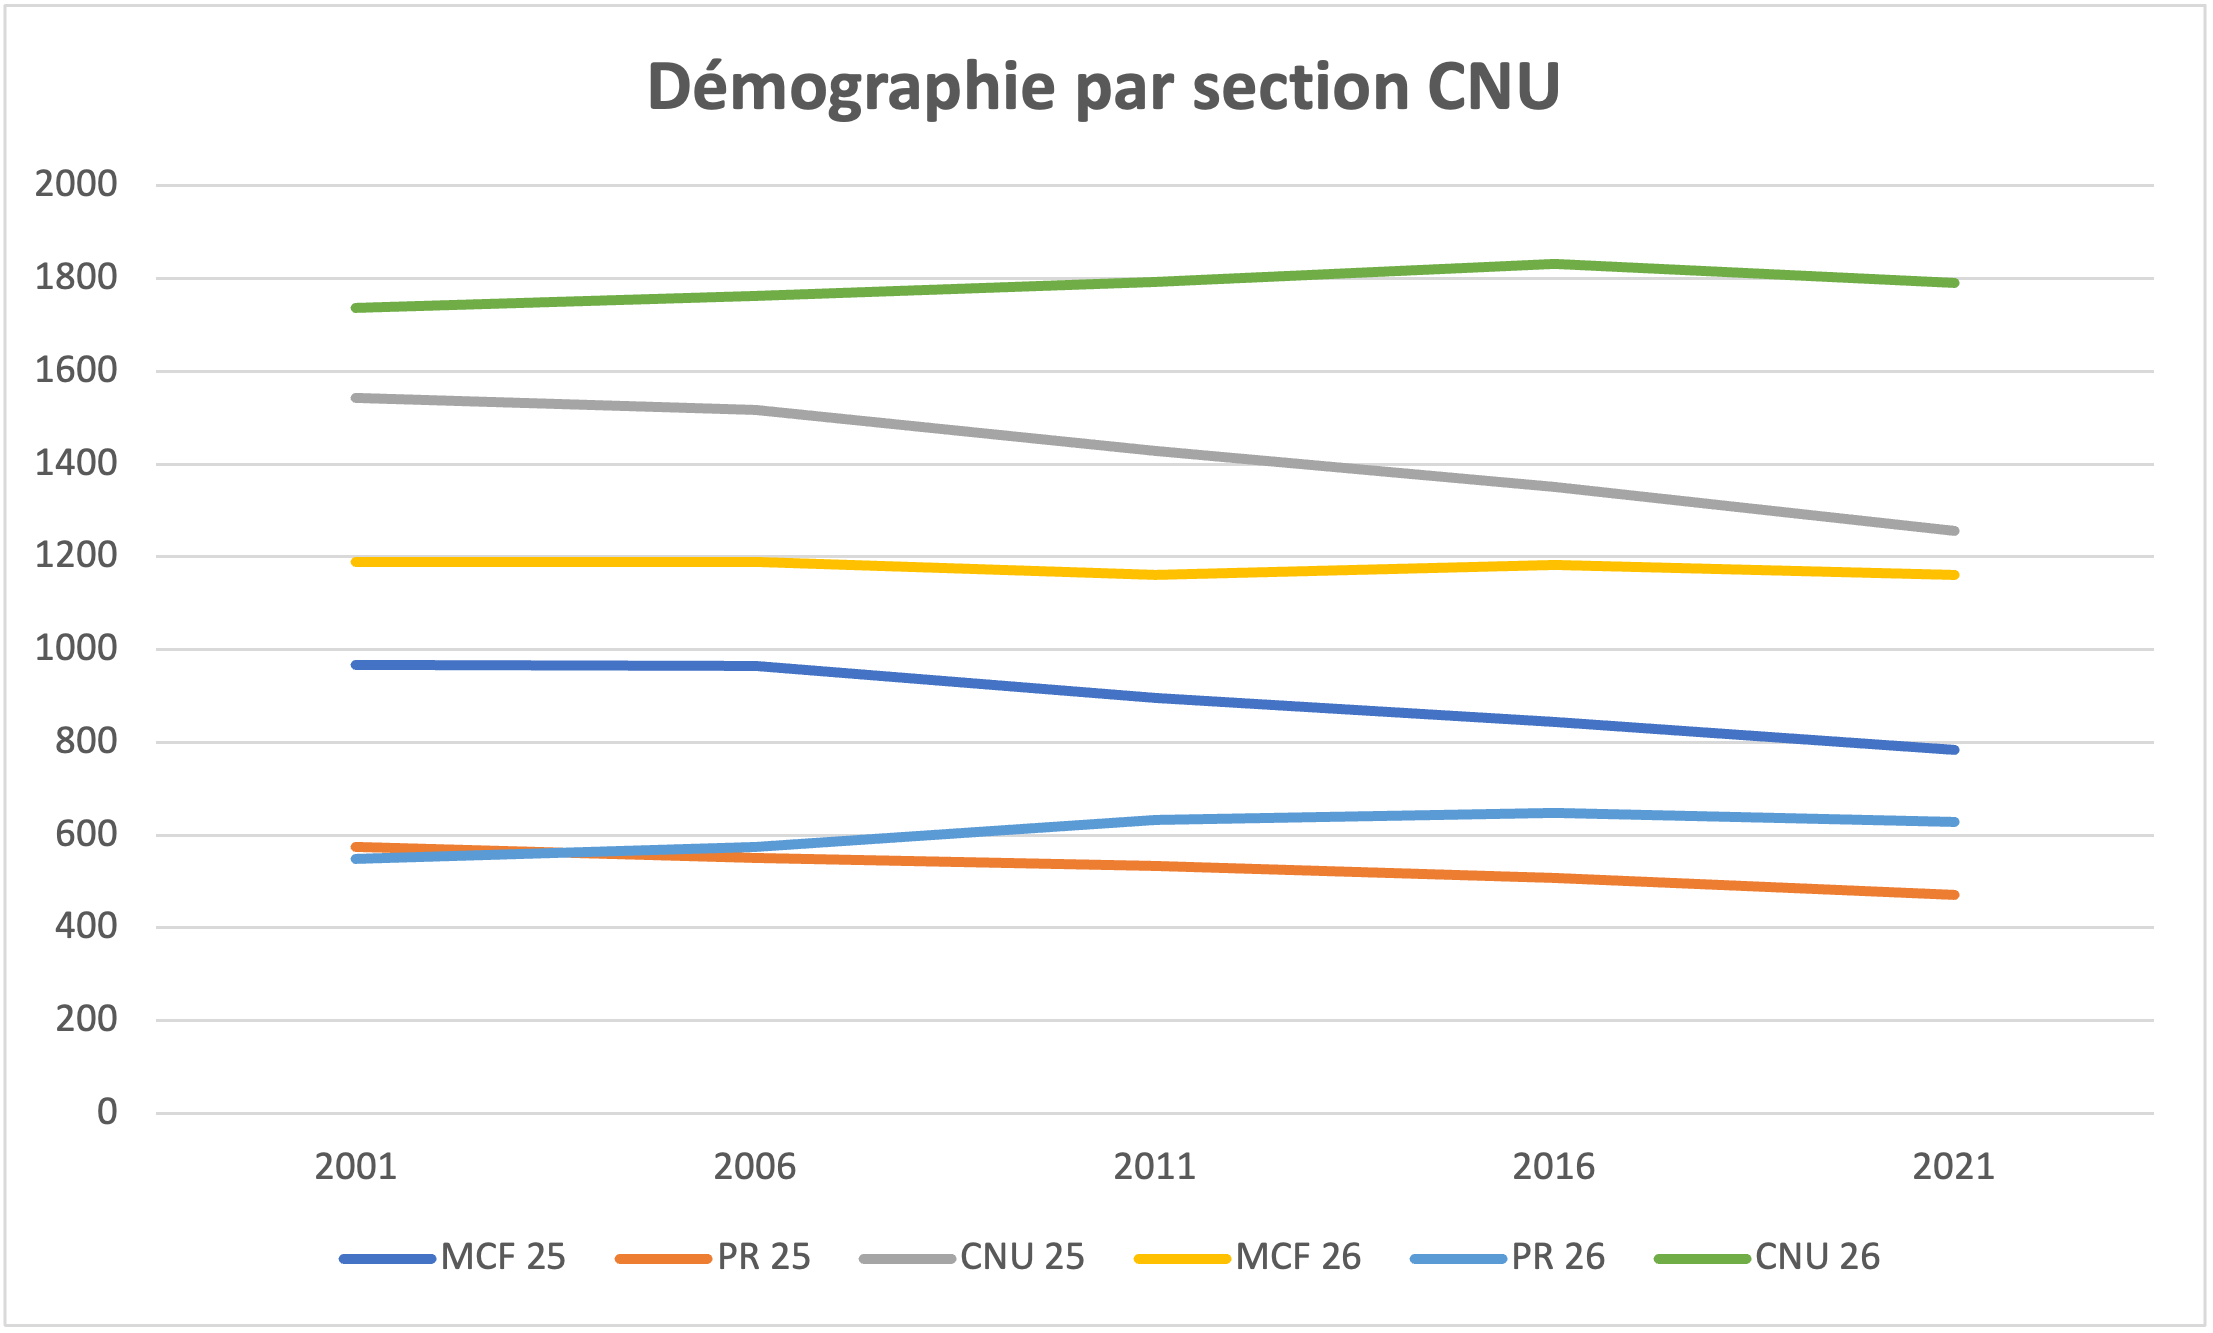
\includegraphics[width=8.5cm]{Images/cnu_demographie_2021}
}
\hfill
\subfloat[\'Evolution du nombre de postes publi\'es au concours pour les sections 25 et 26 du CNU (sessions synchronis\'ees)]{
\label{fig.cnu.postes}%
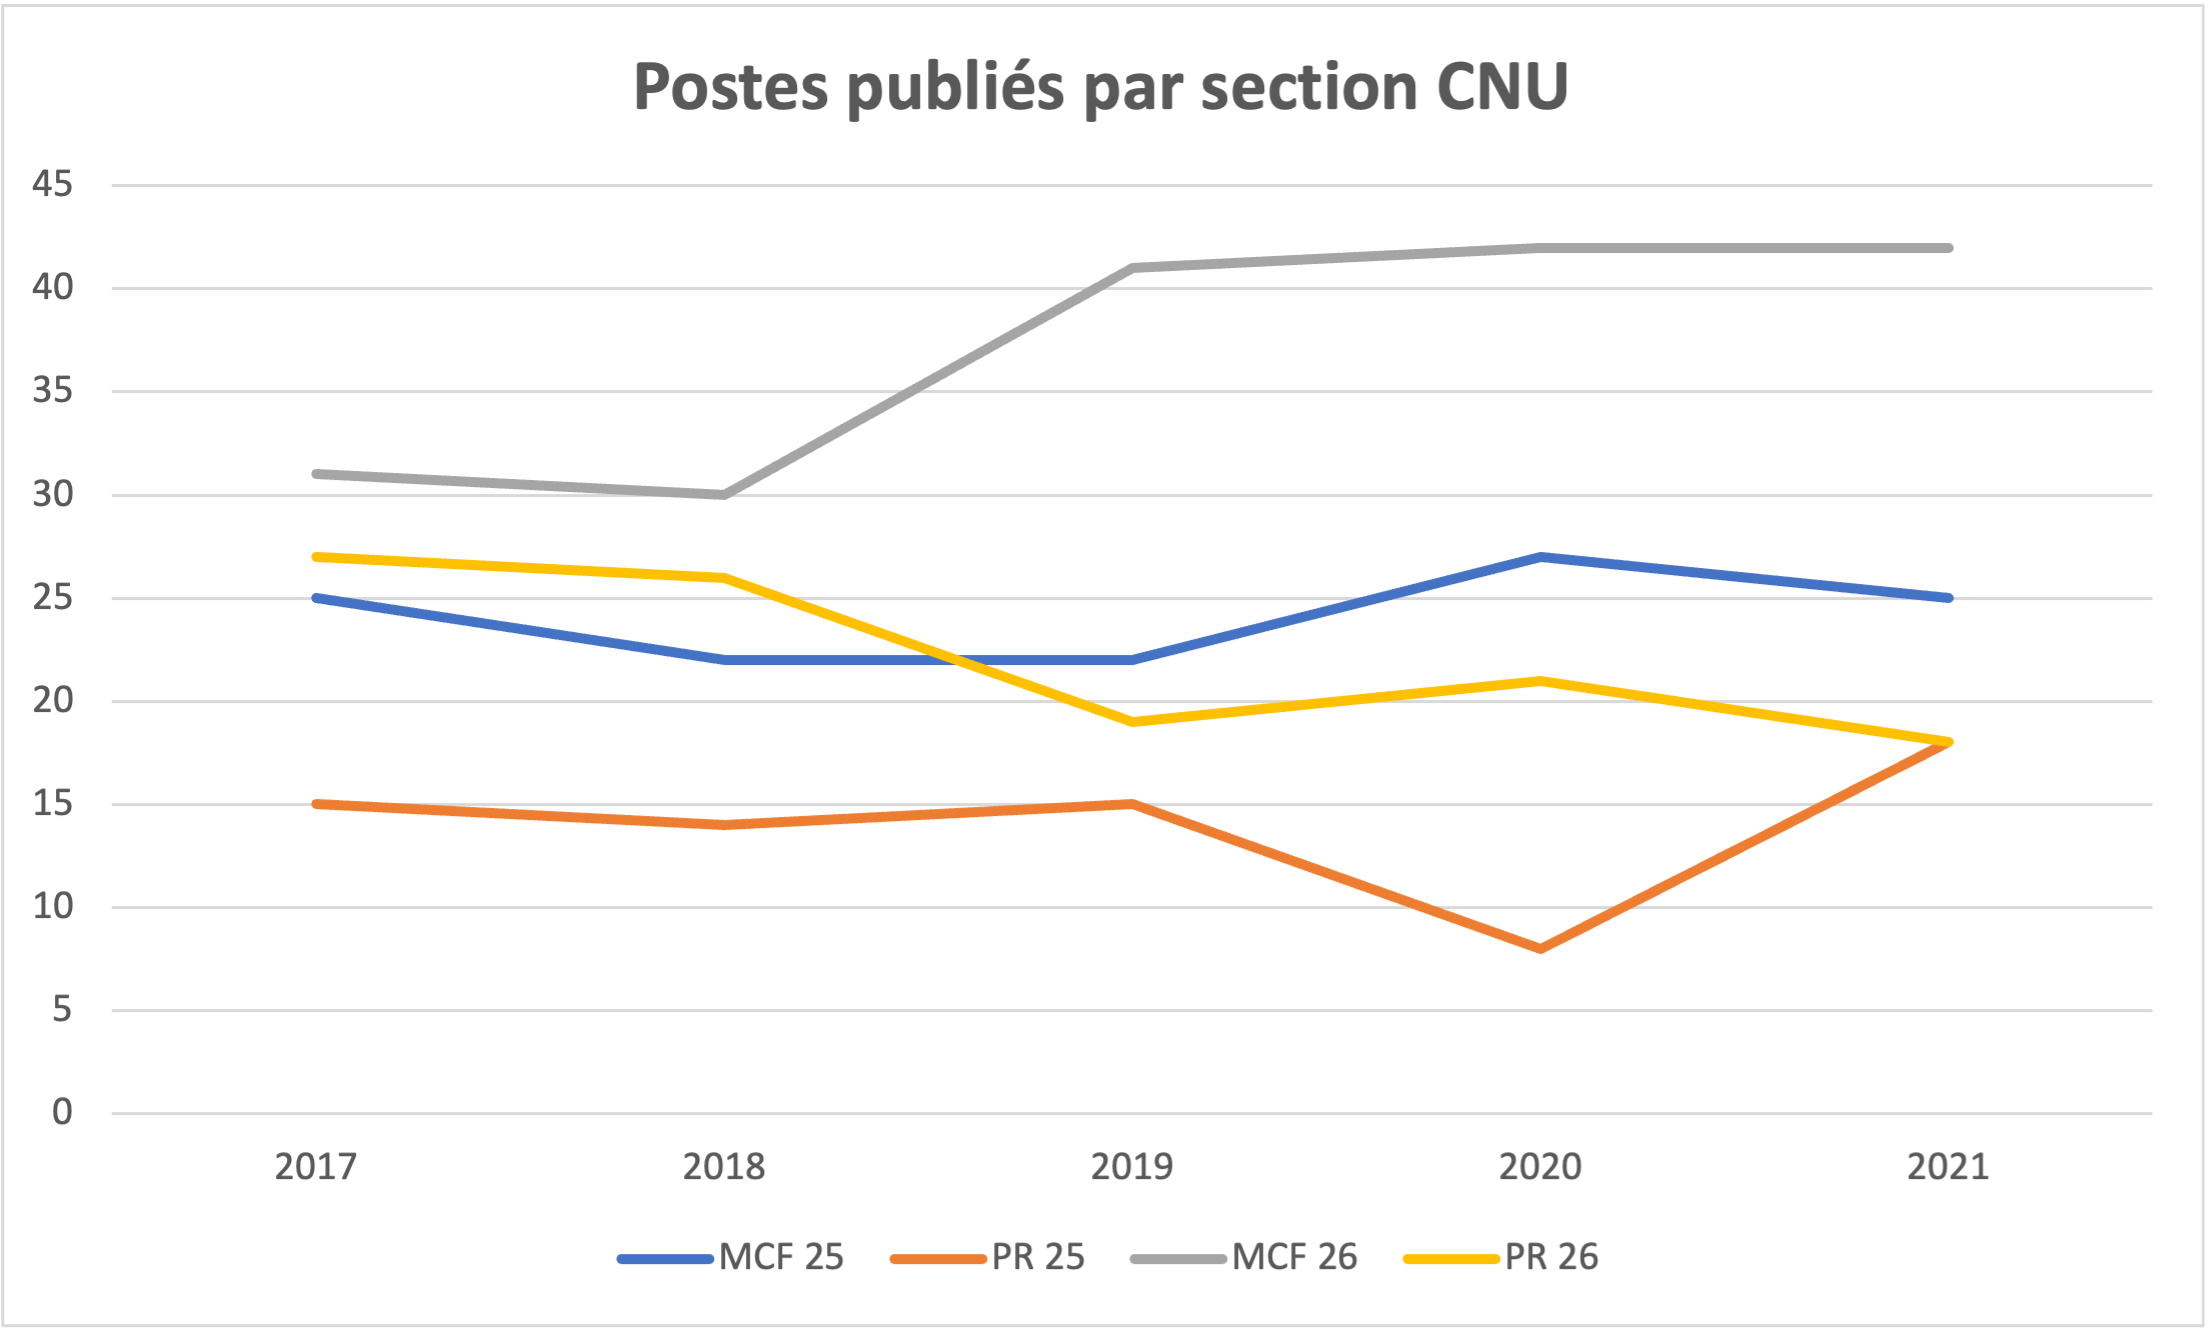
\includegraphics[width=8.5cm]{Images/cnu_nb_postes_2021}
}
\hfill
\begin{center}
\subfloat[\'Evolution du taux de pression (\textit{i.e.}, nombre de candidat\mp e\mp s/nombre de postes) pour les sections 25 et 26 du CNU (sessions synchronis\'ees)]{\label{fig.cnu.pression}%
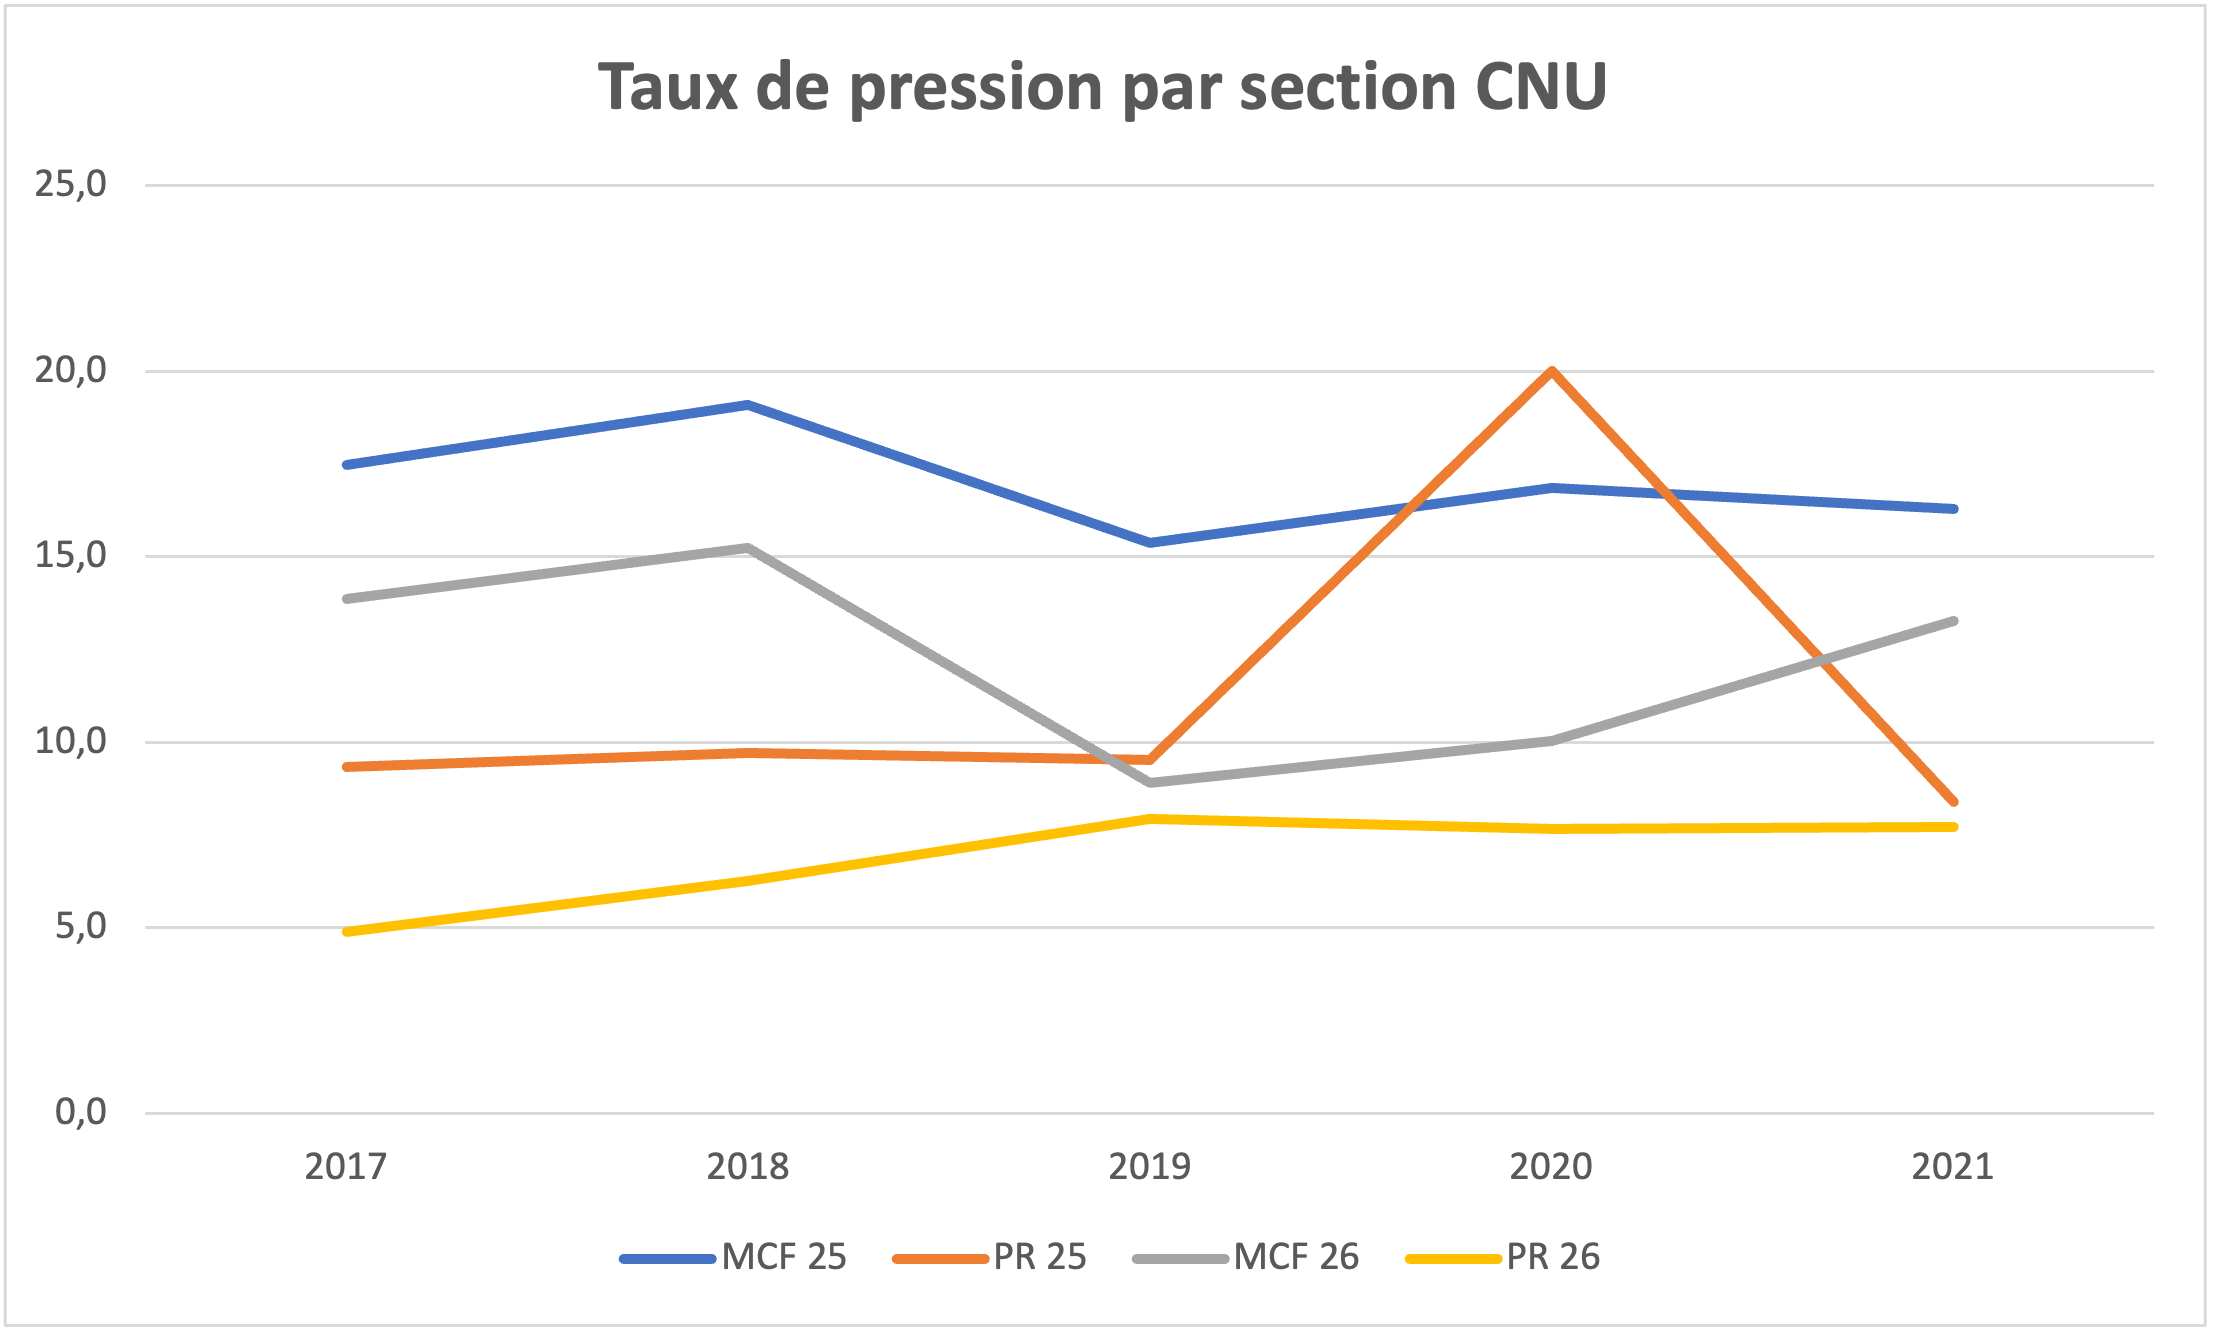
\includegraphics[width=8.5cm]{Images/cnu_taux_pression_2021}
}
\end{center}
\caption{Statistiques des postes d'enseignant\mp e\mp s-chercheur\mp euses au minist\`ere (MESRI)}
\label{fig.cnu}
\end{figure}


%\begin{figure}[p]
%\subfloat[\'Evolution du nombre de qualifi\'e\mp e\mp s]{\label{fig.qualif}%
%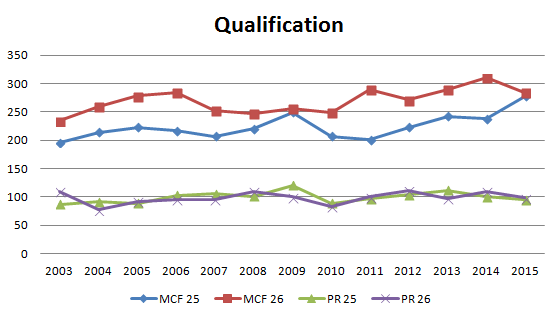
\includegraphics[width=8.5cm]{Images/qualif}
%}
%\hfill
%\subfloat[\'Evolution du nombre de postes]{\label{fig.postes}%
%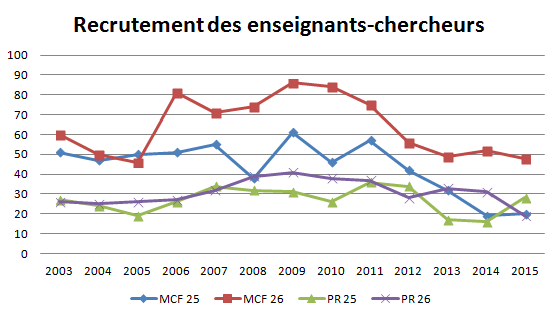
\includegraphics[width=8.5cm]{Images/recrut_EC}
%}
%\caption{Statistiques de recrutement en sections 25 et 26 du CNU (sessions synchronis\'ees)}\label{fig.recrut}
%\end{figure}

\paragraph*{Sources} Ces donn\'es ont \'et\'e compil\'ees \`a partir de rapports publics que nous vous invitons \`a consulter pour avoir davantage de d\'etails
\begin{itemize}
\item CNU : 
\url{https://www.enseignementsup-recherche.gouv.fr/fr/fiches-demographiques-des-sections-du-conseil-national-des-universites-cnu-83047}
\item Rapport sur la parit\'e dans la communaut\'e : \url{https://parite.math.cnrs.fr/effectifs.html}
\end{itemize}

% --- \`a mettre \`a jour
%Si l'on regarde plus en d\'etails les op\'erations de recrutement sur la d\'ecennie pass\'ee, on
%constate une d\'ecorr\'elation entre le nombre de qualifi\'e\mp e\mp s (constant voire en augmentation pour les MCF en section~26 
%-- voir Figure~\ref{fig.qualif})
%et le nombre de postes ouverts (voir Figure~\ref{fig.postes}). 
%Quant \`a l'\'ecart entre la date de qualification et la date de recrutement, il n'\'evolue pas de mani\`ere flagrante
%(voir Table~\ref{tab.recrut.anter}) : l'essentiel des recrutements s'effectue dans les 2 ans suivant la qualification.

%\begin{table}
%\begin{center}
%\begin{tabular}{*{7}{c}}
%\toprule
%&& $N-4$ & $N-3$ & $N-2$ & $N-1$ & $N$ \\
%\midrule
%2015 	& PR 25 & 1 & 3 & 5 & 6 & 7 \\
%	& PR 26 &  & 1 & 2 & 5 & 8 \\
%	& MCF 25 &  & 3 &  & 6 & 7 \\
%	& MCF 26 & 3 & 1 & 4 & 14 & 14 \\
%	\midrule
%2014 	& PR 25 &  &  & 2 & 2 & 7 \\
%	& PR 26 & 1 & 3 & 6 & 4 & 10 \\
%	& MCF 25 &  & 2 & 1 & 6 & 7 \\
%	& MCF 26 & 1 & 1 & 3 & 16 & 23 \\
%\midrule
%2013 	& PR 25 & 1 & 2 & 3 & 2 & 2 \\
%	& PR 26 & 1 & 1 & 1 & 5 & 15 \\
%	& MCF 25 &  & 3 & 1 & 9 & 17 \\
%	& MCF 26 &  &  & 5 & 13 & 25 \\
%\midrule
%2012	& PR 25 &  & 2 & 7 & 7 & 10 \\
%	& PR 26 & 2 & 2 & 2 & 5 & 10 \\
%	& MCF 25 & 1 & 5 & 1 & 12 & 21 \\
%	& MCF 26 & 1 & 1 & 6 & 13 & 32 \\
%\midrule
%2011 	& PR 25 & 1 & 3 & 2 & 5 & 15 \\
%	& PR 26 & 2 & 2 & 4 & 2 & 12 \\
%	& MCF 25 & 1 & 4 & 4 & 13 & 29 \\
%	& MCF 26 &  & 4 & 3 & 9 & 48 \\
%\midrule
%2010 	& PR 25 &  &  & 2 & 9 & 10 \\
%	& PR 26 &  & 1 & 3 & 7 & 14 \\
%	& MCF 25 &  & 3 & 6 & 9 & 22 \\
%	& MCF 26 &  & 6 & 9 & 13 & 43 \\
%\midrule
%2009	& PR 25 & 2 & 3 & 6 & 13 & 24 \\
%	& PR 26 & 3 & 2 & 4 & 17 & 26 \\
%	& MCF 25 &  & 3 & 12 & 18 & 21 \\
%	& MCF 26 &  & 3 & 8 & 12 & 44 \\
%\bottomrule
%\end{tabular}
%\caption{Temps \'ecoul\'e entre la qualification et le recrutement (ann\'ee $N$)}\label{tab.recrut.anter}
%\end{center}
%\end{table}
%
%


%%%%%%%%%%%%%%%%%%%%%%%%%%%%%%%%%%%%%%%%%%%%%
\section{Recrutement}
\label{recrutement}

Pour l'ensemble des disciplines, l'acc\`es aux corps
des ma\^itres de conf\'erences et des professeur\mp e\mp s des universit\'es comporte
g\'en\'eralement 2 \'etapes~:
\begin{enumerate}
\item la qualification aux fonctions
de ma\^\i tre de conf\'erences et/ou aux fonctions de professeur\mp e des
universit\'es;
\item les concours de recrutement ouverts dans chaque \'etablissement
d'enseignement sup\'erieur aux candidats et candidates pr\'ealablement
qualifi\'e\mp e\mp s.
\end{enumerate}

La qualification est une \'etape obligatoire pour \^etre \'eligible \`a une candidature \`a l'un de ces 2 corps. Pour les MCF titulaires et EC titulaires assimil\'e\mp e\mp s au corps des ma\^itres de conf\'erences relevant de la fonction publique française, la qualification est de droit apr\`es l'obtention de l'Habilitation \`a Diriger des Recherches (HDR). En cons\'equence, ils/elles ne doivent plus faire de demande de qualification aux fonctions de professeur\mp e des universit\'es. \`A l'exception de ce cas de figure, le processus de qualification est supervis\'e par le Conseil national des universit\'es (CNU : le fonctionnement de cet organisme est d\'ecrit en d\'etail dans le chapitre \ref{CNU}). 


La proc\'edure de recrutement proprement dite est quant \`a elle g\'er\'ee de mani\`ere autonome par les universit\'es elles-m\^emes. Pour chaque poste au concours, un jury, appel\'e comit\'e de s\'election, est constitu\'e ({\em cf.} Section \ref{sec. comiteselection}). Le comit\'e de s\'election examine les dossiers, \'etablit la liste des candidates et candidats qu'il souhaite entendre, et apr\`es avoir proc\'ed\'e aux auditions, il d\'elib\`ere sur les candidatures et \'emet un classement, \`a la majorit\'e des voix de ses membres. C'est au vu de l'avis \'emis par le comit\'e de s\'election que le Conseil d'administration propose le nom de la candidate ou du candidat s\'electionn\'e\mp e ou, le cas \'ech\'eant, une liste de candidat\mp e\mp s class\'e\mp e\mp s par ordre de pr\'ef\'erence.

Des informations sur les phases de qualification et de concours de recrutement peuvent \^etre trouv\'ee sur le site du minist\`ere (Galaxie) : \url{https://www.galaxie.enseignementsup-recherche.gouv.fr/ensup/candidats.html} ou sur le site de l'Op\'eration Postes \url{http://postes.smai.emath.fr}.



\subsection{Comit\'e de s\'election}\label{sec. comiteselection}
\index{Comit\'e de s\'election}

Les textes relatifs au comit\'e de s\'election peuvent \^etre trouv\'es au lien suivant :
\href{http://www.legifrance.gouv.fr/affichTexte.do;jsessionid=E1D1583A8C612508D9955CAB27DB96E0.tpdjo12v_3&dateTexte%
=?cidTexte=JORFTEXT000000520453&categorieLien=cid}{D\'ecret 84-431 du 6 juin 1984, version consolid\'ee du 01 janvier 2015}. 
On pourra aussi consulter le Code de l'Education, article L952-6-1 sur le
site \url{https://www.legifrance.gouv.fr/}.


Un comit\'e de s\'election est constitu\'e pour chaque emploi \`a pourvoir. Il constitue le jury du concours 
(D\'ecision du Conseil d'Etat 316927 du 15 d\'ecembre 2010 ; 317314 et 329584 du 9 f\'evrier 2011). 
Le Conseil d'administration, si\'egeant en formation
restreinte aux repr\'esentants \'elus des enseignant\mp e\mp s-chercheur\mp euse\mp s, des chercheur\mp euse\mp s et personnels assimil\'es, d\'elib\`ere
une premi\`ere fois pour pr\'eciser l'effectif total du comit\'e, entre 8 et 16 personnes, le nombre des membres choisis hors de
l'\'etablissement et le nombre de ceux choisis parmi les enseignants et enseignantes de la discipline concern\'ee. Au cours d'une
seconde d\'elib\'eration, il adopte la liste des membres, lesquels sont propos\'es par le\mp la pr\'esident\mp e ou le\mp la directeur\mp ice de
l'\'etablissement qui a recueilli l'avis de la Commission de la recherche.

Le comit\'e de s\'election est compos\'e de membres ext\'erieurs et de membres \og locaux\fg{}. Il si\`ege valablement si la moiti\'e de ses membres sont pr\'esents \`a la s\'eance, parmi lesquels une moiti\'e au moins de membres ext\'erieurs \`a l'\'etablissement. Sont consid\'er\'es comme membres ext\'erieurs \`a l'\'etablissement les enseignant\mp e\mp s-chercheur\mp euse\mp s et personnels assimil\'es qui ne sont pas \'electeur\mp ice\mp s pour les \'elections
au Conseil d'administration ; peuvent \^etre choisis des universitaires et des chercheuses et chercheurs d'institutions \'etrang\`eres,
d'un rang au moins \'egal \`a celui auquel postulent les candidat\mp e\mp s. La composition de chaque comit\'e est rendue
publique avant le d\'ebut de ses travaux.

Lorsqu'il s'agit d'un recrutement de ma\^itre de conf\'erences, le comit\'e de s\'election est compos\'e \`a parit\'e de MCF
et personnels assimil\'es et de PR et personnels assimil\'es. Pour un recrutement de professeur\mp e, seuls des PR et
personnels assimil\'es doivent former le comit\'e. Le Conseil d'administration choisit le ou la pr\'esident\mp e du comit\'e parmi les
membres du comit\'e.

Le comit\'e doit comprendre autant de femmes que d’hommes, avec des dispositions transitoires pour les comit\'es PR de certaines sections du CNU 
(comme la 25\`eme section) o\`u le pourcentage de femmes est faible.

Il faut signaler que nul ne peut appartenir simultan\'ement \`a des comit\'es de s\'election en activit\'e dans plus de 3
\'etablissements. Un comit\'e cesse son activit\'e \`a la date \`a laquelle il transmet ses avis au Conseil d'administration
de l'\'etablissement.

Un comit\'e de s\'election peut \^etre commun \`a plusieurs \'etablissements associ\'es \`a cette fin, notamment dans le
cadre d'un p\^ole de recherche et d'enseignement sup\'erieur ({\em cf.}, Section \ref{Regroupements}).

Le comit\'e de s\'election examine les dossiers des candidat\mp e\mp s \`a un recrutement, par la voie de la mutation, du
d\'etachement ou du concours. Notons que les articles 35 et 51 du statut \'etablissant la priorit\'e des mutations sur les concours ont \'et\'e abrog\'es : les mutations sont trait\'ees en m\^eme temps que les candidat\mp e\mp s demandant un premier recrutement en tant que MCF ou PR.
Le comit\'e de s\'election peut toutefois soumettre au Conseil d'administration des avis distincts pour chacune des 3 voies de recrutement.

Lors d'une seconde r\'eunion, le comit\'e de s\'election auditionne les candidat\mp e\mp s retenu\mp e\mp s, d\'elib\`ere sur les candidatures, \'emet un avis motiv\'e sur chaque candidature et, le cas \'ech\'eant, sur le classement retenu. Le comit\'e de s\'election se prononce \`a la majorit\'e des voix des membres pr\'esents. En cas de partage des voix, le pr\'esident du comit\'e a voix pr\'epond\'erante. Ces avis sont transmis au Conseil
d'administration, apr\`es quoi il est mis fin \`a l'activit\'e du comit\'e. Les avis sont communiqu\'es aux candidat\mp e\mp s sur leur demande. 

Le CA de l'\'etablissement si\`ege en formation
restreinte aux enseignant\mp e\mp s-chercheur\mp euse\mp s et personnels assimil\'es d'un rang au moins \'egal \`a celui de l'emploi
postul\'e. Il d\'elib\`ere \`a partir des avis formul\'es par le comit\'e de s\'election et peut, s'il l'estime n\'ecessaire, se faire communiquer toute pi\`ece du dossier des candidat\mp e\mp s. Il propose au ministre charg\'e de l'enseignement sup\'erieur le nom de la candidate ou du candidat s\'electionn\'e\mp e ou une liste de candidat\mp e\mp s class\'e\mp e\mp s par ordre de pr\'ef\'erence. La nomination dans le corps des MCF rel\`eve toujours de la comp\'etence du ministre, celle dans le corps des PR de la comp\'etence du ou de la Pr\'esident\mp e de la R\'epublique.

Le\mp La pr\'esident\mp e ou le\mp la directeur\mp ice de l'\'etablissement peut \'emettre un avis d\'efavorable motiv\'e sur le candidat retenu par
le CA ou sur l'un ou l'une des candidat\mp e\mp s class\'e\mp e\mp s ; en aucun cas, il\mp elle ne peut modifier l'ordre de la liste de classement.
Lorsque l'emploi \`a pourvoir est affect\'e \`a une \'ecole ou \`a un institut faisant partie d'une universit\'e, le\mp la pr\'esident\mp e ou
le\mp la directeur\mp ice de l'\'etablissement ne peut transmettre le nom du candidat ou de la candidate s\'electionn\'e\mp e ou la liste de classement si,
dans les 15 jours suivant la r\'eunion du Conseil d'administration, le\mp la directeur\mp ice de l'\'ecole ou de l'institut a \'emis un
avis d\'efavorable motiv\'e sur ce recrutement.

Concernant les mutations, sont admis \`a faire acte de candidature \`a la mutation sur un poste donn\'e les MCF qui, \`a la date de cl\^oture des inscriptions de ce poste (indiqu\'ee sur le site du minist\`ere), ont exerc\'e des fonctions d'enseignant\mp e-chercheur\mp euse en position d'activit\'e pendant au moins 3 ans dans l'\'etablissement o\`u ils\mp elles sont affect\'e\mp e\mp s, le stage \'etant pris en compte dans la d\'etermination de cette m\^eme p\'eriode. S'ils\mp elles ne justifient pas, \`a cette date, de 3 ans de fonctions d'enseignant\mp e-chercheur\mp euse en position d'activit\'e dans l'\'etablissement o\`u ils\mp elles sont affect\'e\mp e\mp s, les candidat\mp e\mp s ne peuvent d\'eposer une demande de mutation qu'avec l'accord de leur chef d'\'etablissement d'affectation, donn\'e apr\`es avis favorable du Conseil d'administration en formation restreinte aux enseignant\mp e\mp s-chercheur\mp euse\mp s et assimil\'es de rang au moins \'egal, ainsi que, le cas \'ech\'eant, de la ou du directeur\mp ice de l'institut ou de l'\'ecole faisant partie de l'universit\'e.

Les membres d'un comit\'e de s\'election peuvent participer aux r\'eunions en utilisant tout moyen de 
t\'el\'ecom\-munication permettant leur identification et leur participation effective : ils et elles sont alors r\'eput\'e\mp e\mp s pr\'esent\mp e\mp s pour
tous les calculs de quorum et de majorit\'e ; toutefois le comit\'e ne peut si\'eger valablement si le nombre des
membres physiquement pr\'esents est inf\'erieur \`a quatre.
Les candidates et candidats s\'electionn\'e\mp e\mp s pour l'audition peuvent demander \`a \^etre entendu\mp e\mp s par les m\^emes moyens de
t\'el\'ecommunication.

Pour de plus amples informations, vous pouvez consulter la FAQ sur le site Galaxie : \url{https://www.galaxie.enseignementsup-recherche.gouv.fr/ensup/etab_FAQ_comites_selection.html}.

\subsection{Ma\^\i tres de conf\'erences}

Les ma\^itres de conf\'erences sont recrut\'e\mp e\mp s par concours ouverts par \'etablissement.

\subsubsection*{1\iere{} \'etape : inscription sur la liste nationale de qualification}

Cette inscripion est obligatoire pour pouvoir participer \`a la
deux\`eme \'etape du concours. Tout titulaire d'un doctorat ou d'un
dipl\^ome \'equivalent peut poser sa candidature. D'autres voies
d'acc\`es, moins courantes, sont n\'eanmoins possibles : justifier de
3 ann\'ees d'activit\'e professionnelle effective au cours des six
ann\'ees pr\'ec\'edentes \`a l'exclusion des activit\'es
d'enseignant\mp e ou de chercheur\mp euse, \^etre enseignant\mp e associ\'e\mp e \`a temps
plein, \^etre d\'etach\'e\mp e dans le corps des ma\^itres de
conf\'erences ou bien appartenir au corps de charg\'e\mp e de recherche
ou \`a un corps de chercheur\mp euse. Les conditions et la forme de la
demande d'inscription sur la liste de qualification sont
pr\'ecis\'ees dans un arr\^et\'e publi\'e chaque ann\'ee au Journal
officiel.

Habituellement, les candidatures se d\'eclarent entre mi-septembre et mi-octobre, 
par inscription sur le site Antares de Galaxie : \url{https://galaxie.enseignementsup-recherche.gouv.fr/antares/can/index.jsp}.
Le nom des rapporteur\mp ice\mp s est mis en ligne \`a partir de la fin novembre et 
les candidats et candidates ont jusqu'\`a fin d\'ecembre pour envoyer leurs dossier apr\`es avoir au pr\'ealable soutenu
leur th\`ese (mi-d\'ecembre).
Le CNU se r\'eunit en d\'ebut d'ann\'ee et les listes des candidates et candidats qualifi\'e\mp e\mp s sont publi\'ees vers f\'evrier.

Le dossier de candidature comprend notamment une
description des activit\'es dans l'enseignement, la recherche ou
l'administration, et pr\'esente 3 exemplaires des travaux de la candidate ou du candidat,
ouvrages ou articles. Il est examin\'e par la section du CNU
comp\'etente pour la discipline. Pour la pr\'eparation du dossier, on peut se r\'ef\'erer au texte officiel sur le site de Galaxie
ou au site de l'Operation Postes : \url{http://postes.smai.emath.fr/2015/CONCOURS/qualification/index.php}.

Pour tout renseignement sur la constitution du dossier et le calendrier exact de la proc\'edure de qualification, 
vous pouvez vous r\'ef\'erer \`a la page officielle sur Galaxie : \url{https://www.galaxie.enseignementsup-recherche.gouv.fr/ensup/cand_qualification_droit_commun.htm}.

Le pourcentage de dossiers valid\'es
varie fortement suivant les disciplines. En math\'ematiques
(sections 25 et 26), il oscille autour de 75\,\% selon les bilans r\'edig\'es par les CNU 
\href{http://cnu25.emath.fr/}{25} et \href{http://cnu26.emath.fr/}{26} chaque ann\'ee. Notons que peut
\'eventuellement \^etre effectu\'ee
une demande d'inscription aupr\`es de plusieurs sections du CNU.

\subsubsection*{2\ieme{} \'etape~: les concours par \'etablissement}

Les concours sont ouverts dans les universit\'es, instituts ou
\'ecoles, en fonction du ou des postes \`a pourvoir. La plupart des
recrut\'e\mp e\mp s le sont sur le concours ouvert aux titulaires d'un
doctorat ou d'un dipl\^ome \'equivalent. Trois autres concours
existent n\'eanmoins. Le premier est r\'eserv\'e aux enseignantes et enseignants
titulaires du second degr\'e en fonction dans l'enseignement
sup\'erieur depuis 3 ans et titulaires d'un doctorat, et aux
pensionnaires ou anciens pensionnaires d'\'ecoles fran\c{c}aises \`a
l'\'etranger. Le deux\`eme est r\'eserv\'e aux candidats et candidates comptant
quatre ann\'ees d'activit\'e professionnelle effective au cours des
sept ann\'ees pr\'ec\'edentes, \`a l'exclusion des activit\'es
d'enseignant\mp e ou de chercheur\mp euse, et aux enseignant\mp e\mp s associ\'e\mp e\mp s \`a
temps plein.
Le dernier est r\'eserv\'e aux enseignant\mp e\mp s titulaires de l'Ecole nationale sup\'erieure d'arts et m\'etiers (ENSAM).

Les concours sont ouverts par arr\^et\'e du ministre charg\'e de
l'enseignement sup\'erieur. Les conditions et les modalit\'es du
d\'ep\^ot des candidatures sont pr\'ecis\'ees dans les arr\^et\'es
publi\'es au Journal officiel. Les candidatures sont
appr\'eci\'ees par les instances comp\'etentes des
\'etablissements~:
les comit\'es de s\'election et le Conseil d'administration.

L'\^age moyen du recrutement sur un poste de ma\^\i  tre de
conf\'erences \'etait en 2021 de 33 ans toutes sections sciences confondues. Pour obtenir d'autres statistiques, vous pouvez consulter les bilans des campagnes de recrutement mis en ligne r\'e\-gu\-li\`erement :
{\url{https://www.enseignementsup-recherche.gouv.fr/cid22708/bilans-statistiques.html}}

\subsection{Professeur\mp e\mp s des universit\'es}

Sous r\'eserve des dispositions particuli\`eres concernant les disciplines juridiques, politiques,
\'economiques et de gestion, les professeur\mp e\mp s des universit\'es sont recrut\'e\mp e\mp s par concours ouverts par \'etablissement.

\subsubsection*{1\iere{} \'etape : inscription sur la liste nationale de qualification}

Cette inscripion est obligatoire pour pouvoir participer \`a la deux\`eme \'etape du concours. N\'eanmoins, les MCF titulaires et EC titulaires assimil\'e\mp e\mp s au corps des ma\^itres de conf\'erences relevant de la fonction publique française n'ont d\'esormais plus de d\'emarches particuli\`eres \`a faire car ils sont r\'eput\'es qualifi\'es apr\`es l'obtention de l'Habilitation \`a Diriger des Recherches (HDR). Ne doivent donc faire la demande de qualification aux fonctions de professeur\mp e des universit\'es que les personnes titulaires de l'habilitation \`a diriger des recherches (HDR) ou d'un dipl\^ome \'equivalent n'ayant pas ce statut.

D'autres voies d'acc\`es, moins courantes, sont \'egalement possibles :
justifier de cinq ann\'ees d'activit\'e professionnelle effective au cours des huit ann\'ees pr\'ec\'edentes,
\`a l'exclusion des activit\'es d'enseignant\mp e ou de chercheur\mp euse,
\^etre enseignant\mp e associ\'e\mp e \`a temps plein,
\^etre d\'etach\'e\mp e dans le corps des professeur\mp e\mp s des universit\'es
ou bien appartenir au corps de directeur\mp ice\mp s de recherche ou \`a un corps de chercheur\mp euse.

Les statistiques de qualification sont de plus de 80\,\% dans les CNU 25 et 26.

\subsubsection*{2\ieme{} \'etape : les concours par \'etablissement}

Les concours sont ouverts dans les universit\'es, instituts ou \'ecoles, en fonction du ou des postes \`a pourvoir.
La plupart des recrut\'e\mp e\mp s le sont sur le concours ouvert aux titulaires d'une HDR ou d'un dipl\^ome \'equivalent.
Trois autres concours existent n\'eanmoins.

Le premier est r\'eserv\'e
aux MCF titulaires d'une HDR qui ont accompli cinq ann\'ees de service dans l'enseignement sup\'erieur ou qui ont \'et\'e charg\'e\mp e\mp s, 
depuis au moins 4 ans, d'une mission de coop\'eration culturelle,
scientifique et technique.

Le deux\`eme est r\'eserv\'e aux MCF titulaires de l'HDR qui ont accompli dix ann\'ees de service
(dont cinq en qualit\'e de MCF titulaire ou stagiaire) dans un \'etablissement d'enseignement sup\'erieur
de la Communaut\'e europ\'eenne, d'un \'etat faisant partie de l'accord sur l'espace \'economique
europ\'een,
ou dans un autre \'etablissement d'enseignement sup\'erieur au titre d'une mission de coop\'eration culturelle scientifique et technique, 
ou dans un \'etablissement public \`a caract\`ere scientifique et technologique.
Notons que la proc\'edure d'inscription sur la liste de qualification n'existe pas pour ce concours.
Le CNU formule, a posteriori, un avis sur les candidats retenus par l'\'etablissement.

Le dernier concours est ouvert
aux candidat\mp e\mp s ayant six ann\'ees d'activit\'e professionnelle effectives
durant les neuf ann\'ees pr\'ec\'edentes,
\`a l'exclusion des activit\'es d'enseignant\mp e ou de chercheur\mp euse,
aux enseignant\mp e\mp s associ\'e\mp e\mp s \`a temps plein,
aux MCF membres de l'Institut universitaire de France
et \`a des directeur\mp ice\mp s de recherche qui ont effectu\'e une d\'emarche de mobilit\'e
vers l'enseignement sup\'erieur, pour des nominations comme professeur\mp e des universit\'es de premi\`ere classe.

L'\^age moyen du recrutement sur un poste de  professeur\mp e des
universit\'es \'etait en 2021 de 45 ans toutes sections sciences confondues. Pour obtenir d'autres statistiques, vous pouvez consulter les bilans des campagnes de recrutement mis en ligne r\'e\-gu\-li\`erement :
{\url{https://www.enseignementsup-recherche.gouv.fr/cid22708/bilans-statistiques.html}}

%%%%%%%%%%%%%%%%%%%%%%%%%%%%%%%%%%%%%%%%%%%%%%%
\section{L'affectation}

Tout\mp e enseignant\mp e-chercheur\mp euse est rattach\'e\mp e \`a une unit\'e de formation
et de recherche (UFR), un d\'epar\-te\-ment, ou \`a un organe
\'equivalent, suivant l'\'etablissement d'affectation.

En ce qui concerne la recherche, il existe plusieurs types de
laboratoires de recherche dont les principaux, en ce qui concerne
les math\'ematiques, sont~:
\begin{itemize}
	\item les unit\'es mixtes de recherche (UMR)~: ces laboratoires,
		localis\'es dans les universit\'es, sont rattach\'es au CNRS~;
	\item les \'equipes d'accueil (EA)~: ces laboratoires sont
		reconnus et habilit\'es par le minist\`ere seul.
\end{itemize}

Dans certains \'etablissements, tels que 
les \'ecoles sup\'erieures du professorat et de l'\'education (ESPE), ancien IUFM,
ou encore dans
certaines \'ecoles d'ing\'enieurs ou IUT, il n'y a pas assez
d'enseignant\mp e\mp s-chercheur\mp euse\mp s par discipline pour monter une \'equipe de
recherche.
\index{Ecoles sup\'erieures du professorat et de l'\'education (ESPE)}
Quel que soit l'endroit de votre affectation, n'h\'esitez pas
\`a contacter le responsable du laboratoire de math\'e\-matiques le plus
proche pour demander votre rattachement. Cette demande sera, dans la
plupart des cas, re\c cue tr\`es positivement et vous permettra de ne
pas rester scientifiquement isol\'e\mp e. Tout\mp e enseignant\mp e-chercheur\mp euse
devrait \^etre rattach\'e\mp e \`a une \'equipe de
recherche ! Pour trouver les coordonn\'ees de ces structures, n'h\'esitez pas \`a
consulter l'annuaire de la communaut\'e math\'e\-matique
fran\c caise. \url{https://annuaire.emath.fr}

Nous rappelons de plus que tout\mp e nouvel\mp le enseignant\mp e-chercheur\mp euse (comme tout nouveau fonctionnaire)
a le droit de pr\'esenter une demande de reconstitution de carri\`ere : elle permet de faire reconna\^\i tre tout emploi comportant une activit\'e de recherche pr\'ec\'edant l'embauche \`a fin d'avancement d'\'echelon \`a l'anciennet\'e.

%%%%%%%%%%%%%%%%%%%%%%%%%%%%%%%%%%%%%%%%%%%%%%%
\section{L'\'evaluation}

Les EC sont \'evalu\'e\mp e\mp s lors de quelques moments importants de leurs carri\`eres.
Cette \'evaluation est (presque) exclusivement bas\'ee sur ses activit\'es de recherche
et d'encadrement doctoral (dans une moindre mesure).
Elle intervient lors~:
\begin{itemize}
\item de sa titularisation, au bout d'un an, sur d\'ecision de la Commission de la recherche de l'\'etablissement~;
\item des demandes de promotion, de primes (dispositif RIPEC),
de cong\'es pour recherche ou conversion
th\'ematique (CRCT), de d\'el\'egation et de d\'etachement (dans les
3 derniers cas, l'\'evaluation se fait surtout sur le projet de
recherche)~;
\item du passage de l'habilitation \`a diriger des recherches (HDR)~;
\item des concours de recrutement.
\end{itemize}
Un\mp e EC est \'egalement \'evalu\'e\mp e lors de l'\'evaluation de son laboratoire
et de son \'etablissement,
\'evaluations collectives par le Haut Conseil de l'Evaluation de la
Recherche et de l'Enseignement Sup\'erieur (HCERES, {\em cf.}, Chapitre \ref{HCERES}).
Les activit\'es de recherche de tous les membres du
laboratoire sont alors prises en compte, et la notion de \og publiant\fg{} est
alors utilis\'ee.
%
%Rappelons que le fonctionnement de l'HCERES est d\'etaill\'e dans le chapitre \ref{HCERES},
%et que de nombreuses informations sont disponibles sur son site
%\url{www.hceres.fr/}

D'autre part, le d\'ecret 2009-461 du 29 avril 2009 introduisait dans les missions du CNU l'\'evaluation individuelle des EC. 
Ce d\'ecret a \'et\'e fortement rejet\'e par tou\mp te\mp s les acteur\mp ice\mp s de la communaut\'e, en particulier les CNU 25 et 26.
Un moratoire avait alors \'et\'e annonc\'e pour la session 2012--2013. 
Ce d\'ecret a \'et\'e remplac\'e depuis par le d\'ecret 2014-997 du 2 septembre 2014 qui pr\'econise
d\'esormais un \og suivi de carri\`ere\fg{} quiquennal rempla\c{c}ant l'\'evaluation individuelle. Le suivi de carri\`ere est obligatoire mais certaines sections dont les sections 25 et 26 ont refus\'e de le faire. Parmi les m\'edias de contestation, citons par exemple : \url{http://www.sauvonsluniversite.com/spip.php?article3423}.

% \textit{Motions \'evaluation adopt\'ees le 2 f\'evrier 2010 par la section 25 (Math\'ematiques appliqu\'ees et applications des math\'ematiques) du CNU}
% 
% Motion 1 : Les membres de la section 25 du CNU r\'eunis le 2 f\'evrier 2010 rappellent que durant le mandat en cours ils refuseront de si\'eger pour une \'eventuelle session d'\'evaluation quadriennale.
% 
% \textit{Motions \'evaluation adopt\'ees le 3 f\'evrier 2010 par la section 26 (Math\'ematiques appliqu\'ees et applications des math\'ematiques) du CNU}
% 
% La section 26 du CNU a pris position le 4 f\'evrier 2010 contre la proposition de la CP-CNU de donner un avis sur tous les dossiers de demande de promotions, m\^eme pour les candidats \`a qui ne sera pas accord\'ee de promotion. La section consid\`ere en effet que c'est inutile, voire n\'efaste, car cela revient \`a mettre le doigt dans l'engrenage de l'\'evaluation quadriennale. Voici les motions vot\'ees :
% 
% Point 1 : \og Lors de la session d'attribution des promotions, la section CNU 26 n'\'emettra pas d'avis sur les dossiers des coll\`egues non promus." - Adopt\'e \`a l'unanimit\'e
% 
% Point 2 : \og Les membres de la section 26 r\'eunis le 3 f\'evrier 2010 rappellent leur refus de si\'eger pour une \'eventuelle session d'\'evaluation quadriennale durant leur mandat." - Unanimit\'e moins une abstention.


\index{Evaluation ! \`a l'universit\'e}
\index{Publiants}
\index{Haut Conseil de l'Evaluation de la
Recherche et de l'Enseignement Sup\'erieur (HCERES)}
\index{Cong\'e pour recherche ou conversion th\'e\-ma\-ti\-que (CRCT)}
\index{Habilitation \`a diriger des recherches (HDR)}

%%%%%%%%%%%%%%%%%%%%%%%%%%%%%%%%%%%%%%%%%
\section{L'enseignement}
\label{enseignement}

Outre leurs activit\'es de recherche, les EC assurent des enseignements. Le service statutaire est de 192 heures \og \'equivalent TD\fg{}. 
La conversion est : 1h cours (en pr\'esentiel)= 1,5 h \'eq. TD, les TP \'etant compt\'es comme les TD sauf s'il sont effectu\'es en heures compl\'ementaires. Donc un EC peut faire par exemple 192h de TD ou 60h de cours et 102h de TD 
(voir le d\'ecret \href{http://www.legifrance.gouv.fr/affichTexte.do?cidTexte=JORFTEXT000020552216&dateTexte=&categorieLien=id}{D\'ecret num\'ero 2009-460 du 23 avril 2009}).


\`A ce service commun, peuvent s'ajouter des heures
compl\'ementaires, parfois en nombre limit\'e dans certains \'etablissements (\href{http://www.legifrance.gouv.fr/affichTexte.do?cidTexte=JORFTEXT000000315917&dateTexte=20121122}{voir la modification de l'Arr\^et\'e du 6 novembre 1989 fixant les taux de r\'emun\'eration des heures compl\'ementaires}). Une heure est r\'emun\'er\'ee par une indemnit\'e non soumise \`a retenue pour pension et fix\'ee \`a 61,35 \euro~ pour les cours, 40,91 \euro~ pour les travaux pratiques et 27,26 \euro~ pour les travaux pratiques.

%\begin{table}[!ht]
%\begin{center}
%\begin{tabular}{|c|c|c|}
%\hline
%Cours & Travaux dirig\'es & Travaux pratiques\\
%\hline
%61,35 \euro & 40,91 \euro & 27,26 \euro\\
%\hline
%\end{tabular}
%\end{center}
%\end{table}

Les enseignant\mp e\mp s b\'en\'eficiant d'une d\'echarge statutaire de service de quelque
nature qu'elle soit, les enseignant\mp e\mp s en cong\'e pour recherche ou
conversion th\'ematique (CRCT), en cong\'e parental ou b\'en\'eficiant d'une
d\'echarge sollicit\'ee ne peuvent effectuer d'heures
compl\'ementaires. Notons enfin
que, ni les PRAG b\'en\'eficiant d'une d\'echarge pour
pr\'eparer leur th\`ese ou faire de la recherche,
ni les contrats doctoraux charg\'es d'enseignement,
ni les ATER ne peuvent effectuer d'heures compl\'ementaires.

La loi LRU sp\'ecifie express\'ement que le Conseil
d'administration pourra d\'efinir les principes g\'en\'eraux de
r\'epartition des obligations de service des personnels enseignants
entre leurs diff\'erentes activit\'es (enseignement, recherche,
administration, valorisation...), dans le respect des dispositions
statutaires et en fonction des besoins de l'\'etablissement.

\index{R\'ef\'erentiel des t\^aches}
\label{referentiel}
L'arr\^et\'e du 31 juillet 2009 institue \`a cet effet un r\'ef\'erentiel
national d'\'equivalence horaire, dont doit se saisir chaque \'etablissement
pour fixer son r\'ef\'erentiel propre. Ce travail est encore en cours dans bon nombre
d'\'etablissements, qui ont aussi le loisir, par l'interm\'ediaire de son pr\'esident,
de moduler le service d'un ou d'une enseignant\mp e-chercheur\mp euse \`a la hausse ou \`a la baisse (avec l'accord
explicite de l'int\'eress\'e). Pour plus de renseignements, on peut lire l'article 7 du d\'ecret 84-431 sur
\url{https://www.legifrance.gouv.fr/}.

\index{Travaux dirig\'es (TD)}\index{Travaux pratiques (TP)}
\index{R\'ef\'erentiel horaire}

%%%%%%%%%%%%%%%%%%%%%%%%%%%%%%%%%%%%%%%%%
\section{Carri\`ere et r\'emun\'eration}
\label{salairesEC}

Comme pour tout fonctionnaire, le traitement d'un\mp e EC est constitu\'ee
d'une r\'emun\'eration principale \`a laquelle s'ajoutent des indemnit\'es et des primes.

La r\'emun\'eration principale d'un\mp e EC augmente
p\'e\-rio\-di\-quement au fur et \`a mesure qu'il gravit les
\'echelons \`a l'int\'erieur de son grade. Cette progression se fait \`a l'anciennet\'e ({\em cf.}, Tables \ref{tab.avanc.MCF} et \ref{tab.avanc.PR}).
A chaque \'echelon correspond en effet un indice qui d\'etermine le montant de la
r\'emun\'eration principale. L'indice de r\'emun\'eration auquel le\mp la candidat\mp e est recrut\'e\mp e est d\'etermin\'e en fonction de ses dipl\^omes et de ses activit\'es professionnelles ant\'erieures. Le calcul est simple~: un point
d'indice a une certaine valeur fiduciaire (au 1er janvier 2023, la valeur est fix\'ee \`a 4,85 \euro) et le traitement est
calcul\'e par simple multiplication du nombre de points d'indice par
cette valeur nominale. La valeur du point d'indice est
r\'e\'evalu\'ee de mani\`ere \'episodique.
% \`A titre d'exemple, la valeur
% annuelle du point d'indice en date du 1er f\'evrier 2015 \'etait de
% 55,5635\,\euro{} brut. La pr\'ec\'edente r\'e\'evalutation, en
% date du 1er juillet 2010, correspond \`a une hausse de 0,5\,\% (ce qui,
% pour un MCF d\'ebutant, correspond \`a une augmentation de 10 euros
% brut mensuel). Notons que les r\'e\'evaluations successives depuis le 1er d\'ecembre
% 2002 correspondent \`a une augmentation totale de 5,85\, \%, et que l'inflation sur la m\^eme
% dur\'ee est d'environ 20,9\,\% d'apr\`es l'INSEE.

S'ajoutent ensuite \`a cette r\'emun\'eration principale diverses indemnit\'es
(r\'esidence, suppl\'ement familial)
et/ou diff\'erentes primes (RIPEC, primes administratives, ...)
ainsi que le paiement des \'eventuelles heures compl\'emen\-taires effectu\'ees
({\em cf.}, Section \ref{enseignement}).


\subsection{Grilles d'avancement et de salaires}\label{sec. grilles}

Le corps des MCF comporte 2 classes
(\textit{grades}):
\begin{itemize}
\item une classe normale, qui comprend 9 \'echelons~;
\item une hors-classe, qui comprend 6 \'echelons.
\end{itemize}

\begin{center}
\begin{table}[b!]
\begin{center}
\subfloat[MCF classe normale]{
\begin{tabular}{lcc}
\toprule
& Indice (INM)& Dur\'ee \\
\midrule
1\ier{} \'echelon &474&1 an \\
2\ieme{} \'echelon &531&2 ans et 10 mois\\
3\ieme{} \'echelon &584&2 ans et 10 mois\\
4\ieme{} \'echelon &643&2 ans et 10 mois\\
5\ieme{} \'echelon &693&2 ans et 10 mois\\
6\ieme{} \'echelon &739&3 ans et 6 mois\\
7\ieme{} \'echelon &769&2 ans et 10 mois\\
8\ieme{} \'echelon &803&2 ans et 10 mois\\
9\ieme{} \'echelon &830&\\
\bottomrule
\end{tabular}
}
\hfill
\subfloat[MCF hors-classe]{
\begin{tabular}{lcc}
\toprule
& Indice (INM)& Dur\'ee\\
\midrule
1\ier{} \'echelon &678&1 an\\
2\ieme{} \'echelon &716&1 an\\
3\ieme{} \'echelon &754&1 an\\
4\ieme{} \'echelon &796&1 an\\
5\ieme{} \'echelon &830&5 ans\\
6\ieme{} \'echelon & & \\
~\hspace{1cm}1\ier{} chevron &890&1 an\\
~\hspace{1cm}2\ieme{} chevron &925&1 an\\
~\hspace{1cm}3\ieme{} chevron &972& avancement \\
\'Echelon exceptionnel & & \\
~\hspace{1cm}1\ier{} chevron &972&1 an\\
~\hspace{1cm}2\ieme{} chevron &1013&1 an\\
~\hspace{1cm}3\ieme{} chevron &1067&  \\
\bottomrule
\end{tabular}
}
\caption{Grilles d'avancement des MCF}\label{tab.avanc.MCF}
\end{center}
\end{table}
\end{center}

\index{Ma\^\i tre de conf\'erences (MCF)!classe normale}
\index{Ma\^\i tre de conf\'erences (MCF)!hors-classe}

%\newpage
Le corps des PR comporte 3
classes (\textit{grades}):
\begin{itemize}
\item une seconde classe qui comprend 6 \'echelons~;
\item une premi\`ere classe qui comprend 3 \'echelons~;
\item une classe exceptionnelle qui comprend 2 \'echelons.
\end{itemize}

\begin{center}
\begin{table}[t!]
\begin{center}
\subfloat[PR seconde classe]{\small
\begin{tabular}{lcc}
\toprule
& Indice (INM)& Dur\'ee\\
\midrule
1\ier{} \'echelon &667&1 an\\
2\ieme{} \'echelon &705&1 an\\
3\ieme{} \'echelon &743&1 an\\
4\ieme{} \'echelon &785&1 an\\
5\ieme{} \'echelon &830&3 ans et 6 mois\\
6\ieme{} \'echelon & & \\
~\hspace{1cm}1\ier{} chevron &890&1 an\\
~\hspace{1cm}2\ieme{} chevron &925&1 an\\
~\hspace{1cm}3\ieme{} chevron &972& 3 ans et 6 mois\\
7\ieme{} \'echelon & &\\ 
~\hspace{1cm}1\ier{} chevron &972&1 an\\
~\hspace{1cm}2\ieme{} chevron &1013&1 an\\
~\hspace{1cm}3\ieme{} chevron &1067& \\
\bottomrule
\end{tabular}
}
\hfill
\subfloat[PR premi\`ere classe]{
\begin{tabular}{lcc}
\toprule
& Indice (INM)& dur\'ee\\
\midrule
1\ier{} \'echelon &830&3 ans\\
2\ieme{} \'echelon & &  \\
~\hspace{1cm}1\ier{} chevron &972&1 an\\
~\hspace{1cm}2\ieme{} chevron &1013&1 an\\
~\hspace{1cm}3\ieme{} chevron &1067&2 ans et 4 mois \\
3\ieme{} \'echelon & &  \\
~\hspace{1cm}1\ier{} chevron &1124&1 an\\
~\hspace{1cm}2\ieme{} chevron &1148&1 an\\
~\hspace{1cm}3\ieme{} chevron &1173& \\
\bottomrule
\end{tabular}
}

\subfloat[PR classe exceptionnelle]{
\begin{tabular}{lcc}
\toprule
& Indice (INM)& dur\'ee\\
\midrule
1\ier{} \'echelon & &  \\
~\hspace{1cm}1\ier{} chevron &1173&1 an\\
~\hspace{1cm}2\ieme{} chevron &1226&1 an\\
~\hspace{1cm}3\ieme{} chevron &1279& \\
2\ieme{} \'echelon & &  \\
~\hspace{1cm}1\ier{} chevron &1279&1 an\\
~\hspace{1cm}2\ieme{} chevron &1329&\\
\bottomrule
\end{tabular}
\normalsize}
\caption{Grilles d'avancement des PR}\label{tab.avanc.PR}
\end{center}
\end{table}
\end{center}


\index{Professeur\mp e des universit\'es (PR)!seconde classe}
\index{Professeur\mp e des universit\'es (PR)!premi\`ere classe}
\index{Professeur\mp e des universit\'es (PR)!classe exceptionnelle}


\`A l'exception des PR de classe exceptionnelle,
le passage d'un \'echelon au suivant (dans chaque classe) se fait
automatiquement, \`a l'{\em anciennet\'e}, selon le tempo indiqu\'e
dans les tableaux \ref{tab.avanc.MCF} et \ref{tab.avanc.PR}, o\`u l'on rapporte aussi les indices
nouveaux major\'es (INM). Pour le passage \`a la classe exceptionnelle, le nombre de promotions est calcul\'e chaque ann\'ee et d\'efini globalement, pour l'ensemble des sections, sous forme d'un pourcentage de promotions par rapport au nombre de \og promouvables\fg{} 
%({\em cf.}, par exemple le\href{www.legifrance.gouv.fr/affichTexte.do?cidTexte=JORFTEXT000025756970\&dateTexte=\&categorieLien=id}{lien sur Legifrance}.

Pour un\mp e MCF, le passage \`a la hors-classe se fait au {\em choix} (16 ans minimum
apr\`es le d\'ebut de carri\`ere~: il faut avoir atteint le
7\ieme{} \'echelon de la classe normale).
Pour un\mp e PR, le passage d'une classe \`a l'autre se fait \'egalement au {\em choix}.
Nous renvoyons \`a la section sur le Conseil national des universit\'es (CNU) pour la
description de l'attribution des promotions (\textit{c.f.}, Chapitre \ref{CNU}).

Des bonifications d'anciennet\'e peuvent \^etre accord\'ees aux EC
qui ont assur\'e un mandat de pr\'esident\mp e
ou de directeur\mp ice d'\'etablissement public d'enseignement sup\'erieur
ou qui s'engagent dans une d\'emarche de
mobilit\'e (par exemple une bonification d'anciennet\'e d'un an
pour un s\'ejour d'un an dans un organisme d'enseignement sup\'erieur
ou de recherche d'un autre \'etat de la Communaut\'e europ\'eenne,
{\em cf.}, le d\'ecret 2002-295 du 28 f\'evrier 2002).

\index{Conseil national des universit\'es (CNU)}
\index{Ma\^\i tre de conf\'erences (MCF)!promotions}
\index{Professeur des universit\'es (PR)!promotions}

On peut noter au passage que, d'apr\`es les donn\'ees de l'INSEE, le salaire initial d'un ou d'une ma\^\i tre de
conf\'erences (indice 454) a subi une diminution constante et r\'eguli\`ere
par rapport au SMIC de plus de 30\,\% depuis 1990 (passage de 2,07 au 01/01/1990 \`a 1,34 fois le SMIC au 01/01/2023)\ldots

%\subsection{Les indemnit\'es et les primes}

\subsection{Indemnit\'es et primes -- Le dispositif RIPEC}

La politique indemnitaire pour les EC est d\'efinie par la loi n° 2020-1674 du 24 d\'ecembre 2020 de programmation de la recherche pour les ann\'ees 2021 \`a 2030 (LPR). Les EC sont \'eligibles \`a des indemnit\'es statutaires et \`a des primes fix\'ees par le d\'ecret n° 2021-1895 du 29 d\'ecembre 2021 ayant conduit \`a la cr\'eation du r\'egime indemnitaire des personnels enseignants et chercheurs (RIPEC). Ce dispositif comprends 3 composantes. Toutes les informations sont disponibles sur : \url{https://www.enseignementsup-recherche.gouv.fr/fr/bo/22/Hebdo10/ESRH2204566X.htm}.

\subsubsection{La composante statutaire (C1)}
\label{ripec-C1}

Cette part indemnitaire est vers\'ee mensuellement \`a tous les EC qui accomplissent l'int\'egralit\'e de leur service. Elle remplace depuis 2022 la prime de recherche et d'enseignement sup\'erieur (PRES) qui \'etait attribu\'ee aux enseignants-chercheurs (d\'ecret n° 89-775 du 23 octobre 1989). D'ici \`a 2030, le montant annuel de l'indemnit\'e sera fix\'e chaque ann\'ee par arr\^et\'e. En 2022, il \'etait de 2800 \euro.

Les personnels plac\'es en d\'el\'egation, en cong\'e pour recherches ou conversions th\'ematiques ou en cong\'e pour projet p\'edagogique et aux personnels qui b\'en\'eficient de d\'echarges de service peuvent \'egalement b\'en\'eficier de cette ind\'emnit\'e. Ce n'est en revanche pas le cas des personnels qui perçoivent des r\'emun\'erations compl\'ementaires au titre de l'exercice d'une profession lib\'erale.

%Une prime annuelle de recherche est vers\'ee \`a toutes et tous les
%enseignant\mp e\mp s-chercheur\mp euse\mp s. Son montant est aujourd'hui de
%1244,98\,\euro{} brut. Elle est vers\'ee en 2 fois, aux mois de
%d\'ecembre et juillet. Elle est compatible avec le fait d'effectuer
%des heures compl\'ementaires, mais pas avec un cumul d'emploi.
%

\subsubsection{La composante fonctionnelle (C2)}

Cette indemnit\'e est li\'ee \`a l'exercices de fonctions ou responsabilit\'es particuli\`eres fix\'ees par le\mp la chef\mp fe de l'\'etablissement. Elle est vers\'ee mensuellement. Son montant annuel est plafonn\'e par arr\^et\'e minist\'eriel par groupes de fonctions ou de niveaux de responsabilit\'e. 

Tout comme la composante C1, il est n\'ecessaire de satisfaire ses obligations de service pour pouvoir en b\'en\'eficier. En revanche, \`a l'inverse de la composante C1, elle ne peut \^etre per\c{c}ues par les EC position de d\'el\'egation, en cong\'e pour recherches ou conversions th\'ematiques ou en cong\'e pour projet p\'edagogique, ou percevant des r\'emun\'erations compl\'ementaires au titre de l'exercice d'une profession lib\'erale.

\subsubsection{La prime individuelle (C3)}
\label{ripec-C3}

Cette prime remplace depuis 2022 la prime d'encadrement doctoral et de recherche (PEDR, d\'ecret n° 2009-851 du 8 juillet 2009). L'attribution de cette prime se fait suite un processus d'\'evaluation en plusieurs \'etapes.

Tout d'abord, les EC souhaitant b\'en\'eficier de cette prime doivent d\'eposer un dossier, comprenant notamment un rapport d'activit\'e de recherche et d'enseignement portant sur les 4 ann\'ees pr\'ec\'edant la candidature, sur l'application ELARA de Galaxie (\url{https://www.galaxie.enseignementsup-recherche.gouv.fr/ensup/cand_RIPEC.htm}). Le CNU rend ensuite un avis unique (tr\`es favorable, favorable ou r\'eserv\'e) et pr\'ecise au titre de quelle mission (recherche, p\'edagogie, vie collective) la prime est propos\'ee. Il peut s'agir d'une de ces missions, de plusieurs ou de l'ensemble d'entre elles.

Une fois les dossiers \'evalu\'es par le CNU, ils sont transmis au conseil acad\'emique si\'egeant en formation restreinte aux EC et personnels assimil\'es (CAFR), ou \`a l'organe comp\'etent, de l'\'etablissement de rattachement de l'EC. Ce dernier d\'esigne 2 rapporteurs par candidat\mp e de rang au moins \'egal \`a celui du ou de la candidat\mp e. Sur la bases de ces 2 rapports, le CA rend \`a son tour un avis unique (tr\`es favorable, favorable ou r\'eserv\'e) sur l’ensemble du dossier du candidat, en pr\'ecisant \'egalement au titre de quelle mission (recherche, p\'edagogie ou vie collective), la prime est propos\'ee.  

Les 2 avis consultatifs du CNU et du CA sont ajout\'es au dossier, alors transmis au pr\'esident\mp e ou directeur\mp ice de l'\'etablissement de rattachement de l'EC qui arr\^ete les d\'ecisions d’attribution individuelle de la prime comprenant le montant, la ou les missions au titre de laquelle ou desquelles la prime sera attribu\'ee.  

La prime est attribu\'ee pour une dur\'ee de 3 ans et est vers\'ee mensuellement avec effet au 1er octobre de l'ann\'ee au titre de laquelle elle est attribu\'ee. Elle ne peut être cumul\'ee avec une autre prime individuelle. Tout comme la PEDR, les montants de cette primes sont variables et d\'ecid\'es localement en respectant une fourchette impos\'ee par le minist\`ere. En 2022, le montant annuel plancher est fix\'e \`a 3 500 \euro et le montant annuel maximum est fix\'e \`a 12 000 \euro. Les d\'ecisions des \'etablissements sont tr\`es diff\'erentes, certains utilisent un syt\`eme \`a plusieurs niveaux (par exemple distinction en fonction du rang ou de la mission) et d'autres fonctionnent sur un principe d'\'equit\'e entre tou\mp te\mp s pour en distribuer un plus grand nombre...

\`A noter que les enseignant\mp e\mp s-chercheur\mp euse\mp s plac\'e\mp e\mp s en d\'el\'egation aupr\`es de l'IUF b\'en\'eficie de droit de la prime individuelle. La demande s'effectue directement aupr\`es de l'\'etablissement. Le b\'en\'efice de la prime peut \'egalement être attribu\'e au titre du concours apport\'e \`a la vie collective des \'etablissements, au sens du septi\`eme alin\'ea de l'article 3 du d\'ecret du 6 juin 1984 susvis\'e. Cet avis est soit tr\`es favorable, soit favorable, soit r\'eserv\'e.

%Une prime annuelle d'encadrement doctoral et de recherche (PEDR)
%peut aussi \^etre vers\'ee aux enseignantes-chercheuses et enseignants-chercheurs. Son montant
%varie en fonction des \'etablissements et des corps et grades, en g\'en\'eral entre
%environ 3500\,\euro{}  et
%10000\,\euro{}... Cette prime n'est
%pas attribu\'ee de droit et est contingent\'ee. Il faut en faire la
%demande et l'acceptation est soumise \`a la d\'ecision des
%autorit\'es comp\'etentes (CA, souvent apr\`es avis d'une commission nationale).
%Pour plus de d\'etails, voir la
%section~\ref{pedr}
%consacr\'ee sp\'ecialement \`a cette prime.

\subsection{Indemnit\'es et primes -- Les autres}

Des primes d'administration, de charges administratives ou de
responsabilit\'es p\'edagogiques peuvent \'egalement \^etre
vers\'ees. Ces 3 primes sont exclusives les unes des autres.
Elles peuvent \^etre \'even\-tuel\-lement converties en d\'echarge d'enseignement. Elles peuvent
aussi \^etre ou non prises en compte dans le r\'ef\'erentiel des t\^aches de l'\'etablissement.

%--  VHR 2008 -- pas toujours d'indemnit\'e de r\'esidence
Outre ces diff\'erentes primes, les EC, comme tous les
fonctionnaires, peuvent b\'en\'eficier de diverses indemnit\'es. Il
existe ainsi une indemnit\'e de r\'esidence. Suivant la zone de
r\'esidence du b\'en\'eficiaire, son montant s'\'el\`eve \`a 0, 1 ou
3\,\% de la r\'emun\'eration de base. \`A titre indicatif le montant
annuel de cette indemnit\'e est, pour un\mp e MCF d\'ebutant\mp e habitant en
r\'egion parisienne, de 50 \euro{}. Les EC peuvent \'egalement
percevoir un suppl\'ement familial. Son montant varie suivant le
nombre d'enfants \`a charge. 
On peut aussi mentionner l'indemnit\'e de transport~: 
en th\'eorie, un EC doit vivre \`a moins de 50km de son lieu de travail, 
ceci \'etant dit, son universit\'e peut rembourser la moiti\'e de ses frais de transports publics sur pr\'esentation des justificatifs (carte annuelle, ...).

Plus de renseignements sur le site \url{https://www.fonction-publique.gouv.fr/etre-agent-public/ma-remuneration}.


%%%%%%%%%%%%%%%%%%%%%%%%%%%%%%%%%%%%%%%%%%%%%
%\section{Une prime : PEDR}
%\label{pedr}

%
%%La Prime d'Excellence Scientifique (PES) est la nouvelle version de l'ancienne Prime
%%d'Encadrement Doctoral et de Recherche (PEDR) faisant suite \`a la loi  sur les libert\'es  et les
%%responsabilit\'es des universit\'es (LRU). 
%Un d\'ecret paru le 28 mai 2014 modifie le d\'ecret no. 2009-851 du 8 juillet 2009 relatif \`a la prime d'excellence scientifique (PES) 
%attribu\'ee \`a certains personnels de l'enseignement sup\'erieur et de la recherche, 
%d\'esormais appel\'ee prime d'encadrement doctoral et de recherche (PEDR). 
%Cette prime, d'un montant non n\'egligeable, n'est pas
%attribu\'ee de droit mais au choix. Il nous a donc sembl\'e important de d\'etailler son fonctionnement.
%% On pourra se reporter \`a la page correspondante du minist\`ere :
%% 
%% \url{www.dgdr.cnrs.fr/drh/carriere/cherch/pes.htm}.
%
%\subsection{Qu'est-ce que la PEDR~?}
%
%La prime d'encadrement doctoral et de recherche (PEDR) peut \^etre attribu\'ee aux enseignant\mp e\mp s-cher\-cheur\mp ses comme aux chercheur\mp euse\mp s, titulaires ou stagiaires, pour une dur\'ee de quatre ans renouvelable. Except\'e pour une dizaine d'universit\'es qui g\`erent les dossiers localement, c'est le CNU qui examine les dossiers pour les EC et \'emet un avis sur chaque candidat\mp e. C'est ensuite du ressort des universit\'es d'accorder ou non la prime.
%
%On trouvera tous les renseignements officiels sur le site du minist\`ere (Galaxie): \url{www.galaxie.enseignementsup-recherche.gouv.fr/ensup/cand\_PEDR.htm}
%
%\index{Prime d'encadrement doctoral et de recherche (PEDR)}
%
%La PEDR, dont le montant est modulable, est accord\'ee sur des crit\`eres d'encadrement
%doctoral et de recherche,  aux personnels (chercheur\mp euse\mp s ET enseignant\mp e\mp s-chercheur\mp euse\mp s)
%effectuant au moins 64 heures \'equivalent TD (ETD) annuels d'enseignement (pour les EC)
%et \`a certains r\'ecipiendaires de prix prestigieux. L'obligation des 64 heures de service est r\'eduite des heures d'enseignement non effectu\'ees pour cause de cong\'e maladie, maternit\'e, paternit\'e, adoption, cong\'e cons\'ecutif \`a un accident du travail ou CRCT (voir le d\'ecret du 28 mai 2014 relatif \`a la PEDR).
%
%
%\subsection{Attribution}
%
%Les crit\`eres d'attribution classiques de la PEDR sont relativement inchang\'es par rapport \`a la PES.
%Sont reconnus l'encadrement doctoral (master 2\ieme{} ann\'ee,
%doctorat) et l'activit\'e de recherche (production scientifique, rayonnement, responsabilit\'es et investissement).
%Ces crit\`eres diff\`erent en
%fonction de l'avancement de la carri\`ere~: on attendra moins d'un ou d'une
%jeune ma\^\i  tre de conf\'erences ou d'un ou d'une jeune charg\'e\mp e de recherche que d'un enseignant\mp e-chercheur\mp euse ou chercheur\mp euse
%exp\'eriment\'e\mp e, entre autres en mati\`ere d'encadrement
%doctoral. Une attention particuli\`ere est port\'ee \`a l'investissement dans le collectif.
%
%Sont \'egalement concern\'es, et pour un montant plus \'elev\'e, les enseignantes-chercheuses ou enseignants-chercheurs
%b\'en\'eficiant d'une distinction scientifique de niveau international ou national comme la m\'edaille Fields ou
%les m\'edailles d'or et d'argent du CNRS
%(voir chapitre \ref{PEDR CNRS} pour une liste exhaustive des prix donnant droit \`a la PEDR). Le fait d'\^etre membre de l'Institut Universitaire de France (IUF) donne automatiquement droit \`a la PEDR.
%
%%La nouveaut\'e r\'eside dans le fait que  les chercheurs comme les enseignants-chercheurs
%%doivent s'engager \`a effectuer "au moins" 64 heures ETD annuelles, d\'eduction faite des diff\'erents
%%cong\'es possibles: cong\'e maladie,  maternit\'e,  paternit\'e, d'adoption,  cons\'ecutif \`a un accident du
%%travail, ou en cas de cong\'e pour recherches ou conversions th\'ematiques (CRCT), voir \ref{CRCT}. \\
%
%\index{Prime d'encadrement doctoral et de recherche (PEDR)!crit\`eres d'attribution}
%
%
%Chaque ann\'ee, une campagne nationale d'attribution est ouverte, g\'en\'eralement au d\'ebut du mois de mai. Il faut alors
%d\'eposer un dossier de candidature r\'ecapitulant en particulier
%les activit\'es  de recherche et d'enseignement sur les quatre derni\`eres ann\'ees. Ceci se fait en ligne, par une application du minist\`ere :
%
% \url{galaxie.enseignementsup-recherche.gouv.fr/antares/ech/index.jsp}. 
% 
%%Une instance nationale est ensuite charg\'ee d'\'evaluer les dossiers. 
%%Elle comporte
%%traditionnellement une vingtaine de math\'ematicien(ne)s,
%%principalement des enseignants-chercheurs d'horizons g\'eographiques et th\'ematiques vari\'es.
%%Les membres actuels de cette commission sont donn\'es \`a l'adresse suivante.\\
%%{\small \url{www.dgdr.cnrs.fr/drh/carriere/cherch/documents/pes/2012/Decision\_INSMI.pdf}.}\\
%
%%Cette instance nationale attribue pour chaque dossier une note globale A, B ou C (avec la contrainte nationale,
%%par comit\'e d'expertise disciplinaire, d'attribution de 20 \% de notes A, 30 \% de notes B et 50 \% de notes C).
%%Elle a aussi assorti cette note globale d'avis non contingent\'es, not\'es \'egalement A, B ou C pour les quatre items suivants :
%%\begin{itemize}
%%\item les publications et la production scientifique ;
%%\item l'encadrement doctoral et scientifique ;
%%\item le rayonnement ;
%%\item les responsabilit\'es scientifiques.
%%\end{itemize}
%%
%%Cette \'evaluation n'est que consultative et n'a pas valeur de d\'ecision! Dans tous les \'etablissements, la prime est attribu\'ee aux enseignants-chercheurs par le pr\'esident ou le directeur de l'\'etablissement. C'est le conseil
%%d'administration (CA) qui arr\^ete les crit\`eres d'attribution propres \`a chaque \'etablissement
%%et les montants des primes accord\'ees.\\
%%Dans certains \'etablissement, le pr\'esident ou le directeur de
%%l'\'etablissement peut avoir recours \`a cette instance sur proposition du conseil d'administration ou choisir d'\'evaluer ses enseignants-chercheurs en local. Les enseignants-chercheurs, dans ce dernier cas, ne sont pas \'evalu\'es par la commission nationale. Par exemple lors de la campagne d'attribution 2009, les universit\'es Paris 6, Aix-Marseille 2, Toulouse 1 et Clermont-Ferrand 1 ont d\'ecid\'e de ne pas avoir recours \`a l'\'evaluation nationale par la commission ad hoc. \\
%
%%Les candidats malheureux pouvaient autrefois d\'eposer un recours. Il est \`a notre connaissance
%%d\'esormais impossible de d\'eposer un tel recours au niveau national puisque la commission nationale
%%ne prend plus aucune d\'ecision. Il existe peut-\^etre des recours au niveau des CA locaux mais aucune
%%mesure commune n'est connue \`a ce jour.\\
%
%Le nombre de bonnes \'evaluations \'etant li\'e au nombre de candidat\mp e\mp s, il ne faut pas h\'esiter \`a candidater
%pour augmenter le nombre de dossiers et donc m\'ecaniquement le nombre de bonnes \'evaluations! Et surtout,
%\textbf{apr\`es un refus, n'h\'esitez pas \`a red\'eposer un dossier~!} On pourra lire les encouragements dans ce sens de la commission 2010 \`a 
%\url{smai.emath.fr/IMG/pdf\_Note\_PES2010.pdf}
%
%\index{Prime d'encadrement doctoral et de recherche (PEDR)!proc{\'e}dure de recours}
%
%\subsection{Montants}
%
%Tout comme la PES, les montants de la PEDR sont variables et d\'ecid\'es localement par le CA de l'\'etablissement dans une fourchette d\'ecid\'ee par le minist\`ere. En 2009, les montants pouvaient varier de 3500  \`a 15000 euros annuels bruts  et atteignaient  25 000 euros pour les laur\'eat\mp e\mp s d'une distinction scientifique de niveau international. 
%%Les d\'ecisions des \'etablissements sont tr\`es diff\'erentes, certains continuant le syst\`eme de l'ancienne PEDR (3500 euros bruts annuels pour les MCF, 5050 pour les PR2 et 6600 pour les PR1), d'autres ont pr\'ef\'er\'e distribuer une prime unique de 3500 euros \`a tous pour pouvoir en distribuer un plus grand nombre... 

%On pourra consulter \url{www.sauvonsluniversite.com/spip.php?article3073} pour une liste des d\'ecisions \'etablissement par \'etablissement ainsi que le premier bilan chiffr\'e des PES  2009
%en math\'ematique publi\'e par la SMF \url{smf4.emath.fr/Publications/Gazette/2010/126/smf\_gazette\_126\_97-99.pdf}
%
%
%Un bilan des primes d'excellence scientifique distribu\'ees aux chercheurs et chercheuses CNRS a \'et\'e publi\'e par F. Balesti\'e et P. Dehornoy dans la Gazette des Math\'ematiciens - No. 131, Janvier 2012 (p.88-90).
%Un bilan des campagnes 2010 et 2011 est sur la page du minist\`ere.
%
%
%Enfin, la PEDR peut aussi \^etre convertie, pour tout ou partie, en d\'echarge de service d'enseignement, par d\'ecision du ou de la pr\'esident\mp e ou du ou de la directeur\mp ice de l'\'etablissement, selon des modalit\'es d\'efinies par le Conseil d'administration (CA).
%
%\index{Prime d'encadrement doctoral et de recherche (PEDR)!montants}
%
%
%\subsection{Cumuls, suspension, suppression}
%\index{Cumul d'activit\'e ! \`a l'universit\'e}
%
%La PEDR n'est soumise, \`a notre connaissance, \`a aucune limitation
%en mati\`ere de cumuls de r\'emun\'eration. Les heures compl\'ementaires, les
%activit\'es de conseil ou d'expertise, les participations aux jurys de concours
%ou d'examen (CAPES, agreg, ...) peuvent donc se faire sans aucune demande
%de d\'erogation.
%
%La seule condition \`a remplir pour toucher la PEDR semble \^etre d'enseigner \og au moins\fg{}
%64 heures ETD par an. Cependant, la PEDR est compatible avec un CRCT, m\^eme pendant 1 an, ainsi qu'avec un cong\'e de maladie, cong\'e de maternit\'e, de paternit\'e ou d'adoption ou un cong\'e cons\'ecutif \`a un accident de travail, d'apr\`es l'article 4 du d\'ecret 2009-85. La PEDR
%semble \'egalement \^etre compatible avec un temps partiel. Mais nous manquons de recul sur ce sujet
%et il n'est pas s\^ur que dans ce domaine encore les mesures ne  varient pas  d'un \'etablissement \`a
%l'autre.
%
%
%\index{Prime d'encadrement doctoral et de recherche (PEDR)!cumul de r\'emun\'erations}
%\index{Prime d'encadrement doctoral et de recherche (PEDR)!suspension-suppression}
%
%
%
%%%%%%%%%%%%%%%%%%%%%%%%%%%%%%%%%%%%%%%%%%%%%%%%%
\section{La mobilit\'e}

\subsection{La mobilit\'e externe : vers un autre corps, une administration, une entreprise...}

\subsection*{Le d\'etachement}

Les enseignant\mp e\mp s-chercheur\mp euse\mp s peuvent \^etre d\'etach\'e\mp e\mp s pour une
p\'eriode maximale de cinq ans, renouvelable. Pendant cette p\'eriode, leur r\'emun\'eration n'est plus prise en compte par
leur corps d'origine.

Ils\mp elles peuvent \^etre d\'etach\'e\mp e\mp s dans des entreprises, des organismes
priv\'es ou des groupements d'int\'er\^et public lorsque ce
d\'etachement est effectu\'e pour exercer des fonctions de
formation, de recherche, de mise en valeur de la recherche et de
diffusion de l'information scientifique et technique.

Jusqu'\`a expiration de la premi\`ere p\'eriode de d\'etachement,
l'enseignant\mp e-chercheur\mp euse ne peut \^etre remplac\'e\mp e dans son emploi
qu'\`a titre temporaire, c'est-\`a-dire par des ATER, par des
enseignant\mp e\mp s associ\'e\mp e\mp s ou invit\'e\mp e\mp s, par des fonctionnaires
d\'etach\'es de leur corps d'origine, {\em etc.} Toutefois, si un
poste de m\^eme grade et de m\^eme sp\'ecialit\'e doit devenir
vacant dans un d\'elai maximum de 2 ans par suite d'une mise \`a
la retraite par limite d'\^age, l'enseignant\mp e-chercheur\mp euse en
d\'etachement peut \^etre remplac\'e\mp e par un\mp e enseignant\mp e-chercheur\mp euse
titulaire.

L'enseignant\mp e-chercheur\mp euse plac\'e\mp e en position de d\'etachement qui n'a pas
\'et\'e remplac\'e\mp e dans son emploi est r\'eint\'egr\'e\mp e dans ce dernier
\`a l'expiration de la p\'eriode de d\'etachement.
L'enseignant\mp e-chercheur\mp euse qui a \'et\'e remplac\'e\mp e dans son emploi est
r\'eint\'egr\'e\mp e dans son \'etablissement d'origine ou dans un autre
\'etablissement \`a la premi\`ere vacance intervenant dans son grade et
dans sa discipline.

\subsection*{La mise \`a disposition}

La mise \`a disposition est la situation du fonctionnaire qui demeure
dans son corps d'origine, est r\'eput\'e occuper son emploi, continue
\`a percevoir la r\'emun\'eration correspondante, mais qui effectue son
service dans un autre organisme.

Les enseignant\mp e\mp s-chercheur\mp euse\mp s peuvent \^etre mis\mp e \`a disposition d'un
\'etablissement ou d'un service relevant du ministre charg\'e de
l'\'education ou du ministre charg\'e de l'enseignement sup\'erieur
pour exercer des fonctions de direction, s'il n'existe aucun emploi
budg\'etaire correspondant \`a la fonction \`a remplir.

Elles\mp ils peuvent \'egalement \^etre mis\mp es \`a disposition des \'ecoles
normales sup\'erieures, des grands \'eta\-blis\-se\-ments ou des
\'ecoles fran\c caises \`a l'\'etranger s'il n'existe aucun emploi
budg\'etaire correspondant \`a la fonction \`a remplir. Sa dur\'ee
ne peut exc\'eder cinq ans~; elle peut \^etre renouvel\'ee.

\subsection*{La disponibilit\'e}

La disponibilit\'e est la position du ou de la fonctionnaire qui, plac\'e\mp e
hors de son administration ou service d'origine, cesse de
b\'en\'eficier de ses droits \`a l'avancement et \`a la retraite et
ne per\c coit, bien s\^ur, plus de r\'emun\'eration de la part de
son administration. La disponibilit\'e peut durer jusqu'\`a 3 ans,
renouvelable une fois dans la majorit\'e des cas. Dans certains cas,
la mise en disponibilit\'e est accord\'ee de droit (pour suivre son
conjoint ou sa conjointe, \'elever un enfant \^ag\'e de moins de huit ans, {\em
etc.}), dans d'autres, elle est soumise \`a l'avis de
l'\'etablissement.


\subsection{La mobilit\'e interne~: mutation et \'echange de postes}

Lorsqu'un\mp e enseignant\mp e-chercheur\mp euse, PR ou MCF, veut changer
d'universit\'e (pour des raisons scientifiques ou personnelles), il
existe 2 voies majeures pour tenter de le faire~: la mutation et
l'\'echange de postes.

\subsection*{La mutation}
\label{mutation}

\index{Mutation}
\index{Comit\'e de s\'election}

La mutation consiste \`a candidater sur l'un des postes r\'eserv\'es mis au
concours. %L'enseignant-chercheur souhaitant muter d\'epose son
%dossier de candidature comme n'importe quel autre candidat, sauf
%qu'il pr\'ecise sur son dossier qu'il s'agit d'une demande de
%mutation. %Les dossiers des candidats \`a la mutation sont transmis au conseil scientifique si\'egeant en formation restreinte aux enseignants-chercheurs qui \'emet un avis sur chaque candidature. Cet avis est transmis au comit\'e de s\'election pr\'ealablement \`a l'audition des candidats.
%Le comit\'e \'etablit un rapport sur
%chaque candidature (qu'il s'agisse d'un recrutement ou d'une
%mutation) et le transmet alors au conseil d'administration
%si\'egeant en formation restreinte aux enseignants-chercheurs qui
%constitue le jury final.
Les modalit\'es de demande de mutation sur ces emplois ainsi que les conditions respectives 
que doivent remplir les personnes candidates sont fix\'ees par  arr\^et\'e du 31 janvier 2014 
paru au J.O. du 14 f\'evrier 2014. Il est \`a noter que, si l'on ne dispose pas de 3 ans
d'anciennet\'e dans le corps (lors du d\'ep\^ot de la candidature),
on doit obtenir au pr\'ealable l'exeat, c'est-\`a-dire l'avis
favorable du conseil d'administration de l'universit\'e o\`u l'on
est en poste pour pouvoir faire une demande de mutation.

Le dossier de mutation doit \^etre envoy\'e au directeur\mp ice de l'UFR de l'universit\'e correspondant \`a l'emploi demand\'e. Une copie du formulaire de demande de mutation et du CV doit \^etre envoy\'ee au minist\`ere.

\subsection*{L'\'echange de postes}
\index{Echange de postes (transfert crois\'e)}

L'\'echange de postes, quant \`a lui, consiste \`a \'echanger son
poste avec un\mp e enseignant\mp e-chercheur\mp euse de l'universit\'e o\`u l'on veut
aller. Le terme officiel qualifiant ces \'echanges est
\og transfert crois\'e\fg{}. Pour toute information particuli\`ere, la proc\'edure recommand\'ee
par le minist\`ere est de contacter le service du personnel de son
propre \'etablissement, qui malheureusement n'a pas toujours les r\'eponses
souhait\'ees.

\textbf{La proc\'edure a \'et\'e chang\'ee}, il est beaucoup plus difficile maintenant d'\'echanger de poste avec quelqu'un. 
Il faut que les 2 universit\'es ouvrent un nouveau poste, que chaque poste soit mis au concours, que chaque candidat\mp e soit class\'e\mp e 1er dans l'universit\'e d'en face. 
Les \'echanges de postes semblent donc en voie de disparition... \\
%% \textbf{La proc\'edure.} Chaque candidat(e) concern\'e(e) (2
%% personnes ou plus s'il s'agit d'un \'echange circulaire) demande son
%% transfert \`a son chef d'\'etablissement, avec copie \`a l'autre
%% (aux autres) chef(s) d'\'etablissement concern\'e(s), en pr\'ecisant
%% qu'il s'agit d'un transfert crois\'e avec tel(s) candidat(s) (nom,
%% \'etablissement, num\'ero de poste, section CNU). Le chef
%% d'\'etablissement peut alors demander diff\'erents avis (celui du
%% laboratoire concern\'e, celui du conseil d'UFR, {\em etc.}), fait
%% voter le Conseil d'administration pl\'enier (CA, {\em cf. },
%% et envoie le tout (la demande du candidat et les avis) au
%% Minist\`ere. Le Minist\`ere soumet alors au CNESER ({\em cf. }
%% \ref{CNESER}), qui a toujours ent\'erin\'e jusqu'\`a pr\'esent si
%% tous les avis \'etaient favorables. Si les  CA locaux se
%% r\'eunissent assez vite, on peut donc \^etre
%% rapidement fix\'e sur l'issue.
%% \index{Unit\'e de formation et de recherche (UFR)}
%% \index{Conseil national de l'enseignement sup\'erieur et de la
%% recherche (CNESER)}
%% \index{Conseil d'administration (CA)}

{\bf Remarques.}
\begin{itemize}
\item La proc\'edure d'\'echange de postes se fait selon une proc\'edure normale de recrutement via un comit\'e de s\'election. Il arrive que cela se fasse au fil de l'eau, et il y a possibilit\'e de ne pas pourvoir le poste si l'autre universit\'e change d'avis \`a ce niveau-l\`a. Notons toutefois que ces \og \'echanges\fg{} deviennent plus difficiles et moins courants que pr\'ec\'edemment puisque plusieurs niveaux hi\'erarchiques doivent \^etre d'accord dans 2 \'etablissements et en m\^eme temps...
\item Il existe une autre proc\'edure, l'{\em \'echange de service}
(et non de poste), qui demande moins d'avis, mais qui est temporaire
(renouvelable chaque ann\'ee).
% , et qui semble plus adapt\'ee \`a un
% \'echange entre \'etablissements g\'eographiquement peu
% \'eloign\'es
Il s'agit de faire signer une convention entre les
2 \'etablissements. La signature se fait par les pr\'esident\mp e\mp s (ou
directeur\mp ice\mp s), et il vaut mieux avoir les accords des responsables de
d\'epartement et directeur\mp ice\mp s d'UFR ou Institut. Aucune commission
n'est \`a convoquer. Cela fonctionne m\^eme avec tacite
reconduction. Formellement, on d\'eclare qu'un\mp e tel\mp le effectuera son
service d'enseignement dans l'universit\'e de l'autre, et vice
versa. L'activit\'e de recherche n'est pas concern\'ee.
\end{itemize}

Vous pouvez trouver les d\'etails de la proc\'edure sur le site de
l'op\'eration postes : \url{https://postes.smai.emath.fr/apres/echanges/procedure.php}.

Par ailleurs, si vous souhaitez faire un \'echange, l'Op\'eration
Postes a mis en place une base de donn\'ees recensant un certain
nombre de candidat\mp e\mp s \`a la permutation~: \textbf{MOUVE} (Machine
ouverte aux universitaires qui veulent \'echanger). Vous y trouverez
peut-\^etre votre bonheur et surtout, en vous inscrivant, vous avez
une chance d'\^etre contact\'e\mp e pour concr\'etiser votre projet.
N'h\'esitez donc pas \`a consulter la page concern\'ee
\url{https://postes.smai.emath.fr/apres/echanges/index.php}
et \`a en faire la publicit\'e autour de vous
y compris en dehors du milieu math\'ematique~!

L'\'evolution du d\'ecret statutaire sur les enseignant\mp e\mp s-chercheur\mp euse\mp s \`a la rentr\'ee 2014 
encadre enfin la possibilit\'e du rapprochement de conjoint\mp e pour les enseignant\mp e\mp s-chercheur\mp euse\mp s. 
Cette disposition r\'epond \`a un besoin mais n'est pas forc\'ement tr\`es op\'erationnelle. 
Tr\`es souvent, le Conseil acad\'emique restreint ne
fait qu'appr\'ecier la conformit\'e de la candidature et renvoit le dossier dans le circuit de recrutement classique via comit\'e de s\'election.


%%%%%%%%%%%%%%%%%%%%%%%%%%%%%%%%%%%%%
\section{Les all\`egements possibles des services d'enseignement}

Les demandes d'all\`egements des services d'enseignement suivent un calendrier tr\`es strict
(et souvent tr\`es en amont de la mise en place de celle-ci)
et demandent une d\'emarche administrative qui peut varier selon l'\'etablissement d'appartenance!

\subsection{Le CRCT}
\label{CRCT}

\index{Cong\'e pour recherche ou conversion th\'e\-ma\-ti\-que (CRCT)}

Le cong\'e pour recherche ou conversion th\'ematique (CRCT) permet
de se consacrer uniquement \`a son activit\'e de recherche, puisque,
pour une dur\'ee maximale d'un an, les enseignants-chercheurs en
b\'en\'eficiant sont d\'echarg\'es de cours. Ces cong\'es sont
attribu\'es, apr\`es classement des demandes et en fonction du nombre
de places disponibles, soit au niveau national par CNU, soit  au niveau local par le Conseil
acad\'emique de l'\'etablissement. La voie classique \'etant d'abord une demande
aupr\`es du CNU et, en cas de refus, demande locale.
% En 2009, un nouveau d\'ecret 2009-460 (paru au JO du 23 avril 2009)
% a modifi\'e le r\'egime d'attribution des CRCT.
\index{Conseil national des universit\'es (CNU)}

Les EC titulaires en position d'activit\'e ou en d\'etachement,
peuvent demander \`a b\'en\'eficier d'un CRCT d'une dur\'ee maximale
de douze mois par p\'eriode de six ans pass\'ee en position
d'activit\'e ou de d\'etachement. Un CRCT de 6 mois peut \^etre accord\'e
\`a la suite d'un cong\'e maternit\'e ou cong\'e parental.
Toutefois, ceux et celles qui ont \'et\'e
nomm\'e\mp e\mp s dans un corps d'EC depuis au moins 3 ans peuvent aussi
en faire la demande (l'ann\'ee de stage compte dans ces 3 ans
puisqu'il s'agit de 3 ans \`a partir de la date de nomination et
non de la date de titularisation). De plus, si le cong\'e est
propos\'e par la Commission de la recherche, il peut \^etre accord\'e en
une seule fois ou fractionn\'e en p\'eriodes de six mois.
 Dans ce cas (cong\'e sur le contingent des
\'etablissements), une d\'erogation peut \'egalement \^etre accord\'ee
(par le\mp la directeur\mp ice d'\'etablissement sur proposition
du CS) si l'EC ne justifie pas de 3 ans d'anciennet\'e.

Pendant un CRCT, l'EC conserve la r\'emun\'eration correspondant \`a son grade
mais elle ou il ne peut la cumuler avec une autre r\'emun\'eration publique ou priv\'ee.
En revanche, il ou elle continue \`a toucher la PEDR, dans la mesure o\`u il ou elle continue \`a exercer les activit\'es y ouvrant droit. 


\textbf{Important :} La demande de CRCT doit \^etre faite par le d\'ep\^ot d’un dossier sur Galaxie dans tous les cas, et tr\`es t\^ot dans l'ann\'ee. Par exemple en 2018 il fallait s'inscrire entre le 25 septembre et le 18 octobre. Le calendrier de la demande de CRCT aupr\`es de l’\'etablissement (CRCT - voie locale) d\'epend de l'\'etablissement, il faut en surveiller la date.

\subsection{L'accueil en d\'el\'egation}
\label{delegation}

\index{D\'el\'egation}

La d\'el\'egation est une modalit\'e d'accueil sp\'ecifique aux
EC  (ma\^\i tres de conf\'erences et
professeur\mp e\mp s des universit\'es). En d\'el\'egation, les
EC continuent \`a percevoir leur r\'emun\'eration
et \`a b\'en\'eficier en partie des droits attach\'es \`a la position
d'activit\'e, mais elles\mp ils
sont d\'echarg\'e\mp e\mp s de tout ou partie de leur service d'enseignement.
Il est \`a noter que, durant la p\'eriode de d\'el\'egation, l'EC peut,
si elle\mp il le souhaite, \^etre affect\'e\mp e \`a un autre laboratoire
que son laboratoire d'origine, par exemple pour d\'evelopper
un projet de recherche sp\'ecifique.
Les organismes qui
proposent des accueils en d\'el\'egation sont, entre autres, le
CNRS, INRIA, ainsi que d'autres \'etablis\-se\-ments publics \`a
caract\`ere scientifique et technologique (EPST) tels INRAE,
l'Inserm. Il faut savoir que les EC peuvent
\'egalement \^etre d\'el\'egu\'e\mp e\mp s dans des entreprises ou aupr\`es
d'universit\'es \'etrang\`eres.

La d\'el\'egation fait l'objet d'une convention entre
l'\'etablissement d'accueil (CNRS, INRIA, {\em etc.}) et
l'\'etablisse\-ment d'origine de l'enseignant\mp e-chercheur\mp euse, sur la base
d'une compensation financi\`ere vers\'ee par l'\'etablissement
d'accueil, afin d'assurer son remplacement dans son service
d'enseignement. \`A titre d'exemple, la compensation vers\'ee par le
CNRS en 2015 est de 11\,200\,\euro{} pour un an.

\subsection*{L'accueil en d\'el\'egation au CNRS}

\index{Unit\'e mixte de recherche (UMR)}
\index{Formation de recherche en \'evolution (FRE)}
\index{D\'el\'egation!au CNRS}

Les d\'el\'egations au CNRS en math\'ematiques ont g\'en\'eralement
une dur\'ee de six mois ou d'un an, et sont \'eventuellement
renouvelables. Que la d\'el\'egation s'effectue dans l'unit\'e
d'affectation de l'EC ou dans une unit\'e
diff\'erente, il doit s'agir, dans tous les cas, d'une unit\'e
associ\'ee au CNRS. En math\'ematiques, ce sont des unit\'es mixtes de
recherche (UMR), des formations de recherche en \'evolution (FRE)
ou des unit\'es mixtes internationales (UMI).

\textbf{La proc\'edure.} Tous les dossiers de demande d'accueil en
d\'el\'egation doivent \^etre soumis pour avis \`a la directeur\mp ice de
l'unit\'e dans laquelle la d\'el\'egation est envisag\'ee. Les
demandes doivent, d'autre part, passer devant le Conseil
acad\'emique de l'\'etablissement qui se prononce sur la d\'el\'egation d'un de ses EC
et qui ne transmettra au CNRS que les dossiers ayant re\c cu un
avis favorable. Le choix des heureux et heureuses b\'en\'eficiaires est fait par
le\mp la directeur\mp ice g\'en\'eral\mp e du CNRS en concertation avec la direction
de l'INSMI et la direction des partenariats. Il est \`a noter
qu'un nombre de d\'el\'egations peut \^etre garanti par certains
contrats quinquennaux. Ces d\'el\'egations sont, en principe,
principalement r\'eserv\'ees \`a des candidat\mp e\mp s souhaitant demeurer
dans leur unit\'e d'affectation. Les universit\'es concern\'ees par
les d\'el\'egations \og contractualis\'ees\fg{} proposent au CNRS
une liste d'EC auxquels ils envisagent de donner
une d\'el\'egation. Dans tous les cas, la politique du CNRS consiste
\`a privil\'egier les demandeur\mp euse\mp s qui sont porteur\mp euse\mp sd'un projet le plus souvent
assorti d'une mobilit\'e (suivre un semestre th\'ematique \`a l'IHP,
rendre visite \`a un autre laboratoire, {\em etc.}), et les jeunes. 

Pour le calendrier, il est important d'être attentif (chaque \'etablissement fixe sa propre
date limite de d\'ep\^ot des dossiers pour l'examen par le Conseil
Acad\'emique et celle-ci n'est pas n\'ecessairement la même que pour l'envoie au CNRS). 

\textbf{Lien utile\hspace{0.5em}}\url{https://www.galaxie.enseignementsup-recherche.gouv.fr/ensup/cand_acc_delegation_CNRS.htm}.
%\paragraph*{Quelques chiffres}
% 
%\begin{center}
%\begin{tabular}{*{4}{c}}
%\toprule
%Ann\'ee & Nombre de demandes & D\'el\'egation de 1 an & D\'el\'egation de 6 mois   \\
%\midrule
%2003    & 117                             &  13                          &  42                              \\ 
%2004    &102                              &  12  (+9)                 &  49  (+13)                   \\ 
%2005    &   ?                               &   9                            &  67                               \\ 
%2006    &   ?                               & 20                            &  90                              \\ 
%2009    &  298                               &  $\sim$ 26                &   $\sim$   100                 \\ 
%2010  & 222                               &  44                           & 122                             \\ 
%\bottomrule
%\end{tabular}
%\end{center}
%
%% L'ann\'ee $2010$ a donc \'et\'e particuli\`erement b\'en\'efique pour les math\'ematiques dans le cadre d'une
%% augmentation constante depuis plusieurs ann\'ees.  Esp\'erons qu'il
%% en sera encore de m\^eme \`a l'avenir!
%
%
\subsection*{L'accueil en d\'el\'egation INRIA}

\index{D\'el\'egation INRIA}

Les accueils en d\'el\'egation INRIA se font sur une dur\'ee de 6 mois ou
d'un an et sont renouvelables une fois. Ils s'effectuent en
g\'en\'eral au sein d'une \'equipe de recherche, appel\'ee projet
(l'avis du ou de la chef de projet sera en particulier joint au dossier),
mais peuvent \'egalement \^etre motiv\'es par la cr\'eation d'un
nouveau projet INRIA. La proc\'edure est un peu diff\'erente que
pour les d\'el\'egations CNRS. C\^ot\'e INRIA, la campagne a lieu chaque ann\'ee entre janvier et mars.
L'\'etablissement d'origine de l'EC peut exiger une d\'emarche en amont (suivant le calendrier des d\'el\'egations CNRS par exemple), 
ou en aval de la d\'ecision d'INRIA.

\vspace{-.5\baselineskip}
\textbf{Lien utile\hspace{0.5em}}\url{https://www.inria.fr/fr/beneficier-dune-mobilite}.

\subsection*{L'accueil en d\'el\'egation INRAE}
\index{D\'el\'egation INRAE}

Les accueils en d\'el\'egation INRAE se font sur une dur\'ee d'un an et sont renouvelables jusqu'à 5 fois. Ils s'effectuent en
g\'en\'eral au sein d'une des unit\'e de recherche du d\'epartment MathNum, 
(l'avis du ou de la chef\mp fe d'unit\'e sera en particulier joint au dossier). La proc\'edure est sp \'ecifique à INRAE suivant un calendrier qui lui est propre (g \'en \'eralement entre janvier et mars). Pour conna \^itre les d \'etails de la proc \'edure, il faut pr \'ealablement se rapprocher de l'unit \'e de recherche et discuter du projet de recherche. Le dossier est relativement cours : un CV de 2 pages maximum et un dossier scientifique de 5 pages maximum comprenant un rapport d'activit \'es et un projet scientifique s'inscrivant dans les th \'ematiques de l'unit \'e de recherche d'accueil souhait \'ee.


\subsection{Le d\'etachement}
\label{detachement}

\index{D\'etachement}
\index{D\'etachement!au CNRS}
\index{D\'etachement INRIA}

Le d\'etachement constitue la modalit\'e d'accueil pour activit\'e
de recherche pour les personnes relevant de tous les corps de
fonctionnaires de cat\'egorie A. En d\'etachement sur un poste de
chercheur\mp euse (charg\'e\mp e de recherche ou directeur\mp ice de recherche), la\mp le
fonctionnaire est r\'emun\'er\'e\mp e par le CNRS ou INRIA. Elle ou il continue
de b\'en\'eficier de ses droits \`a l'avancement et \`a la retraite
dans son corps d'origine. Le d\'etachement est subordonn\'e \`a
l'accord de l'administration d'origine.

Dans le cas d'un d\'etachement au CNRS, la demande est examin\'ee
par le Comit\'e national (CN, {\em cf.}, Chapitre \ref{CN}) lors de la session
d'automne. La liste des candidat\mp e\mp s accueilli\mp e\mp s est arr\^et\'ee par le
comit\'e de direction du CNRS au mois de mars.

Les crit\`eres de s\'election du CN pour les demandes en
d\'etachement tiennent compte de l'activit\'e de recherche du
candidat ou de la candidate, de son projet de recherche, et en particulier du fait que
le projet soit associ\'e \`a une mobilit\'e th\'ematique ou
g\'eographique. Les candidat\mp e\mp s qui sont en passe de soutenir une
habilitation \`a diriger des recherches sont consid\'er\'e\mp e\mp s avec une
attention particuli\`ere. Toutefois, aucune campagne d'accueil en
d\'etachement n'a \'et\'e lanc\'ee par exemple en 2007.

Dans le cas d'un d\'etachement INRIA, la demande est
examin\'ee par la commission d'\'evaluation ({\em cf.}, Chapitre \ref{INRIA}).
La dur\'ee d'un accueil en d\'etachement INRIA est d'un an
renouvelable. Comme pour les accueils en d\'el\'egation, ils se font
au sein d'une \'equipe de recherche d'INRIA. Comme pour les d\'el\'egations,
la campagne nationale a lieu entre janvier et mars.




%%%%%%%%%%%%%%%%%%%%%%%%%%%%%%%%%%%%%%%%%%%%%%%%
%%%%%%%%%%%%%%%%%%%%%%%%%%%%%%%%%%%%%%%%%%%%%%%%%%%%%%%%%%%%%%%%%%%%%%%%%%%%%%%%%%%%%%%%%%%%%%%%%%%%%%
%%%%%%%%%%%%%%%%%%%%%%%%%%%%%%%%%%%%%%%%%%%%%%%%%%%%%%
\chapter{Le m\'etier de chercheur$\cdot$se au CNRS}

Le Centre National de la Recherche Scientifique (CNRS) emploie
 environ 400 chercheur$\cdot$ses au sein de l'Insmi (Institut National des Sciences
 Math\'ematiques et de leurs Interactions).
Pour comparaison,
les sections 25 et 26 du CNU comptent environ 3200 enseignant$\cdot$es-chercheur$\cdot$ses (EC).
Une tr\`es grande majorit\'e des chercheur$\cdot$ses en math\'{e}matiques
travaillant au CNRS sont dans des laboratoires de l'Insmi mais quelques math\'ematicien$\cdot$nes se trouvent \'egalement dans des laboratoires relevant d'autres instituts~: {\it Institut des sciences de l'information et de leurs interactions}, {\it Institut des sciences biologiques}, {\it Institut de Physique}, {\it Institut des sciences humaines et sociales}\ldots Quasiment tous les instituts du CNRS h\'ebergent au moins un$\cdot$e math\'ematicien$\cdot$ne !

Les chercheur$\cdot$ses sont \'electeur$\cdot$trices de l'universit\'e qui les h\'eberge.
Elles ou ils sont \'egalement \'eligibles, y compris \`a la fonction de pr\'esident$\cdot$e d'universit\'e.


\index{Labintel}

%%%%%%%%%%%%%%%%%%%%%%%%%%%%%%%%%%%%%%%
\section{Les missions}

Comme on l'apprend sur le site web du CNRS, les cinq missions statutaires de ses
chercheur$\cdot$ses  sont les suivantes~:
\begin{itemize}
\item la production de nouvelles connaissances scientifiques (articles dans des revues, livres, participation \`a des congr\`es) ;
\item l'application et  la valorisation des r\'esultats ;
\item la diffusion de l'information scientifique ;
\item la participation \`a la formation des doctorant$\cdot$es ;
\item l'expertise nationale et internationale de la recherche.
\end{itemize}

%%%%%%%%%%%%%%%%%%%%%%%%%%%%%%%%%%%%%%%%
\section{Le recrutement}
\label{sec. recrutCNRS}

\index{Charg\'e$\cdot$e de recherche (CR)! CNRS}
\index{Directeur$\cdot$trice de recherche (DR)! CNRS}

Les chercheur$\cdot$ses au CNRS, qu'ils$\cdot$elles soient charg\'e$\cdot$es de recherche (CR)
ou directeur$\cdot$trices de recherche (DR), sont des fonctionnaires. Leur
recrutement se fait par un concours pour lequel il faut faire acte
de candidature, entre d\'ecembre et janvier de
chaque ann\'ee, et qui se d\'eroule au printemps : \\
\lien{www.cnrs.fr/fr/travailler/concours.htm}

La s\'election des candidat$\cdot$es se d\'eroule  en deux phases : la phase d'admissibilit\'e et la phase d'admission. Les jurys d'admissibilit\'e sont compos\'es de chercheur$\cdot$ses, membres des sections et des commissions interdisciplinaires du Comit\'e National. La phase d'admissibilit\'e est la premi\`ere \'etape avant la phase d'admission. La phase d'admissibilit\'e est diff\'erente en fonction du corps postul\'e.
\begin{itemize}
\item    Pour les concours de charg\'e$\cdot$es de recherche, la phase d'admissibilit\'e comporte deux \'etapes : une pr\'es\'election des candidat$\cdot$es sur dossier par le jury d'admissibilit\'e comp\'etent, puis, pour les candidat$\cdot$es pr\'es\'electionn\'e$\cdot$es, une audition par le jury d'admissibilit\'e comp\'etent.
\item  Pour les concours de directeur$\cdot$trices de recherche, elle consiste en l'examen des dossiers et en une audition facultative, selon la d\'ecision de chaque section du Comit\'e National. 
  \end{itemize}
    \`A l'issue de cette phase, les candidats sont d\'eclar\'es ou non admissibles.
    La phase d'admission consiste en l'arr\^et de la liste des candidats d\'efinitivement admis sur la base de l'examen du dossier des candidat$\cdot$es admissibles.

Les nominations prennent effet au 1er octobre de l'ann\'ee du concours. Les candidat$\cdot$es peuvent toutefois demander un report de prise de fonctions qui ne peut exc\'eder le 1er f\'evrier de l'ann\'ee suivant le concours.


%%%%%%%%%%%%%%%%%%%%%%%%%%%%%%%%%%%%%%
\section{L'affectation}

\index{Affectation des chercheur$\cdot$ses CNRS}

L'affectation des chercheur$\cdot$ses entrant$\cdot$es est faite par l'Insmi ou par l'institut qui a mis le poste au concours s'il s'agit d'un poste pour une unit\'e d'une discipline autre que les math\'ematiques. 
L'affectation est pr\' epar\' ee par une phase de concertation entre la direction de l'Insmi, les chercheur$\cdot$ses, et les directeur$\cdot$trices d'unit\' e. Les propositions de la direction de l'Insmi tiennent compte de trois facteurs principaux : v\oe ux et projets individuels des candidat$\cdot$es, politiques des laboratoires, et mission d'animation de l'Insmi vis-\`a-vis du r\' eseau national des laboratoires, cette derni\` ere impliquant l'irrigation d'un grand nombre de laboratoires et, d'autre part, une mobilit\' e au recrutement CR et au passage CR-DR.


Cette affectation peut \^etre en accord avec l'un des v\oe ux exprim\' es par la ou le candidat$\cdot$e
dans son dossier de candidature, ou pas. Dans le dossier de candidature, il est demand\'e aux candidat$\cdot$es de pr\'esenter
leur projet de recherche en se r\'ef\'erant \`a quelques laboratoires dans lesquels leur activit\'e pourrait s'incrire. Plusieurs choix sont demand\'es dont obligatoirement un hors de la r\'egion parisienne.

Apr\`es le concours, les CR sont nomm\'e$\cdot$es en qualit\'e de stagiaire.  Ils et elles sont
titularis\'e$\cdot$es au bout d'un an,  apr\`es avis de la section du Comit\'e National et de la ou du
directeur$\cdot$trice de leur unit\'e, au vu d'un rapport d'activit\'e
\'etabli par le chercheur lui-m\^eme ou la chercheuse elle-m\^eme. Les DR sont titularis\'e$\cdot$es imm\'ediatement, sans stage.

Le directeur ou la directrice de l'unit\'e o\`u le$\cdot$la chercheur$\cdot$se est affect\'e$\cdot$e est son$\cdot$sa sup\'erieur$\cdot$e hi\'erarchique. Il ou elle aura \`a se prononcer
sur l'activit\'e du chercheur ou de la chercheuse au sein de l'unit\'e \`a chaque
\'etape de son parcours professionnel~: son avis sera tout d'abord
l'un des \'el\'ements du dossier de titularisation et il
interviendra ensuite lors des \'evaluations p\'eriodiques ({{\em
cf.}} \ref{sec. evalcnrs}).

Noter qu'en tant qu'instance comp\'etente pour le recrutement et l'\'evaluation,
la section du Comit\'e National du CNRS donne un avis informel sur l'affectation des nouveaux$\cdot$elles
recrut\'e$\cdot$es et d\' esigne un$\cdot$e Directeur$\cdot$trice des recherches pour chaque nouveau CR.

\index{Comit\'e National de la recherche scientifique}

%%%%%%%%%%%%%%%%%%%%%%%%%%%%%%%%%%
\section{L'\'evaluation des chercheur$\cdot$ses au CNRS}

Elle est assur\'ee par la section idoine du Comit\'e National du CNRS. Voir le chapitre \ref{sec. evalcnrs}.

\index{Evaluation ! des chercheur$\cdot$ses CNRS}


%%%%%%%%%%%%%%%%%%%%%%%%%%%%%%%%%%%%%%%%%
\section{Les carri\`eres et r\'emun\'erations}

Comme tous les fonctionnaires, les chercheur$\cdot$ses au CNRS
b\'en\'eficient d'avancement d'\'echelon \`a
l'anciennet\'e et d'avancement de grade.

Le corps des charg\'e$\cdot$es de recherche se divise en deux cat\'egories~: la Classe Normale et l'Hors Classe.

Le corps des directeur$\cdot$trices de recherche se divise en trois
cat\'egories~: la deuxi\`eme classe (DR2), la premi\`ere classe
(DR1) et la classe exceptionnelle, elle-m\^eme divis\'ee en
1\ier{} puis 2\ieme{} \'{e}chelon (DRCE1,
DRCE2).
%VRM 2010: info donn\'ee par F. Planchon dans le matapli 88 de 2009
Tous les passages de grade se font au choix, sur dossier
scientifique, comme le passage de CR \`a DR.

Il est \`a noter qu'il existe aussi des concours externes pour devenir CR1 ou DR1 ouverts \`a
tou$\cdot$tes les chercheur$\cdot$ses. Le concours DR2 est syst\'ematiquement ouvert \`a toutes et à tous. 

Les chercheur$\cdot$ses au CNRS b\'{e}n\'{e}ficient d'une prime d'environ
350\,\euro{}; en juin et d\'{e}cembre de chaque ann\'ee. Les grilles
des salaires des IR, CR et DR sont disponibles aux adresses suivantes. 

\lien{www.dgdr.cnrs.fr/drh/remuneration/grilles/ir.htm}

\lien{www.dgdr.cnrs.fr/drh/remuneration/grilles/cr.htm}

\lien{www.dgdr.cnrs.fr/drh/remuneration/grilles/dr.htm}


Nous rappelons qu'en tant que nouveau fonctionnaire, tout$\cdot$e nouveau$\cdot$elle chercheur$\cdot$se au CNRS
a le droit de pr\'esenter une demande de
reconstitution de carri\`ere~: elle permet de faire
reconna\^\i tre tout emploi comportant une activit\'e de
recherche pr\'ec\'edant l'embauche au CNRS \`a fin d'avancement
d'\'echelon \`a l'anciennet\'e.

\subsection{Quelques documents sur la carri\`ere des chercheur$\cdot$ses
au CNRS}

Nous avons r\'esum\'e dans ce livret quelques \'el\'ements
 concernant les missions des chercheur$\cdot$ses au CNRS, leur
carri\`ere et les diff\'erentes possibilit\'es d'activit\'e
que celle-ci permet d'envisager. Le CNRS \'edite d\'ej\`a de
tr\`es bons textes sur ces sujets~; nous y renvoyons le$\cdot$la lecteur$\cdot$trice
int\'eress\'e$\cdot$e~:
\begin{itemize}
\item le guide {\em Bienvenue au CNRS}~:\\
\lien{www.dgdr.cnrs.fr/drh/concours/guide/bienvenue.htm}
\item les fiches des m\'etiers du CNRS~:\\
\lien{www.dgdr.cnrs.fr/drh/omes/default.htm}
\end{itemize}

Nous signalons aussi que le CNRS \'edite chaque ann\'ee des
brochures d'int\'er\^et plus g\'en\'eral qui contien\-nent
des informations tr\`es int\'eressantes pour les chercheur$\cdot$ses,
notamment le {\em Bilan social du CNRS}, dans sa derni\`ere
\'edition :~\\
\lien{http://bilansocial.dsi.cnrs.fr/}


%Enfin, sur le site de la Mission pour la place des femmes au CNRS,
%on trouve des informations. \\
%\lien{www.cnrs.fr/mpdf/}\\
%
Enfin, sur le site de la Mission pour la place des femmes au CNRS,
on trouve des informations  qui m\'eritent le d\'etour. En particulier, un grand nombre de chiffres r\'ecents sur la proportion des chercheuses au CNRS
et l'indice de parit\'e~:\\
\lien{www.cnrs.fr/mpdf/}

Sans surprise (mais avec r\'evolte!), on y apprendra que les femmes sont peu repr\'esent\'ees
\`a l'Insmi (le bonnet d'\^ane du CNRS avec la physique et la m\'ecanique) et que la proportion de math\'ematiciennes
baisse depuis une vingtaine d'ann\'ees... On notera n\'eanmoins que la proportion de femmes DR est quasiment la m\^eme que celle des CR, ce qui n'est pas forc\'ement le cas d'autres instituts plus f\'eminis\'es. 


%%%%%%%%%%%%%%%%%%%%%%%%%%%%%%%%%%%%
\subsection{Une prime: la PEDR}
\label{PEDR CNRS}
\index{Prime d'encadrement doctoral et de recherche (PEDR)}

La prime d'encadrement doctoral et recherche (PEDR) s'inscrit dans le contexte du contrat CNRS-Etat et du Plan Carri\`eres
accompagnant la mise en place de la LRU. Elle correspond \`a l'extension \`a tou$\cdot$tes les chercheur$\cdot$ses depuis 2009
de la prime d'encadrement doctoral r\'eserv\'ee par le pass\'e aux seul$\cdot$es enseignant$\cdot$es-chercheur$\cdot$ses. Notons qu'un$\cdot$e CR nouvellement recrut\'e$\cdot$e peut demander la PEDR d\`es sa premi\`ere ann\'ee et a de fortes chances de l'obtenir.
 La PEDR est vers\'ee pour une dur\'ee de quatre ans.
Les crit\`eres et les modalit\'es de s\'election des b\'en\'eficiaires ont \'et\'e adopt\'es par le Conseil d'administration
du CNRS lors de sa s\'eance du 1er avril 2010.
\index{Prime d'encadement doctoral et recherche (PEDR)!crit\`eres d'attribution}
Ainsi, seront retenus pour la PEDR \`a partir de la campagne de candidature 2010
\begin{itemize}
\item les personnels laur\'eats d'une distinction scientifique de niveau national ou international figurant
dans l'arr\^et\'e en date du 20 janvier 2010 (1. Prix Nobel, 2. M\'edaille Fields, 3. Prix Crafoord, 4. Prix Turing,
5. Prix Albert Lasker, 6. Prix Wolf, 7. M\'edaille d'or du CNRS, 8. M\'edaille d'argent du CNRS,
9. Lauriers de l'INRA, 10. Grand Prix de l'INSERM, 11. Prix Balzan, 12. Prix Abel, 13. Les prix scientifiques
attribu\'es par l'Institut de France et ses acad\'emies, 14. Japan Prize, 15. Prix Gairdner, 16. Prix Claude L\'evi-Strauss) ;
\item les autres chercheur$\cdot$ses en fonction de quatre grands crit\`eres analogues \`a ceux retenus
 par les universitaires : production scientifique, rayonnement et diffusion scientifique, responsabilit\'es
collectives, encadrement doctoral et activit\'e d'enseignement (avec engagement d'enseigner 64 h ETD par an).
\end{itemize}

\index{Prime d'encadement doctoral et recherche (PEDR)!montants}
Trois niveaux de prime sont pr\'evus en fonction de la qualit\'e du dossier: 3500, 7000 et 10000 euros. En pratique, les primes sont souvent de 3500 euros, ce qui permet d'en distribuer plus. 
La campagne de candidature est ouverte \`a tou$\cdot$tes les chercheur$\cdot$ses, fonctionnaires (y compris les personnels
d\'etach\'es dans le corps des chercheur$\cdot$ses au CNRS) et fonctionnaires stagiaires en activit\'e et salari\'e$\cdot$es
 du CNRS au moment de la campagne. Chaque section du CN est libre
de l'organiser \`a sa convenance. Depuis 2017, la pr\'eselection des candidat$\cdot$es \`a la PEDR se fait par le CN \`a la session de printemps. Nous renvoyons au site\\
\lien{www.dgdr.cnrs.fr/drh/carriere/cherch/pedr.htm}\\
pour de plus amples informations concernant la PEDR.



%%%%%%%%%%%%%%%%%%%%%%%%%%%%%%%%%%%%
\subsection{Cumul d'activit\'es}
\label{sec. cumul CNRS}
\index{Cumul d'activit\'e ! au CNRS}

Les chercheur$\cdot$ses CNRS peuvent exercer une activit\'e accessoire (telle
que de l'enseignement, de l'expertise ou du conseil) \`a c\^ot\'e de
leur activit\'e principale de recherche, dans des conditions qui sont celles de tous les fonctionnaires (\`a savoir que cette activit\'e doit
\^etre compatible avec leurs fonctions, et ne doit pas nuire \`a
l'exercice de leurs missions, {\em cf.} par exemple~\ref{sec. cumul INRIA}).

Sur ce point, il peut \^etre int\'eressant de relever la coexistence de deux forces oppos\'ees :
\begin{itemize}
\item dans la fonction publique, la ``r\`egle" est l'interdiction du cumul mais des d\'erogations
sont possibles sur demande ;
\item tou$\cdot$tes les chercheur$\cdot$ses sont encourag\'e$\cdot$es (par le Comit\'e National, notamment) \`a exercer
 une activit\'e p\'edago\-gique, de quelque nature qu'elle soit... Encouragement maintenant
clairement \'enonc\'e comme une condition d'attribution de la PEDR.
\end{itemize}


\section{La mobilit\'e (sp\'ecifique aux chercheur$\cdot$ses au CNRS)}

\index{Mobilit\'e ! des chercheur$\cdot$ses CNRS}

La mobilit\'e des chercheur$\cdot$ses au CNRS est fortement encourag\'ee.
Cette mobilit\'e peut \^etre g\'eo\-gra\-phi\-que et/ou
th\'ematique. Nous tentons maintenant de recenser les
diff\'erents cadres dans lesquels cette mobilit\'e s'exerce.

Dans tous les cas, la chercheuse ou le chercheur doit adresser sa demande \`a son institut de rattachement au CNRS ; la d\'ecision est prise par le$\cdot$la directeur$\cdot$trice d'institut. En  cas de demande de mobilit\'e vers un laboratoire d\'ependant d'un autre institut que l'Insmi, la d\'ecision sera prise conjointement par les deux directeur$\cdot$trices d'institut. 

\subsection{Le changement d'affectation}

Le$\cdot$La chercheur$\cdot$se  souhaitant changer d'unit\'e d'affectation contacte la direction de l'Insmi qui le recevra. Lorsque la ou le chercheur$\cdot$se et la direction de l'Insmi sont d'accord sur le projet, celui-ci se valide administrativement par l'envoi \`a l'Insmi 
avec copie \`a la d\'el\'egation r\'egionale, d'un dossier (\'electronique)
comprenant une description (environ une page) du projet scientifique
justifiant la demande de changement, un avis du directeur ou de la directrice
de l'unit\'e d'origine, et un avis du ou de la directeur$\cdot$trice de la nouvelle
unit\'e envisag\'ee.


\subsection{Le stage}

Un$\cdot$e chercheur$\cdot$se au CNRS peut demander \`a passer une p\'eriode
temporaire dans une autre unit\'e que la sienne~: ceci s'appelle
un stage. La demande de stage se compose des m\^emes pi\`eces
que la demande de changement d'affectation et suit le m\^eme
parcours. Bien que le stage soit une bonne fa\c con de prendre
contact avec une unit\'e en vue d'une affectation, il peut pr\'esenter
un certain nombre d'inconv\'enients.

\begin{itemize}
\item Le ou la chercheur$\cdot$se en stage n'a pas droit au remboursement de
frais de transport (comme le Pass Navigo \`a Paris) ou aux
indemnit\'es d'habitation, m\^eme s'il ou elle effectue le stage dans
une ville y donnant droit. Inversement, un$\cdot$e chercheur$\cdot$se affect\'e$\cdot$e
dans une ville donnant droit \`a ces compensations les perd
automatiquement au moment du stage~: ainsi un$\cdot$e chercheur$\cdot$se de l'\^Ile
de France effectuant un stage de six mois en province perd son
indemnit\'e d'habitation (m\^eme s'il ou elle garde son logement).
\item Dans le cas o\`u un stage qui a dur\'e plus de neuf mois
aboutit \`a un changement d'affectation, le$\cdot$la chercheur$\cdot$se perd le
droit au remboursement des frais de d\'em\'enagement. En effet, le
CNRS consid\`erera que le$\cdot$la chercheur$\cdot$se a chang\'e de r\'esidence au
d\'ebut du stage. Au moment du changement d'affectation, le fait
d'avoir chang\'e de r\'esidence depuis plus de neuf mois fait
perdre le droit aux indemnit\'es de d\'em\'enagement.
\item Il vaut mieux \'egalement s'assurer aupr\`es des directeur$\cdot$trices d'unit\'e sur la mani\`ere dont on sera financ\'es lors de la p\'eriode de stage afin de ne pas se retrouver dans  
%\item Les unit\'es sont en grande partie financ\'ees en fonction
%du nombre de leurs membres actifs~: dans le cadre d'un stage, c'est
%l'unit\'e d'affectation qui per\c coit le financement relatif au
%chercheur et non l'unit\'e dans laquelle le chercheur effectue son
%stage. On peut devoir affronter 
la situation d\'esagr\'eable
o\`u aucune des deux unit\'es ne se sent concern\'ee
par les besoins de la chercheuse ou du chercheur, notamment en terme de financement de
missions, d'invitations ou d'achat de mat\'eriel.
\end{itemize}

\subsection{D\'etachement, disponibilit\'e et temps partiel}

Un$\cdot$e chercheur$\cdot$se au CNRS peut b\'en\'eficier d'un d\'etachement ou
d'une disponibilit\'e, la diff\'erence entre les deux situations
\'etant la m\^eme que pour tous les fonctionnaires ({\em cf.}  par exemple~\ref{sec. mobex INRIA}),
ou bien d'un temps partiel. Les deux sont accord\'es par d\'ecision du ou de la pr\'esident$\cdot$e du CNRS
 apr\`es avis de la direction de l'Institut auquel le chercheur ou la chercheuse est rattach\'e$\cdot$e.

\subsection{L'\'echange de postes} \label{echgecnrs}

%VRM 2010: mise a jour par P. Dehormoy, sous-direction de l'Insmi.
Un$\cdot$e chercheur$\cdot$se au CNRS qui souhaite avoir une activit\'{e}
p\'{e}dagogique, m\^{e}me \`{a} temps partiel, peut demander un
\'{e}change de postes. Il s'agit d'un accord entre le CNRS et une
universit\'{e} pour qu'un$\cdot$e chercheur$\cdot$se au CNRS et un
enseignant$\cdot$e-chercheur$\cdot$se \'{e}changent leurs fonctions. En substance,
l'enseignant$\cdot$e-chercheur$\cdot$se b\'{e}n\'{e}ficiera d'un semestre, ou plus,
de d\'{e}l\'{e}gation.  Ce type d'\'echange doit \^etre organis\'e par l'assembl\'ee
consultative de section ou l'instance qui en tient lieu
(ex-commission de sp\'ecialiste), et \^etre valid\'e par la direction de
l'Insmi et l'universit\'e concern\'ee. Formellement, une convention
d'\'echange est sign\'ee entre l'UFR et la d\'el\'egation r\'egionale du
CNRS concern\'ees.


\section{Le financement des projets de recherche et autres
opportunit\'es}

Les chercheur$\cdot$ses au CNRS peuvent participer aux projets de recherche
divers (ANR, PHC, {\em etc.}, {\em cf.} \ref{financement-projets})
au m\^eme titre que les enseignant$\cdot$es-chercheur$\cdot$ses.
Ils et elles ont de plus une opportunit\'e qui n'est probablement pas
assez exploit\'ee~: dans le cadre de la formation continue/formation permanente, ils$\cdot$elles
peuvent demander au CNRS de financer des projets non directement
li\'es \`a l'activit\'e scientifique {\em stricto sensu},
comme l'apprentissage d'une langue, une formation en informatique ou
 la participation \`a une \'ecole th\'ematique
{\em etc.}

Elles et ils peuvent aussi r\'epondre aux appels d'offre CNRS de type Peps, en particulier dans le cadre des appels d'offre de la Mission pour l'Interdisciplinarit\'e du CNRS ainsi qu'aux programmes Peps propos\'es par les instituts, que ce soit l'Insmi ou en coop\'eration avec d'autres instituts, ou encore dans le cadre des {\it Actions de site} que le CNRS met en place avec ses partenaires r\'egionaux (cf.~\ref{sec:insmi}). 



%%%%%%%%%%%%%%%%%%%%%%%%%%%%%%%%%%%%%%%%%%%%%%%
%%%%%%%%%%%%%%%%%%%%%%%%%%%%%%%%%%%%%%%%%%%%%%%
\chapter{Le m\'etier de chercheur$\cdot$se Inria}
\index{Inria}
\index{Charg\'e$\cdot$e de recherche (CR)! Inria}
\index{Directeur$\cdot$trice de recherche (DR)! Inria}
R\'eparti$\cdot$es entre les corps de charg\'e$\cdot$es de recherche (CR) et de
directeur$\cdot$trices de recherche (DR), les chercheur$\cdot$ses d'Inria ont pour
missions g\'en\'erales de~:
\begin{itemize}
\item concevoir et mener les activit\'es de recherche scientifique,
\item participer aux transferts de r\'esultats dans les entreprises,
\item diffuser l'information et la culture scientifiques et techniques,
\item participer \`a la formation initiale et continue,
\item animer et coordonner les activit\'es de recherche.
\end{itemize}
Il y a actuellement 583 chercheuses et chercheurs permanent$\cdot$es r\'emun\'er\'e$\cdot$es par Inria (328 CR et 255 DR). 
La proportion de femmes est d'environ 17\,\% (chiffres de d\'ecembre 2015).

\section{Les concours}
\label{concours Inria}
Le recrutement des chercheur$\cdot$ses aux grades de CR2, CR1, DR2 et DR1 se
fait par concours une fois par an. Il existe \'egalement des
opportunit\'es d'emploi d'accueil en d\'etachement pour une dur\'ee
d\'etermin\'ee ({\em cf.} \ref{detachement}). 
Il existe enfin des postes en CDD, \og Starting Research Positions\fg\ et 
\og Advanced Research Positions \fg. 
%En 2013, respectivement 6 et 2 telles offres d'emploi sont propos\'ees par Inria.
Les titulaires d'un doctorat (ou d'un dipl\^ome de docteur$\cdot$e ing\'enieur$\cdot$e) peuvent concourir 
pour l'acc\`es au grade de CR2, et~:
\begin{itemize}
\item pour l'acc\`es au grade de CR1 s'ils justifient de 2 ans
d'exercice des m\'etiers de la recherche,
\item pour l'acc\`es au grade de DR2 s'ils justifient de 8 ans
d'exercice des m\'etiers de la recherche,
\item pour l'acc\`es au grade de DR1 s'ils justifient de 12 ans
d'exercice des m\'etiers de la recherche.
\end{itemize}

On peut indiquer qu'il n'y a pas de poste de CR1 ouverts \`a l'ext\'erieur chaque ann\'ee. 
Quand il y en a, ils peuvent \^etre soient fl\'ech\'es dans les centres (le plus souvent), 
soit au niveau national (plus rare). 
Toutes les informations utiles sur les recrutements figurent sur la
page suivante:

\lien{www.inria.fr/institut/recrutement-metiers}

Le concours s'effectue en quatre \'etapes~:
\begin{itemize}
\item une premi\`ere pr\'es\'election \'etablit la liste des candidat$\cdot$es admis$\cdot$es \`a
concourir~;
\item une deuxi\`eme \'etape de pr\'es\'election \'etablit la liste des candidat$\cdot$es
auditionn\'e$\cdot$es, puis il est proc\'ed\'e \`a l'audition des candidat$\cdot$es~;
\item \`a la suite de l'audition des candidat$\cdot$es, le jury \'etablit la
liste des candidat$\cdot$es admissibles~;
\item le jury d'admission, pr\'esid\'e par le ou la directeur$\cdot$trice g\'en\'eral$\cdot$e d'Inria, \'etablit la liste des candidates et des candidats admis$\cdot$es.
\end{itemize}
Plus souvent qu'au CNRS (pour l'informatique et les math\'ematiques), il arrive que les listes d'admissibilit\'e soient 
remani\'ees lors de l'\'etape d'admission.

\subsection{Le calendrier}
Les concours sont en g\'en\'eral ouverts mi-d\'ecembre, les dossiers
devant \^etre envoy\'es avant la mi-janvier, et les auditions ont lieu \`a peu pr\`es
en m\^eme temps que les auditions MCF.

Depuis 2008, Inria fait en sorte que le concours CR2 soit
d\'efinitivement termin\'e d\'ebut juin, de sorte que les candidat$\cdot$es
qui le souhaitent puissent se d\'esister de la proc\'edure MCF avant
la saisie Antar\`es.

\subsection{Quelques chiffres}
Il y a eu, en 2015, 18 recrutements de CR2, 1 de CR1 et 11 de DR2. 
Ces postes sont majoritairement affect\'es \`a un centre de recherche Inria (CRI).
Ces derni\`eres ann\'ees, les
CRI r\'ecents (Bordeaux, Lille et Saclay) ont b\'en\'efici\'e d'un
plus grand nombre de postes, notamment en CR2. \index{Centre de
recherche Inria (CRI)} De plus, 8 recrutements ont \'et\'e effectu\'es sur des \og Starting Research Positions\fg, 2 autres sur des \og Advanced Research Positions \fg.

\section{L'affectation}
Les candidats et candidates CR2 doivent pr\'eciser dans quelle(s) \'equipe(s)-projet(s)
ils et elles souhaitent \^etre affect\'e$\cdot$es ({\em cf.} \ref{sec. projets INRIA}). La situation est
un peu diff\'erente pour les concours CR1 et DR2~: les candidat$\cdot$es
peuvent demander \`a \^etre affect\'e$\cdot$es dans une \'equipe-projet existante, mais
il est aussi possible qu'ils$\cdot$elles proposent de mener une activit\'e de
recherche nouvelle au sein d'Inria et soient alors recrut\'e$\cdot$es en
dehors des \'equipes-projets existantes. Pour les concours d'acc\`es au grade
de DR1, les candidat$\cdot$es doivent indiquer le CRI dans lequel ils$\cdot$elles
souhaitent cr\'eer une \'equipe-projet. En cas de r\'eussite au concours, la
d\'ecision d'affectation est prise par le$\cdot$la directeur$\cdot$trice g\'en\'eral$\cdot$e d'Inria.

Nous rappelons que tout nouveau chercheur et toute nouvelle chercheuse Inria (comme tout
fonctionnaire) a le droit de pr\'esenter une demande de
reconstitution de carri\`ere~: elle permet de faire
reconna\^\i tre tout emploi comportant une activit\'e de
recherche pr\'ec\'edant l'embauche \`a Inria \`a fin d'avancement
d'\'echelon \`a l'anciennet\'e.

\section{Les carri\`eres et r\'emun\'erations}
Vous trouverez ci-apr\`es les grilles indiciaires des diff\'erents
grades de chercheur$\cdot$ses. Il est important de noter que ces grilles sont exactement les m\^emes que celles concernant les chercheur$\cdot$ses au CNRS. Le passage d'un \'echelon \` a l'autre se fait
\` a l'anciennet\'e, tandis que le passage d'un grade \` a l'autre
se fait au choix~: pour passer au grade de CR1, un CR2 Inria
voit sa candidature examin\'ee par la commission
d'\'evaluation ({\em cf.} \ref{CE-INRIA}).

Pour tous les indices, \`a compter du 1\ier{} juillet 2010, la valeur
du point d'indice est port\'ee \`a 55,5635\,\euro{} ({\em cf.}
\ref{salairesEC}).

\subsubsection*{Charg\'e$\cdot$es de recherche de 2\ieme{} classe}
\begin{center}
\begin{tabular}{lccc}
\toprule
& Indice (INM)& Dur\'ee& R\'emun\'eration annuelle brute \\
\midrule

1\ier{} \'echelon &454&1 an& 25\,225,83\,\euro{} \\

2\ieme{} \'echelon &461&1 an& 25\,614,77\,\euro{}\\

3\ieme{} \'echelon &490&1 an & 27\,226,12\,\euro{}\\

4\ieme{} \'echelon &518&1 an et 4 mois&28\,781,89\,\euro{}\\

5\ieme{} \'echelon &545&2 ans & 30\,282,11\,\euro{}\\

6\ieme{} \'echelon &564&Terminal&31\,337,81\,\euro{}\\
\bottomrule
\end{tabular}
\end{center}

\subsubsection*{Charg\'e$\cdot$es de recherche de 1\iere{} classe}
\begin{center}
\begin{tabular}{lccc}
\toprule
& Indice (INM)& Dur\'ee& R\'emun\'eration annuelle brute \\
\midrule
1\ier{} \'echelon &476&2 ans& 26\,448,23\,\euro{}\\

2\ieme{} \'echelon &505&2 ans 6 mois&28\,059,57\,\euro{}\\

3\ieme{} \'echelon &564& 2 ans 6 mois&31\,337,81\,\euro{}\\

4\ieme{} \'echelon & 623 &2 ans 6 mois&34\,616,06\,\euro{}\\

5\ieme{} \'echelon & 673& 2 ans 6 mois&37\,394,24\,\euro{}\\

6\ieme{} \'echelon &719&2 ans 6 mois&39\,950,16\,\euro{}\\

7\ieme{} \'echelon &749&2 ans 9 mois&41\,617,06\,\euro{}\\

$8^{\mbox{\tiny e}}$ \'echelon &783&2 ans et 10 mois&43\,506,22\,\euro{}\\

$9^{\mbox{\tiny e}}$ \'echelon &821&Terminal&45\,617,63\,\euro{}\\
\bottomrule
\end{tabular}
\end{center}

\subsubsection*{Directeur$\cdot$trices de recherche de 2\ieme{} classe}
\begin{center}
\begin{tabular}{lccc}
\toprule
& Indice (INM)& Dur\'ee& R\'emun\'eration annuelle brute \\
\midrule
1\ier{} \'echelon &658&1 an 3 mois& 36\,560,78\,\euro{} \\

2\ieme{} \'echelon &696&1 an 3 mois&38\,762,20\,\euro{}\\

3\ieme{} \'echelon &734&1 an 3 mois&40\,783,61\,\euro{}\\

4\ieme{} \'echelon &776 &1 an 3 mois&43\,117,28\,\euro{}\\

5\ieme{} \'echelon & 821 & 3 ans 6 mois&45\,617,63\,\euro{}\\

6\ieme{} \'echelon - A1 &881&1 an&48\,951,44\,\euro{}\\

6\ieme{} \'echelon - A2 &916&1 an&50\,896,17\,\euro{}\\

6\ieme{} \'echelon - A3 &963&Terminal &53\,507,65\,\euro{}\\
\bottomrule
\end{tabular}
\end{center}


\subsubsection*{Directeur$\cdot$trices de recherche de 1\iere{}
classe et de classe exceptionnelle}
L'indice major\'e des directrices et directeurs
de recherche de premi\`ere classe est compris entre 821 et 1164, ce
qui correspond \`a un salaire terminal de 64\,675,91\,\euro{} brut
annuel, et celui des directrices et directeurs de recherche de classe
exceptionnelle est compris entre 1164 et 1320, ce qui correspond \`a
un salaire terminal de 73\,343,82\,\euro{} brut annuel.

Pour plus d'informations, voir sur l'intranet d'Inria.
%\lien{www.INRIA.fr/interne/drh/}.
\subsubsection*{La prime de recherche annuelle}
Pour les CR2, CR1, DR2 et DR1, une prime de recherche annuelle (d'une valeur de quelques centaines d'euros) est vers\'ee semestriellement (en juin et d\'ecembre).

\subsubsection*{La prime d'encadrement doctoral et de recherche}
\index{Prime d'encadrement doctoral et de recherche (PEDR)}
\label{PEDR INRIA}

La prime d'encadrement doctoral et de recherche peut \^etre attribu\'ee, pour une p\'eriode de quatre ans, aux chercheuses et chercheurs d'Inria et aux enseignants chercheurs et enseignantes-chercheuses d\'etach\'e$\cdot$es dans un corps d'Inria, et ce \`a diff\'erents titres :
\begin{itemize}
\item Cat\'egorie [1] : Aux laur\'eats d'une distinction scientifique nationale ou internationale (voir \ref{PEDR CNRS}). Pour justifier une candidature au titre de la cat\'egorie [1], la chercheuse ou le chercheur aura \'et\'e distingu\'e$\cdot$e sur la p\'eriode des 8 ans pr\'ec\'edant l'ann\'ee de r\'ef\'erence.
\item Cat\'egorie [2] : Aux chercheur$\cdot$ses ``apportant une contribution exceptionnelle \`a la recherche''. Cette cat\'egorie concerne les directeurs et directrices de recherche de classe exceptionnelle et les laur\'eats d'autres distinctions scientifiques.
\item Cat\'egorie [3] : Aux chercheur$\cdot$ses dont le niveau d'activit\'e scientifique est particuli\`erement \'elev\'e et qui exercent une activit\'e d'encadrement doctoral, dans la mesure o\`u ils$\cdot$elles s'engagent \`a effectuer, en moyenne sur la p\'eriode de quatre ans, un service annuel d'enseignement \'equivalent \`a 64 heures de travaux dirig\'es.
\end{itemize}
~\\
{\bf Processus d'attribution}\\
\index{Prime d'encadrement doctoral et de recherche (PEDR)!crit\`eres d'attribution}

La PEDR peut \^etre accord\'ee sur pr\'esentation d'un dossier de candidature qui est identique quelle que soit la cat\'egorie au titre de laquelle le chercheur en sollicite l'attribution.\\

{\bf Crit\`eres d'appr\'eciation}
\begin{enumerate}
\item Les contributions \`a la recherche
\item Les contributions au transfert technologique et \`a l'innovation
\item Les contributions \`a l'enseignement, \`a la formation et \`a la diffusion de l'information scientifique
\item La reconnaissance nationale et internationale
\end{enumerate}
Pour l'appr\'eciation de chacun de ces crit\`eres, l'accent est mis sur la qualit\'e et l'impact des travaux.
Dans tous les cas, au-del\`a de l'excellence propre personnelle du candidat, sont prises en consid\'eration l'implication dans des recherches collectives et la capacit\'e \`a emmener une \'equipe ou un groupe vers le succ\`es.\\

{\bf Montant}\\
\index{Prime d'encadrement doctoral et de recherche (PEDR)!montants}
\\La PEDR est attribu\'ee aux b\'en\'eficiaires sur une p\'eriode de quatre ans, renouvelable. Le bar\`eme retenu par Inria a r\'ecemment chang\'e, et utilise maintenant 3 cat\'egories, \`a savoir \og juniors\fg\ (jusqu'\`a 6 ans apr\`es la th\`ese), \og confirm\'es \fg\ (entre th\`ese + 6 et th\`ese +14) et \og s\'eniors\fg\ (au moins 14 ans apr\`es la th\`ese). Les montants respectifs s'\'el\`event \`a (environ) 5000, 7000 et 9000 \euro{} bruts par an.

\section{L'\'evaluation} \label{CE-INRIA}
\index{Evaluation Inria}
Sauf circonstance particuli\`ere, les chercheur$\cdot$ses ne sont pas \'evalu\'es individuellement.
En revanche, les \'equipes-projets r\'edigent, chaque ann\'ee, un rapport d'activit\'e. Les
\'evaluations individuelles interviennent au moment
\begin{itemize}
\item de la titularisation \`a la fin de la premi\`ere ann\'ee suivant
le recrutement (le dossier est alors examin\'e par la commission
d'\'evaluation),
\item du passage CR2-CR1 (le dossier de promotion est alors examin\'e
par la commission d'\'evaluation),
\item du passage de l'habilitation \`a diriger des recherches,
\item des concours de recrutement.
\end{itemize}
\index{Habilitation \`a diriger des recherches (HDR)}

\section{Cumul d'activit\'es}
\index{Cumul d'activit\'e ! \`a Inria}
\label{sec. cumul INRIA}
Comme pour le CNRS, la ``r\`egle" veut que les fonctionnaires ne cumulent pas plusieurs emplois,
cf. la section \ref{sec. cumul CNRS}.
Toutefois, Inria peut autoriser ses agents \`a exercer, \`a titre accessoire, une activit\'e, lucrative ou non,
aupr\`es d'une personne ou d'un organisme public ou priv\'e, d\`es lors que cette activit\'e
est compatible avec les fonctions qui leur sont confi\'ees et n'affecte pas leur exercice.

\subsection{L'enseignement}
Inria encourage les activit\'es d'enseignement de ses
chercheurs et chercheuses dans la mesure o\`u cette activit\'e ne nuit pas aux
missions premi\`eres des chercheurs. Le fait d'enseigner est soumis
\`a autorisation de cumul.\\
Notez que pour \^etre \'eligible \`a la PEDR, un$\cdot$e chercheur$\cdot$se Inria doit en g\'en\'eral effectuer un service annuel \'equivalent \`a 64 heures de travaux dirig\'es (voir \ref{PEDR INRIA}).

\subsection{L'expertise et le conseil}
De m\^eme que pour l'enseignement, et \'egalement avec
l'autorisation de la direction, un$\cdot$e chercheur$\cdot$se Inria peut effectuer
une expertise ou du conseil aupr\`es d'une entreprise ou d'un
organisme priv\'e.

\section{La mobilit\'e}
\index{Mobilit\'e ! des chercheur$\cdot$ses Inria}
\subsection{Interne}
Il peut s'agir de mobilit\'e th\'ematique ou de mobilit\'e
g\'eographique. La mobilit\'e th\'ematique est motiv\'ee par des
raisons scientifiques, tandis que la mobilit\'e g\'eographique se
caract\'erise par une mutation dans un autre site Inria. Elle peut
s'accompagner d'une mobilit\'e th\'ematique ou fonctionnelle.

\subsection{Externe}
\label{sec. mobex INRIA}
Un$\cdot$e chercheur$\cdot$se peut choisir d'exercer temporairement une autre
activit\'e professionnelle en dehors d'Inria, en gardant un lien
plus ou moins fort avec l'Institut. Il$\cdot$Elle peut \'egalement, sous
certaines conditions, choisir d'interrompre son activit\'e
professionnelle \`a Inria pour raisons familiales ou pour r\'ealiser
un projet personnel. Comme pour les chercheuses et chercheurs CNRS ou les
enseignant$\cdot$es-chercheur$\cdot$ses, il existe trois possibilit\'es que nous
rappelons ici.

\subsubsection{La mise \`a disposition}
La mise \`a disposition aupr\`es d'un autre organisme est la position
qui permet de conserver le lien le plus fort avec Inria. En effet,
le ou la chercheur$\cdot$se demeure rattach\'e$\cdot$e \`a son corps d'origine \`a Inria, qui
continue donc \`a le r\'emun\'erer. Il ou elle continue \'egalement \`a
b\'en\'eficier de ses droits \`a l'avancement et \`a la retraite \`a
Inria. Il s'agit souvent d'une position de transition (en moyenne 6
mois, mais cela peut aller jusqu'\`a trois ans renouvelables), avant
une p\'eriode de d\'etachement ou de disponibilit\'e.

\subsubsection{Le d\'etachement}
Le d\'etachement aupr\`es d'un autre organisme est une position
m\'ediane entre l'organisme d'accueil et l'organisme d'origine. La ou le
chercheur$\cdot$se est r\'emun\'er\'e$\cdot$e par l'organisme d'accueil, mais continue \`a
b\'en\'eficier de ses droits \`a l'avancement et \`a la retraite \`a
Inria. Ce type de d\'etachement peut \^etre de courte dur\'ee (6
mois) ou de longue dur\'ee (jusqu'\`a cinq ans renouvelables).

\subsubsection{La disponibilit\'e}
La disponibilit\'e est une position par laquelle le$\cdot$la chercheur$\cdot$se
interrompt momentan\'ement sa carri\`ere \`a Inria. Cette interruption
peut \^etre motiv\'ee soit pour des motifs familiaux ou personnels, soit
pour r\'ealiser des \'etudes ou recherches d'int\'er\^et g\'en\'eral,
soit pour cr\'eer ou reprendre une entreprise valorisant les
r\'esultats de la recherche. Le$\cdot$La chercheur$\cdot$se ne per\c coit plus de
r\'emun\'eration de la part de  et les droits \`a l'avancement
et \`a la retraite sont suspendus. Toutefois, il$\cdot$elle reste soumis$\cdot$e \`a
certaines obligations vis-\`a-vis d'Inria, notamment en terme
d'autorisation de cumul d'emploi et de r\'emun\'eration.

%%%%%%%%%%%%%%%%%%%%%%%%%%%%%%%%%
\chapter{Le m\'etier de chercheur\mp euse \`a INRAE}
\emph{Attention, toutes les informations de ce chapitre ne sont peut-\^etre pas \`a jour.}

\section{L'Institut : statut, structures, personnels}

L'Institut National de Recherche pour l'Agriculture, l'alimentation et l'Environnement (INRAE, \url{https://www.inrae.fr}) est issu de la fusion au 1er janvier 2020 entre l'Institut national de Recherche en Sciences et Technologies pour l'Environnement et l'Agriculture (IRSTEA) et de l’Institut National de la Recherche Agronomique (INRA) qui avait \'et\'e fond\'e en 1946 ! 

INRAE est un Etablissement Public \`a Caract\`ere Scientifique et Technologique (EPST). Il est plac\'e sous la double tutelle du Minist\`ere charg\'e de l'Agriculture et du Minist\`ere charg\'e de la Recherche. Ses missions premi\`eres sont 
\begin{itemize}
\item produire et diffuser des connaissances scientifiques et des innovations, principalement dans les domaines de l'agriculture, de l'alimentation et de l'environnement ;
\item \oe uvrer au service de l'int\'er\^et public tout en maintenant l'\'equilibre entre les exigences de la recherche et les demandes de la soci\'et\'e ;
\item contribuer \`a l'expertise, \`a la formation, \`a la promotion de la culture scientifique et technique, au d\'ebat science/soci\'et\'e.
\end{itemize}
Il s'agit du 1er organisme de recherche sp\'ecialis\'e au monde en agriculture, alimentation et environnement.

INRAE est administr\'e par un Conseil d'Administration pr\'esid\'e par le\mp la Pr\'esident\mp e de l'Institut. Ce\mp tte dernier\mp e assure \'egalement la direction g\'en\'erale. Il\mp elle est assist\'e\mp e du Conseil Scientifique de l'Institut. Les recherches sont conduites au sein d'unit\'es de recherches. INRAE compte un peu plus de 200 unit\'es de recherche implant\'ees dans 18 centres sur toute la France. Ces unit\'es sont r\'eunies au sein de 14 d\'epartements scientifiques de recherche \footnote{
\og Action, transition et territoires \fg{},
\og  Agro\'ecosyst\`emes \fg{},
\og  Alimentation Humaine \fg{},
\og  Aliments, produis biosourc\'es et d\'echets \fg{},
\og  Biologie et am\'elioration des Plantes \fg{},
\og  \'Ecologie et biodiversit\'e \fg{},
\og  \'Economie et sciences sociales \fg{},
\og  \'Ecosyst\`emes aquatiques, ressources en eau et risques \fg{},
\og  G\'en\'etique Animale \fg{},
\og  Math\'ematiques et num\'erique \fg{},
\og  Microbiologie et cha\^ine alimentaire \fg{},
\og  Physiologie animale et syst\`emes d'\'elevage \fg{},
\og  Sant\'e animale \fg{},
\og  Sant\'e des plantes et environnement \fg{}.
}.
%ceux-ci sont eux-m\^emes coordonn\'es par 3 directeur\mp ices scientifiques \footnote{Alimentation et Bio\'economie, Agriculture, Environnement}. Dix-sept centres r\'egionaux INRAE et un centre si\`ege sont r\'epartis en 148 sites dans toute la France (m\'etropole et Antilles-Guyane). INRAE comprend \'egalement 49 unit\'es exp\'erimentales et 109 unit\'es d'appui et de service. Son budget \'etait de 882 millions d'euros en 2013.

Les personnels de INRAE sont des fonctionnaires de l'Etat r\'egis par le statut g\'en\'eral de la fonction publique. Ce statut est fix\'e par les lois \no83-634 du 13 juillet 1983 et \no84-16 du 11 janvier 1984 modifi\'ees relatives au statut g\'en\'eral des fonctionnaires, les d\'ecrets \no83-1260 du 30 d\'ecembre 1983 et \no84-1207 du 28 d\'ecembre 1984 modifi\'es relatifs respectivement aux fonctionnaires des EPST et \`a celles et ceux de INRAE. Ces textes r\'eglementent les diff\'erentes \'etapes de la carri\`ere des agents : recrutement, avancement, cong\'es, cessation de fonctions.

INRAE c'est, en 2021, un peu plus de 10 000 emplois, dont 2157 chercheur\mp euse\mp s et 3419 ing\'enieur\mp e\mp s. Chaque ann\'ee, INRAE accueille \'egalement plus de 2000 jeunes scientifiques parmi lesquel\mp le\mp s des doctorant\mp e\mp s et des jeunes docteur\mp e\mp s. Les jeunes scientifiques en contrat avec l'Institut sont des membres \`a part enti\`ere du personnel scientifique de l'unit\'e de recherche dans laquelle ils et elles \'evoluent. Elles et ils contribuent activement aux recherches conduites tout en se formant \`a la recherche. Les directeur\mp ices d'unit\'e veillent \`a ce que d\`es leur arriv\'ee, les doctorant\mp e\mp s et les jeunes chercheur\mp euse\mp s s'inscrivent dans un projet professionnel clair et construit.

\section{ Le recrutement}
Conform\'ement aux missions imparties aux personnels de la recherche, les chercheur\mp euse\mp s de l'organisme doivent contribuer non seulement \`a l'acquisition de connaissances nouvelles dans les domaines de leurs comp\'etences mais aussi au transfert des r\'esultats de leurs travaux dans la soci\'et\'e : valorisation \'economique et sociale, diffusion des informations scientifiques et techniques, formation \`a et par la recherche, d\'eveloppement des \'echanges scientifiques avec l'\'etranger. 
Quelle que soit leur discipline de formation, les chercheur\mp euse\mp s s'appuient sur des activit\'es de laboratoire ou de \og terrain\fg{}. Ils et elles sont fortement impliqu\'e\mp e\mp s dans des r\'eseaux scientifiques, r\'epondent \`a des questions environnementales, \'economiques, sociales. Recherche personnelle et projet collectif s'imbriquent \'etroitement pour faire progresser les connaissances et pour participer au d\'eveloppement de l'innovation.

INRAE emploie plus de 1900 chercheur\mp euse\mp s  r\'eparti\mp e\mp s selon deux cat\'egories : les directeur\mp ice\mp s de recherche (DR) et les charg\'e\mp e\mp s de recherche (CR). %Ils\mp elles \'evoluent dans des {\bf disciplines scientifiques} vari\'ees. 
En 2021, le d\'epartement MathNum comptait 190 agents titulaires dont 37 DR et 50 CR. La proportion de femmes parmi les CR et DR \'etait de 29,9\%. \`A l'inverse des sections 25 et 26 du CNU et du CNRS, on observe une disparit\'e moins importante en les CR (28\% de femmes) et les DR (32\% de femmes).

En sa qualit\'e d'\'etablissement public, INRAE recrute ses chercheur\mp euse\mp s par voie de concours. L'ouverture de chaque session de concours est fix\'ee par arr\^et\'e publi\'e au Journal officiel. Le nombre de postes propos\'es et la date limite de d\'ep\^ot des dossiers sont \'egalement fix\'es par arr\^et\'e.

\textbf{Lien utile\hspace{0.5em}} \url{https://jobs.inrae.fr/concours}

\subsection{ Les charg\'e\mp e\mp s de recherche}

Chaque ann\'ee, INRAE organise une campagne de concours pour le recrutement de  charg\'e\mp e\mp s de recherche de classe normale. Les CR sont recrut\'e\mp e\mp s par voie de concours organis\'es par discipline ou groupe de disciplines. 

Le recrutement s’effectue, en r\`egle g\'en\'erale, parmi les chercheur\mp euse\mp s et les chercheuses en d\'ebut de carri\`ere ayant soutenu une th\`ese (ou justifiant de titres et travaux scientifiques jug\'es \'equivalents). Les candidat\mp e\mp s sont recrut\'e\mp e\mp s pour leurs comp\'etences scientifiques qu'ils\mp elles mettront au service des grandes orientations d'INRAE en r\'epondant \`a une th\'ematique de recherche. Les candidats doivent avoir valoris\'e les r\'esultats de leur th\`ese par des publications. Les recrutements sont ouverts dans de nombreuses th\'ematiques scientifiques telles que la biologie cellulaire et mol\'eculaire, l'\'ecologie, l'\'economie, la g\'en\'etique, la g\'enomique et autres approches \og omiques\fg{}, l'informatique et l'intelligence artificielle, les math\'ematiques, la nutrition, la physiologie, la physico-chimie, les sciences m\'edicales et v\'et\'erinaires et la sociologie. 

Le calendrier de la campagne est en g\'en\'eral le suivant (sous r\'eserve de la publication de l'arr\^et\'e d'ouverture au Journal Officiel) : ouverture des inscriptions fin janvier, cl\^oture des inscriptions d\'ebut mars, admissibilit\'e (sur dossier) en avril-mai, admission (\'epreuve orale) entre fin mai et mi-juin. 

Les candidat\mp e\mp s admis\mp e\mp s prennent leur fonction en septembre et sont nomm\'e\mp e\mp s en qualit\'e de stagiaires pour une dur\'ee d'un an et sont titularis\'e\mp es, apr\`es avis de la Commission scientifique sp\'ecialis\'ee (CSS) comp\'etente. Toutefois, le stage peut \^etre prolong\'e de 18 mois au maximum ou il peut \^etre mis fin aux fonctions du chercheur ou de la chercheuse apr\`es avis de l'instance d'\'evaluation et de la Commission Administrative Paritaire (CAP) comp\'etente \`a l'\'egard du corps des Charg\'es de Recherche.


\subsection{ Les directeur\mp ice\mp s de recherche}

Le concours de directeur\mp ice\mp s de recherche de 2\`eme classe s'adresse \`a des chercheur\mp euse\mp s confirm\'e\mp e\mp s :
\begin{itemize}
\item candidat\mp e\mp s ayant au moins 3 ans d'anciennet\'e dans le grade des Charg\'e\mp e\mp s de Recherche ;
\item candidat\mp e\mp s titulaires d'un doctorat (ou \'equivalent) et justifiant de 8 ann\'ees d'exercice de la recherche ;
\item candidat\mp e\mp s justifiant de travaux scientifiques jug\'es \'equivalents.
\end{itemize}

Le calendrier de cette campagne est g\'en\'eralement le suivant : ouverture des inscriptions fin juin, cl\^oture des inscriptions fin ao\^ut, admissibilit\'e (sur dossier) octobre, admission (\'epreuve orale) en novembre-d\'ecembre. La prise de fonction se fait en janvier.

\section{L'\'evaluation}
Conform\'ement au d\'ecret qui r\'egit l'\'evaluation des chercheur\mp euse\mp s des EPST et \`a celui sp\'ecifiant les instances d'\'evaluation des chercheur\mp euse\mp s pour INRAE, des Commissions Scientifiques Sp\'ecialis\'ees (CSS) \'evaluent les chercheur\mp euse\mp s, \`a un rythme biennal, sur la base d'un dossier. Treize commissions \'evaluent les chercheur\mp euse\mp s de INRAE. Douze d'entre elles sont d\'efinies par les disciplines et les m\'ethodes de recherche et sont transversales aux d\'epartements. Une treizi\`eme commission \'evalue les chercheur\mp euse\mp s ayant des activit\'es de direction, d'animation ou de gestion de la recherche. Les p\'erim\`etres des CSS ont \'et\'e progressivement adapt\'es aux dynamiques scientifiques de l'Institut de fa\c{c}on \`a favoriser les interactions scientifiques jug\'ees strat\'egiques pour INRAE. Ces p\'erim\`etres sont valid\'es par le Conseil Scientifique de l'Institut. Chaque chercheur\mp euse choisit sa commission d'\'evaluation apr\`es une discussion avec son\mp sa directeur\mp ice d'unit\'e. Les chercheur\mp euse\mp s qui ont un profil pluridisciplinaire et dont les disciplines scientifiques ne sont pas suffisamment repr\'esent\'ees au sein d'une seule commission, peuvent soumettre leur dossier \`a deux commissions. Enfin, une commission peut demander \`a une chercheur\mp euse de soumettre son dossier \`a une autre commission, qu'elle jugera plus comp\'etente.

Ces commissions r\'ealisent une \'evaluation-conseil. Elles produisent pour la direction de l'Institut un avis sur chaque dossier \'evalu\'e. Ces avis sont utilis\'es par la direction pour diff\'erentes d\'ecisions concernant la gestion des personnels. Ils sont statutairement requis pour les demandes de titularisation des charg\'e\mp e\mp s de recherche, les candidatures de promotion en CR hors classe et en DR de classe exceptionnelle. Ils seront aussi disponibles pour la direction lors de son examen des candidatures \`a la prime d'excellence scientifique. Elles formulent des recommandations sur les aspects de l'activit\'e qui doivent \^etre am\'elior\'es. Elles r\'edigent un message personnel destin\'e \`a chaque chercheur\mp euse qui concr\'etise l'attention port\'ee \`a son profil d'activit\'e et \`a sa production et formulent d'\'eventuels conseils.

L'\'evaluation des chercheuses et chercheur\mp euse\mp s d'INRAE, r\'ealis\'ee par les CSS, porte sur l'ensemble des activit\'es des chercheur\mp euse\mp s et prend en compte leur environnement, les missions qui leur sont confi\'ees et les objectifs des collectifs auxquels elles et ils appartiennent. L'\'evaluation par les CSS est une \'evaluation ind\'ependante de la hi\'erarchie et de l'environnement proche des chercheur\mp euse\mp s. Enfin, cette \'evaluation est coll\'egiale : les avis et les messages sont le r\'esultat du travail de l'ensemble de la commission sous la responsabilit\'e de son\mp sa pr\'esident\mp e.

\section{ Les carri\`eres et les r\'emun\'erations}

Comme pour tout fonctionnaire, le traitement d'un\mp e chercheur\mp euse INRAE est constitu\'ee
d'une r\'emun\'eration principale \`a laquelle s'ajoutent la prime de recherche ou l'indemnit\'e de fonctions, sujetions et expertise

La r\'emun\'eration principale d'un\mp e d'un\mp e chercheur\mp euse INRAE augmente
p\'e\-rio\-di\-quement au fur et \`a mesure qu'il gravit les
\'echelons \`a l'int\'erieur de son grade. Cette progression se fait \`a l'anciennet\'e ({\em cf.}, Tables \ref{tab.avanc.CRINRAE} et \ref{tab.avanc.DRINRAE}).
A chaque \'echelon correspond en effet un indice qui d\'etermine le montant de la
r\'emun\'eration principale. L'indice de r\'emun\'eration auquel le\mp la candidat\mp e est recrut\'e\mp e est d\'etermin\'e en fonction de ses dipl\^omes et de ses activit\'es professionnelles ant\'erieures. Le calcul est simple~: un point
d'indice a une certaine valeur fiduciaire (au 1er janvier 2023, la valeur est fix\'ee \`a 4,85 \euro) et le traitement est
calcul\'e par simple multiplication du nombre de points d'indice par
cette valeur nominale. La valeur du point d'indice est
r\'e\'evalu\'ee de mani\`ere \'episodique.


\subsection{ Progression de carri\`ere pour les chercheur\mp euse\mp s}

\begin{center}
\begin{table}[b!]
\begin{center}
\subfloat[CR classe normale]{
\begin{tabular}{lcc}
\toprule
& Indice major\'e& Dur\'ee \\
\midrule
1\ier{} \'echelon &468&1 an \\
2\ieme{} \'echelon &504&2 ans\\
3\ieme{} \'echelon &554&2 ans et 3 mois\\
4\ieme{} \'echelon &594&2 ans et 3 mois\\
5\ieme{} \'echelon &637&2 ans et 6 mois\\
6\ieme{} \'echelon &687&2 ans et 6 mois\\
7\ieme{} \'echelon &733&3 ans\\
8\ieme{} \'echelon &763&3 ans\\
9\ieme{} \'echelon &797&2 ans et 9 mois\\
10\ieme{} \'echelon &830&\\
\bottomrule
\end{tabular}
}
\hfill
\subfloat[CR hors-classe]{
\begin{tabular}{lcc}
\toprule
& Indice major\'e& Dur\'ee\\
\midrule
1\ier{} \'echelon &637&1 an\\
2\ieme{} \'echelon &672&1 an\\
3\ieme{} \'echelon &710&1 an\\
4\ieme{} \'echelon &752&1 an\\
5\ieme{} \'echelon &797&2 ans\\
6\ieme{} \'echelon &830&5 ans\\
7\ieme{} \'echelon & & \\
~\hspace{1cm}1\ier{} chevron &890&1 an\\
~\hspace{1cm}2\ieme{} chevron &925&1 an\\
~\hspace{1cm}3\ieme{} chevron &972& avancement \\
\'Echelon exceptionnel & & \\
~\hspace{1cm}1\ier{} chevron &972&1 an\\
~\hspace{1cm}2\ieme{} chevron &1013&1 an\\
~\hspace{1cm}3\ieme{} chevron &1067&  \\
\bottomrule
\end{tabular}
}
\caption{Grilles d'avancement des CR INRAE}\label{tab.avanc.CRINRAE}
\end{center}
\end{table}
\end{center}

Le corps des CR comporte 2 classes
(\textit{grades}):
\begin{itemize}
\item une classe normale, qui comprend 10 \'echelons~;
\item une hors-classe, qui comprend 8 \'echelons.
\end{itemize}
Les Charg\'e\mp e\mp s de recherche de classe normale peuvent \^etre promu\mp e\mp s au choix \`a la hors classe, apr\`es avis de la Commission scientifique sp\'ecialis\'ee (CSS) comp\'etente, sous r\'eserve de justifier d'une d'anciennet\'e suffisante dans la classe normale (9\`eme \'echelon).

Une bonification d'anciennet\'e d'un an est accord\'ee aux Charg\'e\mp e\mp s de Recherche qui effectuent une mobilit\'e dont la dur\'ee est au moins \'egale \`a 2 ans :
\begin{itemize}
\item dans un autre organisme de recherche ou d'enseignement sup\'erieur \`a l'\'etranger,
\item aupr\`es d'une administration, d'une collectivit\'e locale ou d'une entreprise publique ou priv\'ee.
\end{itemize}

%\newpage
Le corps des DR comporte 3
classes (\textit{grades}):
\begin{itemize}
\item une seconde classe qui comprend 7 \'echelons~;
\item une premi\`ere classe qui comprend 3 \'echelons~;
\item une classe exceptionnelle qui comprend 2 \'echelons.
\end{itemize}
Les Directeur\mp trices de recherche de 2\`eme classe (DR2) peuvent acc\'eder \`a la 1\`ere classe (DR1) apr\`es examen de leur dossier de candidature par une commission d'avancement.

\begin{center}
\begin{table}[t!]
\begin{center}
\subfloat[DR seconde classe]{\small
\begin{tabular}{lcc}
\toprule
& Indice (INM)& Dur\'ee\\
\midrule
1\ier{} \'echelon &667&1 an et 3 mois\\
2\ieme{} \'echelon &705&1 an et 3 mois\\
3\ieme{} \'echelon &743&1 an et 3 mois\\
4\ieme{} \'echelon &785&1 an et 3 mois\\
5\ieme{} \'echelon &830&3 ans et 6 mois\\
6\ieme{} \'echelon & & \\
~\hspace{1cm}1\ier{} chevron &890&1 an\\
~\hspace{1cm}2\ieme{} chevron &925&1 an\\
~\hspace{1cm}3\ieme{} chevron &972& 1 an  et 6 mois\\
7\ieme{} \'echelon & &\\ 
~\hspace{1cm}1\ier{} chevron &972& 1 an\\
~\hspace{1cm}2\ieme{} chevron &1013& 1 an\\
~\hspace{1cm}3\ieme{} chevron &1067& \\
\bottomrule
\end{tabular}
}
\hfill
\subfloat[DR premi\`ere classe]{
\begin{tabular}{lcc}
\toprule
& Indice (INM)& dur\'ee\\
\midrule
1\ier{} \'echelon &830&3 ans\\
2\ieme{} \'echelon & &  \\
~\hspace{1cm}1\ier{} chevron &972&1 an\\
~\hspace{1cm}2\ieme{} chevron &1013&1 an\\
~\hspace{1cm}3\ieme{} chevron &1067&1 an \\
3\ieme{} \'echelon & &  \\
~\hspace{1cm}1\ier{} chevron &1124&1 an\\
~\hspace{1cm}2\ieme{} chevron &1148&1 an\\
~\hspace{1cm}3\ieme{} chevron &1173& \\
\bottomrule
\end{tabular}
}

\subfloat[DR classe exceptionnelle]{
\begin{tabular}{lcc}
\toprule
& Indice (INM)& dur\'ee\\
\midrule
1\ier{} \'echelon & &  \\
~\hspace{1cm}1\ier{} chevron &1173&1 an\\
~\hspace{1cm}2\ieme{} chevron &1226&1 an\\
~\hspace{1cm}3\ieme{} chevron &1279& avancement\\
2\ieme{} \'echelon & &  \\
~\hspace{1cm}1\ier{} chevron &1279&1 an\\
~\hspace{1cm}2\ieme{} chevron &1329&\\
\bottomrule
\end{tabular}
\normalsize}
\caption{Grilles d'avancement des DR INRAE}\label{tab.avanc.DRINRAE}
\end{center}
\end{table}
\end{center}

\subsection{Les primes et indemnit\'es}

Tout comme pour les EC, la politique indemnitaire des chercheur\mp euse\mp s est d\'efinie par la loi n° 2020-1674 du 24 d\'ecembre 2020 de programmation de la recherche pour les ann\'ees 2021 \`a 2030 (LPR). Les EC chercheur\mp euse\mp s \'eligibles \`a des indemnit\'es statutaires et \`a des primes fix\'ees par le d\'ecret n° 2021-1895 du 29 d\'ecembre 2021 ayant conduit \`a la cr\'eation du r\'egime indemnitaire des personnels enseignants et chercheurs (RIPEC). Ce dispositif comprends 3 composantes. Toutes les informations sont disponibles sur : \url{https://www.enseignementsup-recherche.gouv.fr/fr/bo/22/Hebdo10/ESRH2204566X.htm}.

En 2022, les chercheur\mp euse\mp s touchent une prime de recherche de 2800 \euro (correspondant \`a l'indemnit\'e statutaire C1 du RIPEC ({\em cf.}, Section \ref{ripec-C1}). 

Ils\mp elles peuvent \'egalement pr\'etendre \`a la composante C3 ({\em cf.}, Section \ref{ripec-C3}). Pour cette derni\`ere es dossiers sont \'evalu\'es par l'instance d'\'evaluation comp\'etente \`a l'\'egard du ou de la chercheur\mp euse concern\'e\mp e en application des r\`egles statutaires aff\'erentes \`a son corps. L'\'evaluation pr\'ecise au titre de quelle mission (au sens de l'article L. 411-1 du code de la recherche) la prime est propos\'ee. Il peut s'agir d'une de ces missions, de plusieurs ou de l'ensemble d'entre elles. Le b\'en\'efice de la prime peut \'egalement \^etre attribu\'e au titre de missions d'int\'er\^et g\'en\'eral. 

Le\mp la pr\'esident\mp e ou la\mp le directeur\mp ice de l'organisme arr\^ete les d\'ecisions individuelles d'attribution de la prime comprenant le montant individuel et la ou les missions au titre de laquelle ou desquelles la prime est attribu\'ee.

\section{La mobilit\'e}

La mobilit\'e, qu'elle soit th\'ematique, g\'eographique ou effectu\'ee vers d'autres \'etablissements ou entreprises du secteur public ou priv\'e, fait partie int\'egrante du parcours professionnel. Elle offre l'opportunit\'e de concilier les \'evolutions et les besoins de l'Institut avec les comp\'etences et les aspirations individuelles des agents. Diff\'erentes dispositions sont offertes au fonctionnaire pour effectuer une mobilit\'e. 

\subsection{La mise \`a disposition}

Pour ce dispositif le fonctionnaire demeure dans son corps d'origine. Elle\mp il est r\'eput\'e\mp e occuper son emploi et continue de percevoir sa r\'emun\'eration,
mais elle\mp il effectue tout ou partie de son service aupr\`es d'un ou de plusieurs organismes d'accueil. La mise \`a disposition peut \^etre prononc\'ee au profit d'administrations des trois fonctions publiques, ainsi que d'organismes contribuant \`a la mise en \oe uvre de la politique de l'Etat, des collectivit\'es territoriales ou de leurs \'etablissements publics administratifs, pour l'exercice des seules missions de service public confi\'ees \`a ces organismes. La mise \`a disposition intervient avec l'accord du fonctionnaire. Elle est prononc\'ee pour une dur\'ee maximale de trois ans et peut \^etre renouvel\'ee. Elle est g\'en\'eralement encadr\'ee par une convention ou un contrat  de partenariat sign\'e par les partenaires et les agents concern\'es. Ce document pr\'ecise notamment la nature des activit\'es qu'il va exercer et ses conditions d'emploi.

\subsection{Le d\'etachement}

Dans le cas du {\bf d\'etachement}, le\mp la fonctionnaire est plac\'e hors de son corps ou cadre d'emploi initial pour travailler au sein d'un autre organisme que son administration d'origine. Il\mp elle continue toutefois \`a jouir des droits \`a l'avancement et \`a la retraite attach\'es \`a son corps d'origine. D'un point de vue administratif, son \'evolution de carri\`ere se poursuit de mani\`ere parall\`ele dans les deux \'etablissements (\'etablissement d'origine et \'etablissement d'accueil). La dur\'ee du d\'etachement peut \^etre courte (6 mois port\'es \`a un an pour ceux qui exercent une mission \`a l'\'etranger) ou longue (jusqu'\`a 5 ans renouvelables).

\subsection{La mobilit\'e interne}

Pour les chercheur\mp euse\mp s, il n'existe pas de proc\'edure de mobilit\'e interne avec une campagne d'affichage des profils \`a pourvoir. Lorsqu'un chercheur\mp euse exprime un souhait de mobilit\'e (g\'eographique, th\'ematique), il\mp elle en informe son directeur ou sa directrice d'unit\'e et son ou sa chef de d\'epartement, puis cette mobilit\'e se construit sur la base d'un projet scientifique, en interaction avec l'unit\'e d'accueil. C'est \'egalement le cas lorsque les chercheur\mp euse\mp s r\'ealisent une mobilit\'e cons\'ecutive \`a la restructuration, la d\'elocalisation ou la fermeture de leur unit\'e. Si cette mobilit\'e se traduit par un changement de d\'epartement de recherche, elle n\'ecessitera aussi une n\'egociation entre les chefs des d\'epartements concern\'es, puis l'arbitrage final de la direction g\'en\'erale.

\chapter{L'{\'e}dition scientifique\protect\footnote{Chapitre r\'edig\'e par Fr\'ed\'eric H\'elein, Directeur scientifique du \href{http://www.rnbm.org/}{R\'eseau National des Biblioth\`eques de Math\'ematiques}.}}
 
\section{L'{\'e}dition scientifique en pleine mutation}

L'{\'e}dition scientifique et, notamment, le syst{\`e}me des revues publiant des articles de recherche {\'e}voluent constamment
depuis 30 ans, et cette {\'e}volution est loin d'{\^e}tre termin{\'e}e.

L'{\'e}v{\'e}nement majeur des ann{\'e}es 1980 fut l'introduction des logiciels de traitement de texte TeX et LaTeX. On passa ainsi de la frappe
{\`a} la machine {\`a} {\'e}crire des pr{\'e}publications {\`a} la saisie de fichiers {\'e}lectroniques que l'on peut transmettre directement aux {\'e}diteurs des
revues. Puis, au milieu des ann{\'e}es 90, le d{\'e}veloppement d'Internet permit la naissance des premi{\`e}res revues {\'e}lectroniques publiant les
articles en ligne. Ce mode de diffusion s'est g{\'e}n{\'e}ralis{\'e} et est devenu la norme durant la d{\'e}cennie 2000 suivant plusieurs {\'e}tapes~: dans un
premier temps les {\'e}diteurs ont continu{\'e} {\`a} vendre aux biblioth{\`e}ques des abonnements sur papier, en proposant, contre un suppl{\'e}ment financier,
un acc{\`e}s en ligne {\`a} une version {\'e}lectronique des articles. Dans un deuxi{\`e}me temps, les usages ont {\'e}t{\'e} invers{\'e}s et les {\'e}diteurs ont vendu des
abonnements {\'e}lectroniques avec la possibilit{\'e} de recevoir des fascicules imprim{\'e}s sur papier, {\`a} nouveau contre paiement d'un suppl{\'e}ment.
Enfin, dans une troisi{\`e}me phase, qui est arriv{\'e}e {\`a} terme dans de nombreuses disciplines mais pas encore en math{\'e}matiques, on a assist{\'e} {\`a}
une d{\'e}saffection des fascicules papier, les biblioth{\`e}ques concentrant l'essentiel de leurs moyens au r{\`e}glement des acc{\`e}s {\'e}lectroniques,
sauf pour certaines biblioth{\`e}ques soucieuses de constituer un patrimoine d'archives sur papier. Ainsi en pratique lorsqu'un chercheur
ou un {\'e}tudiant veut lire ou t{\'e}l{\'e}charger un article {\'e}lectronique, il faut qu'il soit reconnu comme {\'e}tant un <<~ayant-droit~>> par le portail
{\'e}lectronique de l'{\'e}diteur, ce qui signifie que l'institution ou la biblioth{\`e}que via laquelle il se connecte a pay{\'e} un abonnement. Sinon
l'acc{\`e}s lui sera refus{\'e}, {\`a} moins qu'il accepte de payer en ligne.

Cependant le fonctionnement {\'e}ditorial de la revue n'a pas chang{\'e}, du moins en ce qui concerne les <<~vraies~>> revues scientifiques (ce qui
exclut les revues <<~pirates~>> dont nous parlerons plus loin)~: chaque revue est supervis{\'e}e scientifiquement par un comit{\'e} {\'e}ditorial, constitu{\'e}
de chercheurs, dont la responsabilit{\'e} est de solliciter des rapporteurs anonymes, en leur demandant d'expertiser les articles soumis. Le but
est bien s{\^u}r de s{\'e}lectionner les articles qui seront publi{\'e}s, en veillant {\`a} ce qu'ils soient corrects, originaux et dignes d'int{\'e}r{\^e}t,
t{\^a}che difficile et parfois tributaire de crit{\`e}res subjectifs ou sociologiques. L'organisation de ce travail n{\'e}cessite une part de secr{\'e}tariat
assez importante qui, pour les revues les mieux dot{\'e}es, est assur{\'e} par un ou une secr{\'e}taire. Ce ou cette secr{\'e}taire est le plus souvent r{\'e}mun{\'e}r{\'e}(e)
par des institutions acad{\'e}miques, avec, parfois, une aide financi{\`e}re de l'{\'e}diteur. Mais dans de nombreux cas ce travail est assur{\'e} par des chercheurs
membres du comit{\'e} {\'e}ditorial, parfois indemnis{\'e}s par une petite r{\'e}tribution financi{\`e}re de la part de l'{\'e}diteur\footnote{Cet aspect
 des relations entre comit{\'e}s {\'e}ditoriaux et maisons d'{\'e}dition est toutefois assez opaque en g{\'e}n{\'e}ral.}

Ces {\'e}volutions ont permis de r{\'e}duire consid{\'e}rablement les co{\^u}ts de fonctionnement pour les {\'e}diteurs, ceux-ci n'ayant plus {\`a} composer les fascicules
en imprimerie et n'ayant pratiquement plus {\`a} les imprimer, ni {\`a} les stocker et les exp{\'e}dier. N{\'e}anmoins ces co{\^u}ts restent non nuls car les {\'e}diteurs
continuent {\`a} contribuer partiellement au fonctionnement du comit{\'e} {\'e}ditorial de certaines revues, {\`a} mettre aux normes les fichiers {\'e}lectroniques
avant leur publication. Ils doivent aussi concevoir des plate-formes pour la mise en ligne (y compris les syst{\`e}mes de p{\'e}age ou d'identification
des <<~ayant-droit~>> et excluant les <<~pas-ayant-droit~>> !)
et, pour les revues soucieuses d'un bon niveau de qualit{\'e}, assurer une relecture de la langue des articles. De plus comme
le chercheur du 21{\`e}me si{\`e}cle veut pouvoir acc{\'e}der {\`a} un article en quelques clics {\`a} partir de donn{\'e}es partielles (l{\`a} o{\`u} son anc{\^e}tre du 20{\`e}me si{\`e}cle
devait faire des d{\'e}marches dans sa biblioth{\`e}que et parfois attendre que celle-ci lui procure ce dont il avait besoin), les {\'e}diteurs doivent aussi
produire une sorte de carte d'identit{\'e} {\'e}lectronique de l'article contenant des informations sur l'article et ses auteurs, que l'on appelle <<~m{\'e}tadonn{\'e}es~>>.
Ces co{\^u}ts peuvent repr{\'e}senter une charge non n{\'e}gligeable pour les petits {\'e}diteurs (lesquels, dans les cas o{\`u}, par exemple, ils ne peuvent pas assurer
le travail de mise en ligne de leur revues, sont oblig{\'e}s de payer des prestataires de service comme JSTOR). En revanche les gros {\'e}diteurs, publiant des
centaines de revues, r{\'e}alisent de tr{\`e}s grandes {\'e}conomies d'{\'e}chelle sur ces co{\^u}ts de mise en ligne. 

Cette baisse des co{\^u}ts de production et la d{\'e}mat{\'e}rialisation des publications sous une forme {\'e}lectronique ont eu plusieurs cons{\'e}quences. 

\subsection{Les avantages des bouquets}

\subsubsection{Pour les chercheurs et leurs institutions} 
La premi{\`e}re cons{\'e}quence fut un gain pour les institutions de recherche (mais nous verrons le revers de la m{\'e}daille un peu plus loin... )~:
au lieu de s'abonner {\`a} une liste restreinte de revues, {\`a} la mesure de leur budget et choisies suivant les priorit{\'e}s scientifiques,
les biblioth{\`e}ques, en se regroupant en consortia, ont pu s'abonner {\`a} des bouquets de revues (dont le principe est analogue {\`a}
celui des bouquets de cha{\^\i}nes de t{\'e}l{\'e}vision) pour un co{\^u}t qui sembla raisonnable au d{\'e}but. Cela fut particuli{\`e}rement b{\'e}n{\'e}fique aux
petites universit{\'e}s ou aux petites institutions qui eurent ainsi acc{\`e}s {\`a} des dizaines, voire des centaines de revues {\'e}lectroniques,
alors qu'auparavant, elle ne pouvaient s'offrir que quelques revues au mieux. Cela repose sur des accords qui sont n{\'e}goci{\'e}s en amont
par le consortium et dans lesquels chaque biblioth{\`e}que adh{\'e}rente s'engage {\`a} payer une partie de la facture globale. En France les
premiers accords de ce type furent conclus pour les math{\'e}matiques par le \href{http://www.rnbm.org/}{RNBM}
(R{\'e}seau National des Biblioth{\`e}ques de Math{\'e}matiques)
avec l'{\'e}diteur Springer. Aujourd'hui les n{\'e}gociations men{\'e}es par le RNBM sont chapeaut{\'e}es par le Consortium
\href{http://www.couperin.org/}{\emph{Couperin}}, qui regroupe
toutes les Universit{\'e}s et la plupart des Institutions de recherche en France. En effet le RNBM est maintenant un Groupement de Service de
l'INSMI, qui est lui-m{\^e}me un Institut au sein du CNRS, lequel CNRS est membre du consortium \emph{Couperin}...


\subsubsection{Pour les {\'e}diteurs}
La deuxi{\`e}me cons{\'e}quence fut un gain pour les gros {\'e}diteurs: gr{\^a}ce aux importantes {\'e}conomies d'{\'e}chelle qu'elles ont pu faire,
les tr{\`e}s grosses
compagnies comme \emph{Reed Elsevier} (maintenant \emph{RELX Group}), \emph{Springer Nature}, \emph{Wiley}, \emph{Wolters Kluwer},
\emph{Informa} (\emph{Taylor \& Francis})
r{\'e}alisent toutes aujourd'hui des marges op{\'e}rationnelles sup{\'e}rieures {\`a} 24\% (l'industrie pharmaceutique est d{\'e}pass{\'e}e!)
et d{\'e}passant m{\^e}me 37\% pour
\emph{Reed Elsevier} et \emph{Springer Nature}, ce qui constitue un record toutes cat{\'e}gories (on pourra consulter  {\`a} ce sujet la
\href{http://www.eprist.fr/wp-content/uploads/2016/03/I-IST_16_R{\'e}sultatsFinanciers2015EditionScientifique.pdf}{note de l'EPRIST du 30 mars 2016}).

Mais un des probl{\`e}mes, c'est que ces b{\'e}n{\'e}fices spectaculaires ne s'expliquent pas uniquement par la baisse des co{\^u}ts de production, car ils sont
r{\'e}alis{\'e}s sur le dos des institutions publiques (universit{\'e}s, organismes de recherche) ou de certaines industries de pointe. En effet ils doivent
beaucoup aux augmentations fortes et incessantes des prix des abonnements, lesquelles semblent difficiles {\`a} justifier. Comment se fait-il
que les biblioth{\`e}ques acceptent de payer chaque ann{\'e}e des sommes toujours plus grandes ? La r{\'e}ponse est que, bien que le march{\'e} soit
partag{\'e} entre une multitude d'entreprises, des plus petites aux plus grosses comme \emph{Reed Elsevier} ou \emph{Springer Nature},
ce march{\'e} est sans concurrence,
car chaque revue est unique.

\subsection{Les effets pervers des bouquets}

De plus, les grosses entreprises tirent profit du syst{\`e}me de bouquets de revues. La strat{\'e}gie consiste {\`a} proposer aux biblioth{\`e}ques le choix entre
des abonnements {\`a} la carte aux revues qui les int{\'e}ressent, mais {\`a} des tarifs prohibitifs, et un abonnement {\`a} un bouquet (<<~big deal~>>). Pour plusieurs
raisons, les n{\'e}gociateurs choisissent le plus souvent la seconde option. La premi{\`e}re de ces raisons est que la diff{\'e}rence de prix est {\'e}norme~: pour une
somme comparable, les biblioth{\`e}ques ont ainsi acc{\`e}s {\`a} des centaines de revues au lieu de quelques unes ou de quelques dizaines (suivant la taille de 
l'universit{\'e}). Enfin, c'est beaucoup plus simple pour le n{\'e}gociateur (et il faut reconna{\^\i}tre que les contrats propos{\'e}s par les {\'e}diteurs sont au moins
aussi opaques que les forfaits des op{\'e}rateurs t{\'e}l{\'e}phoniques). Mais une fois que les n{\'e}gociateurs sont ainsi <<~guid{\'e}s~>> (pour ne pas dire <<~forc{\'e}s~>>) vers
le choix d'un <<~big deal~>>, il devient alors tr{\`e}s difficile de n{\'e}gocier son montant global, puisque la discussion porte sur <<~tout ou rien~>>~: le n{\'e}gociateur
ne peut pas prendre la responsabilit{\'e} de revenir vers les universit{\'e}s en disant qu'il n'y aura pas d'acc{\`e}s aux revues Elsevier ou Springer l'ann{\'e}e
prochaine et l'{\'e}diteur\footnote{N{\'e}anmoins les Pays-Bas ont r{\'e}cemment boycott{\'e} Elsevier et l'Allemagne fait de m{\^e}me depuis d{\'e}but 2017,
mais il s'agit plus de moyens de pression pour une n{\'e}gociation que de v{\'e}ritables boycotts.}
le sait tr{\`e}s bien... Voir par exemple  \href{http://alambic.hypotheses.org/6245}{L'Alambic num{\'e}rique du 6 d{\'e}cembre 2016}

Un autre effet ind{\'e}sirable du syst{\`e}me de bouquets est que, comme les contrats en question avec les gros {\'e}diteurs sont en g{\'e}n{\'e}ral sign{\'e}s pour plusieurs
ann{\'e}es (parce qu'ainsi l'{\'e}diteur propose un prix plus bas sur une plus longue p{\'e}riode) et comme les budgets des biblioth{\`e}ques sont {\`a} la baisse d'une
ann{\'e}e sur l'autre, les biblioth{\`e}ques sont oblig{\'e}es de se d{\'e}sabonner aux revues des petits {\'e}diteurs pour {\'e}quilibrer leur budget. Du coup, ce sont pr{\'e}cis{\'e}ment
ces petits {\'e}diteurs, lesquels n'ont pas acc{\`e}s aux {\'e}conomies d'{\'e}chelle, qui font les frais de ce syst{\`e}me in fine. Cela concourt {\`a} faire dispara{\^\i}tre les
petites maisons d'{\'e}dition, ainsi rachet{\'e}es par les gros {\'e}diteurs, qui s'en trouvent ainsi renforc{\'e}s, alimentant de la sorte un cercle vicieux.

Les bouquets n'ont pas seulement des effets pervers sur les d{\'e}penses des institutions qui financent la recherche et sur les petites revues, mais aussi
sur le plan scientifique. Auparavant les biblioth{\`e}ques se devaient de s{\'e}lectionner rigoureusement les revues auxquelles elles s'abonnaient, ce qui
obligeait les revues {\`a} maintenir un niveau et une qualit{\'e} scientifique suffisantes pour survivre. Aujourd'hui ce m{\'e}canisme de s{\'e}lection naturelle des
revues n'existe plus et on assiste {\`a} une prolif{\'e}ration des revues, dont certaines n'auraient pas fait long feu dans l'ancien {\'e}cosyst{\`e}me, ce que l'on
peut regretter.

Beaucoup de chercheurs et de biblioth{\'e}caires, ainsi que les consortia et les {\'e}tablissements, sont aujourd'hui pleinement
conscients de ces probl{\`e}mes et {\`a} la recherche de solutions.

\subsection{Un autre effet ind{\'e}sirable de l'{\'e}lectronique~: la r{\'e}tention de l'information}

En th{\'e}orie le passage {\`a} l'{\'e}lectronique permet de d{\'e}cupler les possibilit{\'e}s de diffusion des informations scientifiques et d'offrir l'acc{\`e}s aux r{\'e}sultats
de la recherche {\`a} plus de chercheurs et de citoyens. C'est en grande partie vrai, mais, paradoxalement, {\c c}a n'est pas forc{\'e}ment le cas pour beaucoup
d'articles publi{\'e}s dans des revues scientifiques. En effet une biblioth{\`e}que ne paye plus pour acqu{\'e}rir et conserver ind{\'e}finiment un document sur papier,
mais pour acc{\'e}der {\`a} une information d{\'e}mat{\'e}rialis{\'e}e, dont certains {\'e}diteurs gardent abusivement le contr{\^o}le. Ceux-ci peuvent alors demander un droit de p{\'e}age
pour chaque usage~: lire les publications de l'ann{\'e}e en cours, consulter des archives des ann{\'e}es pr{\'e}c{\'e}dentes ou effectuer de la fouille de donn{\'e}es.

\subsection{La r{\'e}action du monde de la recherche}

Face {\`a} ces abus des chercheurs ont cherch{\'e} {\`a} r{\'e}agir. En 2012 le math{\'e}maticien Tim Gowers a lanc{\'e} une p{\'e}tition et un appel au boycott de l'{\'e}diteur
Elsevier (\href{http://www.thecostofknowledge.com/}{\emph{The Cost of Knowledge}}~: l'engagement {\`a}
ne plus publier, ni accepter d'{\^e}tre rapporteur ou {\'e}diteur pour une revue Elsevier), qui a
recueilli une assez forte adh{\'e}sion, mais dont les effets restent limit{\'e}s. En effet la situation ne pourra pas {\'e}voluer tant que des mod{\`e}les
{\'e}conomiques stables permettant de s'affranchir du joug des {\'e}diteurs commerciaux ne seront pas en place. Diff{\'e}rents projets ont vu le jour en ce sens.

\section{L'\emph{Open Access} ou l'acc{\`e}s libre}

\subsection{L'\emph{Open Access} r{\^e}v{\'e} par les chercheurs}

La r{\'e}ponse id{\'e}ale consisterait {\`a} profiter des possibilit{\'e}s d'internet pour rendre accessible {\`a} tout le monde tous les  contenus des revues scientifiques.
Etant donn{\'e} que les co{\^u}ts de mise en ligne sont beaucoup plus bas que ceux de l'{\'e}dition traditionnelle, ceux-ci pourraient {\^e}tre support{\'e}s par les
institutions publiques et celle-ci pourraient ainsi r{\'e}aliser des {\'e}conomies. Ce r{\^e}ve, qui avait pour nom \emph{Open Access}, avait {\'e}t{\'e} publiquement formul{\'e}
en 2001 dans la d{\'e}claration de Budapest (\href{http://www.budapestopenaccessinitiative.org/}{\emph{Budapest Open Access Initiative}}),
laquelle d{\'e}claration avait
suscit{\'e} une belle frayeur chez les {\'e}diteurs.

\subsection{L'\emph{Open Access} revisit{\'e} par les {\'e}diteurs}

Des ann{\'e}es plus tard, les {\'e}diteurs se sont appropri{\'e}s le concept d'\emph{Open Access} et l'ont retourn{\'e} {\`a} leur avantage. Leur id{\'e}e est de rendre les articles
accessibles gratuitement en ligne, certes, mais en faisant payer l'auteur, ou son institution des frais de publication, appel{\'e}s souvent Publications
fees ou APC, pour Article Processing Charges. Pr{\'e}cisons que les frais de publication sont le plus souvent autour de 2000 {\`a} 3000 \euro (mais peuvent
atteindre 6 000 ou 7 000 \euro pour certaines revues). Mentionnons {\'e}galement le premier probl{\`e}me, {\'e}vident, que pose le paiement des APC par l'auteur~:
il cr{\'e}e une in{\'e}galit{\'e} entre les chercheurs pour faire reconna{\^\i}tre leur travaux, in{\'e}galit{\'e} reposant sur les finances de leur laboratoire, de leur universit{\'e},
de leur pays ou des plans de financement nationaux ou europ{\'e}ens dont ils peuvent b{\'e}n{\'e}ficier. Ce point crucial est malheureusement souvent omis dans beaucoup
d'analyses que l'on peut lire.

Nous sommes donc en face de plusieurs projets se r{\'e}clamant tous de l'\emph{Open Access}~: d'une part, ceux propos{\'e}s par les {\'e}diteurs, d'autre part, ceux que les
chercheurs ou leurs institutions tentent de mettre en place, afin d'{\'e}viter un mod{\`e}le dans lequel les chercheurs sont oblig{\'e}s de payer ou, au moins,
d'en limiter les d{\'e}g{\^a}ts. De plus nous sommes en Europe plus ou moins oblig{\'e}s de trouver une ou plusieurs solutions, car, parmi les objectifs fix{\'e}s dans
\href{https://ec.europa.eu/research/science-society/document_library/pdf_06/recommendation-access-and-preservation-scientific-information_fr.pdf}{Horizon 2020}
par la communaut{\'e} europ{\'e}enne, figurent celui de diffuser tous les r{\'e}sultats de la recherche en \emph{Open Access}!


\subsection{O{\`u} en est-on?}

La situation est en fait plus complexe encore que ce que l'on pourrait croire d'apr{\`e}s ce qui pr{\'e}c{\`e}de, tant pour les chercheurs et leurs institutions
que pour les {\'e}diteurs. A nouveau dans ce qui suit, il convient de distinguer parmi les {\'e}diteurs les groupes importants, disposant de moyens financiers
gigantesques pour investir et s'adapter {\`a} toutes ces {\'e}volutions, des petits {\'e}diteurs, qui ont le plus grand mal {\`a} suivre.

Le premier constat, paradoxal, est que, malgr{\'e} le d{\'e}veloppement rapide de l'\emph{Open Access} depuis une d{\'e}cennie, la principale d{\'e}pense des institutions et
principale source de revenues pour les {\'e}diteurs reste, de loin, les abonnements aux revues. Cela est vrai m{\^e}me au Royaume-Uni, pourtant engag{\'e} depuis
2013 dans une politique de publication syst{\'e}matique des articles de ses chercheurs en \emph{Open Access}. Le mod{\`e}le {\'e}conomique traditionnel, fond{\'e} sur les abonnements,
est donc remarquablement stable. On peut d{\'e}celer plusieurs raisons pour expliquer la lenteur d'une transition de l'ancien mod{\`e}le vers un ou plusieurs
mod{\`e}les \emph{Open Access}. Du c{\^o}t{\'e} des {\'e}diteurs, cette lenteur n'est pas un probl{\`e}me mais une b{\'e}n{\'e}diction, car la transition a un co{\^u}t mais, comme nous le
verrons plus loin, ce co{\^u}t suppl{\'e}mentaire est support{\'e} par les institutions publiques, ce qui se traduit par une majoration des b{\'e}n{\'e}fices qu'ils r{\'e}alisent.

Pour les institutions, cette lenteur est souvent due au fait que les d{\'e}cideurs tardent {\`a} prendre position, comme c'est le cas notamment en France.
Il faut {\`a} ce sujet reconna{\^\i}tre la difficult{\'e} de mettre en place une politique~: d'abord parce que nous sommes dans une situation transitoire et qu'il
est difficile de prendre du recul et encore plus d'anticiper sur les {\'e}volutions futures. Ensuite parce que les diff{\'e}rents acteurs ne sont pas toujours
d'accord~: le probl{\`e}me ne se pose de la m{\^e}me fa{\c c}on pour les universit{\'e}s, pour les organismes comme le CNRS et, \emph{a fortiori}, pour les industries de pointe
(quant {\`a} l'Acad{\'e}mie des Sciences, laquelle n'est pas concern{\'e}e par le r{\`e}glement des factures des biblioth{\`e}ques, mais au contraire per{\c c}oit de l'argent
d'un {\'e}diteur comme Elsevier, ses avis trahissent une vision un peu trop simplifi{\'e}e du probl{\`e}me). De plus, {\`a} l'int{\'e}rieur de chacune de ces instances,
plusieurs sensibilit{\'e}s diff{\'e}rentes peuvent s'opposer. Enfin les points de vue, les besoins et les habitudes peuvent varier radicalement selon des
disciplines comme la biologie et la m{\'e}decine, d'un c{\^o}t{\'e}, et les math{\'e}matiques et les sciences humaines et sociales, dont les budgets sont beaucoup
plus chiches, de l'autre.

En tr{\`e}s gros, pour les institutions, le d{\'e}bat porte sur le choix entre confier aux {\'e}diteurs priv{\'e}s la gestion de la transition vers l'\emph{Open Access},
en n{\'e}gociant avec eux pour tenter d'obtenir les meilleurs conditions financi{\`e}res possibles, ou bien construire des mod{\`e}les d'{\'e}dition g{\'e}r{\'e}s par les
institutions publiques. Pour cette deuxi{\`e}me voie, les bonnes volont{\'e}s et les id{\'e}es ne manquent pas parmi les chercheurs et les professionnels de
l'information scientifique (biblioth{\'e}caires, documentalistes, informaticiens), mais, en g{\'e}n{\'e}ral, des moyens financiers importants et une r{\'e}elle
volont{\'e} politique font d{\'e}faut.

Du point de vue des {\'e}diteurs, {\'e}tant donn{\'e} qu'il est en g{\'e}n{\'e}ral difficile de basculer instantan{\'e}ment une revue financ{\'e}e par des abonnements en une
revue \emph{Open Access} et, ce, d'autant plus que cette revue est prestigieuse, deux types de strat{\'e}gie sont mises en place. La premi{\`e}re consiste {\`a} cr{\'e}er
\emph{ex nihilo} de nouvelles revues \emph{Open Access}, financ{\'e}es par les paiements des APC. Mais alors la difficult{\'e} est que ces revues ne b{\'e}n{\'e}ficient pas
\emph{a priori} de la renomm{\'e}e et du prestige des revues d{\'e}j{\`a} bien {\'e}tablies, et donc les {\'e}diteurs ne peuvent pr{\'e}tendre que les auteurs accepteront de payer
des APC {\'e}lev{\'e}s pour y publier (mais cette transition a toutefois {\'e}t{\'e} <<~r{\'e}ussie~>> en m{\'e}decine). De ce fait, le montant des APC pour ces revues se situe
en moyenne entre 300 et 600 \euro. La deuxi{\`e}me strat{\'e}gie est une pratique beaucoup plus contestable, qui consiste {\`a} transformer des revues anciennement
financ{\'e}es par les abonnements en revues hybrides. Expliquons cela.

\subsection{Les revues hybrides ou comment les institutions payent deux fois des articles offerts gratuitement par ses chercheurs}

Une revue hybride est une revue {\`a} laquelle il est n{\'e}cessaire de payer un abonnement, si l'on veut acc{\'e}der {\`a} la totalit{\'e} de son contenu, mais qui contient
des articles en OpenAccess, {\`a} condition que les auteurs de ces articles aient vers{\'e} des APC pour cela. En somme, non seulement l'auteur c{\`e}de gratuitement
les droits patrimoniaux de son article {\`a} l'{\'e}diteur, et non seulement sa biblioth{\`e}que doit payer pour qu'il puisse acc{\'e}der {\`a} tous les articles de la revue
en question, mais encore l'auteur paye pour {\^e}tre lu gratuitement par d'autres. Les {\'e}diteurs ont coutume de justifier cette pratique en expliquant que les
versements des APC contribuent {\`a} baisser les co{\^u}ts des abonnements, mais en r{\'e}alit{\'e}, on n'observe pas de baisses de ces co{\^u}ts. C'est pourquoi,
comme l'a
\href{http://www.cnrs.fr/comitenational/doc/recommandations/2016/Recommandation-csi-INSMI-au-sujet-des-frais-de-publication-(APC).pdf}{recommand{\'e} le Conseil Scientifique de l'INSMI}
en 2016, \textbf{cette option doit {\^e}tre {\'e}vit{\'e}e},
d'autant plus que, comme nous le verrons plus loin, il existe
un moyen pour rendre gratuitement accessible les contenus de ses publications~: la voie verte.

Ajoutons que le syst{\`e}me des revues hybrides pr{\'e}sente pour les gros {\'e}diteurs d'autres avantages que ceux imm{\'e}diats d'une source compl{\'e}mentaire de revenus,
dans la mesure o{\`u} il permet d'{\'e}viter une transition brutale du mod{\`e}le avec abonnements vers un mod{\`e}le exclusivement \emph{Open Access} avec paiement d'APC.
En effet, dans une telle transition, si des entreprises comme Elsevier souhaitaient garder leur chiffre d'affaire, elles seraient oblig{\'e}es de r{\'e}clamer des
APC sup{\'e}rieurs {\`a} 7~000 \euro par article, ce qui mettrait au grand jour la r{\'e}alit{\'e}
des prix auxquels on est arriv{\'e} aujourd'hui et causerait une certaine {\'e}motion. Cela comporterait ainsi
le risque de remettre en question ces tarifs, que les {\'e}diteurs pr{\'e}f{\`e}rent certainement {\'e}viter de courir. 

\textbf{Attention~!} Le choix de publier un article sous une forme hybride, contre paiement d'un APC, n'est pas toujours clairement expliqu{\'e} lorsque l'{\'e}diteur
vous demande de remplir en ligne un contrat d'{\'e}dition. Cette option est appel{\'e}e <<~Open choice~>> chez certains {\'e}diteurs. 
De plus \textbf{il est parfois difficile de revenir sur ce choix, et certains {\'e}diteurs interdisent
de le faire}, ce qui semble contredire l'article
\href{https://www.legifrance.gouv.fr/affichCodeArticle.do?cidTexte=LEGITEXT000006069565&idArticle=LEGIARTI000006292075&dateTexte=&categorieLien=cid}{L121-20-12}
du Code de la consommation. 
Il convient donc d'{\^e}tre vigilant au moment o{\`u} l'on renseigne un contrat de
publication en ligne, surtout d{\`e}s qu'on voit le mot <<~\emph{Open Access}~>>.
Si le mal est fait, il est pr{\'e}f{\'e}rable de contacter l'{\'e}diteur commercial avant 14 jours pour lui demander d'annuler la commande
(cf. les articles
\href{https://www.legifrance.gouv.fr/affichCodeArticle.do?cidTexte=LEGITEXT000006069565&idArticle=LEGIARTI000006292075&dateTexte=&categorieLien=cid}{L121-20-12}
et \href{https://www.legifrance.gouv.fr/affichCodeArticle.do?cidTexte=LEGITEXT000006069565&idArticle=LEGIARTI000024039758}{L122-3}
du Code de la Consommation).

\subsection{Les revues pirates}

Un autre effet ind{\'e}sirable de l'\emph{Open Access} est le d{\'e}veloppement de <<~revues pirates~>>~: dans les pires des cas, il s'agit de revues tout {\`a} fait
factices, sans comit{\'e} de r{\'e}daction, ni processus de review et qui donc publient n'importe quoi, dans un simple but commercial. Il est clair que
l'existence m{\^e}me de ces revues n'est possible que parce que des chercheurs (ou des personnes souhaitant se faire passer pour des chercheurs) payent
pour publier. Nous devons mettre en garde contre ces revues, qui choisissent des noms ronflants {\'e}voquant ceux de revues prestigieuses et qui
affichent des adresses qui inspirent confiance (comme par exemple, une ville universitaire du
monde anglo-saxon), lesquelles peuvent n'{\^e}tre que de simple bo{\^\i}tes {\`a} lettres.
Enfin, entre ces revues pirates et des revues tout {\`a} fait recommandables, s'{\'e}tale une zone grise de revues, qui ne m{\'e}ritent pas le qualificatif
de <<~pirate~>> et dont le fonctionnement satisfait plus ou moins les r{\`e}gles habituelles, mais dont le niveau scientifique et l'exigence sont largement
discutables. On peut retrouver des revues de ce type dans les bouquets auxquelles les biblioth{\`e}ques sont abonn{\'e}es, mais aussi bien s{\^u}r parmi les revues
\emph{Open Access}. La prolif{\'e}ration de ces revues pose probl{\`e}me, dans la mesure o{\`u}, le plus souvent, elles contribuent {\`a} diluer la connaissance
dans un corpus o{\`u} l'on ne se retrouve plus (et que personne ne lit), augmentant le risque de publier des r{\'e}p{\'e}titions, des plagiats, quand il ne
s'agit pas d'articles faux.

\section{Que font les institutions en France et dans le Monde?}

\subsection{D{\'e}velopper des revues Open Access sans frais de publications}

\subsubsection{En France}

En math{\'e}matiques, l'INSMI, via la cellule Mathdoc, d{\'e}veloppe la plate-forme  \href{http://www.cedram.org}{\emph{Cedram}}
proposant des revues de math{\'e}matiques
en \emph{Open Access}~: ainsi les \emph{Annales Blaise Pascal}, de l'Universit{\'e} de Clermont-Ferrand,
les \emph{Annales de l'Institut Fourier} sont devenues d'acc{\`e}s libres,
sans paiement d'APC. Le \emph{Journal de l'Ecole Polytechnique} est publi{\'e} {\`a} nouveau, suivant le m{\^e}me mod{\`e}le et d'autres revues acad{\'e}miques de math{\'e}matiques
devraient suivre le mouvement. Cependant le nombre de revues concern{\'e}es est pour l'instant limit{\'e}, peut-{\^e}tre parce que les moyens mis en place sont pour
l'instant plus modestes qu'en Sciences Humaines (voir plus loin). 

Le projet \href{https://www.episciences.org/}{\emph{Episciences}} a pour ambition de proposer des revues dans toutes les disciplines. La particularit{\'e} de ce
projet est d'utiliser les d{\'e}p{\^o}ts de pr{\'e}publications comme HAL et arXiv comme support de publication~: un {\'e}pijournal est une structure dot{\'e}e d'un comit{\'e}
{\'e}ditorial fonctionnant suivant les m{\^e}mes r{\`e}gles qu'un journal traditionnel, mais dont les articles sont simplement mis en ligne sur une banque de
pr{\'e}publications. Cela permet de r{\'e}duire les co{\^u}ts de publication au minimum (m{\^e}me s'ils restent non nuls). Ce projet est mis en {\oe}uvre par le CCSD,
une Unit{\'e} Mixte de Service du CNRS (dont par ailleurs l'activit{\'e} principale est la gestion du portail HAL), avec un soutien d'Inria. Cependant,
malgr{\'e} une certaine publicit{\'e}, ce projet d{\'e}marre lentement, faute, pour l'instant, de moyens suffisants et donc d'une r{\'e}elle volont{\'e} politique de le soutenir.

Mais le plus grand succ{\`e}s en France est celui des sciences humaines, qui ont r{\'e}ussi {\`a} se doter de moyens importants et {\`a} d{\'e}velopper un mod{\`e}le
d'{\'e}dition en \emph{Open Access} qui f{\'e}d{\`e}re la moiti{\'e} de revues francophones (regroup{\'e}es dans le portail Revues.org, lui-m{\^e}me int{\'e}gr{\'e} au plus vaste
projet \href{https://www.openedition.org/}{\emph{OpenEdition}}.

\subsubsection{\`A l'{\'e}tranger}

Ce sont {\`a} nouveau les Sciences Humaines qui sont {\`a} la pointe, avec, par exemple, le projet \href{http://www.knowledgeunlatched.org/}{\emph{Knowledge Unlatched}}, dont le but est la publication de
livres {\'e}lectroniques (e-books) d'acc{\`e}s gratuits, financ{\'e}s par des souscriptions aupr{\`e}s de biblioth{\`e}ques ou encore \href{https://www.openlibhums.org/}{\emph{Open Library of Humanities}},
un projet similaire pour les revues. En math{\'e}matiques, la fondation \href{https://compositio.nl/#}{\emph{Compositio Mathematica}}, n{\'e}e aux Pays-Bas, poursuit le m{\^e}me objectif. Enfin
le projet le plus important est  \href{http://www.scielo.org}{\emph{SciELO}}, initiative br{\'e}silienne {\`a} laquelle ont adh{\'e}r{\'e} la plupart des pays d'Am{\'e}rique
latine, qui h{\'e}berge plus d'un millier de revues dont beaucoup sont \emph{Open Access} sans frais de publication. Ce projet souffre n{\'e}anmoins du fait
que beaucoup de revues y sont nouvelles, b{\'e}n{\'e}ficient donc d'un prestige limit{\'e} et peinent {\`a} attirer les bons articles, notamment en math{\'e}matiques.

Afin de se rep{\'e}rer dans ce paysage complexe, en pleine {\'e}volution, on pourra consulter des sites proposant des listes de revues \emph{OpenAccess}
avec des informations sur leurs pratiques comme \href{http://www.sherpa.ac.uk/romeo/index.php}{\emph{SHERPA/RoMEO}}.

\subsection{La voie verte et la loi <<~pour une R{\'e}publique Num{\'e}rique~>>}

Il s'agit d'une solution pour rendre accessibles les r{\'e}sultats de la recherche et r{\'e}pondre ainsi aux objectifs de l'Horizon 2020, sans avoir {\`a}
payer des APC pour cela, mais en perp{\'e}tuant le financement des revues par des abonnements. L'id{\'e}e est de poster sur des portails comme arXiv ou
HAL les contenus des articles publi{\'e}s par ailleurs dans des revues. Pour permettre aux revues de continuer {\`a} vendre des abonnements et, ainsi,
de vivre, ces contenus sont mis en lignes une fois qu'une p{\'e}riode minimale, appel{\'e}e p{\'e}riode d'embargo, s'est {\'e}coul{\'e}e depuis la publication de l'article.
C'est ce qu'on appelle la voie verte ou celle du Green \emph{Open Access}.

Suivant d'autres pays, la France s'est dot{\'e}e en 2016 d'un texte l{\'e}gislatif pr{\'e}cisant le mode d'application de ce principe pour les chercheurs financ{\'e}s
au moins pour moiti{\'e} par les deniers publics fran{\c c}ais. Il s'agit de l'article 30 de la loi <<~pour une R{\'e}publique Num{\'e}rique~>> promulgu{\'e}e le 7 octobre 2016
devenu \href{https://www.legifrance.gouv.fr/affichCodeArticle.do;jsessionid=B2842ED6626DE6921F9FD32EA69A3C93.tpdila15v_2?idArticle=LEGIARTI000033205794&cidTexte=LEGITEXT000006071190&dateTexte=20170124}{Article L533-4}
du \emph{Code de la recherche}.
Ainsi, voici ce que vous avez le droit de faire~:
\begin{itemize}
\item lorsque vous avez {\'e}crit une pr{\'e}publication, vous pouvez la poster sur HAL, arXiv ou toute autre banque d'articles accessible {\`a} tous imm{\'e}diatement
et vous pouvez y laisser ce texte ind{\'e}finiment. Vous pouvez remplacer cet article par une version plus r{\'e}cente, tant que celle-ci est ant{\'e}rieure {\`a} la date
{\`a} laquelle vous signez de contrat de cession de droits {\`a} un {\'e}diteur pour le publier. Cette disposition {\'e}tait d{\'e}j{\`a} valable avant la loi du 7 octobre 2016,
car elle d{\'e}coule du code de la propri{\'e}t{\'e} intellectuelle.
\item lorsque, une fois votre article r{\'e}vis{\'e} par le comit{\'e} de r{\'e}daction de la revue et une fois celui-ci accept{\'e}, vous signez un contrat pour sa publication,
alors, le plus souvent (mais cela d{\'e}pend de la politique de l'{\'e}diteur), vous n'avez pas le droit de mettre tout de suite en ligne le contenu de votre article
mot pour mot (et formule pour formule). Mais (et c'est l{\`a} une disposition de la nouvelle loi), pass{\'e} un d{\'e}lai maximum de 6 mois, vous avez le droit de le faire
(ce d{\'e}lai maximal est de 12 mois pour les Sciences Humaines). La loi ne s'applique pas  au fichier produit par l'{\'e}diteur (il est possible que vous n'ayez
jamais le droit de mettre en ligne).
\end{itemize}
\medskip
\noindent
Cette disposition est-elle r{\'e}tro-active~? 
En g{\'e}n{\'e}ral ce n'est pas le cas. Cependant il existe des exceptions\footnote{notamment si
\emph{la loi est d'ordre public et r{\'e}pond {\`a} des motifs imp{\'e}rieux d'int{\'e}r{\^e}t g{\'e}n{\'e}ral}}
et une {\'e}tude juridique montre que l'article
\href{https://www.legifrance.gouv.fr/affichCodeArticle.do;jsessionid=B2842ED6626DE6921F9FD32EA69A3C93.tpdila15v_2?idArticle=LEGIARTI000033205794&cidTexte=LEGITEXT000006071190&dateTexte=20170124}{L533-4}
peut {\^e}tre consid{\'e}r{\'e} comme en faisant partie. Ainsi
le Conseil Scientifique du CNRS a vot{\'e} le \href{http://www.cnrs.fr/comitenational/doc/recommandations/2017/Reco_Interpetation_de_la_loi_numerique.pdf}{24 janvier 2017}, entre autres
recommandations, celle d'appliquer cet article 
de fa{\c c}on r{\'e}tro-active~!


La m{\^e}me loi contient un article (num{\'e}ro 38, int{\'e}gr{\'e} au \emph{Code de la propri{\'e}t{\'e} intellectuelle} dans l'article
\href{https://www.legifrance.gouv.fr/affichCodeArticle.do;jsessionid=6B4C28C0CE24D0F735EB9C7F3B081B16.tpdila15v_3?cidTexte=LEGITEXT000006069414&idArticle=LEGIARTI000033219347&dateTexte=20170124&categorieLien=cid#LEGIARTI000033219347}{L342-3})
dont le but est d'autoriser un chercheur {\`a} pratiquer la fouille de textes et de donn{\'e}es (\emph{Text \& Data Mining})
dans les contenus auxquels son institution est abonn{\'e}e~:  d{\`e}s qu'un abonnement sera conclu, les {\'e}diteurs devront mettre {\`a} la disposition d'organismes publics
d{\'e}sign{\'e}s par d{\'e}cret les donn{\'e}es concern{\'e}es par cet abonnement, afin de permettre cette fouille de textes et de donn{\'e}es. Toutefois les modalit{\'e}s d'application
de cet article ne sont pas encore connues, tant que le d{\'e}cret d'application ne sera pas publi{\'e} (cela est pr{\'e}vu courant janvier 2017).

\subsection{Accord globaux pour financer l'\emph{Open Access}}

Plut{\^o}t {\`a} l'oppos{\'e} des projets pr{\'e}c{\'e}dents, une tendance se dessine dans les pays du nord de l'Europe (le Royaume-Uni depuis
2013, suivi, {\`a} partir de 2016, par les Pays-Bas, l'Allemagne\footnote{Ces m{\^e}mes pays sont aussi ceux o{\`u} les g{\'e}ants
de l'{\'e}dition sont implant{\'e}s.}, l'Autriche...)~:
n{\'e}gocier au niveau national ou d'une institution des accords commerciaux avec les {\'e}diteurs pr{\'e}voyant de payer une somme forfaitaire une fois pour
toute {\`a} un {\'e}diteur, pour que les chercheurs de l'institution concern{\'e}e puisse publier chez cet {\'e}diteur en \emph{Open Access}.
Ces accords peuvent {\'e}galement
inclure des abonnements aux bouquets. Ce type d'accord pr{\'e}sente quelques avantages~: {\'e}liminer les possibles in{\'e}galit{\'e}s entre chercheurs au sein d'une m{\^e}me
institution, contr{\^o}ler le co{\^u}t de l'\emph{Open Access} (m{\^e}me si, en g{\'e}n{\'e}ral, il n'emp{\^e}che pas une augmentation globale des co{\^u}ts
comme cela est \href{http://www.eprist.fr/wp-content/uploads/2016/11/I-IST_24EtudeJISC.pdf}{observ{\'e}} au Royaume-Uni). Cependant ils comportent
bien des risques~: les plans de <<~basculement~>> propos{\'e}s reposent sur des analyses macro-{\'e}conomiques grossi{\`e}res, sans disposer de donn{\'e}es fines et pr{\'e}cises
(les montants des abonnements pay{\'e}s par les institutions sont en g{\'e}n{\'e}ral tenus secrets, quant aux prix que co{\^u}tent les APC pour les articles en
\emph{Open Access}, aucune institution n'est capable d'en donner une estimation! sauf peut-{\^e}tre au Royaume-Uni --- seuls les {\'e}diteurs connaissent
les chiffres). De plus, du fait que ces contrats sont pr{\'e}vus prioritairement avec certains {\'e}diteurs (en l'occurrence les plus gros) et pas les autres,
cela risque de fausser le march{\'e} de l'\emph{Open Access} en d{\'e}faveur des petits {\'e}diteurs (une fois de plus), puisque les APC pour ceux-ci devraient
{\^e}tre pay{\'e}s s{\'e}par{\'e}ment. Tout cela ne ferait qu'accro{\^\i}tre davantage la concentration de l'industrie de l'{\'e}dition
contre laquelle nous mettent en garde la COAR et
l'UNESCO dans leur 
\href{http://www.unesco.org/new/fileadmin/MULTIMEDIA/HQ/CI/CI/pdf/news/coar_unesco_oa_statement.pdf}{appel}.

Ainsi ces accords engageraient de fa{\c c}on irr{\'e}versible et massive les budgets des biblioth{\`e}ques, d{\'e}tournant ainsi ces moyens
de politiques de d{\'e}veloppement des mod{\`e}les d'{\'e}dition plus vertueux que nous avons mentionn{\'e}s plus haut et aboutissant {\`a}
une situation dans laquelle on n'aura pas rem{\'e}di{\'e} aux effets ind{\'e}sirables observ{\'e}s actuellement, notamment sur le plan scientifique,
et on aura confi{\'e} la gestion de ces probl{\`e}mes {\`a} de grandes entreprises commerciales.

\section{Au del{\`a} des publications}


\subsection{L'{\'e}valuation}

Apr{\`e}s cet {\'e}tat des lieux, il est bon de se demander pourquoi nous publions dans des revues dont le fonctionnement est si on{\'e}reux. Il appara{\^\i}t
clairement aujourd'hui que la raison premi{\`e}re n'est plus la diffusion des connaissances et des r{\'e}sultats de la recherche comme on pouvait le
clamer nagu{\`e}re, puisque, pour cela, il suffit de d{\'e}poser nos articles sur une banque de pr{\'e}publications comme \href{https://hal.archives-ouvertes.fr/}{HAL}
ou \href{https://arxiv.org/}{arXiv}. La raison est donc
la n{\'e}cessit{\'e} d'{\^e}tre {\'e}valu{\'e} par un comit{\'e} de r{\'e}daction et d'{\^e}tre ainsi reconnu. Une autre raison essentielle et r{\'e}elle pour publier dans des revues
est la constitution d'un corpus de connaissances stable et auquel les g{\'e}n{\'e}rations futures pourront se r{\'e}f{\'e}rer sans ambigu{\"\i}t{\'e}, mais il faut reconna{\^\i}tre
que cette seconde raison, beaucoup plus noble, n'est certainement pas la motivation premi{\`e}re du chercheur qui soumet un article {\`a} une revue.
Repenser le processus de l'{\'e}valuation, en s'affranchissant du joug des {\'e}diteurs priv{\'e}s, vendant cher journaux et outils d'{\'e}valuation <<~clefs en main~>>
mais mal ficel{\'e}s (par la bibliom{\'e}trie), est le d{\'e}fi des scientifiques de demain!

\subsection{Les r{\'e}seaux sociaux}

Les r{\'e}seaux sociaux scientifiques comme \emph{ResearchGate} (ou \emph{Academia}) offrent des possibilit{\'e}s tr{\`e}s int{\'e}ressantes pour acc{\'e}der
{\`a} des articles, des pr{\'e}publications~: l'inscription {\`a} ces r{\'e}seaux donne acc{\`e}s {\`a} un nombre croissant de tels documents,
ainsi qu'{\`a} des projets et des {\'e}changes scientifiques et permet d'y participer. Ces r{\'e}seaux sont tr{\`e}s efficaces, ainsi ils
op{\`e}rent automatiquement une fouille des publications se rapportant {\`a} un auteur sur la toile, l'aidant ainsi {\`a} constituer une banque
de textes dont il est l'auteur. On peut donc les utiliser avec profit.

Mais il faut cependant rester prudent et s'interroger sur certains points. Par exemple~: si un auteur d{\'e}pose une pr{\'e}publication sur un
tel r{\'e}seau, en conserve-t-il la propri{\'e}t{\'e}? S'il s'agit de la propri{\'e}t{\'e} intellectuelle et si le droit fran{\c c}ais s'applique,
la r{\'e}ponse est claire, car, gr{\^a}ce au code de la propri{\'e}t{\'e} intellectuelle, l'auteur est prot{\'e}g{\'e} et garde ind{\'e}finiment
la propri{\'e}t{\'e} d'un texte ou d'une {\oe}uvre.
En revanche la situation est plus floue en ce qui concerne la propri{\'e}t{\'e} patrimoniale~: l'auteur a-t-il le droit de signer un contrat de
publication avec un {\'e}diteur pour publier un texte r{\'e}dig{\'e} sur un tel r{\'e}seau social? Et inversement, le r{\'e}seau social peut-il
pr{\'e}tendre avoir des droits de publication sur ce texte? Il n'y a pas de r{\'e}ponse claire {\`a} ces questions {\`a} cause du vide juridique
sur le statut patrimonial de ces documents. Un risque est que ces r{\'e}seaux sociaux, dont l'usage est gratuit pour l'instant soient un jour
vendus {\`a} un gros {\'e}diteur, qui r{\'e}cup{\'e}rera ainsi des donn{\'e}es pr{\'e}cieuses comme les contenus scientifiques et aussi des
indices d'{\'e}valuation des chercheurs (tels que ceux produits automatiquement \emph{ResearchGate}). Le cas s'est d{\'e}j{\`a} produit avec notamment
le r{\'e}seau social \emph{Mendeley}, rachet{\'e} par Elsevier. 

D'autres moyens <<~libres~>>, mis au point par des {\'e}quipes qui n'ont pas de finalit{\'e} commerciale, sont offerts au chercheur. Ceux-ci sont
encore {\`a} l'{\'e}tat de projets et on peut esp{\'e}rer qu'ils se d{\'e}velopperont, si les institutions publiques donnent un petit coup de pouce.
L'un d'eux est le projet  \href{http://dissem.in/}{\emph{dissemin}}, il permet {\`a} un chercheur de se constituer tr{\`e}s rapidement une banque
d'articles dont il est l'auteur. Un autre projet int{\'e}ressant est le  \href{http://sjscience.org/}{\emph{Self Journal of Science}}, qui repose
sur un concept original et qui pourrait {\^e}tre une alternative int{\'e}ressante au processus d'{\'e}valuation traditionnel.

\subsection{Les portails}
Outre les syst{\`e}mes d'acc{\`e}s {\'e}lectronique {\`a} la documentation mis {\`a} la disposition des chercheurs
par leurs biblioth{\`e}ques ou leurs Services Communs de la Documentation, des portails nationaux ou europ{\'e}ens leur sont {\'e}galement propos{\'e}s.
Le \href{https://portail.math.cnrs.fr/}{\emph{Portail Math}} est d{\'e}velopp{\'e} par l'INSMI via la cellule \href{http://www.mathdoc.fr/}{\emph{Mathdoc}},
avec le soutien du r{\'e}seau \href{https://www.mathrice.fr/}{\emph{Mathrice}} et du \href{http://www.rnbm.org/}{\emph{RNBM}}.
Un de ses objectifs est d'offrir un acc{\`e}s personnalis{\'e} et simple {\`a} la documentation math{\'e}matique.
Il offre {\'e}galement des services num{\'e}riques.

A un niveau interdisciplinaire, le portail \href{https://bib.cnrs.fr/}{\emph{BibCnrs}},
refond{\'e} r{\'e}cemmment, donne acc{\`e}s aux ressources documentaires acquises par
l'\href{http://www.inist.fr/}{\emph{Inist}} pour le compte du CNRS.

Enfin le portail \href{https://eudml.org/}{\emph{EuDML}} offre une collection d'articles
en acc{\`e}s libre mise {\`a} disposition par un r{\'e}seau europ{\'e}en d'institutions.

%%%%%%%%%%%%%%%%%%%%%%%%%%%%%%%%%%%

\chapter{Concilier travail et vie de famille}

Vous pouvez trouver la plupart des informations r\'esum\'ees ici sur
le portail de l'administration fran\c{c}aise:\\
\lien{www.service-public.fr/}

%%%%%%%%%%%%%%%%%%%%%%%%%%%%%%%%%%%%%%
\section{Le cong\'e de maternit\'e}

Toutes les salari\'ees, du priv\'e comme du public, ont droit au
cong\'e de maternit\'e.
Il est \`a noter que vous pouvez d\'ecaler ce cong\'e. Ceci veut dire
que, par exemple pour un premier enfant, vous n'\^etes pas oblig\'ee de
respecter six semaines d'arr\^et pr\'enatal et dix semaines d'arr\^et
postnatal~: vous pouvez reporter une partie du cong\'e pr\'enatal en
cong\'e postnatal apr\`es accord de votre m\'edecin et
\`a condition de conserver un minimum de
2 semaines d'arr\^et pr\'enatal.\\

Si vous \^etes enseignante-chercheuse, vous vous inqui\'eterez ensuite
de savoir quel volume horaire vous aurez \`a enseigner l'ann\'ee de
votre cong\'e. Quelle que soit la date d'accouchement, la d\'echarge de service est de 96h \'eq TD. Une fiche r\'ecapitulative est ici\\
{\footnotesize\lien{www.snesup.fr/conge-de-maternite}}\\
et elle fait r\'ef\'erence \`a la circulaire 2012-0009 du 30-4-2012 valable pour les cong\`es de maternit\'e, de paternit\'e et les cong\`es de maladie

\url{http://www.enseignementsup-recherche.gouv.fr/pid20536/bulletin-officiel.html?cid_bo=60265&cbo=1},


%Auparavant, chaque \'etablissement faisait sa propre cuisine interne. Le seul et unique texte qui pouvait faire r\'ef\'erence \'etait la circulaire DPE A2/FD 892 du 7 novembre 2001, que vous pouvez t\'el\'echarger \`a l'adresse \\ \lien{www.snesup.fr/webuploads/download/492\_0.}\\

%Ce texte vous garantit que, si votre cong\'e tombe int\'egralement pendant l'ann\'ee scolaire, on ne peut vous demander plus de la moiti\'e de votre charge si c'est votre premier ou votre deuxi\`eme enfant,  plus du cinqui\`eme de votre charge si c'est au moins votre troisi\`eme enfant, et aucun service s'il s'agit de naissances multiples. Les probl\`emes commencent bien \'evidemment quand votre cong\'e tombe \`a cheval sur les vacances scolaires...{}\\

% Voici une petite synth\`ese de ce que nous avons pu constater.
%\begin{itemize}
%\item Le d\'egr\`evement horaire simple~: on vous calcule une moyenne
%$N$ d'heures par semaine ``ouverte" (hors vacances
%scolaires). Votre cong\'e de maternit\'e peut alors contenir un minimum
%de six semaines ouvertes et vous obtiendrez donc une d\'echarge de
%$6N$ heures. Appliqu\'e tel quel, ce calcul respecte rarement la
%circulaire.

%\item Le d\'egr\`evement horaire forfaitaire~: quel que soit le moment
%auquel tombe votre cong\'e, on vous retire un nombre forfaitaire
%d'heures, typiquement un tiers de service (cas fr\'equemment
%rencontr\'e). Ce calcul peut \^etre avantageux, sauf si votre
%cong\'e tombe int\'egralement pendant l'ann\'ee scolaire~; il est
%alors en opposition avec la circulaire (sauf dans les rares cas o\`u
%le d\'egr\`evement est d'un demi-service).

%\item Le d\'egr\`evement horaire avec coefficient multiplicateur~: c'est le
%seul qui semble respecter la circulaire, mais c'est de loin le moins
%appliqu\'e. Le calcul est le m\^eme que pour le d\'egr\`evement
%simple, mais le volume horaire restant est multipli\'e par un
%coefficient (0,75 par exemple) pour \^etre en conformit\'e avec la
%circulaire. Ce coefficient est parfois justifi\'e par un
%am\'enagement du temps de travail de la femme enceinte.
%\end{itemize}
%Quel que soit le mode de calcul retenu par votre \'etablissement,
%n'h\'esitez pas \`a contacter le service du personnel pour faire
%respecter vos droits et l'application de la circulaire.

Enfin, sachez que vous pouvez pr\'etendre \`a un CRCT de 6 mois \`a la suite d'un cong\'e maternit\'e, voir la section  \ref{CRCT}. Dans le d\'ecret 84-431 du 6 juin 1984 - Article 19, il est mentionn\'e que ``Un cong\'e pour recherches ou conversions th\'ematiques, d'une dur\'ee de six mois, peut \^etre accord\'e apr\`es un cong\'e maternit\'e ou un cong\'e parental, \`a la demande de l'enseignant$\cdot$e-chercheur$\cdot$se."\\

Nous terminons cette section par quelques liens int\'eressants :\\
%\lien{postes.smai.emath.fr/parite/journee/ConfLBroze.pdf}\\
\lien{postes.smai.emath.fr/apres/parite/}\\
\lien{listes.mathrice.fr/math.cnrs.fr/info/forum-parite}\\
%\lien{postes.smai.emath.fr/parite/ipa.php}\\
%\lien{postes.smai.emath.fr/parite/journee/journee\_parite.php}\\

%%%%%%%%%%%%%%%%%%%%%%%%%%%%%%%%%
\section{Cong\'e parental et temps partiel}

Tout salari\'e a droit de demander un cong\'e parental (dans les trois
premi\`eres ann\'ees suivant une naissance ou une adoption) ou \`a travailler \`a temps
partiel. Ceci est bien s\^ur valable pour les chercheur$\cdot$ses et les
enseignant$\cdot$es-chercheur$\cdot$ses. En cas de cong\'e parental, vous n'\^etes plus
r\'emun\'er\'e$\cdot$e mais vos ann\'ees de cong\'e compteront pour la
retraite. En cas de temps partiel, vous \^etes alors pay\'e$\cdot$e au {\em
pro rata} de votre temps de travail, \`a une exception pr\`es~: si
vous souhaitez vous mettre \`a 80\,\%. Dans ce cas, vous toucherez
85,7\,\% de votre salaire. Il est \`a noter que les primes (par exemple
d'enseignement sup\'erieur et de recherche) ou le suppl\'ement
familial de traitement seront aussi calcul\'es au {\em pro rata}.

Dans le cas o\`u vous avez des enfants en bas \^age, votre Caisse
d'allocations familiales (CAF) pourra vous verser un compl\'ement de r\'emun\'eration. En d\'ebut
de carri\`ere, il est parfois plus avantageux financi\`erement de travailler \`a
80\,\% tant que le compl\'ement CAF peut vous \^etre vers\'e. Une bonne fa\c con
de reprendre l'enseignement en douceur apr\`es un cong\'e maternit\'e, un cong\'e
parental ou simplement l'arriv\'ee d'un enfant puisque le compl\'ement CAF peut \^etre
vers\'e aux jeunes mamans comme aux jeunes papas!

De m\^eme qu'\`a la suite d'un cong\'e maternit\'e, vous pouvez pr\'etendre,
apr\`es un cong\'e parental, \`a un CRCT de 6 mois, voir la section \ref{CRCT}.

%%%%%%%%%%%%%%%%%%%%%%%%%%%%%%%%
\section{Arr\^et maladie ou cong\'e de paternit\'e}

Toujours dans la circulaire 2012-0009 du 30-4-2012 cit\'ee plus haut, il est pr\'ecis\'e qu'on ne peut demander \`a un$\cdot$e
enseignant$\cdot$e-chercheur$\cdot$se de rattraper les heures qu'il n'aurait pu
effectuer suite \`a un arr\^et maladie. Typiquement, si vous \^etes
malade un jour o\`u vous deviez effectuer 10 heures d'enseignement,
ces heures sont consid\'er\'ees comme ayant \'et\'e effectu\'ees et
doivent vous \^etre comptabilis\'ees, tout comme \`a la personne qui
vous a remplac\'e$\cdot$e le cas \'ech\'eant. Et toute heure effectu\'ee en
plus de votre service doit vous \^etre pay\'ee en heure
suppl\'ementaire. Nous ne pouvons donc que vous conseiller de
d\'eposer vos arr\^ets maladie, m\^eme de courte dur\'ee.

Le cong\'e de paternit\'e est constituer de 11 jours (ou de 18 jours en cas de naissances multiples) 
\`a poser de mani\`ere cons\'ecutive dans les 4 mois qui suivent la naissance. 




%%%%%%%%%%%%%%%%%%%%%%%%%%%%%%%%%%%%%%%%%%
%%%%%%%%%%%%%%%%%%%%%%%%%%%%%%%%%%%%%%%%%%
\part{Les instances officielles}

%%%%%%%%%%%%%%%%%%%%%%%%%%%%%%%%%%%%%%%%%%%%%%%%%%%%%%
%%%%%%%%%%%%%%%%%%%%%%%%%%%%%%%%%%%%%%%%%%%%%%%%%%%%%%

\chapter{Le minist\`ere}
\label{chapMinistere}
\index{Minist{\`e}re de l'Enseignement Sup{\'e}rieur, de la Recherche et de l'Innovation (MESRI)}

Le Minist{\`e}re  de l'Enseignement Sup{\'e}rieur, de la Recherche et de l'Innovation (MESRI) a remplacé le Minist{\`e}re de l'\'Education Nationale,  l'Enseignement Sup{\'e}rieur et de la Recherche (MENESR) en mai 2017. Pour un organigramme complet, on peut se reporter \`a la page du minist\`ere.\url{https://www.enseignementsup-recherche.gouv.fr/fr/administration-centrale-49799}. Cet organigramme contient diff{\'e}rentes directions dont le r\^ole est de proposer et de mettre en \oe{}uvre, dans leur champ de comp\'etences, la politique du minist\`ere.

Le MESRI interagit avec de nombreux organismes, \'etablisse\-ments, agences et conseils tels que:
\begin{itemize}
 \item \textbf{Organismes sous tutelle :} \'etablissements d'enseignement sup{\'e}rieur, Grandes {\'e}coles, Universit{\'e}s,
 Centre National des Oeuvres Universitaires et Scolaires (CNOUS), Centres R{\'e}gionaux des Oeuvres Universitaires et Scolaires (CROUS).
 
 \item \textbf{Organismes de recherche :} \'Etablissements Publics {\`a} caract{\`e}re Scientifique et Technologique (EPST),
 \'Etablissements Publics {\`a} caract{\`e}re Industriel et Commercial (EPIC), \'Etablissements Publics {\`a} caract{\`e}re Administratif (EPCA),  Groupements d'Int{\'e}r{\^e}t Public (GIP), Fondations.
 
 \item \textbf{Haut conseil d'{\'e}valuation :} Haut Conseil de l'{\'e}valuation de la recherche et de l'enseignement sup{\'e}rieur (HCERES) ({\em cf.}, Chapitre \ref{HCERES}).
 
 \item \textbf{Agences de financement :} Bpifrance (\url{https://www.bpifrance.fr}) pour l'accompagnement des entreprises, Agence Nationale de la Recherche (ANR, \url{https://www.agence-nationale-recherche.fr}).

 \item \textbf{Structures de consultation :} Conf{\'e}rence des Pr{\'e}sident\mp e\mp s d'Universit{\'e} (CPU), 
 Conf{\'e}rence des Directeur\mp ice\mp s d'{\'E}coles Fran\c caises d'Ing{\'e}nieurs (CDEFI),
 Conseil National de l'Enseignement Sup{\'e}rieur et de la Recherche (CNESER), Haut conseil des biotechnologies, 
 Conseil Strat{\'e}gique de la Recherche (CSR) (a remplac{\'e} le Haut conseil de la science et de la technologie).
\end{itemize}
Pour plus d'exhaustivit\'e : \url{https://www.enseignementsup-recherche.gouv.fr/fr/organismes-independants-et-organismes-sous-tutelle-50921}.

On décrit ici certaines instances, internes ou externes au minist\`ere, 
intervenant directement sur les questions d'enseignement sup\'erieur et de recherche. Outre ces fonctions \og strat\'egiques\fg{}, le minist\`ere a \'egalement d'autres activit\'es qui concernent directement les jeunes math\'ematicien\mp ne\mp s comme l'expertise des dossiers de coop\'eration ({\em e.g.}, les PHC, {\em cf.}, Chapitre \ref{PHC}).

\section{La DGESIP} \label{DGESIP}
La Direction G\'en\'erale de l'Enseignement Sup\'erieur et de l'Insertion Professionnelle (DGESIP) a
pour principale mission l'\'elabo\-ration et la mise en \oe{}uvre de la politique relative \`a l'ensemble des formations
intiales post-baccalaur\'eat (Licence, Master, Doctorat) et continues relevant du ministre en charge de l'enseignement sup\'erieur.
\index{Direction G\'en\'erale de l'Enseignement Sup\'erieur et de l'Insertion Professionnelle\\(DGESIP)}
\index{Licence, Master, doctorat (LMD)}

\textbf{Pour plus de d\'etails\hspace{0.5em}} \url{https://www.enseignementsup-recherche.gouv.fr/fr/direction-generale-de-l-enseignement-superieur-et-de-l-insertion-professionnelle-dgesip-83714}

\section{La DGRI}
L'activit\'e de la Direction G\'en\'erale de la Recherche et de l'Innovation (DGRI) s'articule principalement autour de deux axes~: 
l'\'elaboration et la mise en \oe uvre de la politique de l'\'Etat en mati\`ere de recherche et d'emploi scientifique,
et le pilotage des programmes de la Mission Interminist\'erielle de Recherche et d'Enseignement Sup\'erieur (MIRES).
\index{Direction G\'en\'erale de la Recherche et de l'Innovation (DGRI)}
\index{Mission Interminist\'erielle de Recherche et d'Enseignement Sup\'erieur (MIRES)}

La DGRI veille d'abord \`a la coh\'erence et \`a la qualit\'e du
syst\`eme fran\c cais de recherche et d'innovation, en liaison avec
l'ensemble des minist\`eres concern\'es (finances, industrie,
affaires \'etrang\`eres, {\em etc.}). Elle d\'efinit les
orientations de la politique scientifique nationale ainsi que les
priorit\'es de recherche des \'etablissements d'enseignement
sup\'erieur. Elle assure leur mise en \oe uvre par la tutelle
strat\'egique des organismes relevant du minist\`ere en charge de la
recherche et contribue \`a la politique de l'innovation et de la
recherche industrielle.

Enfin, la DGRI assure le secr\'etariat permanent du Conseil Strat\'egique de la Recherche (CSR) dont elle pr\'epare les travaux.
Le CSR cr\'e\'e en 2013 est dépend du Premier ministre fran\c cais pour proposer les grandes orientations de la strat\'egie nationale de recherche scientifique, et participer \`a l'\'evaluation de leur mise en \oe uvre.
\index{Conseil Strat\'egique de la Recherche (CSR)}

\`A l'\'echelle europ\'eenne et internationale, la DGRI d\'efinit les mesures n\'ecessaires \`a la construction de l'espace europ\'een de l'enseignement sup\'erieur et de la recherche en liaison avec la DGESIP et la D\'el\'egation aux Relations Europ\'eennes, Internationales, et \`a la Coop\'eration (DREIC).
\index{DD\'el\'egation aux Relations Europ\'eennes, Internationales, et \`a la Coop\'eration (DREIC)}

Au titre de la politique territoriale de la recherche, la DGRI est charg\'ee de la politique d'organisation territoriale des activit\'es de recherche, en liaison avec la DGESIP. Elle assure le suivi des Contrats de Plan \'Etat-R\'egions pour ce qui concerne les \'etablissements de recherche dont elle a la tutelle.
\index{Contrats de Plan \'Etat-R\'egions (CPER)}
Elle coordonne aussi l'activit\'e des D\'el\'egu\'es R\'egionaux \`a la Recherche et \`a la Technologie charg\'es de l'action d\'econcentr\'ee de l'\'Etat pour la recherche et l'innovation.
\index{D\'el\'egation R\'egionale \`a la Recherche et \`a la Technologie (DRRT)}

La DGRI r\'epartit entre les organismes dont elle a la tutelle (la
plupart des EPST et EPIC) les moyens n\'ecessaires \`a
l'accomplissement de leurs missions, met en place et entretient en
concertation avec ces organismes les indicateurs de performance afin
de rendre compte de l'efficacit\'e des moyens engag\'es. Cela
concerne, entre autres, le BRGM, le CEA, le CNRS,
l'IFPEN, l'Ifremer, l'IFSTTAR, INRIA, INRAE, l'Inserm, l'IRD, l'Onera, {\em etc.}

\index{\'Etablissement Public \`a caract\`ere Scientifique \\et Technologique (EPST)}
\index{\'Etablissement Public \`a caract\`ere Industriel et Commercial (EPIC)}
\index{Bureau de Recherches G\'eologiques et Mini\`eres \\(BRGM)}
\index{Commissariat \`a l'\'Energie Atomique (CEA)}
\index{Conseil National de la Recherche Scientifique \\(CNRS)}
\index{IFP Energies Nouvelles (IFPEN)}
\index{Institut fran\c cais de recherche pour l'exploitation de la mer (Ifremer)}
\index{Institut Fran\c ais de Sciences et Technologies des Transports, de l'Am\'enagement et des R\'eseaux (IFSTTAR)}
\index{Institut National de Recherche pour l'Agriculture, l'alimentation et l'Environnement (INRAE)}
\index{Institut National de Recherche en Informatique et en Automatique (INRIA)}
\index{Institut National de la Sant\'e et de la Recherche M\'edicale (Inserm)}
\index{Institut de Recherche \\pour le D\'eveloppement (IRD)}
\index{Institut national de recherche en sciences et technologies pour l'environnement et l'agriculture (Irstea)}
\index{Office national d'\'etudes \\et de recherches a\'erospatiales (Onera)}

\textbf{Lien utile\hspace{0.5em}}\url{https://www.enseignementsup-recherche.gouv.fr/fr/direction-generale-de-la-recherche-et-de-l-innovation-dgri-83753}

\section{La DREIC}\label{DREIC}
La D\'el\'egation aux Relations Europ\'eennes, Internationales, et \`a la Coop\'eration (DREIC) d\'epend du Secr\'etariat g\'en\'eral du minist\`ere ({\em cf.}, Section \ref{sgm}). Elle coordonne le d\'eveloppement, les \'echanges et la coop\'eration avec les syst\`emes scolaires, universitaires et de recherche \'etrangers. \`A cette fin, elle contribue \`a la pr\'eparation des accords bilat\'eraux ({\em e.g.}, les partenariats Hubert-Curien (PHC), {\em cf.} Section \ref{PHC}), ainsi qu'\`a celle des projets conduits dans le cadre des organisations europ\'eennes ou internationales. Elle apporte son concours \`a la DGESIP et \`a la DGRI pour la d\'efinition des mesures n\'ecessaires \`a la construction de l'espace europ\'een de l'enseignement sup\'erieur et de la recherche. Elle pr\'epare les positions du minist\`ere et assure sa repr\'esentation dans les instances et rencontres internationales, notamment dans les conseils et comit\'es europ\'eens de l'\'education. La DREIC travaille en \'etroite collaboration avec le minist\`ere des affaires \'etrang\`eres.
\index{D\'el\'egation aux Relations Europ\'eennes, Internationales, et \`a la Coop\'eration (DREIC)}

\textbf{Lien utile\hspace{0.5em}}\url{https://www.education.gouv.fr/delegation-aux-relations-europeennes-et-internationales-et-la-cooperation-dreic-7418}

\section{La DEPP}
La Direction de l'\'Evaluation, de la Prospective et de la Performance (DEPP) est charg\'ee de la conception et de la gestion du syst\`eme d'information statistique en mati\`ere d'enseignement et de recherche. Elle con\c coit et met en \oe uvre, \`a la demande des autres directions, un programme d'\'evaluations, d'enqu\^etes et d'\'etudes sur tous les aspects du syst\`eme de recherche.
\index{Direction de l'\'Evaluation, de la Prospective et de la Performance (DEPP)}

\textbf{Lien utile\hspace{0.5em}}\url{https://www.education.gouv.fr/direction-de-l-evaluation-de-la-prospective-et-de-la-performance-depp-12389}

\section{Le Secr\'etariat G\'en\'eral} \label{sgm}

Le Secr\'etariat G\'en\'eral, plac\'e sous l'autorit\'e du minist\`ere, regroupe l'ensemble des directions et services venant en soutien des directions op\'erationnelles des minist\`eres (DGESIP, DGRI pour ce qui nous concerne). On y trouve aussi la DREIC, la DEPP, mais \'egalement la Direction G\'en\'erale des Ressources Humaines (DGRH), dont tous les enseignants-chercheurs d\'ependent, \textit{via} leur \'etablissement d'affectation. 
\index{Direction G\'en\'erale des Ressources Humaines\\(DGRH)}

\textbf{Lien utile\hspace{0.5em}}\url{https://www.education.gouv.fr/le-secretariat-general-sg-7601}

\section{Le CNESER}\label{CNESER}

\index{Conseil national de l'enseignement sup\'erieur et de la recherche (CNESER)}

Parmi les structures consultatives du minist\`ere cit\'ees dans le sch\'ema externe,
le Conseil National de l'Enseignement Sup\'erieur et de Recherche (CNESER) est l'instance de r\'ef\'erence pour le minist\`ere sur toutes les questions d'enseignement
sup\'erieur et de recherche \`a l'exception de celles touchant au statut des personnels. Y sont abord\'es, entre autres,
\begin{itemize}
\item la politique g\'en\'erale de l'enseignement sup\'erieur~;
\item les grands projets de r\'eforme (lors du passage au LMD par
exemple)~;
\index{Licence, Master, doctorat (LMD)}
\item les budgets des universit\'es, les programmes et
demandes de cr\'edits~;
\item les habilitations des divers
dipl\^omes (Licence, Master, {\em etc.})~;
\item les reconnaissances
des \'ecoles doctorales~;
\item l'ensemble des textes de loi et
d\'ecrets concernant l'enseignement sup\'erieur et la recherche.
\end{itemize}
\textbf{Lien utile\hspace{0.5em}}\url{https://www.enseignementsup-recherche.gouv.fr/fr/le-conseil-national-de-l-enseignement-superieur-et-de-la-recherche-cneser-87955}
% Outre le ministre, il comprend 68 membres, dont 45 repr\'esentants
% \'elus des universit\'es et \'etablissements assimil\'es, r\'epartis
% comme suit~:
% \begin{itemize}
% \item 5 repr\'esentants des chefs d'\'etablissements~;
% \item 22 enseignants-chercheurs, enseignants ou chercheurs (dont 11
% professeurs des universit\'es ou assimil\'es)~;
% \item 11 \'etudiants~;
% \item 7 repr\'esentants des personnels non-enseignants dont un
% conservateur des biblioth\`eques.
% \end{itemize}
% Il est pr\'esid\'e par
% le ministre charg\'e de l'enseignement sup\'erieur. Il regroupe en
% son sein une commission scientifique permanente charg\'ee de
% pr\'eparer les travaux du conseil en mati\`ere de recherche,
% d'enseignement et de dipl\^omes de 3\ieme{} cycle, et une
% section permanente qui assure l'ensemble des sessions du conseil
% national en dehors des sessions pl\'eni\`eres.


%%%%%%%%%%%%%%%%%%%%%%%%%%%%%%%%%%%%%%%%%%%%
%%%%%%%%%%%%%%%%%%%%%%%%%%%%%%%%%%%%%%%%%%%%
\chapter{Les universit\'es}
\label{universite}
\index{Universit\'e}
Les universit\'es participent, en tant qu'\'etablissements d'enseignement sup\'erieur et de recherche,
au service public de l'enseignement sup\'erieur, dont les missions sont ainsi d\'efinies par la 
 \href{https://www.legifrance.gouv.fr/affichCodeArticle.do?cidTexte=LEGITEXT000006071191&idArticle=LEGIARTI000027747739&dateTexte=20170113}{loi n$ \textdegree$2013-660 du 22 juillet 2013 - art. 7 :}
\begin{itemize}
 \item la formation initiale et continue,
 \item la recherche scientifique et technologique, la diffusion et la valorisation de ses r\'esultats,
 \item l'orientation, la promotion sociale et l'insertion professionnelle,
 \item la diffusion de la culture humaniste, scientifique, technique et industrielle,
 \item  la coop\'eration internationale.
\end{itemize}

Les \'etablissements d'enseignement sup\'erieur et de recherche sont regroup\'es sous l'appellation Etablissements Publics \`a
caract\`ere Scientifique, Culturel et Crofessionnel (EPCSCP). En 2023, parmi les EPCSCP, on comptait 52 universit\'es et 1 institut polytechnique. \`A ces universit\'es s'ajoutent 15 \'etablissements exp\'erimentaux. Ces \'etablissements
regoupent des \'etablissements d'enseignement sup\'erieur et de recherche publics et priv\'es. L'ordonnance 12 d\'ecembre 2018 permet ce statut pour exp\'erimenter de nouveaux modes d'organisations et de fonctionnement (\url{https://www.enseignementsup-recherche.gouv.fr/fr/bo/20/Hebdo23/ESRH2012583C.htm}). On trouve ensuite 24 \'ecoles et instituts ext\'erieurs aux universit\'es (INSA, \'Ecoles Centrales, Universit\'es Technologiques, {\em etc.}), 38 grands \'etablissements de statuts divers, 4 \'ecoles normales sup\'erieures,  5 \'ecoles fran\c caises \`a l'\'etranger et 8 communaut\'es d'universit\'es et \'etablissements  (COMUE ou ComUE).
\index{\'Etablissements Publics \`a caract\`ere Scientifique, Culturel et Professionnel (EPCSCP)}
\index{Communaut\'es d'Universit\'es et \'Etablissements (COMUE)}

Nous utiliserons pour tous ces \'etablissement le mot \textit{universit\'es} pour plus de commodit\'e,
m\^eme s'il faut garder \`a l'esprit qu'il subsiste certaines diff\'erences au sein des EPCSCP entre ceux
qui sont des universit\'es et les autres : un\mp e pr\'esident\mp e d'universit\'e est un\mp e directeur\mp ice pour d'autres \'etablissements (ils\mp elles ne sont pas nomm\'e\mp e\mp s de la m\^eme mani\`ere, mais leurs pr\'erogatives sont
tr\`es proches), les noms et r\^oles des conseils peuvent diff\'erer, {\em etc.} L'organisation et le fonctionnement des universit\'es sont r\'egis par le \href{http://www.legifrance.gouv.fr/affichCode.do?cidTexte=LEGITEXT000006071191}{Code de l'\'education}. 


%%%%%%%%%%%%%%%%%%%%%%%%%%%%%%%%%%%%%%%

\section{La Pr\'esidence}
Le\mp la pr\'esident\mp e de l'universit\'e est \'elu\mp e \`a la majorit\'e absolue par les membres \'elu\mp e\mp s du Conseil d'administration, pour un mandat de quatre ans (renouvelable une fois). 

Pour les d\'etails on peut se r\'ef\'erer au code de l'\'education :
\begin{enumerate}
 \item \href{https://www.legifrance.gouv.fr/affichCodeArticle.do;jsessionid=C8BFF801F2976E9272297AB33338C553.tpdila14v_3?idArticle=LEGIARTI000027747943&cidTexte=LEGITEXT000006071191&dateTexte=20170113}{Article L712-1, modifi\'e par Loi n$\textdegree$2013-660 du 22 juillet 2013 - art. 45}
 \item \href{https://www.legifrance.gouv.fr/codes/article_lc/LEGIARTI000027747947/2023-04-15/}{Article L712-2, modifi\'e par Loi n$\textdegree$2020-1674 du 24 d\'ecembre 2020 - art. 34 (V)}
\end{enumerate}

Au niveau national, les pr\'esident\mp e\mp s d'universit\'e sont regroup\'e\mp e\mp s en Conf\'erence des Pr\'esident\mp e\mp s d'Universit\'e (CPU, {\em cf.}, Chapitre \ref{chapMinistere}).

\section{Conseil centraux}
Depuis la \href{https://www.legifrance.gouv.fr/affichTexte.do;jsessionid=C8BFF801F2976E9272297AB33338C553.tpdila14v_3?cidTexte=JORFTEXT000027735009&dateTexte=20170113}{loi du 22 juillet 2013} relative {\`a} l'enseignement sup{\'e}rieur et {\`a} la recherche, deux conseils contribuent \`a la gouvernance des universit\'es~: le Conseil d'administration et le Conseil acad{\'e}mique. Ces conseils sont consult\'es et votent sur 
l'orientation politique de l'universit{\'e}. Ils sont constitu\'es de repr{\'e}sentants des enseignant\mp e\mp s, des chercheur\mp euse\mp s, des personnels administratifs et techniques, des {\'e}tudiant\mp e\mp s et de personnalit{\'e}s ext{\'e}rieures. 


\subsection{Conseil d'Administration (CA)}
Le r\^ole du Conseil d'administration est de d\'elib\'erer et de voter les d\'ecisions relevant de la politique de l'\'etablissement. Il doit ainsi se prononcer sur
le contrat d'\'etablissement, les accords et les conventions. Il lui revient de voter le budget et la r\'epartition des subventions et des emplois. 

Le CA comprend de 24 \`a 36 membres. Tout d'abord, les repr\'esentants des enseignant\mp e\mp s-chercheur\mp euse\mp s et enseignant\mp e\mp s (entre 8 et 16)  sont pour moiti\'e des professeur\mp e\mp s des universit\'es ou assimil\'es et pour moiti\'e des personnels d'autre statut (MCF, PRAG). Il comprend ensuite 8 personnalit\'es ext\'erieures \`a l'\'etablissement, 4 \`a 6 repr\'esentant\mp e\mp s des usagers (\'etudiant\mp e\mp s et personnes b\'en\'eficiant de la formation continue inscrits dans l'\'etablissement),
ainsi que 4 \`a 6 repr\'esentant\mp e\mp s des personnels ing\'enieurs, administratifs, techniques et des biblioth\'eques), en exercice dans l'\'etablissement. 

\textbf{Lien utile\hspace{.5em}}\href{https://www.legifrance.gouv.fr/codes/article_lc/LEGIARTI000027747951/2023-04-15/}{Article L712-3 modifi\'e par Loi n$\textdegree$2020-1674 du 24 d\'ecembre 2020 - art. 34 (V)}

\subsection{Conseil Acad{\'e}mique}
Lorsqu'elles se r\'eunissent ensemble, la Commission de la Formation et de la Vie Universitaire 
(CFVU, anciennement CEVU, Conseil des {\'E}tudes et de la Vie Universitaire) et la Commission de la Recherche (anciennement Conseil Scientifique) constituent le Conseil Acad\'emique.

Cet organisme est consult\'e par l'\'equipe de direction de l'universit\'e, pour se prononcer sur les orientations des politiques de formation, de recherche, ou sur tout autre sujet touchant la vie universitaire. Lorsqu'elles ont un impact budg\'etaire, les d{\'e}cisions du Conseil Acad{\'e}mique doivent \^etre valid\'ees par le CA. 

\textbf{Lien utile\hspace{.5em}}\href{https://www.legifrance.gouv.fr/affichCodeArticle.do;jsessionid=C8BFF801F2976E9272297AB33338C553.tpdila14v_3?idArticle=LEGIARTI000027747976&cidTexte=LEGITEXT000006071191&dateTexte=20170113}{Article L712-4 modifi\'e par Loi n$\textdegree$2013-660 du 22 juillet 2013 - art. 49}


\subsubsection*{Commission de la Formation et de la Vie Universitaire}
Tout ce qui touche aux formations d\'elivr\'ees par l'universit\'e est du ressort de la Commission de la Formation et de la Vie Universitaire (CFVU). La commission se prononce en particulier sur les programmes de formation des diff\'erentes composantes de l'universit\'e, mais aussi sur la r{\'e}partition des moyens attribu\'es \`a la formation au sein de l'enveloppe vot\'ee par le Conseil d'administration. Il lui revient aussi de soutenir et d\'evelopper les activit{\'e}s culturelles, sportives, sociales, associatives et veiller \`a la qualit\'e des conditions de vie et de travail des {\'e}tudiant\mp e\mp s. Elle est garante des libert{\'e}s universitaires et des libert{\'e}s syndicales et politiques des {\'e}tudiant\mp e\mp s. 

\textbf{Liens utiles}
\begin{itemize}
\item \href{https://www.legifrance.gouv.fr/codes/article_lc/LEGIARTI000027747967}{Article L712-6 modifi{\'e} par Loi n$\textdegree$2013-660 du 22 juillet 2013 - art. 49}
\item \href{https://www.legifrance.gouv.fr/codes/article_lc/LEGIARTI000027747991/2023-04-15/}{Article L712-6-1 modifi{\'e} par Loi n$\textdegree$2020-1674 du 24 d\'ecembre 2020 - art. 34 (V)}
\end{itemize}

\subsubsection*{Commission de la recherche (CR)}
La r\'epartition des moyens destin{\'e}s \`a la recherche tels qu'allou{\'e}s par le CA est d\'ecid\'ee par la Commission de la Recherche (CR), qui d\'ecide \'egalement des r{\`e}gles de fonctionnement des laboratoires, et qui donne un avis consultatif sur les conventions avec les organismes de recherche. La CR a plus g\'en\'eralement la responsabilit\'e de favoriser le d\'eveloppement et la diffusion de la culture scientifique, technique et industrielle.

\textbf{Lien utile\hspace{.5em}}\href{https://www.legifrance.gouv.fr/codes/article_lc/LEGIARTI000027747971}{Article L712-5   modifi{\'e} par Loi n$\textdegree$22013-660 du 22 juillet 2013 - art. 49}

\section{Agence comptable}
L'agent comptable, nomm\'e par deux minist\`eres \`a la fois (Education Nationale et Budget), a la responsabilit\'e de la comptabilit\'e de l'universit\'e dont il doit se porter garant. Il \'etablit le compte financier, et contr\^ole la gestion budg\'etaire.

\textbf{Lien utile\hspace{.5em}}\href{https://www.legifrance.gouv.fr/loda/id/JORFTEXT000026597003}{D\'ecret n° 2012-1246 du 7 novembre 2012 relatif \`a la gestion budg\'etaire et comptable publique}

\section{Composantes}
Les composantes d'une universit\'e peuvent \^etre :
\begin{itemize}
 \item des unit\'es de formation et de recherche (UFR), des d\'epartements, laboratoires et centres de recherche,
 \item des \'ecoles ou des instituts,
 \item des regroupements de composantes.
\end{itemize}
\textbf{Lien utile\hspace{.5em}}
\href{https://www.legifrance.gouv.fr/codes/id/LEGISCTA000006166682}{Article L713-1, modifi\'e par Ordonnance n$\textdegree$2021-1747 du 22 d\'ecembre 2021 - art. 4} 

Ces composantes sont libres de fixer leur statut (qui doivent \^etre approuv\'es par le CA) et leur budget. 
Concernant les regroupements de composantes, les universit\'es fusionn\'ees sont organis\'ees en coll\`eges qui regroupent plusieurs UFR et instituts. 

A noter que les \'ecoles et les instituts, tels que les instituts universitaires de technologie (IUT), 
disposent de pr\'erogatives qui leur sont propres.
\index{Institut universitaire de technologie (IUT)}.

\textbf{Lien utile\hspace{.5em}}
\href{https://www.legifrance.gouv.fr/codes/id/LEGISCTA000006182446}{Article L713-9 modifi\'e par Loi n$\textdegree$2005-380 du 23 avril 2005 - art. 44 JORF 24 avril 2005}

\subsection{Unit\'es de Formation et de Recherche (UFR)}
\index{Unit\'e de Formation et de Recherche (UFR)}
Les unit\'es de formation et de recherche (UFR) associent des d\'epartements de formation (par exemple, d\'epartement des trois ann\'ees de Licence) et des laboratoires ou centres de recherche. Elles correspondent \`a un projet \'educatif et \`a un programme de recherche mis en \oe uvre par des enseignant\mp e\mp s-chercheur\mp euse\mp s, des enseignant\mp e\mp s et des chercheur\mp euse\mp s relevant d'une ou de plusieurs disciplines fondamentales. Les UFR sont administr\'ees par un conseil \'elu et dirig\'ees par un\mp e directeur\mp ice \'elu\mp e par ce conseil.

\textbf{Lien utile\hspace{.5em}}
\href{https://www.legifrance.gouv.fr/codes/id/LEGISCTA000006182444}{Article L713-3 modifi\'e par Loi n$\textdegree$2003-339 du 14 avril 2003 - art. 2 JORF 15 avril 2003}

\subsection{Laboratoire de recherche}
\index{Unit\'e de de recherche}
\index{Laboratoire de recherche}
\index{Unit\'e Mixte de de Recherche (UMR)}
Les structures permettant aux chercheur\mp euse\mp s d'effectuer leur travail, en leur fournissant en particulier les moyens financiers, informatiques et administratifs, sont les unit\'es de recherche. Celles-ci peuvent \^etre des laboratoires relevant d'une ou de plusieurs universit\'es et d'organismes de recherche scientifique (CNRS, INRIA, INRAE, {\em etc}), comportant des \'equipes ayant la responsabilit\'e de la vie scientifique (s\'eminaires, groupes de travail,{\em etc}). Ils comprennent donc des personnels de diff\'erents statuts et appartenances. Le statut de ces laboratoires d\'epend des organismes dont ils rel\`event ({\em e.g.}, unit\'e Mixte de Recherche ou UMR lorsqu'il y a un contrat d'association entre laboratoires, universit\'es et organismes de recherche). La direction du laboratoire est r\'egie par les statuts de ce laboratoire, avec la possibilit\'e d'un conseil de laboratoire qui est charg\'e de d\'efinir la strat\'egie de recherche.

La gestion des moyens financiers de la recherche, ne concerne g\'en\'eralement pas les salaires des personnels (qui sont \`a la charge des organismes employeurs). La question du financement de la recherche fait l'objet du Chapitre \ref{financement-projets}. 

\section{Regroupements}
\label{Regroupements}
\subsection{Communaut\'es, associations et fusions}
\index{communaut\'es d'universit\'es et \'etablissements (COMUE)}
Suite \`a la loi n°2013-660 du 22 juillet 2013 relative \`a  l'enseignement sup\'erieur et \`a la recherche,
tous les \'etablissements publics d'enseignement sup\'erieur sous tutelle du MESRI ({\em cf.}, Chapitre \ref{chapMinistere}) sont amen\'es \`a  se regrouper et \`a se coordonner \`a l'\'echelle de leur territoire, que ces regroupements aient statut de COMUE (pour communaut\'es d'universit\'es et \'etablissements), d'universit\'e fusionn\'ee ou d'association \`a  un EPCSCP.
Ce dispositif succ\`ede aux P\^oles de recherche et d'enseignement sup\'erieur (PRES). L'ordonnance 12 d\'ecembre 2018, sans abroger la loi de 2013, permet la cr\'eation d'\'etablissements publics exp\'erimentaux (EPE). Ces derniers regroupent, \`a titre exp\'erimental et pour une dur\'ee maximale de 10 ans, des \'etablissements d'enseignement sup\'erieur et de recherche publics et priv\'es. Ce statut a pour but d'exp\'erimenter de nouveaux modes d'organisations et de fonctionnement. En 2023, on compte 15 EPE et 8 COMUE.

\textbf{Lien utile\hspace{.5em}}
\url{https://www.enseignementsup-recherche.gouv.fr/fr/bo/20/Hebdo23/ESRH2012583C.htm}

\subsection{Fondation de Coop\'eration Scientifique (FCS)}

Les Fondations de Coop\'eration Scientifique (FCS) succ\'edent aux R\'eseaux Th\'ematiques de Recherche Avanc\'ee (RTRA), suite à la loi relative \`a l'enseignement sup\'erieur et \`a la recherche de 2013.
\index{R\'eseau Th\'ematique de Recherche Avanc\'ee (RTRA)}
\index{Fondation de Coop\'eration Ccientifique (FCS)}
Leur noble objectif : rassembler, sur un th\`eme donn\'e, une masse critique de chercheur\mp euse\mp s de tr\`es haut niveau, autour d'un noyau dur d'unit\'es de recherche g\'eographiquement proches, afin d'\^etre comp\'etitif avec les meilleurs centres de recherche au niveau mondial.

\textbf{Lien utile\hspace{.5em}}
\href{hhttps://www.legifrance.gouv.fr/codes/id/LEGISCTA000027748290}{Article L344-11 modifi\'e par Loi n$\textdegree$2013-660 du 22 juillet 2013 - art. 66}

\subsubsection{La Fondation Sciences Math\'ematiques de Paris (FSMP)}

La Fondation Sciences Math\'ematiques de Paris (FSMP) a \'et\'e cr\'e\'ee en 2006. Depuis 2011, la FSMP est \'egalement porteuse du LabEx Sciences Math\'ematiques de Paris. 

Les partenaires de la FSMP sont Sorbonne Universit\'e (SU), Universit\'e de Paris, le CNRS, INRIA, Universit\'e Sorbonne Paris Nord (P13), Universit\'e Paris 1 - Panth\'eon‑Sorbonne, Paris Sciences \& Lettres dont : l'\'Ecole Normale Sup\'erieure (ENS), l'Universit\'e Paris‑Dauphine (P9) et le Coll\`ege de France.

La FSMP propose et finance de nombreux programmes au service de la recherche et de la formation en math\'ematiques et en informatique fondamentale (bourses PGSM, chaires, positions post-doctorales,  invitations de chercheur\mp se\mp s, {\em etc.}). Elle organise \'egalement des \'ev\'enements scientifiques et {\oe}uvre \`a la diffusion des math\'ematiques aupr\`es des m\'edias, du grand public, du monde \'economique et industriel.

\textbf{Lien utile\hspace{.5em}}
\url{https://sciencesmaths-paris.fr}

\subsubsection{La Fondation Math\'ematique Jacques Hadamard}

Cr\'e\'ee en 2011, la Fondation Math\'ematique Jacques Hadamard est h\'eberg\'ee par la FCS Campus Paris Saclay, charg\'ee de porter l'Op\'eration du m\^eme nom ({\em cf.}, Section \ref{trucenex}).
Ses membres fondateurs sont l'Universit\'e Paris-Sud, l'Ecole Polytechnique, l'ENS Cachan, l'IHES et le CNRS. Elle porte le projet LabEx Math\'ematiques Hadamard. Ses objectifs
et moyens sont similaires \`a ceux de la Fondation Sciences Math\'ematiques de Paris.

\textbf{Lien utile\hspace{.5em}}
\url{https://www.fondation-hadamard.fr/fr/} 




\chapter{Le CNRS}
\label{CNRS}


\index{Centre national de recherche scientifique (CNRS)}

Avec environ 30 000 personnels statutaires (chercheur$\cdot$es, ing\'enieur$\cdot$es et technicien$\cdot$nes), le Centre National de la
Recherche Scientifique (CNRS) est le plus grand des
\'etablissements publics \`a caract\`ere scientifique et
technologique (EPST)~; on en trouvera une br\`eve pr\'esentation
(histoire, chiffres-clefs, budget, {\em etc.}) sur la page suivante.\\
\url{https://www.cnrs.fr/fr/le-cnrs}\\
Depuis le 27 novembre 2008, le CNRS est organis\'e
en dix instituts dont trois nationaux\\
(voir \url{https://www.cnrs.fr/fr/les-instituts-du-cnrs})
\begin{itemize}
\item Institut des sciences biologiques (INSB) ;
\item Institut de chimie (INC) ;
\item Institut \'ecologie et environnement (INEE) ;
\item Institut des sciences humaines et sociales (INSHS) ;
\item Institut des sciences de l'information et de leurs interactions (INS2I) ;
\item Institut des sciences de l'ing\'enierie et des syst\`emes (INSIS) ;
\item Institut national des sciences math\'ematiques et de leurs interactions (INSMI) ;
\item Institut de physique (INP) ;
\item Institut national de physique nucl\'eaire et physique des particules (IN2P3) ;
\item Institut national des sciences de l'univers (INSU) ;
\end{itemize}
et en 19 d\'el\'egations r\'egionales. Les d\'el\'egations assurent
une gestion directe et locale des laboratoires et entretiennent les
liens avec les partenaires locaux et les collectivit\'es
territoriales. On peut consulter la carte des d\'el\'egations \`a
l'adresse suivante. 

\url{https://www.cnrs.fr/fr/delegations-regionales-du-cnrs}

La gouvernance du CNRS est assur\'ee par \verifier{Antoine Petit}, pr\'esident du CNRS, assist\'e de trois
directeurs g\'en\'eraux d\'el\'egu\'es, \verifier{Alain Schuhl} \`a la science, \verifier{Christophe Coudroy} aux
 ressources et \verifier{Jean-Luc Moullet} \`a l'innovation, ainsi que d'une directrice de cabinet \verifier{Marie-Pauline Gacoin}. Un organigramme est disponible \`a l'adresse suivante.
 
\url{https://www.cnrs.fr/fr/organigramme}



%%%%%%%%%%%%%%%%%%%%%%%%%%%%%%%%%%%%%%%%%%%%
\section{Le CNRS et les math\'ematiques}\label{sec:INSMI}

Les math\'ematiques
constituent l'un des dix instituts du CNRS, l'INSMI
(Institut National des Sciences Math\'ematiques et de
leurs Interactions). Comme l'INSU et l'IN2P3, l'INSMI est un institut national : l'INSMI a une mission de coordination des math\'ematiques \`a l'\'echelle nationale.\\
 \url{https://www.INSMI.cnrs.fr/fr}\\
On trouvera un organigramme complet sur la page suivante.\\
\url{https://www.INSMI.cnrs.fr/fr/organigramme}.
Par ailleurs des charg\'es de mission travaillent sur certains aspects particuliers : interdiciplinarit\'e, valorisation, formation, liens avec les Alliances, liens avec l'Europe. 
\\

L'INSMI conduit une politique nationale pour la recherche math\'ematique, notamment en structurant un r\'eseau de
\begin{itemize}
\item 43 Unit\'es mixtes de recherche (UMR) qui ont un ancrage g\'eographique et sont  en co-tutelle avec les Universit\'es ;
\item 12 F\'ed\'erations de recherche (FR) qui sont des associations r\'egionales de laboratoires (UMR ou Equipes d'accueil) ;
\item 29 Groupements de recherche (GDR) qui sont des structures nationales regroupant des math\'ematicien$\cdot$nes ou ing\'enieur$\cdot$es sur des th\`emes cibl\'es ;
\end{itemize}
sans oublier une Equipe de recherche labellis\'ee (ERL) et une Formation de recherche en \'evolution (FRE). Comme nous le verrons plus loin, l'INSMI assure \'egalement l'existence d'outils nationaux pour les math\'ematiques \`a travers 3 Groupements de service (GDS) et 6 Unit\'es mixtes de services (UMS). Par ailleurs, l'INSMI soutient les math\'ematiques fran\c{c}aises \`a l'international par un r\'eseau de 11 International Research Laboratories (IRL, anciennement UMI, Unit\'es mixtes internationales) et 8 programmes internationaux, les International Research Network (IRN, anciennement GDRI, Groupes de recherche internationaux) et 7 Laboratoires internationaux associ\'es (LIA) qui ont vocation \`a dispara\^itre dans cette appellation pour devenir des IRL.\\

Les IRP, international research projects, sont des programmes d'une dur\'ee de 5 ans destin\'es \`a rendre possible de nouveaux projets de collaboration internationaux ou \`a consolider des collaborations de recherche d\'ej\`a \'etablies dans le cadre par exemple d'un IEA, International Emerging Actions.

L'INSMI dote ses unit\'es d'un 
budget r\'ecurrent et intervient aussi dans le cadre d'actions sp\'ecifiques ou d'appels d'offre, nationaux ou  internationaux. Il veille \`a r\'epartir entre les unit\'es les 
 moyens mat\'eriels et humains
(postes de chercheur$\cdot$ses, d'ing\'enieur$\cdot$es, de secr\'etaires, de biblioth\'ecaires, {\em
etc.}) qui sont allou\'es \`a l'INSMI par la direction du CNRS.\\

L'INSMI pilote aussi des appels d'offre permettant aux chercheur$\cdot$ses de disposer de financement pour une p\'eriode donn\'ee (un \`a deux ans) sur projet scientifique. Ces projets appel\'es {\it Projets exploratoires premiers soutiens} (Peps) sont l\'egers \`a monter. Ils peuvent \^etre totalement financ\'e par l'INSMI comme le projet {\it Peps-Jeunes chercheurs Jeunes chercheuses (JCJC)}, ou bien \^etre mont\'es avec d'autres instituts ainsi que la Mission interdisciplinarit\'e du CNRS (\lien{www.cnrs.fr/mi/}). Via la Direction de l'innovation et des relations avec les entreprises (\lien{www.cnrs.fr/dire/}), l'INSMI peut soutenir des projets innovants \`a fort potentiel.  Enfin, dans le cadre de la politique de site, le CNRS participe \`a des {\it Actions de site} avec ses partenaires r\'egionaux avec qui il lance des appels \`a projets que l'INSMI suit pour les math\'ematiques.\\

L'INSMI adresse une lettre d'information mensuelle aux membres de ses laboratoires. Celle-ci reprend les diff\'erentes nouvelles qui sont parues sur le site de l'INSMI durant le mois et permet de se tenir au courant des diff\'erents appels d'offre en cours ainsi que des nouvelles de la communaut\'e. L'INSMI est aussi pr\'esent sur Twitter et dispose d'une page web en anglais. 


%%%%%%%%%%%%%%%%%%%%%%%%%%%%%%%%%%%%%%%%%%%%%
\section{Les structures CNRS}



Outre les UMR qui constituent la brique de base de l'organisation de la recherche en math\'ematiques, un certain nombre de structures CNRS participent \`a la vie scientifique du ou de la math\'ematicien$\cdot$ne dans toutes ses dimensions. 




\subsection{Des r\'eseaux th\'ematiques : les GDR} Les groupements de recherche
(GDR), au nombre de 29 actuellement, sont des entit\'es du CNRS
regroupant des scientifiques de diverses universit\'es sous une
th\'ematique commune. Ces groupements sont constitu\'es et dot\'es
par le CNRS pendant quatre ans, durant lesquels se d\'eroulent des
manifestations \`a l'instigation du GDR. Les missions effectu\'ees par
les jeunes sont particuli\`erement encourag\'ees. Pour faire partie
d'un GDR, il faut en g\'en\'eral en contacter sa directrice ou son directeur. Si le
laboratoire dont on fait partie comprend des membres d'un GDR, cette
d\'emarche est facilit\'ee. Certains de ces groupements sont aussi des
Groupements de recherche internationaux (GDRI) dont le nouveau nom est
IRN (International Research Network).

\subsection{Des instruments d'ouverture internationale}

Il faut mentionner ici les diff\'erentes op\'erations li\'ees \`a la
politique internationale du CNRS en ma\-th\'e\-ma\-tiques qui
s'appuie sur diff\'erents types de moyens~:
\begin{itemize}
\item 11 International Research Laboratory (Autriche, Br\'esil, Canada (x2), Chili, Cor\'ee du Sud, Inde, Italie, Angleterre, Mexique, Pays-Bas) ;
\item 8 International Research Network
\item 7 Laboratoires internationaux Associ\'es (LIA) ;
\item 16 Programmes internationaux de collaboration scientifique  (PICS).
\end{itemize}

On pourra consulter les relations internationales de l'INSMI sur la page suivante.\\
\url{https://www.insmi.cnrs.fr/fr/international}

\index{Unit\'e mixte internationale (UMI)}


\subsection{Le soutien \`a la recherche math\'ematique}

Deux sortes de structures sont d\'edi\'ees \`a des activit\'es de soutien \`a la recherche. 
On distingue les Unit\'es mixtes de services (UMS)
constitu\'ees par le CNRS et un autre organisme, et les Groupements de services (GDS)
g\'er\'ees  uniquement par le CNRS.

\index{Unit\'e mixte de services (UMS)}
\index{Groupement de services (GDS)}
\index{Unit\'e propre de services (UPS)}

\subsubsection{Diffusion des connaissances}

\begin{itemize}
\item {\bf Le CIRM}.
Le centre international de rencontres math\'ematiques (CIRM) est une
Unit\'e mixte de service (UMS 822)  plac\'ee sous la cotutelle du CNRS, de la SMF et d'Aix Marseille Universit\'e. Il est aussi subventionn\'e par le minist\`ere de la recherche. Il est dirig\'e depuis septembre 2020
par Pascal Hubert (PR Aix Marseille Universit\'e) et
accueille toute l'ann\'ee sur le campus de Luminy \`a Marseille des colloques, \'ecoles, petits groupes de travail,
recherche en bin\^ome. \\
\lien{www.cirm.univ-mrs.fr/}
\index{Centre international de rencontres \\ math\'ematiques (CIRM)}
\index{Soci\'et\'e math\'ematique de France (SMF)}
\item{\bf L'IHP}.
L'Institut Henri Poincar\'e (IHP) est la ``maison des
math\'ematicien$\cdot$nes et des physicien$\cdot$nes". C'est une Unit\'e mixte de service sous la cotutelle 
du CNRS et  de l'universit\'e Pierre et Marie Curie. Sa mission est d'offrir un lieu de rencontre pour les math\'ematicien$\cdot$nes et les physicien$\cdot$nes th\'eoricien$\cdot$nes. Le Centre Emile Borel qui y est h\'eberg\'e organise chaque semestre ou trimestre des enseignements, colloques et s\'eminaires centr\'es sur un th\`eme regroupant une centaine de participants de toutes nationalit\'es. L'IHP abrite \'egalement les soci\'et\'es savantes li\'ees aux math\'ematiques.
L'IHP, c'est aussi des bureaux d'accueil pour se rencontrer entre math\'ematicien$\cdot$nes, des publications (les Annales de l'IHP)
et une biblioth\`eque remarquable de math\'ematiques et de physique th\'eorique, d'histoire et de philosophie des sciences. Il est actuellement dirig\'e par Sylvie Benzoni (Professeure de math\'ematique à Lyon 1) second\'ee par R\'emi Monasson (DR CNRS de physique à l'\'Ecole Polytechnique).
\\
\lien{www.ihp.fr/}
\index{Institut Henri Poincar\'e (IHP)}
\item{\bf AuDiMath}. Le r\'eseau "Autour de la Diffusion des Math\'ematiques" (AuDiMath) est un Groupe de recherche (GDS 3745)  destin\'e \`a apporter un soutien \`a tous les acteurs de la communaut\'e universitaire investis dans le d\'eveloppement des activit\'es de diffusion des math\'ematiques aupr\`es des publics extra-universitaires ainsi que dans des activit\'es de communication.\\
\lien{audimath.math.cnrs.fr/}
\end{itemize}

\subsubsection{Relations avec le monde industriel et les entreprises}

\begin{itemize}
\item {\bf AMIES}.
Agence pour les Math\'ematiques en Interactions avec les Entreprises et la Soci\'et\'e (AMIES) est une Unit\'e mixte de services (UMS 3458) sous la cotutelle de l'Universit\'e Grenoble-Alpes et du CNRS. C'est aussi un Laboratoire d'Excellence (Labex) de l'Universit\'e Grenoble Alpes, du CNRS et d'Inria. Depuis 2011, la mission d'AMIES est de promouvoir les interactions entre les laboratoires de 	math\'ematiques, les \'etudiant$\cdot$es, et le monde de l'entreprise. Ses programmes, tant en formation et qu'en recherche, visent \`a donner aux entreprises, aux chercheur$\cdot$ses et aux \'etudiant$\cdot$es une meilleure 	visibilit\'e des opportunit\'es et de l'int\'er\^et de d\'evelopper des relations. Les principaux programmes d'AMIES sont :
	\begin{itemize}
	\item les Projets Exploratoires Premiers Soutiens (PEPS) qui co-financent des projets de recherche math\'ematiques - entreprises ;
	\item les Semaines d'Etude Math\'ematiques Entreprises (SEME) pendant lesquelles des doctorant$\cdot$es travaillent en groupe sur des sujets propos\'es par des entreprises ;
	\item le Forum Emploi Maths (FEM), c'est un forum national qui r\'eunit une fois par an, depuis 2013, \'etudiant$\cdot$es, entreprises, formations, laboratoires en math\'ematiques. 
	\end{itemize}
AMIES anime un r\'eseau national qui s'appuie sur des correspondants locaux et interagit \'egalement avec les initiatives \'equivalentes en Europe au travers du r\'eseau Eu-Maths-In et avec les structures	nationales (ANRT, p\^oles de comp\'etitivit\'e, SATT, ...). AMIES est actuellement dirig\'ee par J\'er\^ome Lelong (Professeur Grenoble INP - Ensimag, UGA)).
\\Plus d'informations : \lien{www.agence-maths-entreprises.fr} 
\end{itemize}

\subsubsection{Ressources informatiques}
\begin{itemize}
\item{\bf Mathrice}.
Ce groupement de services (GDS 2754) 
regroupe la quasi-totalit\'e des administrateurs syst\`eme et r\'eseau des laboratoires de l'INSMI. Il a la double mission de r\'eseau m\'etier et de pilotage d'actions nationales structurantes. Mathrice est un lieu de communications et d'\'echange entre ses membres, ing\'enieur$\cdot$es, technicien$\cdot$nes ou math\'ematicien$\cdot$nes ; il propose de nombreux services \`a l'ensemble de la communaut\'e universitaire math\'ematique, via la plate-forme de services num\'eriques et documentaires {\it Portail Math} (\url{https://portail.math.cnrs.fr/}). Ce portail a \'et\'e d\'evelopp\'e par Mathrice en collaboration avec Mathdoc et le RNBM. Parmi les services qu'il offre, citons l'annuaire, des jetons logiciels, un syst\`eme de bureau virtuel, une messagerie, l'h\'ebergement de fichiers et de sites, des moyens de calculs, des sessions interactives, un syst\`eme de visioconf\'erence,
l'acc\`es \`a certaines
revues \'electroniques\footnote{En principe, celles auxquelles votre unit\'e de rattachement est abonn\'ee.}
 ainsi qu'aux bases de donn\'ees Mathscinet et Zentralblatt. \\
\lien{www.mathrice.org/}\\

\index{Mathrice}
\index{PortailMath}
\end{itemize}




\subsubsection{Documentation}

\begin{itemize}
\item{\bf RNBM}. Le r\'eseau national des biblioth\`eques de
math\'ematiques est un groupement de services (GDS 2755). Il travaille au maintien de la qualit\'e, de
la sp\'ecificit\'e, et de la p\'erennit\'e de la documentation
math\'e\-ma\-ti\-que. Il participe aussi aux n\'egociations des accords
d'abonnement avec les \'editeurs scientifiques\footnote{Il est \`a noter que la part ``biblioth\`eque" d'un
budget de laboratoire est consid\'erable, voir par exemple la section \ref{sec. quad}.}.
\\
\lien{www.rnbm.org/}
\index{\bf R\'eseau national des biblioth\`eques de math\'e\-ma\-ti\-ques (RNBM)}
\item{\bf MathDoc}.
Cette unit\'e mixte de service (UMS 5638), en cotutelle entre le CNRS et l'Universit\'e Grenoble Alpes, est
la cellule de coordination documentaire nationale pour les
math\'ematiques. Elle s'occupe de num\'erisation (projet NUMDAM),
propose un service d'h\'ebergement pour les journaux acad\'emiques ainsi qu'un soutien \`a l'\'edition. Elle travaille  en \'etroite coordination avec Mathrice et le RNBM. \\
\lien{mathdoc.emath.fr/}
\index{Cellule de coordination documentaire nationale \\pour les math\'e\-ma\-ti\-ques (MathDoc)}
\index{NUMDAM}
\item{\bf Biblioth\`eque Jacques Hadamard}.
La biblioth\`eque Jacques Hadamard (UMS 1786) est une Unit\'e mixte de services sous la tutelle du CNRS et de l'Universit\'e Paris-Sud Orsay.
Cette biblioth\`eque de recherche destin\'ee aux math\'ematicien$\cdot$nes partage avec la biblioth\`eque de l'Universit\'e Paris-Sud Orsay (section Sciences) la fonction de Centre d'Acquisition et de Diffusion de l'Information Scientifique et Technique (CADIST) pour les sciences math\'ematiques. 
\lien{https://bibliotheque.math.u-psud.fr/}
\item{\bf Le CCSd}. Au niveau du CNRS et pour tous les instituts, 
le centre pour la communication scientifique directe (CCSd), qui est
une unit\'e propre de service (UPS) du CNRS, propose de nombreux
services en ligne~: service de pr\'epublications qui alimente
automatiquement ArXiv (HAL, hyper-articles en ligne), th\`eses en
ligne, cours en ligne, CIEL (Codes Informatiques en Ligne), {{\em etc.}}\\
\lien{ccsd.cnrs.fr/}
\index{Centre pour la communication scientifique\\ directe (CCSd)}
\index{ArXiv}
\end{itemize}




\subsubsection{Calcul}

\begin{itemize}
\item {\bf Le GDR Calcul}. Ce groupe de recherche (GDR 3275) rassemble les ing\'enieur$\cdot$es et les math\'ematicien$\cdot$nes travaillant en lien avec le calcul. Il joue le double r\^ole de r\'eseau m\'etier et de lieu de formation et d'\'echanges sur les aspects scientifiques du calcul (math\'ematiques et informatique). Il interagit avec tous les acteurs du calcul (m\'esocentres et le groupe GENCI par exemple).\\
\lien{calcul.math.cnrs.fr/}
\item{\bf Gricad}. Cette Unit\'e mixte de services (UMS  3758) d\'epend scientifiquement de la Mission Calcul et Donn\'ees (MiCaDo) et administrativement de l'INSMI. Gricad a une mission inter-institut sur le site de Grenoble, de suivi et de mutualisation des data center ainsi que d'animation de projets scientifiques autour de la mod\'elisation, du calcul ou du stockage des donn\'ees.\\
\lien{https://gricad.univ-grenoble-alpes.fr/}
\end{itemize}
Par ailleurs, il est bon de savoir qu'il existe quatre centres nationaux pour le calcul intensif.
\begin{itemize}
\item {\bf Idris} :
L'institut du d\'eveloppement et des ressources en informatique
scientifique, qui est une unit\'e propre de service (UPS) du
CNRS, est un centre majeur du CNRS pour le calcul num\'erique intensif
de tr\`es haute performance ; \\
\lien{www.idris.fr/}\\
\item {\bf CC-IN2P3} : Le Centre de calcul de l'IN2P3 qui est g\'er\'e par l'Institut national de physique nucl\'eaire et physique des particules du CNRS ; \\
\lien{http://cc.in2p3.fr/Le-CC-IN2P3}\\
\item {\bf CINES} : Le Centre informatique national de l'enseignement sup\'erieur,
\index{Centre informatique national de l'enseignement \\ sup\'erieur (CINES)}
qui d\'epend du minist\`ere et est rattach\'e aux universit\'es ;\\
\lien{https://www.cines.fr/}\\
\item {\bf TGCC} : Le Tr\`es  grand centre de calcul du CEA  qui abrite des supercalculateurs d\'echelle p\'etaflopique au CEA. \\
\lien{http://www-hpc.cea.fr/fr/complexe/tgcc.htm}
\end{itemize}
Ces centres sont accessibles via un portail unique \`a l'ensemble de la communaut\'e,
et sont regroup\'es au sein de la soci\'et\'e civile {\bf Genci}, Grand \'equipement national de calcul intensif.
\index{Grand \'equipement national de calcul intensif \\(Genci)}
\index{Institut du d\'eveloppement et des ressources en informatique
scientifique (IDRIS)}



%%%%%%%%%%%%%%%%%%%%%%%%%%%%%%%%%%%%%%%%%%%%%%%%%%%%%%%
%%%%%%%%%%%%%%%%%%%%%%%%%%%%%%%%%%%%%%%%%%%%%%%%%%%%%%%

\chapter{Inria} \label{INRIA}
\index{Inria}

Anciennement l'acronyme d'``Institut National de Recherche en Informatique et en Automatique'',
Inria, est un \'etablissement public \`a caract\`ere scientifique et technologique (EPST) plac\'e sous la double tutelle du minist\`ere de la
recherche (aujourd'hui \'Education Nationale, Enseignement Sup\'erieur et Recherche) 
et de celui de l'industrie (aujourd'hui \'Economie, Industrie et Num\'erique). 
Il a pour vocation d'entreprendre des recherches fondamentales et appliqu\'ees dans les domaines des
sciences du num\'erique, qui font appel \`a diverses disciplines telles que l'informatique,
l'automatique, les math\'ematiques\footnote{%
Nous vous invitons \`a consulter le texte r\'edig\'e par Philippe Flajolet et G\'erard Huet 
pour mieux comprendre les liens entre math\'ematiques et informatique:
\lien{pauillac.inria.fr/\string~huet/PUBLIC/Mathinfo.doc}.}, 
{\em etc}. Inria est structur\'e
en 8 centres de recherche (CRI) r\'epartis dans plusieurs grandes r\'egions
(Alsace-Lorraine, Aquitaine, Bretagne, Ile-de-France, Nord-Pas-de-Calais, 
Provence-Alpes-C\^ote d'Azur et Rh\^one-Alpes).
Chaque centre de recherche d\'epend de la direction g\'en\'erale et 
est organis\'e de la m\^eme fa\c{c}on~: il est dirig\'e par un directeur ou une directrice d'unit\'e 
dont d\'ependent les services centraux (ressources humaines, service financier, service des
missions, communication, {\em etc.}) et les \'equipes-projets.
Un organigramme de l'institut est pr\'esent\'e sur la page suivante.
Lien officiel : {\lien{www.inria.fr/}}

\section{La politique scientifique}
Tous les quatre ans, Inria se fixe des objectifs prioritaires qui
sont inscrits au ``plan strat\'egique''.

\lien{www.inria.fr/inria/strategie/}

Ainsi, les huit d\'efis scientifiques d'Inria pour les ann\'ees 2013--2017
sont~:
\begin{multicols}{2}
\begin{itemize}
	\item Les syst\`emes ;
	\item Les donn\'ees ;
	\item Les interactions et les usages ;
	\item Les mod\`eles ;
	\item La sant\'e et le bien-\^etre ;
	\item L'\'energie et les ressources naturelles ;
	\item L'environnement et le d\'eveloppement durable ;
	\item La soci\'et\'e et l'\'education.
\end{itemize}
\end{multicols}

Au niveau d'un centre de recherche,
l'instance o\`u s'\'elabore la politique scientifique est le
comit\'e des projets.
Le comit\'e des projets est une instance consultative. Il est en
interaction directe au niveau national avec la commission
d'\'evaluation qui est charg\'ee de proc\'eder \`a l'\'evaluation
des \'equipes de recherche et des personnels scientifiques. Le
comit\'e des projets est charg\'e du suivi des affaires
scientifiques du CRI~: activit\'es scientifiques, examen des demandes
de cr\'eation ou d'arr\^et des \'equipes-projets,
{\em etc.} Il a \'egalement pour r\^ole l'\'echange et la diffusion
d'informations concernant les activit\'es scientifiques des
\'equipes-projets.

La commission d'\'evaluation, quant \`a elle, pr\'epare
les travaux du conseil scientifique en contribuant notamment \`a
d\'efinir les orientations des activit\'es de l'institut. En effet,
le conseil scientifique est l'instance de r\'eflexion et de
proposition de l'institut en mati\`ere de politique scientifique. Il
donne son avis au conseil d'administration sur les grandes
orientations de la politique scientifique de l'institut, les
programmes de recherche et le rapport annuel d'activit\'e~:
\lien{www.inria.fr/rapportsactivite}.

\begin{center}
\liens{www.inria.fr/institut/organisation/organigramme-general}
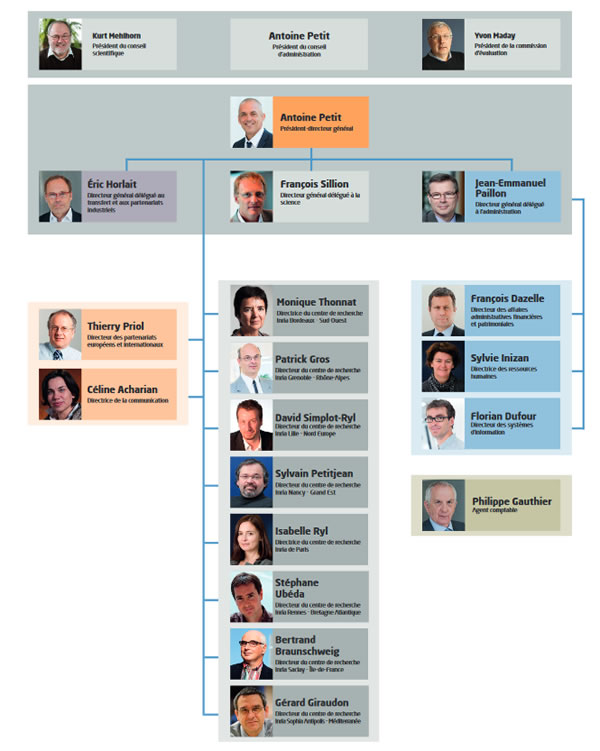
\includegraphics[width=11cm]{Images/organigramme-inria-2016.jpg}
\end{center}

\section{Quelques chiffres}

Le budget primitif d'Inria pour l'ann\'ee 2015 est de
230\,M\euro{}, dont 27\,\% de ressources propres (contrats de recherche
et produits de valorisation). Sur les 4400 personnes (approximativement) pr\'esentes aujourd'hui \`a
Inria, environ 60\% sont des personnels Inria. 
Parmi les titulaires, un tiers sont des chercheurs
et deux tiers des ing\'enieurs, techniciens et administratifs. 

R\'epartis au sein d'environ 230 \'equipes-projets, 
plus de 3400 scientifiques, toutes disciplines confondues,
travaillent \`a l'institut, 
dont environ 1400 chercheur$\cdot$ses et enseignant$\cdot$es-chercheur$\cdot$ses, 
1300 doctorant$\cdot$es et 800 contractuel$\cdot$les
(post-doctorant$\cdot$es, ing\'enieur$\cdot$es expert$\cdot$es et ing\'enieur$\cdot$es associ\'e$\cdot$es).

\liens{panorama.inria.fr/chiffres-cles/}

\section{Les \'equipes-projets de recherche}
\label{sec. projets INRIA}
\index{Equipes-projets Inria (EPI)}

Les \'equipes-projet Inria (EPI) r\'eunissent, autour d'une personnalit\'e scientifique, un groupe de chercheur$\cdot$ses, d'enseignant$\cdot$es chercheur$\cdot$ses, de doctorant$\cdot$es et d'ing\'enieur$\cdot$es. Elles ont toutes un objectif commun : relever un d\'efi scientifique et technologique dans l'un des domaines de recherche prioritaires de l'institut d\'efinis dans le plan strat\'egique.


Pour obtenir le label ``EPI'', le projet de l'\'equipe de recherche doit \^etre approuv\'e par une commission d'\'evaluation comp\'etente dans son domaine scientifique. Une fois labellis\'ee, l'EPI a quatre ans pour mener \`a bien son programme de recherche et atteindre ses objectifs. Pour ce faire, elle dispose de ressources propres. Au terme de quatre ann\'ees, l'EPI fait \`a nouveau l'objet d'une \'evaluation scientifique. Elle peut ainsi \^etre prorog\'ee ou bien arr\^et\'ee. Reconduite deux fois tout au plus, l'EPI a une dur\'ee maximale de vie de 12 ans et une dur\'ee moyenne de 8 ans.

\subsection*{L'\'evaluation des \'equipes-projets}
\index{Evaluation ! \`a l'INRIA}

Toutes les \'equipes-projets d'un m\^eme \textsl{th\`eme} sont
\'evalu\'ees simultan\'ement, de mani\`ere \`a rendre possible les
comparaisons, et \`a permettre de d\'egager une vision globale de la
politique d'Inria sur ce th\`eme. Un groupe d'une dizaine
d'expert$\cdot$es ext\'erieur$\cdot$es, issu$\cdot$es de la communaut\'e scientifique et de
l'industrie, examine les rapports d'activit\'e et les publications
\'emanant des EPI concern\'ees, ainsi que des documents d\'ecrivant
la politique d'Inria et les crit\`eres d'\'evaluation propos\'es.
Depuis 2002, cette \'evaluation se d\'eroule en anglais, ce qui a
permis d'\'elargir consid\'erablement le bassin d'\'evaluateurs
potentiels. Le rapport, qui est r\'edig\'e sans la moindre
interf\'erence de la direction d'Inria, comporte \`a la fois une
analyse globale du th\`eme et des recommandations d\'etaill\'ees
concernant chaque EPI.

Les chefs d'\'equipes-projets r\'edigent ensuite des r\'eponses qui sont
examin\'ees en comit\'e des projets, puis au niveau de la commission
d'\'evaluation. La commission d'\'evaluation r\'edige \`a son tour
des recommandations au$\cdot$\`a la Pr\'esident$\cdot$e d'Inria qui consulte le
conseil scientifique. Le rapport d'\'evaluation externe et l'avis
du conseil scientifique ont en fait un impact durable sur la
strat\'egie de l'institut.

\`A l'issue de tout ce processus, une d\'ecision formelle est sign\'ee
par la ou le Pr\'esident$\cdot$e Directeur$\cdot$trice G\'en\'eral$\cdot$e qui autorise la poursuite
de l'\'equipe-projet, ou demande son arr\^et. Lorsqu'une EPI s'arr\^ete, les
chercheuses et chercheurs ont le temps de r\'efl\'echir pour savoir s'ils
souhaitent rejoindre une autre EPI, ou proposer de nouveaux
objectifs pour cr\'eer une nouvelle EPI, en suivant les conseils du
directeur de l'unit\'e et du pr\'esident du comit\'e des projets.

\section{La commission d'\'evaluation}
\index{Commission d'\'evaluation INRIA}
\index{Evaluation ! \`a l'INRIA}

La commission d'\'evaluation d'Inria, dot\'ee d'une forte autonomie, est au c{\oe}ur de l'\'evaluation scientifique de l'Institut. Elle est compos\'ee de personnalit\'es scientifiques \'elues et nomm\'ees d'Inria et d'expert$\cdot$es ext\'erieur$\cdot$es \`a l'Institut. En liaison avec la Direction des recherches, elle coordonne l'\'evaluation externe du travail des \'equipes-projets Inria, domaine de recherche par domaine de recherche. Elle forme le c\oe ur des jurys d'admissibilit\'e des concours qui contiennent aussi des personnalit\'es ext\'erieures nomm\'ees par la Direction g\'en\'erale, ainsi que les commissions proposant les promotions internes. Elle intervient enfin dans l'\'evaluation de la cr\'eation des projets et dans celle des actions scientifiques collectives d'Inria.

Dans le cadre de ses missions, la commission d'\'evaluation constitue des groupes de travail sur des sujets li\'es \`a l'\'evaluation (exemples : parit\'e homme-femme, \'evaluation des logiciels, du transfert technologique, de la diffusion scientifique, {\it etc}). Elle m\`ene \'egalement des r\'eflexions de nature strat\'egique sur l'\'evolution des domaines scientifiques d'Inria et l'\'evolution associ\'ee du m\'etier de chercheur.

La commission d'\'evaluation compte 40 membres au total :
\begin{itemize}
\item 20 membres nomm\'es par le$\cdot$la pr\'esident$\cdot$e de l'institut dont 10 sur proposition du ou de la pr\'esident$\cdot$e du conseil scientifique~;
\item 20 membres \'elus par et parmi le personnel de l'\'etablissement, selon des modalit\'es fix\'ees
par d\'ecision de la ou du pr\'esident$\cdot$e de l'institut.
\end{itemize}
Les membres nomm\'es sont choisis, pour la moiti\'e d'entre eux, parmi les personnalit\'es scientifiques
ext\'erieures \`a l'institut. Le$\cdot$La pr\'esident$\cdot$e de cette commission est d\'esign\'e$\cdot$e parmi ses membres par le$\cdot$la
 pr\'esident$\cdot$e de l'institut, sur proposition du$\cdot$de la pr\'esident$\cdot$e du conseil scientifique.  
 
\liens{www.inria.fr/institut/organisation/instances/commission-d-evaluation}

 
%%%%%%%%%%%%%%%%%%%%%%%%%%%%%%%%%%%%%%%%%%%%%%%%%%
 
 \chapter{INRAE}
 
 \section{Structure et fonctionnement}
 
L'Institut National de Recherche pour l'Agriculture, l'alimentation et l'Environnement (INRAE), issu de la fusion au 1er janvier 2020 entre l'Institut national de Recherche en Sciences et Technologies pour l'Environnement et l'Agriculture (IRSTEA) et de l’Institut National de la Recherche Agronomique (INRA), est un organisme de recherche qui mobilise de nombreuses disciplines scientifiques r\'eparties dans 14 d\'epartements scientifiques de recherche\footnote{
\og Action, transition et territoires \fg{},
\og  Agro\'ecosyst\`emes \fg{},
\og  Alimentation Humaine \fg{},
\og  Aliments, produis biosourc\'es et d\'echets \fg{},
\og  Biologie et am\'elioration des Plantes \fg{},
\og  \'Ecologie et biodiversit\'e \fg{},
\og  \'Economie et sciences sociales \fg{},
\og  \'Ecosyst\`emes aquatiques, ressources en eau et risques \fg{},
\og  G\'en\'etique Animale \fg{},
\og  Math\'ematiques et num\'erique \fg{},
\og  Microbiologie et cha\^ine alimentaire \fg{},
\og  Physiologie animale et syst\`emes d'\'elevage \fg{},
\og  Sant\'e animale \fg{},
\og  Sant\'e des plantes et environnement \fg{}.}.
Ces d\'epartements se r\'epartissent sur 18 centres sur toute la France et regroupe un peu plus de 200 unit\'es de recherche.

\textbf{Lien utile\hspace{.5em}}\url{https://www.inrae.fr}

\section{Le d\'epartement MathNum} 

Le d\'epartement MathNum m\`ene des recherches en math\'ematique et en sciences et technologies du num\'erique (informatique, bioinformatique et intelligence artificielle, en sciences de l'information et de la communication, sur les technologies de robotiques, capteurs et imagerie satellitaire). Il se distingue par sa position transversale et collabore r\'eguli\`erement avec d'autres d\'epartements d'INRAE, ainsi qu'avec des partenaires scientifiques nationaux et internationaux tels qu'INRIA, le CNRS, des universit\'es et des grandes \'ecoles Paris-Saclay, AgroParisTech, Montpellier, Toulouse,  {\em etc}). Grâce \`a ses collaborations interdisciplinaires, le d\'epartement contribue \`a la compr\'ehension, la pr\'ediction et l'aide \`a la d\'ecision sur des syst\`emes complexes relevant des sciences du vivant et de l'environnement

MathNum est impliqu\'e dans des communaut\'es disciplinaires en math\'ematique, informatique, sciences et technologies du num\'erique, sous la forme de Labex, fondations, instituts convergences (DigitAg et Dataia), institut interdisciplinaire en intelligence artificielle (3IA Aniti), f\'ed\'erations ou groupes de recherche.

Exer\c{c}ant nos recherches dans le cadre d’une science ouverte motiv\'ee par l’acquisition des connaissances et sensibles aux grands enjeux soci\'etaux d’aujourd’hui, les \'equipes du D\'epartement partagent l’ambition de d\'evelopper un num\'erique responsable, attentif \`a des enjeux tels que la reproductibilit\'e, l’innovation ouverte, la mesure de l‘impact et la frugalit\'e num\'erique.

\textbf{Lien utile\hspace{.5em}}\url{https://www.inrae.fr/departements/mathnum}

\subsection{Champs th\'ematiques}

Les activit\'es du D\'epartement incluent de la recherche th\'eorique, m\'ethodologique et appliqu\'ee, avec des collaborations notamment en biologie et \'ecologie pr\'edictives, en \'epid\'emiologie, en agriculture num\'erique, et plus g\'en\'eralement pour l’\'etude et la mod\'elisation des syst\`emes complexes rencontr\'es dans les domaines d’int\'er\^et d’INRAE. Les recherches de MathNum s’organisent selon cinq champs th\'ematiques (CT), refl\'etant ses grands domaines de comp\'etence m\'ethodologiques et technologiques par rapport à la gestion de la donn\'ee et au traitement de l’information :
\begin{itemize}
\item Optique et t\'el\'ed\'etection, m\'etrologie, capteurs, traitement du signal ;
\item Repr\'esentation et extraction des connaissances, syst\`emes d'information ;
\item Probabilit\'es, statistique et apprentissage automatique ;
\item Mod\'elisation des syst\`emes complexes et syst\`emes dynamiques ;
\item Technologies pour l'action. automatique et contr\^ole, recherche op\'erationnelle.
\end{itemize}

\textbf{Lien utile\hspace{.5em}}\url{https://www.inrae.fr/departements/mathnum/recherches-du-departement-mathnum}

\subsection{Dispositif de recherche}

Le d\'epartement regroupe 24 \'equipes scientifiques r\'eparties dans 11 unit\'es de recherche sur 7 centres r\'egionaux INRAE. Parmi ces unit\'es de recherche, on compte 4 Unit\'es Mixtes de Recherche (UMR) : MIA Paris - Saclay (avec AgroParisTech), ITAP, MISTEA et TETIS (avec SupAgro \`a Montpellier) et une unit\'e sous contrat \`a Evry avec le CNRS et l'Universit\'e d'Evry.

\textbf{Lien utile\hspace{.5em}}\url{https://www.inrae.fr/departements/mathnum/structures-du-departement-mathnum}

\subsection{Ressources humaines et comp\'etences}

Le d\'epartement MathNum est en taille le plus petit d\'epartement d'INRAE. La population des chercheur\mp euse\mp s du d\'epartement se r\'epartit au sein de trois grandes familles disciplinaires : probabilit\'es et statistique, informatique et syst\`emes dynamiques. En 2023, le d\'epartement comptait pr\`es de 190 titulaires (INRAE ou en accueil) et 160 contractuels dont une centaine de doctorants. 

Toutes les chercheuses et tous les chercheurs du d\'epartement sont \'evalu\'es par la Commission Scientifique Sp\'ecialis\'ee Math\'ematiques, Bio-Informatique, Intelligence Artificielle.

\subsection{Les infrastructures et r\'eseaux de MathNum}

Le Département MathNum est fortement impliqué dans le pilotage d’infrastructures scientifiques d’intérêt collectif.

\textbf{Lien utile\hspace{.5em}}\url{https://www.inrae.fr/departements/mathnum/infrastructures-reseaux-mathnum}



%\section{ Le d\'epartement de Math\'ematiques et Informatique Appliqu\'ees}
%Le d\'epartement Math\'ematiques et Informatique Appliqu\'ees (MIA, \lien{www.mia.inra.fr/ } ou\\  \lien{www.mathinfo.inra.fr/fr} ) partage avec les autres d\'epartements de recherche de l'INRAE la mission principale de production de connaissances g\'en\'eriques et finalis\'ees, de mise au point de m\'ethodes, d'outils et de savoir-faire, dans ses champs de comp\'etences que sont les math\'ematiques et l'informatique appliqu\'ees aux domaines de l'alimentation, l'agriculture et l'environnement. \\
%L'emploi des math\'ematiques et de l'informatique est aujourd'hui fondamental pour relever les d\'efis scientifiques et technologiques auxquels fait face la recherche agronomique et les besoins en comp\'etences en math-info (m\'ethodes et ing\'enierie) augmentent dans tous les domaines de l'INRAE et ne se limitent plus au p\'erim\`etre du d\'epartement MIA. Ce nouveau contexte a ainsi conduit \`a actualiser r\'ecemment le r\^ole du d\'epartement MIA au sein de l'institut \`a travers trois familles de missions:
%\begin{itemize}
%\item Mission I : Le d\'epartement a pour mission de mener des recherches en math-info sur des verrous m\'ethodologiques qui \'emergent des enjeux prioritaires de la recherche agronomique (sciences du vivant, de l'environnement, etc.), et de mettre en oeuvre ces recherches via des partenariats (projets, th\`eses, etc.).
%\item Mission II : Le d\'epartement a \'egalement pour mission de conduire dans un cadre inter-disciplinaire des recherche \`a l'interface sur des enjeux prioritaires de l'INRAE pour lesquels le r\^ole des math-info, nouveau ou g\'en\'erique, est incontournable.
%\item Mission III : Le d\'epartement a enfin pour mission d'accompagner le d\'eveloppement des math\'ematiques et informatique \`a l'INRAE, concernant en particulier : 
%\begin{itemize}
%\item[(i)] l'ing\'enierie du dispositif INRAE en mati\`ere de traitement, gestion et analyse de donn\'ees, de calcul et de simulation, en particulier dans le cadre de plates-formes ;
%\item[(ii)] l'expertise en m\'ethodologie math\'ematiques-informatique et en ing\'enierie informatique et calcul intensif en direction des d\'epartements et des programmes ;
%\item[(iii)] la formation, l'entretien de la comp\'etence m\'etier, la diffusion et la promotion de la culture math\'e\-matiques-informatique ; 
%\item[(iv)] le suivi des partenariats entre l'INRAE et les autres organismes concernant les math\'ematiques et l'informatique.
%\end{itemize}
%\end{itemize}
%En termes m\'ethodologiques, les priorit\'es du d\'epartement MIA se d\'eclinent \`a l'heure actuelle selon deux axes li\'es \`a la gestion et \`a l'analyse des masses de donn\'ees h\'et\'erog\`enes et \`a la construction, analyse et simulation de mod\`eles complexes.
%
%\subsection{ Dispositif de recherche}
%
% Le d\'epartement MIA pilote ou co-pilote 7 unit\'es de recherche, pr\'esentes sur six sites INRAE en m\'etropole : trois sont des unit\'es dites "propres" et constitu\'ees quasi-exclusivement de   personnes rattach\'ees \`a MIA (MIA Toulouse \lien{carlit.toulouse.inra.fr/wikiz/index.php/Accueil} , MIA Jouy \\  \lien{www6.jouy.inra.fr/mia} et BioSP \lien{www.biosp.org/} en Avignon) une unit\'e, MIG\\ \lien{mig.jouy.inra.fr/ } \`a Jouy-en-Josas, est commune avec les d\'epartements PHASE et MICA , et deux unit\'es sont des Unit\'es Mixtes de Recherche (UMR) avec d'autres organismes de recherche ou d'enseignement (l'unit\'e MISTEA de Montpellier \lien{www6.montpellier.inra.fr/mistea/}  avec l'\'ecole SupAgro et l'INRIA et l'unit\'e MIA de Paris \lien{www.agroparistech.fr/mia/ } avec l'\'ecole AgroParisTech. Enfin, le d\'epartement MIA est impliqu\'e dans une unit\'e sous contrat \`a Evry avec le CNRS et l'Universit\'e d'Evry (\lien{www.math-evry.cnrs.fr/sg/welcome}).

%\subsection{Les r\'eseaux scientifiques soutenus par le d\'epartement MIA}
%Le d\'epartement soutient fortement plusieurs r\'eseaux scientifiques sur des th\'ematiques vari\'ees : Elicitations de dires d'experts, Algorithmic Issues for Inference in Graphical Models (AIGM), Exploration num\'erique des propri\'et\'es des mod\`eles (MEXICO), Inf\'erence de R\'eseaux Biologiques (NETBIO), Mod\'elisation de paysage agricole (PAYOTE), Taxonomie num\'erique mol\'eculaire (TANUMO), Mod\'elisation et statistique en sant\'e des animaux et des plantes (ModStatSAP), Statistique pour les trajectoires, Int\'egration de sources/masses de donn\'ees h\'et\'erog\`enes et ontologies, Statistiques pour les Sciences Participatives (CiSStats), Mod\'elisation et simulation informatique des agro-\'ecosyst\`emes (RECORD), formalisme Discrete Event System (DEVS), Mod\`eles et M\'ethodes statistiques pour les variables spatio-temporelles, Syst\`emes d'\'equations diff\'erentielles et autres syst\`emes dynamiques pour l'\'ecologie (MEDIA), R\'eduction et simplification de mod\`eles (REM), Optimisation : m\'ethodes et applications dans les sciences de la vie.

%%%%%%%%%%%%%%%%%%%%%%%%%%%%%%%%%%%%%%%%%%%%%%%%%
%%%%%%%%%%%%%%%%%%%%%%%%%%%%%%%%%%%%%%%%%%%%%%%%%

\chapter[HCERES]{HCERES} \label{HCERES}

\index{Haut Conseil de l'\'Evaluation de la Recherche et de l'Enseignement Sup\'erieur (HCERES)}

Cr\'e\'e par la \href{https://www.legifrance.gouv.fr/loda/id/JORFTEXT000027735009}{loi n°2013-660 du 22 juillet 2013 relative \`a l'Enseignement Sup\'erieur et \`a la Recherche} (ESR), le Haut Conseil de l'\'evaluation de la recherche et de l'enseignement sup\'erieur (HCERES) succ\`ede \`a l'Agence d'\'evaluation de la recherche et de l'enseignement sup\'erieur (AERES). Ce conseil est la {\em seule} autorit\'e administrative fran\c caise
charg\'ee de l'\'evaluation de l'enseignement sup\'erieur et de la recherche publics.
Le HCERES a pour vocation de rassembler sous un m\^eme toit les ex-MSTP, ex-CNE
et ex-CNER\footnote{%
MSTP~: Mission scientifique, technique et p\'edagogique~;
CNE~: Comit\'e national d'\'evaluation
des \'etablissements publics \`a caract\`ere scientifique, culturel et
professionnel~;
CNER~: Comit\'e national d'\'evaluation de la recherche},
et d'assurer les missions d'\'evaluation des EPCSCP (donc les universit\'es), des EPST (donc le CNRS, INRIA, INRAE),
leur recherche (donc les laboratoires) et leur formation. Le HCERES \textbf{ne fait pas d'\'evaluations individuelles}. Les enseignant\mp e\mp s-chercheur\mp euse\mp s sont évalués par le Conseil National des Universit\'es (CNU, {\em cf.}, Chapitre \ref{CNU}). 

On rappelle que les \'equipes INRIA ne sont pas \'evalu\'ees par le HCERES, c'est l'\'etablissemnt qui est \'evalu\'e. 
Les \'equipes sont \'evalu\'ees suivant une proc\'edure propre \`a INRIA ({\em cf.}, Chapitre \ref{INRIA}). 

\textbf{Lien utile\hspace{0.5em}}\url{https://www.hceres.fr}


%%%%%%%%%%%%%%%%%%%%%%%%%%%%%%%%%%%%%%%%%%%
\section{Statut, missions et organisation}

Le HCERES est une autorit\'e administrative ind\'ependante. 
Pour l'exercice de ses missions, il s'inspire des meilleures pratiques internationales. Il fonde son action, en ce qui concerne les crit\`eres d'\'evaluation, sur les principes d'objectivit\'e, 
de transparence et d'\'egalit\'e de traitement entre les structures examin\'ees et, en ce qui concerne le choix des personnes charg\'ees de l'\'evaluation, sur les principes d'expertise scientifique au meilleur niveau international, 
de neutralit\'e et d'\'equilibre dans la repr\'esentation des th\'ematiques et des opinions. Il veille \`a la pr\'evention des conflits d'int\'er\^ets dans la constitution des comit\'es d'expert\mp e\mp s charg\'e\mp e\mp s de conduire les \'evaluations. 
Il peut conduire directement des \'evaluations ou s'assurer de la qualit\'e des \'evaluations r\'ealis\'ees par d'autres instances en validant les proc\'edures retenues. Il met en mesure les structures et \'etablissements qu'il \'evalue directement de pr\'esenter, 
\`a leur demande, des observations tout au long et \`a l'issue de la proc\'edure d'\'evaluation.

Le HCERES est charg\'e:
\begin{itemize}
\item d'\'evaluer les \'etablissements d'enseignement sup\'erieur et leurs regroupements, les organismes de recherche, les fondations de coop\'eration scientifique et l'Agence nationale de la recherche ou, le cas \'ech\'eant, de s'assurer de la qualit\'e des \'evaluations conduites par d'autres instances ;
\item d'\'evaluer les unit\'es de recherche \`a la demande de l'\'etablissement dont elles rel\`event, en l'absence de validation des proc\'edures d'\'evaluation ou en l'absence de d\'ecision de l'\'etablissement dont rel\`event ces unit\'es de recourir \`a une autre instance ou, le cas \'ech\'eant, 
de valider les proc\'edures d'\'evaluation des unit\'es de recherche par d'autres instances.
\end{itemize}

Lorsqu'une unit\'e rel\`eve de plusieurs \'etablissements, il n'est proc\'ed\'e qu'\`a une seule \'evaluation. 
Lorsque les \'etablissements d\'ecident conjointement de recourir \`a une autre instance, le Haut Conseil valide les proc\'edures d'\'evaluation mises en \oe uvre par cette instance. Dans le cas contraire, le Haut Conseil \'evalue l'unit\'e de recherche,
\begin{itemize}
\item en \'evaluant les formations et dipl\^omes des \'etablissements d'enseignement sup\'erieur ou, le cas \'ech\'eant, 
en validant les proc\'edures d'\'evaluation r\'ealis\'ees par d'autres instances.
\item en s'assurant de la prise en compte, dans les \'evaluations des personnels de l'enseignement sup\'erieur et de la recherche, de l'ensemble des missions qui leur sont assign\'ees par la loi et leurs statuts particuliers ;
\item en s'assurant de la valorisation des activit\'es de diffusion de la culture scientifique, technique et industrielle dans la carri\`ere des personnels de l'enseignement sup\'erieur et de la recherche ;
\item en \'evaluant a posteriori les programmes d'investissement et les structures de droit priv\'e recevant des fonds publics destin\'es \`a la recherche ou \`a l'enseignement sup\'erieur. 
\end{itemize}
Dans le cadre de programmes de coop\'eration europ\'eens ou internationaux ou \`a la demande des autorit\'es comp\'etentes, le HCERES peut participer \`a l'\'evaluation d'organismes \'etrangers ou internationaux de recherche et d'enseignement sup\'erieur.
Le Haut Conseil comporte \'egalement un Observatoire des Sciences et Techniques (OST) charg\'e de conduire des \'etudes et analyses strat\'egiques. 

Les campagnes \'evaluations suivent un rythme quinquennal et se font \textit{par vagues}: A, B, C, D ou E.
Le Haut Conseil a ainsi d\'efini un cycle de campagnes d'\'evaluation calqu\'ees sur cette r\'epartition \textit{par vagues}.
Tous les ans, il \'evalue les \'etablissements d'une même \textit{vague}.

\textbf{Lien utile\hspace{.5em}}\url{https://www.hceres.fr/fr/les-campagnes-devaluation}


%Le HCERES est une autorit\'e administrative ind\'ependante charg\'ee
%d'\'evaluer
%les \'etablissements et organismes de recherche (et
%d'enseignement sup\'erieur, le cas \'ech\'eant), ainsi que leurs
%activit\'es de recherche. Elle est \'egalement charg\'ee de
%l'\'evaluation de l'ANR et des formations et dipl\^omes de
%l'enseignement sup\'erieur. En ce qui concerne l'\'evaluation des
%{\em individus}, le HCERES n'est charg\'ee que de valider les
%proc\'edures men\'ees soit par le CNU (dans les universit\'es), soit
%par le Comit\'e National (pour les chercheurs CNRS) ; nous renvoyons
%pour cela aux sections suivantes. Il est \`a noter qu'INRIA \'evalue ses
%\'equipes-projets, mais ne pratique pas d'\'evaluation individuelle,
%sauf lors d'une mutation et/ou d'une promotion, voir les sections \ref{CE-INRIA}
%et \ref{sec. projets INRIA}.
%
%\medskip
%
%Le HCERES est organis\'ee en trois sections correspondant \`a ses principales missions~:
%
%\begin{itemize}
%
%\item La {\em section des \'etablissements} est comp\'etente, d'une part, pour
%\'evaluer les \'etablissements et organismes li\'es \`a la recherche et,
%d'autre part, pour valider les proc\'edures d'\'evaluation de leurs
%personnels, et pr\'eparer un avis
%sur les conditions dans lesquelles elles sont mises en \oe uvre.
%
%\item La {\em section des unit\'es de recherche} est comp\'etente pour l'\'evaluation des
%activit\'es des unit\'es de recherche des \'etablissements et organismes
%li\'es \`a la recherche. Elle conduit l'\'evaluation soit directement,
%soit en s'appuyant sur les \'etablissements et organismes selon
%des proc\'edures qu'elle a valid\'ees.
%
%\item La {\em section des formations} est comp\'etente pour l'\'evaluation des
%formations et des dipl\^omes (licence, master).
%\end{itemize}
%
%\medskip
%
%Chaque {section} est dirig\'ee par un directeur nomm\'e pour un mandat de quatre ans renouvelable
% par le conseil de l'agence sur proposition du pr\'esident de l'agence. Aux c\^ot\'es de ces sections, si\`ege
% ledit {conseil}, compos\'e de 25 membres renouvel\'es par moiti\'e tous les deux ans, nomm\'es par
% diff\'erentes instances (minist\`ere, organismes de recherche, CNU, comit\'e national, parlement). Chaque
% \'evaluation est conduite par un {comit\'e d'\'evaluation}, dont les membres sont choisis par le pr\'esident
% de la section concern\'ee, apr\`es avis et propositions du conseil, des pr\'esidents ou directeurs des
%\'etablissement d'ESR, des chefs d'instances d'\'evaluation nationale.\\

\bigskip

Le HCERES est administr\'e par un coll\`ege garant de la qualit\'e de ses travaux. Le coll\`ege arr\^ete le programme annuel d'\'evaluation du Haut Conseil. Il d\'efinit les mesures propres \`a garantir la qualit\'e, la transparence et la publicit\'e des proc\'edures d'\'evaluation. Son\mp sa Pr\'esident\mp e, nomm\'e\mp e parmi ses membres, dirige le Haut Conseil et a autorit\'e sur ses personnels. Le coll\`ege est compos\'e de trente membres nomm\'es par d\'ecret pour une dur\'ee de quatre ans, renouvelable une fois.

Le coll\`ege comprend :
\begin{itemize}
\item Neuf membres ayant la qualit\'e de chercheur\mp euse, d'ing\'enieur\mp e ou d'enseignant\mp e-chercheur\mp euse, nomm\'e\mp e\mp s sur proposition des instances d'\'evaluation comp\'etentes en mati\`ere d'enseignement sup\'erieur et de recherche parmi leurs membres \'elu\mp e\mp s, dont au moins trois sur proposition de l'instance nationale mentionn\'ee 
\`a l'article L. 952-6 du code de l'\'education et au moins trois sur proposition des instances d'\'evaluation mentionn\'ees \`a l'article L. 321-2 du pr\'esent code ;
\item Huit membres ayant la qualit\'e de chercheur\mp euse, d'ing\'enieur\mp e ou d'enseignant\mp e-chercheur\mp euse, dont trois sur proposition des pr\'esident\mp e\mp s ou directeur\mp ices d'organismes de recherche et trois sur proposition des conf\'erences des chefs d'\'etablissements mentionn\'ees \`a l'article L. 233-1 du code de l'\'education ;
\item Deux membres repr\'esentant les \'etudiant\mp e\mp s, sur proposition des associations d'\'etudiant\mp e\mp s en fonction du nombre de voix obtenues par ces associations lors de l'\'election des repr\'esentants des \'etudiant\mp e\mp s au Conseil national de l'enseignement sup\'erieur et de la recherche ;
\item Neuf personnalit\'es qualifi\'ees, fran\c caises et \'etrang\`eres, dont au moins trois issues du secteur de la recherche priv\'ee et trois appartenant \`a des agences d'accr\'editation ou d'\'evaluation \'etrang\`eres ;
\item Un\mp e d\'eput\'e\mp e et un\mp e s\'enateur\mp ice d\'esign\'e\mp e\mp s par la commission permanente comp\'etente en mati\`ere d'enseignement sup\'erieur et de recherche de chaque assembl\'ee.
\end{itemize}
 
\textbf{Lien utile\hspace{.5em}}\url{https://www.hceres.fr/fr/college-du-hceres}


%Voici l'organigramme qu'on peut trouver sur le site du HCERES :
%
%\begin{center}
%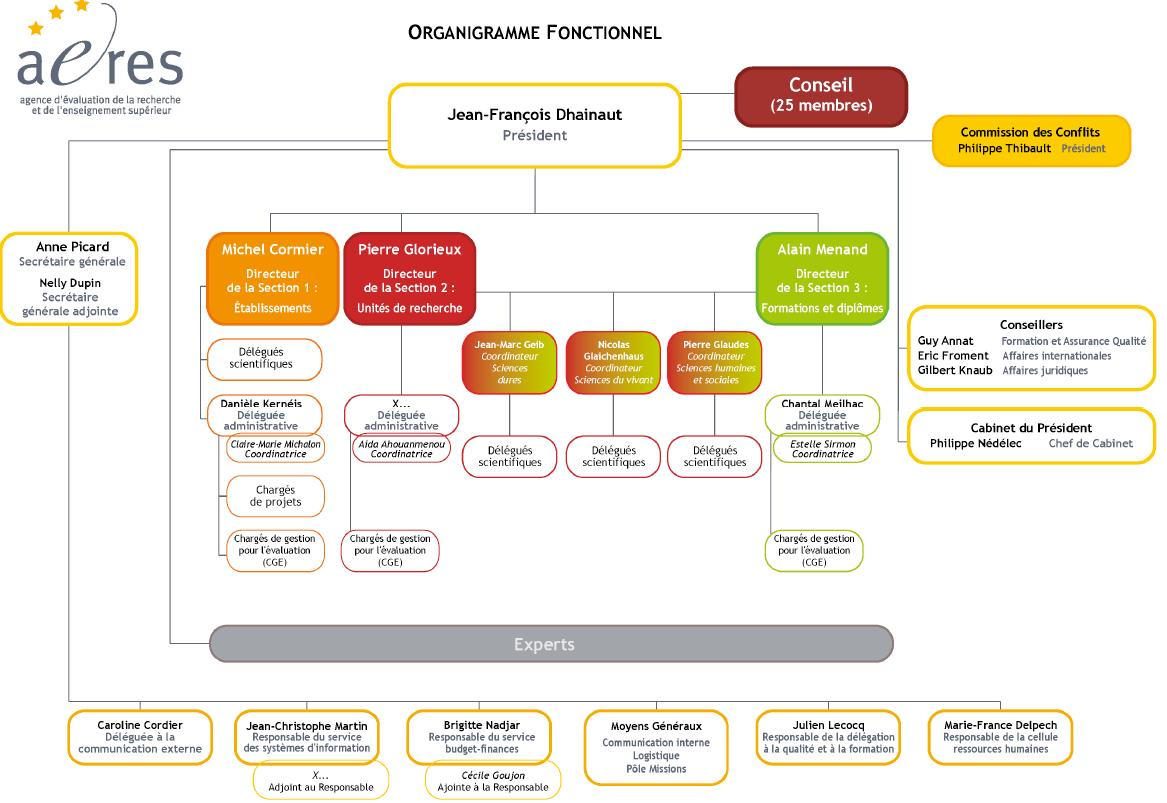
\includegraphics[width=12cm]{organigramme_aeres.jpg}
%\end{center}
%
%Il est \`a noter que le point le plus critiqu\'e par la communaut\'e scientifique sur le fonctionnement de
% l'AERES est le fait que \textit{tous} les membres soient \textit{nomm\'es}, ce qui peut \^etre
%consid\'er\'e en contradiction avec l'objectif d'ind\'ependance affich\'e par la loi.\\
%
%Le d\'ecret relatif \`a la mise en place de l'agence est disponible sur
%le site du Journal Officiel.\\
%\lien{www.legifrance.gouv.fr/WAspad/UnTexteDeJorf?numjo=MENX0600140D}\\



%\section{Les crit\`eres d'\'evaluation}
%
%Les crit\`eres d'\'evaluation des \'etablissements ne sont pas pr\'ecis\'es par les textes
%instaurant le HCERES, et sont donc laiss\'es \`a l'appr\'eciation des comit\'es d'\'evaluation
% (\`a l'exception de la valorisation des recherches, explicitement cit\'ee par la loi).
%
%\textbf{Lien utile\hspace{.5em}}\url{https://www.hceres.fr/fr/referentiels-devaluation}

\section{L'\'evaluation des laboratoires}
\index{Evaluation ! des laboratoires}

La section des unit\'es r\'ealise plus de 700 \'evaluations par an
(chaque unit\'e \'etant \'evalu\'ee tous les cinq ans) sur la base d'un dossier scientifique
remis par l'unit\'e et de visites sur site par un comit\'e d'experts.
Il s'agit d'une \'evaluation transparente et contradictoire,
ax\'ee sur un rapport d'expertise et une notation.
Les rapports d'\'evaluation sont publics et accessibles sur le site internet de l'agence.

\textbf{Lien utile\hspace{.5em}}\url{https://www.hceres.fr/fr/les-rapports-et-syntheses}
 
 Les crit\`eres d'\'evaluation des \'etablissements ne sont pas pr\'ecis\'es par les textes
instaurant le HCERES, et sont donc laiss\'es \`a l'appr\'eciation des comit\'es d'\'evaluation
 (\`a l'exception de la valorisation des recherches, explicitement cit\'ee par la loi). On
peut trouver sur le site du HCERES les grilles d'\'evaluation qui seront
remplies par les expert\mp e\mp s, ce qui permet de se faire une id\'ee des
crit\`eres d'\'evaluation~: outre un profil quantitatif (indiquant
notamment la taille des \'equipes, le nombre de publiant\mp e\mp s ou le
nombre de th\`eses en cours et soutenues), y figure \'egalement un
profil qualitatif dans lequel apparaissent l'originalit\'e et
l'int\'er\^et des recherches, le niveau et la notori\'et\'e des
travaux, {\em etc}.

\textbf{Lien utile\hspace{.5em}}\url{https://www.hceres.fr/fr/referentiels-devaluation}

En pratique, lorsque son \'etablissement d'appartenance est \'evalu\'e, le laboratoire
doit constituer un dossier, qui est sous la responsabilit\'e de la directrice ou du directeur du laboratoire.
Ce dossier contient un rapport
d'activit\'e global du laboratoire, la liste des publications pendant
la p\'eriode de contractualisation finissante, le programme de
recherche pour les cinq ann\'ees \`a venir, \`a l'\'echelle du
laboratoire, et les ressources financi\`eres demand\'ees
pour mener \`a bien ce programme de recherche.


\section{Accr\'editation des \'etablissements d'enseignement sup\'erieur}
\index{Accr\'editation}
\index{Conseil National de l'Enseignement Sup\'erieur et de la Recherche (CNESER)}

Depuis la loi ESR de 2013, les \'etablissements ne demandent plus au minist\`ere l'habilitation des formations, 
mais demandent l'accr\'editation pour l'ensemble de leurs formations. Le HCERES s'assure que les formations respectent 
le cadre national d\'efini par le CNESER ({\em cf.}, Section \ref{CNESER}). Il veille également à ce que les \'etablissement 
assurent la qualit\'e  de la formation en l'adossant aux activit\'es de recherche, et en suivant les \'etudiant\mp e\mp s dans leurs parcours. Aussi sur la base de l'\'evaluation HCERES, la DGESIP ({\em cf.}, Section \ref{DGESIP}) du minist\`ere d\'ecide de l'accr\'editation pour la dur\'ee de cinq ann\'ees.

\textbf{Lien utile\hspace{.5em}}
\href{https://www.legifrance.gouv.fr/affichTexte.do?cidTexte=JORFTEXT000028543620&categorieLien=id}{Arrêt\'e du 22 janvier 2014 fixant les modalit\'es d'accr\'editation d'\'etablissements d'enseignement sup\'erieur}


%%%%%%%%%%%%%%%%%%%%%%%%%%%%%%%%%%%%%%%%%%%
%%%%%%%%%%%%%%%%%%%%%%%%%%%%%%%%%%%%%%%%%%%

\chapter{Le CNU} \label{CNU}


Le conseil national des
universit\'es (CNU) est l'instance nationale comp\'etente pour le
recrutement et la carri\`ere des enseignant$\cdot$es-chercheur$\cdot$ses.
Il est en particulier charg\'e d'examiner les demandes de
qualification (MCF et PR), de promotion, et de cong\'e pour
recherche ou conversion th\'ematique (CRCT). 
Depuis 2014, il est charg\'e d'\'emettre un avis sur les demandes de PEDR et bient\^ot, il pourrait \'egalement \^etre en charge d'effectuer le suivi de carri\`ere des enseignant$\cdot$es-chercheur$\cdot$ses.

\index{Conseil national des universit\'es (CNU)}
\index{Cong\'e pour recherche ou conversion th\'e\-ma\-ti\-que
(CRCT)}
\index{Professeur d'universit\'e (PR)!qualification aux fonctions
de}
\index{Ma\^\i tre de conf\'erences (MCF)!qualification aux fonctions de}

%%%%%%%%%%%%%%%%%%%%%%%%%%%%%%%%%%%%%%
\section{Sa composition}

En 25\ieme{} (math\'ematiques) et 26\ieme{}
(math\'ematiques appliqu\'ees et
applications des math\'e\-ma\-ti\-ques) sections, le CNU est
compos\'e de 96 membres~: 48 titulaires et 48 suppl\'eant$\cdot$es, les rangs A (PR
et assimil\'es) et rangs B (MCF et assimil\'es) \'etant
repr\'esent\'es \`a parit\'e. %Les membres nomm\'es le sont par le minist\`ere. 
Chaque conseil si\`ege pour quatre ans et poss\`ede un
bureau constitu\'e de six personnes~: un$\cdot$e pr\'esident$\cdot$e (PR), deux
vice-pr\'esident$\cdot$es (un PR et un MCF) et trois assesseurs (1 PR et 2 MCF). Vous
trouverez la composition actuelle des CNU 25 et 26 sur les sites\\
\lien{cnu25.emath.fr/} et \lien{cnu26.emath.fr/}.

\index{Professeur$\cdot$e d'universit\'e (PR)} \index{Ma\^\i tre de
conf\'erences (MCF)}
%%%%%%%%%%%%%%%%%%%%%%%%%%%%%%%%%%%%%%%%%
\section{Ses missions}
\subsection{La qualification} \label{kalif}

La qualification est une des \'etapes n\'ecessaires pour postuler (voir \ref{recrutement})
aux fonctions de ma\^\i  tre de conf\'erences ou de professeur$\cdot$e des
universit\'es (sauf pour les postes r\'eserv\'es aux MCF habilit\'e$\cdot$es
ayant plus de dix ans d'anciennet\'e). Le nombre de qualifi\'e$\cdot$es
n'est pas li\'e au nombre de postes offerts au concours. La
qualification reste valable quatre ans et, chaque ann\'ee, un
arr\^et\'e pr\'ecise les modalit\'es et les conditions d'inscription
sur la liste de qualification.  Un lien vers ces arr\^et\'es peut \^etre trouv\'e \`a l'adresse\\
\lien{cnu25.emath.fr/qualif/index.html}. \\

La proc\'edure est la suivante (les dates sont donn\'ees \`a titre
indicatif)~:
\begin{itemize}

\item septembre/octobre~: inscription sur les listes de demande
de qualification. L'inscription se fait sur l'application ANTARES.
Vous obtenez ainsi un num\'ero de candidat$\cdot$e (indispensable).
Attention~: la cl\^oture des inscriptions est d\'efinitive~! Si vous
ratez cette \'etape, il vous faut attendre l'ann\'ee suivante~;

\index{ANTARES}

\item novembre/d\'ecembre~: d\'esignation par le bureau du CNU des
rapporteurs (2 par candidat$\cdot$e) ;
\item mi-d\'ecembre~: date \`a laquelle la th\`ese ou l'habilitation doit avoir \'et\'e soutenue~;
\item mi-d\'ecembre~: envoi des dossiers aux
rapporteur$\cdot$trices. Les titulaires de dipl\^omes
universitaires, qualifications et titres de niveau \'equivalent
peuvent \^etre dispens\'e$\cdot$es du doctorat (ou de l'habilitation) par le
CNU. Dans la pratique, cette dispense peut \^etre accord\'ee pour
les candidat$\cdot$es ayant effectu\'e leurs \'etudes et/ou une partie de
leur carri\`ere \`a l'\'etranger~;

\index{Habilitation \`a diriger des recherches (HDR)}

\item janvier/f\'evrier~: examen des dossiers~;

\item janvier/f\'evrier~: r\'eunion et d\'ecisions du CNU. Lors de
cette r\'eunion, le dossier de chaque candidat$\cdot$e est d\'ecrit par les
rapporteur$\cdot$trices et l'ensemble des membres du CNU d\'ecide de la
qualification. Seuls les rangs A du CNU examinent et d\'ecident des
qualifications aux fonctions de professeur$\cdot$e~;

\item f\'evrier~: les candidat$\cdot$es consultent leurs r\'esultats sur ANTARES et impriment l'\'ecran pour en conserver une copie.\\
\end{itemize}

En cas de refus de qualification, la ou le candidat$\cdot$e peut demander les
rapports \'ecrits des deux rapporteur$\cdot$trices, ainsi que celui du CNU.
L'arr\^et\'e  pr\'ecise les
modalit\'es d'obtention des motifs de refus.
%
De plus, la ou le candidat$\cdot$e pourra prendre contact avec la ou le pr\'esident$\cdot$e de la section CNU,
qui pr\'ecisera les raisons du refus.
%
Dans le cas de deux refus cons\'ecutifs, le d\'ecret de 1984
pr\'evoit une possibilit\'e de r\'eexamen~:

 {\it Les candidats dont la qualification a fait l'objet de deux
refus successifs de la part d'une section du conseil national des
universit\'es peuvent saisir de leur candidature le groupe
comp\'etent du conseil national des universit\'es en formation
restreinte aux bureaux de section. Cette formation se prononce dans
les m\^emes conditions de proc\'edure que la section comp\'etente du
conseil national des universit\'es. Elle proc\`ede
toutefois \`a l'audition des candidats.}\\

Un$\cdot$e candidat$\cdot$e qualifi\'e$\cdot$e n'ayant pas obtenu de poste au bout de quatre
ans doit demander une nouvelle qualification s'il ou elle veut candidater
\`a nouveau.\\

Les crit\`eres de qualification varient d'une section \`a l'autre.
Nous renvoyons aux pages des CNU 25 et 26 pour plus de d\'etails~:
\lien{cnu25.emath.fr/} et \lien{cnu26.emath.fr/}.

\subsection*{Quelques chiffres}

Voici quelques chiffres sur les qualifications par les CNU 25 et
26~:
\begin{center}
\begin{tabular}{*{11}{c}}
\toprule
 & 2006& 2007 & 2008&2009&2010&2011&2012&2013&2014&2016\\
\midrule
MCF 25  &  217/288 & 207 & 216/275 & 249/309 & 207/257 &200/250 & 222 & 242/285 &238/290 &223/307\\
PR 25 &   103/125& 101/123& 101/118 & 120/145 & 89/102 &97/101 & 104& 112/120 & 100/111&68/75\\
MCF 26  &  284/410& 252/385& 247/384&259/466&249/392& 289/426&271/396& 291/442&310/458\\
PR 26 & 96/118 &96/125&108/146&102/144&83/115&100/138 &111/129&97/139 & 110/145 \\
\bottomrule
\end{tabular}
\end{center}

Lorsqu'il y a deux chiffres, le premier chiffre correspond au nombre
de qualifi\'e$\cdot$es et le deuxi\`eme chiffre correspond au nombre de
dossiers \'etudi\'es par le CNU.


\subsection{Les promotions}

Les possibilit\'es de promotion sont~:
\begin{itemize}
\item la hors-classe pour les ma\^\i  tres de conf\'erences, \`a laquelle on peut postuler
\`a partir du septi\`eme \'echelon (soit avec 16 ans d'anciennet\'e !) ;
\item la premi\`ere classe et la classe exceptionnelle
(1\ier{} \'echelon et 2\ieme{} \'echelon)
pour les professeur$\cdot$es.\\
\end{itemize}

Le nombre de promotions est calcul\'e chaque ann\'ee en fonction,
entre autres, des choix budg\'etaires, mais aussi des textes
l\'egislatifs. Ce nombre est d\'efini globalement, pour l'ensemble
des sections, sous forme d'un pourcentage de promotions par
rapport au nombre de ``promouvables\footnote{Au sens de
``susceptibles d'\^etre promus".}"
dans chaque grade. Voir par exemple :\\
{\footnotesize \lien{www.legifrance.gouv.fr/affichTexte.do?cidTexte=JORFTEXT000025756970\&dateTexte=\&categorieLien=id}}

Il existe trois voies de promotion.
\begin{itemize}
\item La voie 1, ou voie normale, concerne la grande
majorit\'e des cas. Les promotions sont attribu\'ees pour moiti\'e par
le CNU, et pour moiti\'e par les \'etablissements eux-m\^emes. Ces
derni\`eres ann\'ees, les universit\'es traitaient les promotions
avant le CNU, mais \`a pr\'esent le CNU si\`ege avant que les
promotions locales ne soient accord\'ees.

Le contingent de promotions accord\'ees par le CNU est r\'eparti
\'equitablement entre les sections~: le pourcentage global d\'efini
{\em a priori}, divis\'e par deux, multipli\'e par le nombre de
promouvables dans chaque grade et chaque section, donne le nombre de
promotions g\'er\'ees au niveau du CNU. En revanche, le contingent de
promotions affect\'e \`a une universit\'e n'est pas partag\'e en
sections~: chaque universit\'e (conseil scientifique ou conseil
d'administration) peut r\'epartir les promotions dont elle dispose
sans contrainte d'\'equilibre entre les sections.

\item La voie 2 ne concerne que les petits \'etablissements
pour lesquels le nombre de promouvables est trop faible. Les
promotions sont alors enti\`erement attribu\'ees par le CNU.

\item La voie 3, ou voie sp\'ecifique, est r\'eserv\'ee \`a
ceux qui exercent des responsabilit\'es administratives
particuli\`eres (chefs d'\'etablissement). Les promotions sont
globalis\'ees pour toutes les sections et attribu\'ees par une
instance sp\'eciale.
\end{itemize}

\subsection*{Quelques chiffres}

Voici quelques chiffres sur les promotions par le CNU 25
\begin{center}
\begin{tabular}{*{12}{c}}
\toprule
CNU 25 &  2005 & 2006& 2007 & 2008 & 2009 & 2010&2011&2012&2013& 2014 &2016\\
\midrule
MCF HC &  11/88& 11/74 &11/67&12/74&16&19 & 24& 21&19/48 & 18/46 &18/49\\
PR1 &  11/121 & 11/102&10/103& 10/100&11&14 & 15 & 16& 15/80& 14/79&12/75\\
PRCE 1 &  4/79 & 7/67&7/69&8/81&9 &11& 12 & 11&10/46 & 11/50 &10/51 \\
PRCE 2  & 4/20& 5/16&4/15&4/15&4&4& 3& 4& 5/24& 5/26 & 7/36\\
\bottomrule
\end{tabular}
\end{center}

\noindent et par le CNU 26

\begin{center}
\begin{tabular}{*{11}{c}}
\toprule
CNU 26  & 2005 & 2006& 2007 & 2008 & 2009 & 2010& 2011& 2012 & 2013 & 2014\\
\midrule
MCF HC &  12/122 & 12/122&12/99&13/106 &19/100& 21/94 &26/85 &24/70 &  22/81 & 22/77 \\
PR1 &  14/161 & 15/148&12/139&13/148& 16/153& 19/133 &19/116 &18/101&17/105 & 16/101\\
PRCE 1 & 4/87 & 7/86&6/91&9/99& 10/89& 11/82& 13/67& 13/64& 14/72 & 14/62\\
PRCE 2   & 3/17& 4/15&3/11&  3/9& 3/14& 3/13 &4/21 &5/29& 5/27 & 6/42\\
\bottomrule
\end{tabular}
\end{center}

Lorsqu'il y a deux chiffres, le premier chiffre correspond au nombre
de promu$\cdot$es et le deuxi\`eme chiffre correspond au nombre de dossiers
\'etudi\'es par le CNU. Les listes nominatives des promu$\cdot$es sont consultables sur les sites respectifs
des CNU.

%%%%%Nouvelle section%%%%%%


\subsection{La PEDR}

L'attribution  de  la  PEDR est  du  ressort  des  universit\'es,  mais  la  plupart  font  appel  \`a  l'expertise  des diff\'erentes  sections  des  CNU    pour  l'\'evaluation  des  dossiers  des  candidat$\cdot$es. Chaque  section  devra attribuer  aux  dossiers  des  avis    A,  B  ou  C,  avec  un  contingentement  d\'efini  par  le  minist\`ere (20\%  de  A,  30\%  de  B  et  50\%  de  C)
Pour  l'examen  des  dossiers,  des  avis    (A,  B  ou  C)  seront  attribu\'es  dans  quatre  rubriques  distinctes que  les  candidat$\cdot$es  sont  invit\'e$\cdot$es  \`a  mettre  en  valeur
\begin{itemize}
\item la production  scientifique;
\item l'encadrement  doctoral  et  scientifique;
\item les responsabilit\'es  scientifiques;
\item le rayonnement.
\end{itemize}

\begin{enumerate}
\item Parmi  ces  quatre  rubriques,  la  production  scientifique  jouera  un  r\^ole  pr\'epond\'erant  dans  l'\'evaluation  des  dossiers.  La  publication d'articles  dans  des  revues  s\'electives  joue un  r\^ole important  dans  l'\'evaluation  de  la  production  scientifique,  la qualit\'e  des  articles  \'etant  plus  importante   que   leur   nombre,   les   brevets   et   logiciels   \'eventuels   auront   une   influence importante.
\item Pour l'encadrement  doctoral,  le  nombre  et  le  taux d'encadrement  des  th\`eses  est  un  \'el\'ement d'appr\'eciation  central  mais  \'egalement  le  devenir  des  docteur$\cdot$es.    Pour  les  MCF l'encadrement  de  m\'emoires  de  M2,  le  co-encadrement  de  th\`eses  seront  consid\'er\'es.
\item Pour  les responsabilit\'es  scientifiques  seront  consid\'er\'ees  les  activit\'es  de  direction  de  grands  programmes,  organisation  de  congr\`es,  directions d'unit\'es  de  recherche,  d'\'ecoles  doctorales,  responsabilit\'es de  masters,  de  contrats  industriels  ou  publics.  
\item Pour   le   rayonnement   seront   consid\'er\'ees   les   activit\'es   \'editoriales,     invitations   dans   des  universit\'es  \'etrang\`eres,  expertises  nationales  ou  internationales  et  les  participations  \`a  des  jurys  de  th\`ese  ou  d'HDR.
\end{enumerate}

Ces  quatre rubriques  seront  \'evalu\'ees  de  mani\`ere diff\'erenci\'ee suivant  que  le ou la  candidat$\cdot$e  appartienne  \`a l'une  des  trois  cat\'egories  suivantes:  MCF,  PR2  ou  
PR1-PREX. Elles sont susceptibles d'\'evoluer et nous vous conseillons de vous renseigner sur les pages des CNU 25 et 26 avant de d\'eposer un dossier.

En 2016, la section 25 a \'emis un avis A pour 23 MCF et 21 PR, un avis B pour 33 MCF et 32 PR et qu'un avis C pour 55 MCF et 54 PR.



%Pour  les  ma\^itres  de  conf\'erences    r\'ecemment  nomm\'es  (dans  les  six  derni\`eres    ann\'ees)  les  rubriques  encadrement  doctoral  et  responsabilit\'es  scientifiques  n'ont  en  g\'en\'eral  pas  grand  sens.  Cependant,  la  pr\'esence  d'\'el\'ements    comme  les  encadrements  de  M2,  co-encadrements  de  th\`ese,  responsabilit\'e  d'un  s\'eminaire,  etc  ...    sera  un  \'el\'ement  crucial  d'appr\'eciation    pour  certains  jeunes  MCF  particuli\`erement  actifs.   De   mani\`ere   g\'en\'erale,   pour   les   jeunes   MCF,   l'autonomie   acquise   par rapport   au directeur/travaux  de  th\`ese  est  un  \'el\'ement  d'appr\'eciation  important. Les rubriques  encadrement  doctoral  et  responsabilit\'es  scientifiques  sont  particuli\`erement  prises  en  compte   pour   les   professeurs.  L'absence   de   responsabilit\'es   administratives ou  d'encadrement  doctoral     dans   le   dossier   d'un   PR2   et   surtout   d'un   PR1-PREX   est   une   anomalie   qui   peut  \'eventuellement  \^etre  compens\'ee  par  une  activit\'e  scientifique  particuli\`erement  brillante.    Il  n'est  pas  du  ressort  de  la  PEDR  de  r\'ecompenser  une  activit\'e administrative  particuli\`erement  intense  (non  accompagn\'ee  d'une  production  scientifique  brillante)  mais  il  est  
%anormal  qu'un  PR  ne  prenne  pas  sa  part  d'activit\'es  administratives.  La  m\^eme    analyse  sera  appliqu\'ee  aux  MCF  ``exp\'eriment\'es''  (recrut\'es  depuis  au  moins  6  ans).
%
%
%Les   candidats   sont   invit\'es   \`a   mettre   clairement   ces   \'el\'ements   en   avant   dans   leur   dossier.  Pour son  \'evaluation,  le  CNU  s�attachera  quasi  exclusivement  
%\`a  l'examen  des  activit\'es  dans  les  quatre  derni\`eres  ann\'ees. A  noter  cependant  :  la  section  est  souveraine  dans  ses  choix  et  ses  d\'elib\'erations  ont  lieu  \`a  huis  
%clos.  En  aucun  cas  les  crit\`eres  d\'ecrits  ci-dessus  ne  font  l'objet  d'une  application  automatique.

%%%%%%%%%


\subsection{L'examen des demandes de CRCT}

Le CNU examine \'egalement, chaque ann\'ee, les demandes de Cong\'e
pour Recherche ou Conversion Th\'ematique (CRCT) et propose un
classement des candidat$\cdot$es. Une partie des cong\'es est g\'er\'ee
nationalement par le CNU, l'autre \'etant g\'er\'ee localement par
chaque universit\'e. Maintenant que le CNU si\`ege avant les
conseils des universit\'es (conseil scientifique), les dossiers des
candidats qui n'ont pas obtenu de CRCT sur le contingent national
peuvent \^etre transmis aux universit\'es.
\index{Cong\'e pour recherche ou conversion th\'e\-ma\-ti\-que
(CRCT)}
 En 2016, le CNU 25 disposait de 8 semestres de CRCT %et le CNU 26 de 8 semestres
 !

\subsection{La transformation de postes}

Le CNU donne son avis sur les transformations de postes d'assistant$\cdot$e
en ma\^ \i tre de conf\'erences, ou de ma\^\i  tre de conf\'erences
en professeur$\cdot$e. Notamment, il donne son avis {\it a posteriori} pour
les postes de professeur$\cdot$es r\'eserv\'e$\cdot$es aux ma\^\i  tres de
conf\'erences habilit\'e$\cdot$es ayant plus de dix ans d'anciennet\'e,
pour lesquels l'inscription sur les listes de qualification n'est
pas n\'ecessaire.

\index{Assistan$\cdot$e}

\subsection{Le reclassement}

 Le CNU examine les demandes de
validation de services d'enseignement ou/et de recherche effectu\'es
\`a l'\'etranger pour une prise en compte dans l'anciennet\'e. Il
faut faire parvenir au CNU, par l'interm\'ediaire du service du
personnel, vos contrats de travail (certifi\'es, et \'eventuellement
traduits).

\index{Validation des services effectu\'es \`a l'\'etranger}

\subsection{Liens}

Vous pouvez vous reporter \`a la page du minist\`ere

{\small \lien{www.enseignementsup-recherche.gouv.fr/cid22711/le-conseil-national-des-universites.html}}

et aux sites des sections CNU 25 et 26
{\small \lien{cnu25.emath.fr/}} et {\small \lien{cnu26.emath.fr/}}.



\include{chap_14_CoCNRS}

%%%%%%%%%%%%%%%%%%%%%%%%%%%%%%%%%%%%%%%%%%%%%%%%%%%%
%%%%%%%%%%%%%%%%%%%%%%%%%%%%%%%%%%%%%%%%%%%%%%%%%%%%
\part{Le financement de la recherche}

%%%%%%%%%%%%%%%%%%%%%%%%%%%%%%%%%%%%%%%%%%%%%%%%%%%%
%%%%%%%%%%%%%%%%%%%%%%%%%%%%%%%%%%%%%%%%%%%%%%%%%%%%

\chapter*{Les sources de financement}

On peut ais\'ement distinguer deux types de financement pour un
laboratoire~:

\begin{itemize}
\item[$\bullet$] les financements r\'ecurrents, qui peuvent \'emaner
\begin{itemize}
\item du(es) minist\`ere(s) de tutelle {\em via} le(s)
\'etablissement(s) dont rel\`eve le laboratoire,
\item des organismes de recherche (on \'evoquera ici seulement le CNRS
et INRIA mais, dans d'autres disciplines, on peut trouver des
financements r\'ecurrents provenant de l'Inserm, l'INRA, le CEA, {
{\em etc.}})~;
\end{itemize}
\item[$\bullet$] les financements sur projet, venant (la liste n'est
pas exhaustive!)
\begin{itemize}
\item de l'agence nationale de la recherche (ANR),
\item du minist\`ere des affaires \'etrang\`eres,
\item de la Communaut\'e europ\'eenne pour les diff\'erents programmes europ\'eens,
\item de contrats avec des partenaires industriels.
\end{itemize}
\end{itemize}


\chapter[Les financements r\'ecurrents]{Les financements r\'ecurrents des \'etablissements d'enseignement sup\'erieur}


\section{La loi LRU sur l'autonomie des universit\'es}
\label{sec. quad}
\index{loi LRU}

La  \href{www.legifrance.gouv.fr/affichTexte.do?cidTexte=JORFTEXT000000824315}{loi relative aux Libert\'es et Responsabilit\'es des Universit\'es}
(dite loi LRU ou loi P\'ecresse), r\'egit depuis le 10 ao\^ut 2007 les relations 
entre les ``grands \'etablissements'' et l'\'Etat, donc notamment les relations financi\`eres. Il y est dit que les \'etablissements 
concluent avec l'\'etat un `` contrat pluriannuel d'\'etablissement'' (en pratique, pluriannuel signifie pour cinq ans maintenant, 
c'\'etait quatre ans il y a quelques ann\'ees). Ces contrats pr\'ecisent des modalit\'es d'\'evaluation des personnels, et la mani\`ere dont 
l'\'etablissement contribue \`a un ``p\^ole de recherche et d'enseignement sup\'erieur''. Ils ne constituent en aucun cas un engagement financier 
pluriannuel de l'\'Etat, qui d\'etermine annuellement l'attribution des moyens par la loi de finances.

Il est dit dans la loi LRU que les \'etablissements rendent compte p\'eriodiquement de l'ex\'ecution de leurs engagements, 
qui est \'evalu\'ee par le Haut Conseil de l'\'evaluation de la recherche et de l'enseignement sup\'erieur (HCERES), cf chapitre \ref{HCERES}. 
Cette évaluation a des cons\'equences sur la vie des enseignants-chercheurs, d\'etaill\'ees ci-apr\`es. Il est alors dit dans la loi LRU que 
l'\'Etat tient compte des r\'esultats de cette \'evaluation pour d\'eterminer 
les engagements financiers qu'il prend envers les \'etablissements dans le cadre des contrats pluriannuels.
Ces engagements concernent en grande partie la masse salariale des personnels de l'universit\'e 
(qui peut \^etre de l'ordre de 70\% du budget total) et donc la possibilit\'e d'augmenter (ou l'obligation de diminuer) 
les effectifs des enseignant$\cdot$es et des enseignant$\cdot$es-chercheur$\cdot$ses.

Pour la tr\`es grande majorit\'e des laboratoires de math\'ematiques,
le minist\`ere est le principal support
financier (\emph{via} les universit\'es).
Le financement r\'ecurrent doit permettre l'achat de mat\'eriel
(informatique et fournitures de bureau essentiellement), ainsi que
le paiement de frais de mission pour les membres permanents et non
permanents reconnus du laboratoire.

\subsection{Le BQR}
% \label{BQR}
\index{Bonus qualit\'e recherche (BQR)}

Historiquement, les financements r\'ecurrents dans les \'etablissements d'enseignement
sup\'erieur sont soumis au BQR (bonus qualit\'e recherche)~: ces
\'etablissements pr\'el\`event une quote-part repr\'esentant 15\,\% de
toutes les sommes vers\'ees par l'\'Etat et les organismes de
recherche, pour mener \`a bien leur politique scientifique.
Ainsi le BQR est pr\'elev\'e sur les subventions
minist\'erielles affect\'ees aux laboratoires, et il est redistribu\'e par
l'interm\'ediaire d'appels d'offres discut\'es et vot\'es au sein de l'universit\'e. 
Ces appels d'offres peuvent
proposer, par exemple, des soutiens \`a l'acquisition d'\'equipements de recherche,
\`a l'organisation de colloques, soutien aux jeunes arrivant$\cdot$es (d\'echarge des jeunes EC).\\

Avec la loi LRU, il semble que le BQR ne soit plus systématique et ce au profit d'une organisation locale à l'établissement.
Ainsi il a parfois été remplacé par plusieurs dotation budgétaires, aux laboratoires, aux départements de formation, aux UFR, etc.
Il est semble alors difficile de donner une information générique sur ce sujet.

\section{Le financement par les organismes de recherche}

\subsection{Le CNRS}
\index{CNRS}


En math\'ematiques, pr\`es des deux tiers des laboratoires (les UMR)
sont associ\'es au CNRS. Le CNRS est aussi signataire des contrats pluriannuels avec les
\'etablissements d'enseignement su\-p\'e\-rieur, lorsqu'il est
tutelle d'au moins un laboratoire de cet \'etablissement. Cela
signifie, entre autres, qu'il s'engage \`a fournir, pendant la
dur\'ee du contrat, une dotation dont le montant est revu
annuellement par la direction du CNRS. Le contrat entre l'\'etablissement et le CNRS peut \'eventuellement
\^etre renforc\'e, si le CNRS d\'ecide d'adjoindre aux moyens
financiers et aux agents admistratifs d'autres \'el\'ements, comme des
d\'el\'egations (voir \ref{delegation}).

\subsection{Inria}
\index{Inria}

Inria peut financer des \'equipes de recherche de deux fa\c cons
diff\'erentes.

\begin{itemize}
\item Il peut s'associer \`a des \'etablissements d'enseignement
sup\'erieur et/ou d'autres organismes de recherche, auquel cas le
fonctionnement s'apparente au cas du CNRS.
\item Il peut financer des \'equipes propres, les \'equipes-projets, \`a dur\'ee
de vie plus limit\'ee (quatre ann\'ees, \'eventuel\-le\-ment
reconductibles), au sein de ses centres de recherche.
\end{itemize}

%%%%%%%%%%%%%%%%%%%%%%%%%%%%%%%%%%%%%%%%
%%%%%%%%%%%%%%%%%%%%%%%%%%%%%%%%%%%%%%%%

\chapter{Les financements non r\'ecurrents}
\label{financement-projets}

%%%%%%%%%%%%%%%%%%%%%%%%%%%%%%%%

\index{Agence nationale de la recherche (ANR)}
\index{Etablissement public \`a caract\`ere administratif \\(EPA)}
\index{Groupement d'int\'er\^et public (GIP)}

A noter que les financements non r\'ecurrents font souvent l'objet d'un
pr\'el\`evement des {\'e}tablissements dont les fonds servent \`a la gestion des contrats,
des programmes de l'ANR, {\em etc.}


\section{L'agence nationale de la recherche (ANR)}

L'ANR \lien{www.agence-nationale-recherche.fr/}, dont le statut est celui
d'un \'etablissement public \`a caract\`ere administratif (EPA),
a \'et\'e cr\'e\'ee\footnote{\`A partir d'un groupement d'int\'er\^et public (GIP) du m\^eme nom
qui existait depuis le 7 f\'evrier 2005.} le 1\ier{} janvier 2007
dans le but de financer des projets de recherche. Le d\'ecret de cr\'eation du
1\ier{} ao\^ut 2006 portant sur l'organisation et le fonctionnement
de l'agence nationale de la recherche a \'et\'e modifi\'e le 30 janvier 2017 
\\\lien{https://www.legifrance.gouv.fr/affichTexte.do?cidTexte=LEGITEXT000006054155}.\\

Le financement sur projets \'etant un m\'ecanisme
r\'epandu \`a l'\'echelle internationale,
l'objectif de l'ANR est d'accro\^\i  tre le nombre de projets de
recherche venant de toute la communaut\'e scientifique, financ\'es
apr\`es mise en concurrence et \'evaluation par les pairs.
L'ANR s'adresse \`a la fois aux \'etablissements publics de recherche
et aux entreprises, avec une double mission~: produire de nouvelles
connaissances et favoriser les interactions entre laboratoires
publics et laboratoires d'entreprise en d\'eveloppant les
partenariats.


\subsection{Fonctionnement g\'en\'eral}

L'ANR finance les projets au travers d'appels d'offre (AAP). Ces projets, apr\`es s\'election, sont accord\'es pour une dur\'ee de 3 {\`a} 4 ans. Les appels d'offre ont \'evolu\'e depuis la cr\'eation de l'ANR. Pour l'essentiel (les appels d'offre g\'en\'eriques), les projets financ\'es correspondent \`a des programmes th\'ematiques organis\'es autours de 9 {\em d\'efis soci\'etaux} ou au programme {\em d\'efi des autres savoirs}. Les projets se r\'epartissent en deux cat\'egories~:
\begin{itemize}
\item la cat\'egorie `chercheurs et chercheuses', qui concerne les projets pour {\em jeunes chercheuses et jeunes chercheurs} financ\'es par l'instrument du m\^eme nom (JCJC). Ce sont des projets destin\'es \`a financer les recherches d'un$\cdot$e jeune CR ou MCF qui cherche {\`a} prendre son autonomie scientifique avec constitution d'une petite {\'e}quipe autour de elle/lui.
\item la cat\'egorie `recherche collaborative', qui concerne les projets de grande ampleur, en collaboration avec plusieurs \'equipes de recherche publiques ou priv\'ees, nationales ou internationales. Parmi les instruments de financement de ces projets on trouve les {\em projets de recherche collaborative} (PRC), les {\em projets de recherche collaborative internationale} (PRCI) et les {\em projets de recherche collaborative - entreprise} (PRCE).
\end{itemize}

Les r\`egles de financement, ainsi que les crit\`eres
d'\'evaluation, peuvent varier d'un instrument \`a l'autre. Nous reviendrons plus loin sur le cas des projets JCJC.

Ces programmes sont ouverts \`a toutes les disciplines et donc, entre autres,
aux math\'ematiques. Un certain nombre de programmes th\'ematiques
peuvent l\'egitimement justifier la participation de math\'ematicien(ne)s (notamment le d\'efi 7, {\em Soci\'et\'e de l'information et de la communication}).
Il ne faut donc pas h\'esiter \`a r\'epondre
\`a un appel \` a projets au sein d'une \'equipe pluridisciplinaire. De plus, il est tout \`a
fait possible de candidater sur plusieurs programmes en m\^eme temps.
N\'eanmoins, les jeunes chercheur$\cdot$ses qui souhaitent \^etre porteur$\cdot$se d'un projet sont surtout concern\'e$\cdot$es par le programme JCJC.
Pour suivre l'actualit\'e des appels \`a projets, nous vous conseillons de
consulter r\'eguli\`erement le site de l'ANR ({\em cf.} plus haut).
\\

Les projets s\'electionn\'es peuvent permettre de financer des d\'epenses d'\'equipement\footnote{On entend par \'equipement du mat\'eriel dont le co\^ut est sup\'erieur \`a 4000\,\euro~(machines de calcul par exemple).}, des d\'epenses de fonctionnement\footnote{Ce sont toutes les d\'epenses qui ne sont ni les salaires, ni l'\'equipement : missions, ordinateurs personnels, organisation de workshops, {\em etc.}}, des recrutements de personnel sous contrat \`a dur\'ee d\'etermin\'ee (doctorant$\cdot$es, post-doctorant$\cdot$es, ing\'enieur$\cdot$es
d'\'etude), des d\'echarges d'enseignement pour les EC (uniquement pour le financement JCJC), ainsi que des prestations de services externes.

\subsection{Calendrier}

L'ANR publie chaque ann\'ee, \`a la fin de l'\'et\'e, un document d\'etaillant son {\em plan d'action} pour l'ann\'ee \`a venir. C'est ce document qui d\'efinit les grands th\`emes qui seront financ\'es.

Le calendrier et les modalit\'es de d\'ep\^ot des projets sont quant \`a eux fix\'es dans un second document, {\em l'appel \`a projets g\'en\'erique}. Depuis 2014, la soumission et l'\'evaluation d'un projet s'effectue en deux \'etapes :
\begin{itemize}
\item la pr\'eproposition (hors PCRI) : elle recueille les informations pratiques du projet (nom, montant de l'aide demand\'ee, \'equipe, CV du$\cdot$de la porteur$\cdot$se) ainsi qu'un descriptif scientifique du projet (d'environ 2-3 pages). La pr\'eproposition est g\'en\'eralement soumise en {\bf octobre} et les r\'esultats de l'\'evaluation sont connus en f\'evrier-mars. La d\'ecision de s\'election pour passer en phase 2 est prise, au mois de Janvier. Ces trois derni\`eres ann\'ees, le taux de s\'election en nombre de projets a \'et\'e de l'ordre de 40\%. Les porteur$\cdot$ses des projets s\'electionn\'es soumettent alors une proposition d\'etaill\'ee. 
\item la proposition d\'etaill\'ee : elle contient le coeur du projet scientifique. C'est un document de 20 pages d\'etaillant le contexte du projet, les objectifs \`a atteindre et les moyens mis en oeuvre, l'organisation de l'\'equipe, ainsi que l'impact et les retomb\'ees du projet. Cette proposition est soumise en {\bf avril} et les r\'esultats de l'\'evaluation sont publi\'es dans l'\'et\'e.
\end{itemize}

Ces dates sont indicatives et susceptibles de varier d'une ann\'ee \`a l'autre. Nous vous conseillons de vous rendre sur le site de l'ANR pour obtenir les informations \`a jour.



\subsection{L'instrument de financement {\em Jeunes Chercheuses et Jeunes Chercheurs} (JCJC)}

\index{Agence nationale de la recherche (ANR)!Programme {\em Jeunes Chercheuses et Jeunes Chercheurs}}



\subsection*{Les objectifs}

L'objectif de l'instrument de financement {\em Jeunes Chercheuses et Jeunes Chercheurs} (JCJC) est de pr\'eparer la nouvelle g\'en\'eration de jeunes chercheuses et chercheurs de talents appel\'e$\cdot$es \`a devenir les futurs leaders ou dirigeant$\cdot$es de la recherche scientifique fran\c{c}aise. Il s'agit donc de favoriser la prise de responsabili\'e par des jeunes chercheuses ou chercheurs et de les inciter \`a s'attaquer \`a des verrous scientifiques ou technologiques avec des approches originales.

L'instrument vise \`a permettre \`a la jeune chercheuse ou au jeune chercheur de d\'evelopper sa propre th\'ematique de recherche, de consolider son
\'equipe ou d'en constituer une, d'acqu\'erir
une culture de la recherche sur projet et d'exprimer rapidement ses capacit\'es d'innovation. Il s'agit \'egalement d'un tremplin pour les jeunes chercheuses et
chercheurs fran\c{c}ais$\cdot$es qui, gr\^ace \`a une premi\`ere aide de l'ANR, pourront plus facilement envisager de d\'eposer un projet en r\'eponse aux appels du Conseil europ\'een  de la recherche (ERC), et ceci avec de meilleures chances de succ\`es.
Cibl\'e sur l'individu, cet instrument pr\'evoit le financement de la
seule \'equipe du jeune chercheur ou de la jeune chercheuse.

Il faut n\'eanmoins garder \`a l'esprit que les appels \`a projets ERC \emph{starting grants} sont r\'eserv\'es aux jeunes chercheur$\cdot$ses ayant soutenus leur th\`ese au maximum 7 ans avant la date de soumission du projet, contre 10 ans pour les JCJC.

En 2016, les financements accord\'es sur une p\'eriode de quatre ans \'etaient en moyenne de 130\,k\euro{} (contre 80\,k\euro{} en 2011, voir la figure \ref{fig:anr}).


\subsection*{Les crit\`eres d'\'evaluation}

Les projets (pr\'epropositions et propositions d\'etaill\'ees) sont \'evalu\'ees \`a la fois par des expert$\cdot$es du domaine concern\'e par le projet, et d'un comit\'e d'\'evaluation scientifique (CES). Depuis 2014, c'est le CES 40 (math\'ematiques et informatique) qui est en charge des projets math\'ematiques issus du d\'efi des autres savoirs et du d\'efi 7 (Soci\'et\'e de l'information et de la communication).

Les crit\`eres d'\'evaluation varient selon les appels \`a projet, et nous vous conseillons de vous r\'ef\'erer aux informations mises \`a jour sur le site de l'ANR. Pour les projets JCJC, outre la qualit\'e du projet, il sera toujours tr\`es important de mettre l'accent sur la {\bf prise d'autonomie} des jeunes chercheurs ou chercheuses. Ainsi, il faut \'eviter de faire participer un$\cdot$e ou des chercheur$\cdot$ses seniors \`a ces projets, et tout particuli\`erement les directrices ou directeurs de th\`eses de membres du projet.

Lors de la r\'edaction du projet, notamment du document scientifique de la proposition d\'etaill\'ee, il faut veiller \`a respecter la forme souhait\'ee par l'ANR. Les projets sont \'evalu\'es selon des crit\`eres tr\`es bien d\'efinis, qu'il faut bien mettre en valeur dans le document. Nous vous conseillons de vous renseignez aupr\`es de vos coll\`egues qui ont eu r\'ecemment un projet financ\'e.

\subsection*{Sur les taux de succ\`es}

Des changements importants sont apparus en 2014 \`a l'ANR. L'agence a toujours souhait\'e faire appara\^itre les appels \`a projets g\'en\'eriques comme comp\'etitifs et donc limiter le nombre de projets s\'electionn\'es. Ainsi, l'ANR imposait un taux de s\'election vis\'e (pour les pr\'epropositions et les propositions d\'etaill\'ees).

Les disciplines th\'eoriques ont toujours eu des difficult\'es avec ce principe. Les comit\'es d'\'evaluation scientifique en math\'ematiques ont donc r\'eguli\`erement demand\'e et obtenu un assouplissement de cette r\`egle. Avant 2014, il n'\'etait pas rare d'avoir un taux de s\'election sup\'erieur \`a 30\% des demandes initiales. Il \'etait possible d'arriver \`a un tel taux gr\^ace \`a la latitude qui \'etait laiss\'ee au comit\'e pour ajuster les budgets avec une enveloppe budg\'etaire globale au comit\'e. En 2014, les r\`egles ont chang\'e :

\begin{itemize}
\item caract\`ere impos\'e du taux de s\'election (entre 10 et 12\%) sans possibilit\'e de s\'electionner plus largement avec le dispositif d\'ecrit ci-dessus ;
\item comit\'e \'elargi \`a l'informatique th\'eorique (avec certaines fois robotique, ou d'autres disciplines) ;
\item disparition des AAP non th\'ematiques au profit des AAP th\'ematiques au sein de d\'efis scientifiques. Les math\'ematiques sont depuis 2014 dans le d\'efi 7 et dans le {\em d\'efi des autres savoirs}.
\end{itemize}

Le CES 40 a donc constat\'e une nette d\'egradation du nombre de projets financ\'es en math\'ematiques \`a la suite de ce nouveau dispositif. La d\'egradation a \'et\'e extr\^emement forte en JCJC. Ceci a donc d\'ecourag\'e les jeunes MCF et CR de d\'eposer de nouveaux projets. Comme l'ANR imposait un taux de s\'election sur le nombre de projets soumis, la diminution du nombre de projets finalement s\'electionn\'es s'est acc\'el\'er\'ee. En 2016, le CES 40 a refus\'e de transmettre ses conclusions et a engag\'e un bras de fer avec l'ANR. Au terme de longues discussions, le comit\'e a obtenu gain de cause avec la libert\'e de s\'electionner des projets en plus grand nombre en ajustant les budgets des projets dans une enveloppe budg\'etaire donn\'ee. Ceci a permis au comit\'e de financer plus de projets et en particulier en JCJC : 9 projets ont \'et\'e financ\'es en 2016, contre 4 en 2014 et 2015 (voir la figure \ref{fig:anr}).

\subsection*{Quelques chiffres}

\begin{figure}[ht!]
\resizebox{\textwidth}{!}{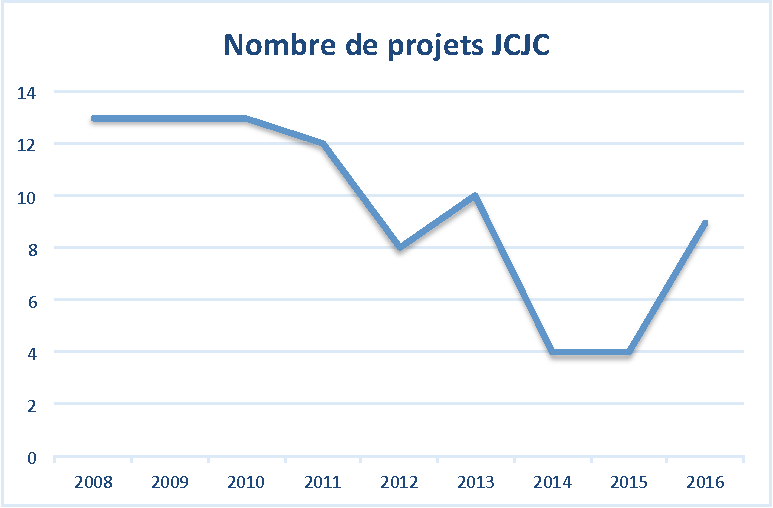
\includegraphics{Images/PastedGraphic-2.pdf}
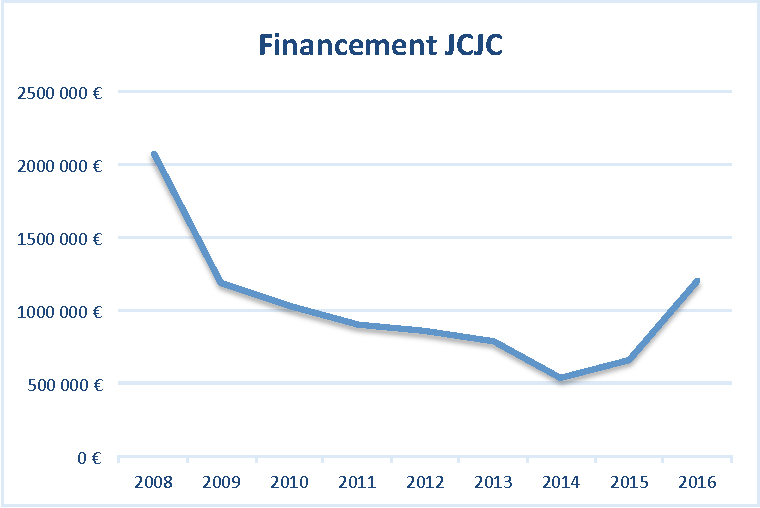
\includegraphics{Images/PastedGraphic-1.pdf}
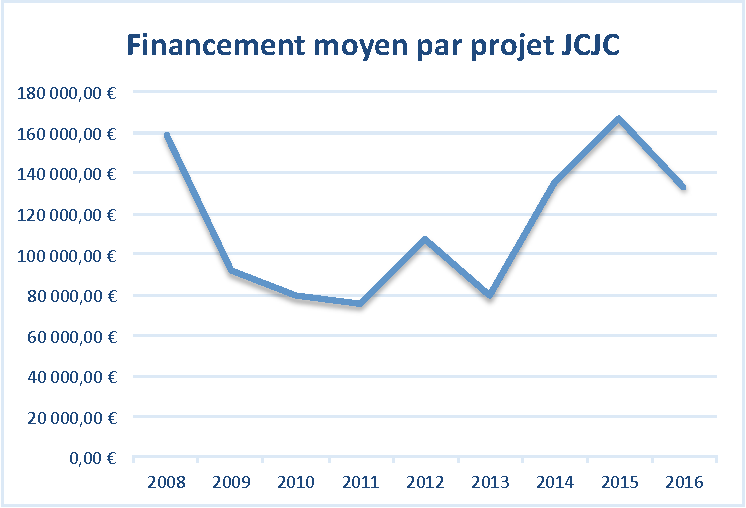
\includegraphics{Images/PastedGraphic-3.pdf}}
\caption{\'Evolution du financement JCJC}
\label{fig:anr}
\end{figure}

Concluons en remarquant que sur les deux ann\'ees 2017 et 2018 le taux de succès global en nombre de projets a \'et\'e de 21,6\% pour le CES 40 mais de 17,6 \% en montant d'aide.

%%%%%%%%%%%%%%%%%%%%%%%%%%%%%%%%%%%%%%%%%%%%%%%%
%%%%%%%%%%%%%%%%%%%%%%%%%%%%%%%%%%%%%%%%%%%%%%%%

\section{Les EX: ``initiatives d'excellence'' \& co.}\label{trucenex}
Une introduction au programme d'\og{}investissement d'avenir\fg{} peut \^etre trouv\'ee sur la page du minist\`ere: \\
{\small \lien{www.enseignementsup-recherche.gouv.fr/pid24578/investissements-d-avenir.html}} \\
ainsi que sur le site de l'ANR : 
\lien{www.agence-nationale-recherche.fr/investissementsdavenir/}. 

Le premier Programme Investissements d'Avenir (PIA1) proposait, en juillet-septembre 2010, 35 milliards d'euros, 
dont 22 milliards d'euros destin\'es \`a l'enseignement sup\'erieur et \`a la recherche.
L'ANR a {\'e}t{\'e} op{\'e}rateur du PIA1 (et est l'op{\'e}rateur du PIA2, voir ci-dessous) 
pour tout ce qui concerne la recherche et l'enseignement sup{\'e}rieur. 
A ce titre, elle a {\'e}t{\'e} charg{\'e}e du suivi administratif et financier des projets, 
il existe d'autres op{\'e}rateurs (CEA, Caisse des D{\'e}pôts par exemple). 
Le financement est totalement distinct du celui des projets du paragraphe pr{\'e}c{\'e}dent.

Les investissements d'avenir se d\'eclinent en plusieurs ``actions'', qui sont des appels d'offres dont les laur\'eat$\cdot$es 
se partagent le budget allou\'e \`a l'action :
\begin{itemize}
\item Laboratoire d'excellence (Labex), appel d'offres pour financer des projets de laboratoires pouvant s'appuyer 
sur des laboratoires ou regroupement de laboratoires existants ; 
le portail des Labex de Math{\'e}matiques (en un sens large) se trouve {\`a}  \lien{labex.math.cnrs.fr}. 
Notons que l'IHP, le CIRM, l'IHES let Cimpa sont dans le labex Carmin ; %qui est l'un des deux labex nationaux en math{\'e}matiques (l'autre, c'est AMIES, cf. \eqref{AMIES}) ;
\item \'Equipement d'excellence (Equipex), appel d'offres pour financer l'achat d'\'equipement de recherche 
de taille interm\'ediaire (entre 1 et 20 millions d'euros) au service d'un projet scientifique et 
essentiel \`a la vie des laboratoires.
\end{itemize}

\`A ces actions, s'ajoutent d'autres actions dont on pourra trouver les descriptifs sur la page du minist\`ere. 
On distingue d'une part les actions de valorisation, dont l'objet est de favoriser
la traduction des d\'ecouvertes scientifiques en applications industrielles et commerciales 
(licences, partenariats industriels, cr\'eation d'entreprises, mobilit\'e des chercheuses et chercheurs publics vers le priv\'e), 
en donnant l'un des labels suivants.
\begin{itemize}
\item Instituts Carnot : laboratoire, groupe de laboratoires ou \'etablissement qui s'engage dans la recherche partenariale 
et qui collabore efficacement avec des entreprises.
\item Instituts de recherche technologique (I.R.T.) : regroupement de laboratoires publics et priv\'es consacr\'e 
\`a un domaine technologique d'avenir. Il rassemble, dans un p\'erim\`etre g\'eographique restreint, des activit\'es de formation, 
de recherche et d'innovation.
\item Institut hospitalo-universitaire (I.H.U.) : p\^ole d'excellence au sein de l'h\^opital et de l'universit\'e 
qui regroupe des services de soins reconnus, des \'equipes de recherche biom\'edicale de r\'eputation mondiale, 
un enseignement universitaire de qualit\'e et une valorisation des d\'ecouvertes.
\item Soci\'et\'es d'acc\'el\'eration du transfert de technologie (S.A.T.T.) : 
ces filiales majoritairement d\'etenues par un ou plusieurs \'etablissements renforceront la diffusion des r\'esultats 
de la recherche vers le monde industriel.
\end{itemize}
D'autre part, on distingue deux ``op\'erations''.
\begin{itemize}
\item Op\'eration campus : c'est un plan de r\'enovation de l'immobilier universitaire de grande ampleur.
\item Op\'eration du plateau de Saclay : cette op\'eration vise \`a cr\'eer sur le plateau de Saclay 
un des tous premiers centres scientifiques et technologiques mondiaux.
\end{itemize}

La coordination, la s\'election et le suivi de ces projets sont confi\'es \`a
un commissariat g\'en\'eral \`a l'investissement. Louis Schweitzer a succ\'ed\'e \`a Louis Gallois en 2014.

Le second Programme Investissements d'Avenir (PIA2) a \'et\'e lanc\'e en 2014 avec un budget de 12 milliards
d'euros. Il a pour objectif de \og{}renforcer [la] comp\'etitivit\'e, au service de l'emploi,
et le d\'eveloppement durable de [l']\'economie.\fg{}
Il comprend entre autres la poursuite de l'action IDEX et son extension I-SITE
dans le but de renforcer la structuration de la recherche et de l'enseignement sup\'erieur fran\c cais.

Il existe un PIA3, qui est annonc{\'e} comme mettant l'accent sur la p{\'e}dagogique.
Voici des liens pour plus d'informations : \\
\lien{www.enseignementsup-recherche.gouv.fr/cid104012/index.html} \\
\lien{www.letudiant.fr/educpros/actualite/pia-3.html} 

Tous ces projets ont une dur{\'e}e de vie limit{\'e}e (fin 2019 pour les LabEx et EquipEx par exemple). 
Leur survie apr{\`e}s cette date d{\'e}pend entre autres de leur appartenance ou non {\`a} une IdEx, voir paragraphe suivant.

\subsection{IDEX/I-SITE}

Les Initiative d'excellence Idex I-SITE, pour Initiatives Science – Innovation –Territoires – Economie, sont des appels d'offres encourageant le montage de projets scientifique r\'eunissant, selon une logique de territoire, des \'etablissements d'enseignement sup\'erieur et de recherche. Toutes les informations
peuvent \^etre trouv\'ees \`a l'adresse suivante :
\href{http://www.agence-nationale-recherche.fr/investissements-d-avenir/appels-a-projets/2014/initiatives-dexcellence-idex-initiatives-science-innovation-territoires-economie-i-site/?L=jae}{%
\texttt{Site de l'ANR > Investissements d'avenir > Appels \`a projets > Idex/I-SITE}}

Il s'agit d’une action lanc{\'e}e dans le cadre du premier et second programme d'Investissements d’avenir. 
Pour r{\'e}sumer, un I-SITE c'est:
\begin{itemize}
 \item Un projet scientifique sur des th{\'e}matiques d{\'e}j{\`a} en pr{\'e}sence et reconnues.
 \item Le d{\'e}veloppement de coop{\'e}rations avec le monde socio{\'e}conomique.
 \item Une structuration institutionnelle et de la gouvernance faisant {\'e}merger une \textit{universit{\'e} cible}.
\end{itemize}

L{\`a} o{\`u} il y des Idex ou Isite, il y a des appels d'offre auxquels les math\'ematicien$\cdot$nes peuvent candidater.
Une liste peut {\^e}tre trouv{\'e}e sur \href{https://fr.wikipedia.org/wiki/Initiative_d'excellence}{Wikipedia}!

%L'appel \`a projets ``Initiatives d'excellence", dot\'e de 6,35 milliards d'euros (initialement, 7,7 milliards d'euros issus du grand emprunt avaient \'et\'e annonc\'es), doit permettre de faire \'emerger en France 5 \`a 10 p\^oles pluridisciplinaires d'excellence d'enseignement sup\'erieur et de recherche de rang mondial. L'objectif des initiatives d'excellence est de r\'eunir, autour de projets scientifiques, mais aussi en incluant une logique de territoires, des \'etablissements d'enseignement sup\'erieur et de recherche, afin de leur assurer davantage de visibilit\'e et d'attractivit\'e \`a l'\'echelle internationale. \\
%
%
%Il y a pour l'instant eu deux appels \`a projets, en janvier 2011 (\'edition 2010) puis en septembre 2011 (\'edition 2012).
%Sur les 17 candidatures de janvier 2011, 3 projets ont \'et\'e s\'electionn\'es : Bordeaux, Strasbourg et Paris Sciences Lettres. Pour la seconde vague, 5 projets sur 11 candidatures sont retenus : Sorbonne universit\'es, Sorbonne Paris Cit\'e, Saclay, Aix-Marseille et Toulouse. La s\'election des projets faisait intervenir une phase de pr\'e-s\'election. Les candidatures ont \'et\'e \'evalu\'ees par un jury international et \'etaient jug\'ees sur les points suivants :
%\begin{itemize}
%\item l'excellence en mati\`ere de recherche,
%\item l'excellence en mati\`ere de formation et la capacit\'e \`a innover,
%\item l'intensit\'e des partenariats avec l'environnement socio-\'economique et au niveau international,
%\item la capacit\'e de la gouvernance \`a mettre en {\oe}uvre efficacement  la strat\'egie du projet : objectifs et trajectoire, politique des ressources humaines, allocation des moyens.
%\end{itemize}
%Lors de la phase probatoire de quatre ans, une part des revenus des 6,35 milliards d'euros sera vers\'ee \`a chacun des 8 campus s\'electionn\'es pour financer les premi\`eres d\'epenses de mise en {\oe}uvre de son projet. Apr\`es la p\'eriode probatoire de 4 ans, et en fonction des objectifs atteints, chaque campus labellis\'e recevra une dotation en capital dont les revenus assureront leur financement dans la dur\'ee. La dur\'ee d'un Idex est 10 ans. Cette dotation, qui pourra aller jusqu'\`a 1 milliard d"euros, viendra compl\'eter les fonds priv\'es lev\'es.\\
%
%La d\'emarche des IDEX a \'et\'e critiqu\'ee. Il a \'et\'e reproch\'e aux IDEX d'avoir \'et\'e \'elabor\'es en dehors des instances r\'eguli\`eres des universit\'es et d'\^etre bas\'es sur une concurrence exacerb\'ee entre \'etablissements et d'\^etre bas\'e sur du financement par projet, jug\'e destructeur pour l'universit\'e. Voir par exemple\\
%\lien{www.sauvonsluniversite.com/spip.php?article5440}.
%
%\subsection{Labex}
%
%
%L'objectif de cet appel d'offre est de faire \'emerger des laboratoires d'excellence dans tous les territoires et toutes les disciplines afin de favoriser l'\'emergence de projets scientifiques de laboratoires ou groupes de laboratoires visibles \`a l'\'echelle internationale. Un fonds d'1 milliard d'euros est cr\'e\'e dont les revenus permettront d'assurer le financement des laur\'eats. Les financements sont accord\'es et attribu\'es pour 10 ans aux laur\'eats et permettent aux laboratoires de renforcer leur excellence scientifique et leur comp\'etitivit\'e au niveau international, ou encore de mettre en place des projets de formation innovants de niveau master ou doctorat. Ces financements ont vocation \`a \^etre compl\'et\'es par des cofinancements de la part des collectivit\'es locales et des partenaires priv\'es. Le financement est pr\'evu sur une p\'eriode de 10 ans avec une \'evaluation interm\'ediaire.\\
%
%
%Lors de la premi\`ere vague d'appels \`a projets, 100 laur\'eats ont \'et\'e d\'esign\'es. \`A la seconde vague, ce sont 71 laur\'eats qui ont \'et\'e choisis.
%L'ensemble des domaines de recherche est repr\'esent\'e parmi les projets retenus.



%\subsection{Equipex}
%
%Cet appel \`a projets, vise \`a doter la France d'\'equipements scientifiques de taille interm\'ediaire (c'est-\`a-dire entre 1 et 20 millions d'euros) de qualit\'e, qui pourront b\'en\'eficier \`a l'ensemble des domaines de recherche. L'utilisation d'\'equipements scientifiques r\'eguli\`erement renouvel\'es, conformes aux standards internationaux, est en effet devenue dans la plupart des disciplines scientifiques une condition imp\'erative de comp\'etitivit\'e au niveau international.\\
%
%
%
%Un fonds de 1 milliard d'euros est cr\'e\'e. Les \'etablissements recevront de l'ordre de 400 millions d'euros pour l'achat de mat\'eriel. Le capital restant produira des int\'er\^ets pour financer le fonctionnement des \'equipements, puis pour relancer de nouveaux appels \`a projets.\\
%
%52 projets ont \'et\'e retenus lors de la premi\`ere vague, et 36 lors de la seconde vague.


\subsection{AMIES }
\index{AMIES} \label{AMIES}
\lien{www.agence-maths-entreprises.fr/}

\noindent AMIES  \og{}Agence pour les Math\'ematiques en Interaction avec l'Entreprise
et la Soci\'et\'e\fg{} a \'et\'e labellis\'e comme Laboratoire d'Excellence au
printemps 2011 dans le cadre du programme investissement d'avenir. Une Unit\'e Mixte de
Service CNRS-UJF (UMS 3458) a \'et\'e cr\'e\'ee le 1er Juin 2011 pour agir
comme support \`a ce LabEx.  AMIES est dirig\'e par \verifier{V\'eronique Maume-Deschamps};  
les deux tutelles de l'UMS sont le CNRS et l'Universit{\'e} Grenoble Alpes (UGA), Inria est partenaire.

AMIES a deux objectifs principaux:
\begin{itemize}
\item  proposer et soutenir des programmes, en formation et recherche,
  visant \`a une meilleure interaction des math\'ematicien$\cdot$nes avec les  entreprises, 
\item offrir aux entreprises, aux chercheur$\cdot$ses et aux \'etudiant$\cdot$es
  une visibilit\'e des opportunit\'es qui existent dans ce domaine. 
\end{itemize}

AMIES est un r\'eseau national en direction des entreprises, et qui concerne toutes les
math\'ematiques et tous les laboratoires.  
L'agence  s'appuie sur un r\'eseau  de facilitateur$\cdot$trices qui sont  les relais de l'agence dans les r\'egions et les universit\'es.
Elles et ils facilitent la mise en relation des entreprises -- et notamment les PME -- et des laboratoires.
Il y a \'egalement, dans tous les laboratoires, des correspondant$\cdot$es maths-entreprises dont la liste est
accessible sur le site web d'AMIES.

Pour les chercheur$\cdot$ses ou enseignant$\cdot$es-chercheur$\cdot$ses en math\'ematiques dans un laboratoire ou un organisme public de recherche,
int\'eress\'e$\cdot$es par des collaborations avec des entreprises,  AMIES offre plusieurs possibilit\'es : 
\begin{itemize}
\item  afficher votre expertise ou vos collaborations
  actuelles dans notre catalogue national,
\item   faire tamponner vos publications en lien avec
  l'interface Maths-Entreprises dans la nouvelle collection HAL
  \og{}Math\'ematiques et Entreprises\fg{}.
\end{itemize}

Les programmes AMIES peuvent aussi vous apporter un soutien :
\begin{itemize}
\item pour amorcer ou renforcer une collaboration avec une
  entreprise avec le programme PEPS (Projet Exploratoire Premier Soutien). Les dossiers d\'epos\'es sont \'etudi\'es
  au fil de l'eau;
\item   pour organiser un atelier ou une conf\'erence visant la
  mise en contact d'entreprises et de chercheur$\cdot$ses ou des \'etudiant$\cdot$es.
\end{itemize}

AMIES finance \'egalement  les Semaines d'\'Etude Maths-Entreprises (SEME) qui sont
organis\'ees par les laboratoires volontaires. 
Le principe des SEME est de faire se rencontrer des industriels et des chercheur$\cdot$ses acad{\'e}miques 
autour de sujets exploratoires. Des industriel$\cdot$les viennent pr{\'e}senter des probl{\`e}mes ouverts, 
dont la formulation m{\^e}me n'est pas toujours aboutie, 
sur lesquels planchent de petits groupes de doctorant$\cdot$es et post-doctorant$\cdot$es, 
{\'e}ventuellement aid{\'e}$\cdot$es par des chercheur$\cdot$ses seniors, pour proposer des embryons de solutions ou des pistes possibles.
La liste des {\'e}ditions pass{\'e}es et {\`a} venir sont sur le site web d'AMIES.
N'h\'esitez pas \`a en parler aux doctorant$\cdot$es ou docteur$\cdot$es r\'ecent$\cdot$es de votre laboratoire et,
pourquoi pas, envisager de participer \`a l'organisation d'une SEME dans votre laboratoire. 

AMIES est {\'e}galement associ{\'e}e {\`a} de nombreux {\'e}v{\'e}nements, congr{\`e}s, formations... 
comme par exemple le CEMRACS, le Forum Emploi Maths (FEM), les RMI (Rencontres Math{\'e}matiques Industries) 
avec la SMAI ou les RII (Rencontre Inria Industrie).

Pour toutes questions,  n'h\'esitez pas  \`a consulter le site web AMIES 
et \`a  contacter le correspondant maths-entreprises de votre laboratoire (\lien{www.agence-maths-entreprises.fr/a/?q=fr/node/267/}).

%%%%%%%%%%%%%%%%%%%%%%%%%%%%%%%%%%%%%%%%%%%%%%%%
%%%%%%%%%%%%%%%%%%%%%%%%%%%%%%%%%%%%%%%%%%%%%%%%


%%%%%%%%%%%%%%%%%%%%%%%%%%%%%%%%%%%%%%%%%%%%%%%%
%%%%%%%%%%%%%%%%%%%%%%%%%%%%%%%%%%%%%%%%%%%%%%%%

\section{Programmes europ\'eens}

\subsection{ERC Starting Grant}
\index{ERC Starting Grant}

Partant du constat que l'offre europ\'eenne d'opportunit\'es de carri\`ere pour les jeunes chercheuses et jeunes chercheurs est
 beaucoup trop faible, le \textit{European Research Council} (ERC) a mis en place 
 des \textit{Starting Grants}
\`a destination des jeunes chercheurs et chercheuses issu$\cdot$es d'instituts europ\'eens. Ce programme a pour but de soutenir
 les projets des jeunes chercheur$\cdot$ses ou enseignant$\cdot$es-chercheur$\cdot$es de fa\c con \`a favoriser leur prise de
responsabilit\'e, leur permettre de d\'evelopper de fa\c con autonome une th\'ematique propre, 
et leur donner la possibilit\'e d'exprimer rapidement leur capacit\'e d'innovation. \\

\textbf{Les \textit{Starting Grants} en bref}~:
\begin{itemize}
\item Candidatures~: la proposition doit \^etre ambitieuse et novatrice.
\item Porteur$\cdot$se de projet~: il n'y a pas de crit\`ere de nationalit\'e. La th\`ese doit avoir \'et\'e soutenue il y a plus de deux ans, et moins de sept ans (des d\'erogations sont possibles sur justification, par exemple en cas de grossesse au cours de la p\'eriode). La porteuse ou le porteur ne doit pas n{\'e}cessairement occuper un \textit{poste de permanent}.
\item Institution du ou de la porteur$\cdot$se de projet~: n'importe quel organisme (public ou priv\'e) reconnu comme tel par l'Union Europ\'eenne.
\item Financement~: jusqu'\`a 1.5\,M\euro{} (parfois m\^eme 2) sur la totalit\'e du projet.
\item Dur\'ee du projet~: jusqu'\`a cinq ans.
\item Appel d'offre~: annuel, publi\'e en \'et\'e avec une date butoir \`a l'automne.
\item \'Evaluation~: par les pairs, 25 scientifiques ind\'ependant$\cdot$es, et couvrant l'ensemble des domaines de recherche. Cette {\'e}valuation contient une premi{\`e}re phase sur dossier, puis une seconde {\`a} l'oral.
\end{itemize}
\index{ERC Starting Grant}
Pour en savoir plus, t\'el\'echarger le guide du$\cdot$de la candidat$\cdot$e ou celui du$\cdot$de la rapporteur$\cdot$trice (\'egalement utile pour les candidates et candidats !), aller \`a l'adresse 
\lien{erc.europa.eu/starting-grants/}.


\subsection{Horizon Europe}
\index{Programme cadre europ\'een}

\verifier{Horizon Europe}, le programme de recherche et d'innovation de l'Union europ\'eenne 
recentre les financements sur trois priorit\'es : 
l'excellence scientifique, la primaut\'e industrielle, les d\'efis soci\'etaux. 
\verifier{Il est dot\'e de 95,5 milliards d'euros, pour la p\'eriode de 2021-2027}. \\
\lien{https://www.horizon-europe.gouv.fr/}


\section{Les programmes Campus France}
\index{Campus France}
\index{Partenariat Hubert-Curien (PHC)}

Cr\'e\'ee par la loi du 27 juillet 2010, L'Agence Campus France est un nouvel \'etablissement public (EPIC) charg\'e de la promotion de l'enseignement sup\'erieur, de l'accueil et de la gestion de la mobilit\'e internationale des \'etudiants, des chercheurs, des experts et des invit\'es. Un d\'ecret du 30 d\'ecembre 2011 pr\'ecise l'organisation et les modalit\'es d'action de l'Agence. R\'esultant de la fusion du GIP Campus France et de l'association \'Egide, l'\'etablissement est plac\'e sous la tutelle des minist\`eres des Affaires \'etrang\`eres et europ\'eennes et de l'Enseignement sup\'erieur et de la Recherche. \\
\lien{www.campusfrance.org/fr/page/lagence-campus-france}. \\

\textbf{Les partenariats Hubert-Curien (PHC)} :
\label{PHC}
Un partenariat est un projet de recherche, {\'e}tabli conjointement par deux {\'e}quipes de recherche, l'une fran\c{c}aise, l'autre {\'e}trang{\`e}re, qui b{\'e}n{\'e}ficient apr{\`e}s {\'e}valuation du soutien financier des deux instances partenaires.
L'objectif des PHC est de d{\'e}velopper les {\'e}changes scientifiques et technologiques entre les laboratoires de recherche des deux communaut{\'e}s scientifiques, en favorisant les nouvelles coop{\'e}rations. 
Les financements sont accord\'es sur une base annuelle. Ils doivent donc imp\'erativement \^etre consomm\'es entre le 1er janvier et le 31 d\'ecembre de l'ann\'ee concern\'ee et ne peuvent \^etre report\'es sur l'exercice suivant.
Une attention particuli{\`e}re est par ailleurs apport{\'e}e aux projets pr{\'e}sent{\'e}s par des {\'e}quipes nouvelles et aux sujets r{\'e}ellement novateurs ainsi qu'aux projets d{\'e}pos{\'e}s dans le cadre de plusieurs PHC. En outre, les jeunes scientifiques sont fortement encourag{\'e}$\cdot$es {\`a} s'impliquer comme chefs de projet.
\lien{http://www.campusfrance.org/fr/phc}

\section{Les autres programmes nationaux et internationaux}
Il existe plusieurs types de sources de financement pour des projets
scientifiques de collaborations internationales. Nous en pr\'esentons
ici quelques-uns.

\subsection{Les projets PRC du CNRS}

Le CNRS, dans le cadre des accords de coop{\'e}ration qu'il a sign{\'e}s avec certaines agences de financement ou organismes de recherche {\'e}trangers, 
finance des Projets de Recherche Conjoints (PRC), permettant {\`a} deux {\'e}quipes de chercheur$\cdot$ses de travailler ensemble. 
La participation de jeunes chercheur$\cdot$ses est fortement encourag{\'e}e.
Le PRC est {\'e}valu{\'e} et s{\'e}lectionn{\'e} conjointement par le CNRS et l’organisme partenaire. \\
\lien{www.cnrs.fr/derci/spip.php?article50}
\index{Projets de Recherche Conjoints (PRC)}

\subsection{Les projets PEPS du CNRS}

L'Insmi (CNRS) pilote aussi des appels d'offre permettant aux chercheuses et chercheurs de disposer de financement pour une p\'eriode donn\'ee (un \`a deux ans) sur projet scientifique. 
Ces projets appel\'es {\it Projets exploratoires premiers soutiens} (Peps) sont l\'egers \`a monter. 
Ils peuvent \^etre totalement financ\'e par l'Insmi comme le projet {\it Peps-Jeunes chercheur$\cdot$ses}, ou bien \^etre mont\'es avec 
d'autres instituts ainsi que la Mission interdisciplinarit\'e du CNRS (\lien{http://www.cnrs.fr/mi/}). 
Via la Direction de l'innovation et des relations avec les entreprises (\lien{http://www.cnrs.fr/dire/}), 


\subsection{Les projets ECOS}
Les programmes d'\'evaluation-orientation de la coop\'eration
scientifique (ECOS) concernent sp\'eci\-fi\-que\-ment les
partenariats avec l'Am\'erique du Sud. Ils financent les \'echanges
entre les chercheuses ou chercheurs sous la forme de missions de courte dur\'ee, de
stages de perfectionnement et de bourses doctorales. \\
\lien{www.univ-paris13.fr/cofecub-ecos/}
\index{Evaluation-orientation de la coop\'eration scientifique (ECOS)}

\subsection{Les PICS} \label{PICS}
Les programmes internationaux de coop\'eration scientifique (PICS)
sont financ\'es par le CNRS.
Ce sont des projets de plus grande taille que les PHC, regroupant un
ou plusieurs partenaires. Ils sont mis en place pour trois ans (avec
possibilit\'e d'extension). Ils permettent principalement le
financement d'accueils et de missions, d'organisation de
s\'eminaires et de r\'eunions de travail, mais aussi d'une partie du
surco\^ut de fonctionnement d\^u \`a la gestion du PICS, voire
exceptionnellement d'\'equipements l\'egers. \\
\lien{www.cnrs.fr/derci/spip.php?article51}
\index{Programmes internationaux de coop\'eration scientifique (PICS)}

\subsection{Les \'equipes associ\'ees Inria}
\index{Inria}
Le programme Inria \textit{\'Equipes associ\'ees} a pour but de d\'evelopper les collaborations internationales
d'Inria avec des \'equipes de recherche \'etrang\`eres.
Ce financement de  longue dur\'ee permet d'am\'eliorer la mobilit\'e de chercheur$\cdot$ses,
d'\'etudiant$\cdot$es et de post-doctorant$\cdot$es, d'organiser conjointement  des conf\'erences...
Ce programme est d'une grande souplesse dans la mani\`ere d'utiliser les cr\'edits de financement et
 encourage particuli\`erement la mobilit\'e des \'etudiant$\cdot$es et jeunes chercheur$\cdot$ses. Le lien suivant donne plus d'informations: \\ 
\lien{www.inria.fr/recherches/mobilite-internationale/equipes-associees/programme}

\section{Les contrats industriels}
Les contrats de recherche avec des partenaires industriels prennent
une place importante dans les sources de financement de la recherche en
math\'ematiques appliqu\'ees. La gestion d'un contrat d\'epend
consid\'erablement de l'\'etablissement de recherche signataire du
contrat, il est donc difficile d'\'enoncer des r\`egles
g\'en\'erales sur la question. Il peut cependant \^etre utile d'indiquer
qu'il est parfois possible pour les intervenant$\cdot$es
enseignant$\cdot$es-chercheur$\cdot$ses du contrat d'acheter, avec l'argent du
contrat, \`a leur UFR ou \`a leur d\'epartement d'enseignement une
partie de leurs heures d'enseignement statutaires.
\index{Contrats industriels}


%%%%%%%%%%%%%%%%%%%%%%%%%%%%%%%%%%%%%%%%%%%%%%%%%%
%%%%%%%%%%%%%%%%%%%%%%%%%%%%%%%%%%%%%%%%%%%%%%%%%%
\part{La communaut\'e math\'ematique}

%%%%%%%%%%%%%%%%%%%%%%%%%%%%%%%%%%%%%%%%%%%%%%%%%%
%%%%%%%%%%%%%%%%%%%%%%%%%%%%%%%%%%%%%%%%%%%%%%%%%%

\chapter{Les soci\'et\'es savantes}

Nous remercions les soci\'et\'es savantes qui ont aid\'e \`a la r\'edaction des textes ci-dessous et participe activement \`a l'organisation de cette journ\'ee.

%%%%%%%%%%%%%%%%%%%%%%%%%%%%%%%%%%%%%%
\section{La SMAI}

\emph{Pr\'esident\mp e actuel\mp le : \verifier{Olivier Goubet}} \hfill Site web : \url{http://smai.emath.fr}%, Facebook-Twitter : @smai-media
\smallskip

La SMAI (Soci\'et\'e de Math\'ematiques Appliqu\'ees et
Industrielles), une soci\'et\'e savante en math\'ematiques
appliqu\'ees... pour quoi faire ?

Quand on parle de \og soci\'et\'e savante\fg{}, en particulier chez
les jeunes scientifiques, il y a souvent deux types de
r\'eactions~:
\begin{itemize}%[leftmargin=2em,itemsep=0.4ex]
    \item \og Ouh l\`a, c'est du s\'erieux ...
pour en faire partie il doit falloir \^etre quelqu'un de tr\`es
tr\`es fort et \c{c}a doit parler de choses dr\^olement
compliqu\'ees ... \fg{},
\item \og C'est un peu vieillot et rempli de personnes qui
n'ont que \c ca \`a faire ...\fg{}
sans d'ailleurs savoir ce que \og \c ca\fg{}
repr\'esente.
\end{itemize}

Rien n'est plus faux. Les soci\'et\'es savantes en math\'ematiques
s'attachent \`a \^etre aux c\^ot\'es des math\'ematiciens dans
toutes leurs activit\'es professionnelles
(dans le monde acad\'emique ou industriel),
en particulier l\`a o\`u les structures font d\'efaut.

Malgr\'e toutes les actions que ces soci\'et\'es organisent
directement ou soutiennent, il y a encore beaucoup \`a
faire. Et c'est justement des jeunes que nos soci\'et\'es savantes ont
besoin... Parce qu'il s'agit bien de leur vie scientifique et
de leur avenir professionnel.

Le domaine de la recherche en math\'ematiques est fragile parce que difficile \`a
cerner et \`a expliquer. La SMAI est n\'ee du constat
que la sp\'ecificit\'e des math\'ematiques appliqu\'ees et industrielles devait \^etre
identifi\'ee et d\'efendue si la discipline voulait prosp\'erer. Les
applications des math\'ematiques s'entendent au sens le plus large,
en lien avec les autres sciences et avec les probl\'ematiques
soulev\'ees par des entreprises et qui n\'ecessitent des comp\'etences de math\'ematicien\mp ne\mp s.

L'un des premiers r\^oles de la SMAI est de les aider \`a nouer des contacts dans la communaut\'e
et en dehors, en France et \`a l'\'etranger \`a travers notamment
l'organisation
\begin{itemize}%[noitemsep,topsep=-\parskip,leftmargin=2em]
    \item des journ\'ees th\'ematiques Maths-Industrie ;
    \item des congr\`es (Congr\`es SMAI, journ\'ees des groupes th\'ematiques, CANUM, ...) ;
    \item du CEMRACS, une \'ecole d'\'et\'e sur 6 semaines au CIRM sur le calcul scientifique
	au sens large ;
    \item l'\'ecole franco-espagnole Jacques-Louis Lions sur la simulation num\'erique en
	physique et ing\'enierie ;
    \item des colloques co-organis\'es \`a l'\'etranger (Mexique, ...) ;
    \item ...
\end{itemize}
mais aussi \`a travers des actions communes avec des soci\'et\'es
s\oe urs fran\c caises (SFdS, SMF), \'etrang\`eres (en Italie, Espagne, ...)
des participations aux conseils d'instances et associations internationales (ICIAM,
EMS, ECCOMAS, ...), le parrainage de colloques, ...

La communication entre les membres de la SMAI se fait par le bulletin de
liaison \emph{Matapli} (3 num\'eros par an) et par la lettre \'electronique
\texttt{smai-info}, dont l'abonnement est ouvert \`a tous. De nombreuses
informations et actualit\'es se trouvent sur le site de la SMAI qui fait partie
du domaine \texttt{emath} regroupant divers sites de la communaut\'e
math\'ematique dont certains sont soutenus ou initi\'es par la SMAI~:
Agenda des Conf\'erences en Math\'ematiques, Op\'eration Postes, Carte des Masters, ...

Concernant l'emploi scientifique (postes acad\'emiques, dans les organismes de recherche ou dans les entreprises), la SMAI soutient des activit\'es
telles que
\begin{itemize}%[noitemsep,topsep=-\parskip,leftmargin=2em]
    \item le Forum Emploi Math\'ematiques, qu'elle co-organise ;
    \item l'Op\'eration Postes ;
\end{itemize}
et
\begin{itemize}%[noitemsep,topsep=-\parskip,leftmargin=2em,after={\\}]
    \item a publi\'e un \og livre blanc sur la valorisation dans l'industrie du dipl\^ome de docteur en math\'ematiques appliqu\'ees\fg{} ;
    \item joue le r\^ole d'expertise aupr\`es d'institutions
	nationales (minist\`ere, CNRS, ...) et europ\'eennes
	pour les questions li\'ees aux math\'ematiques appliqu\'e.
\end{itemize}

Pour assurer la diffusion des travaux des math\'ematiciens
appliqu\'ees, la SMAI \'edite les collections d'ouvrages
\emph{Math\'ematiques et applications} (Springer), \emph{Math\'ematiques appliqu\'ees
pour le Master/SMAI} (Dunod) ainsi que les revues de la collection
ESAIM (chez EDP Sciences)~: 
	\begin{itemize}
		\item M2AN (mod\'elisation math\'ematique et analyse num\'erique)
		\item COCV (contr\^ole optimal et calcul des variations)
		\item P\&S (probabilit\'es \& statistiques)
		\item ProcS (proceedings and surveys)
	\end{itemize}
ainsi que RAIRO-RO (avec la ROADEF) et Maths in Action. De plus, la SMAI a lanc\'e le \textbf{SMAI Journal of Computational Mathematics}
(SMAI-JCM), journal \'electronique gratuit.

De m\^eme, elle participe \`a des prix scientifiques,
dont plusieurs sont d\'ecern\'es par l'Acad\'emie des Sciences,
un autre au niveau international, ainsi que des prix
de th\`ese pour promouvoir les travaux de jeunes docteurs.

La SMAI ne se limite pas \`a cr\'eer
des liens entre les communaut\'es. Elle participe aussi largement aux questions
d'enseignement des math\'ematiques en lien avec les autres disciplines et les r\'eformes, du coll\`ege \`a l'universit\'e
et aux grandes \'ecoles,
apportant l\`a aussi son expertise en
participant \`a divers conseils et comit\'es, et en prenant
des positions publiques.

La SMAI est aussi fortement investie dans des actions
de promotion et d'explication au niveau du public,
souvent de fa\c con conjointe avec d'autres soci\'et\'es
(SMF, SFdS, ...) ou associations (Animath,~...).  Citons
par exemple, la publication de la brochure \og L'explosion
des math\'ematiques\fg{}, traduite en plusieurs langues
, la brochure \og Zoom sur les m\'etiers
des math\'ematiques\fg{} en partenariat avec l'Onisep (qui va \^etre r\'e-actualis\'ee),
des r\'eunions, d\'ebats et conf\'erences grand public, des actions
dans le cadre de l'ann\'ee internationale
\og Math\'ematiques pour la Plan\`ete Terre 2013\fg{},
l'organisation, conjointement avec INRIA, du
\og forum des laur\'eats des prix en informatique
et math\'ematiques appliqu\'ees\fg{}, ...

Parmi les actions grand public r\'ecentes de la SMAI, on peut citer:
\begin{itemize}
 \item l'organisation d'une journ\'ee Shannon (4 novembre 2016) \`a l'occasion du centi\`eme anniversaire de sa naissance.
 Cette rencontre grand public s'est d\'eroul\'ee au CIRM en collaboration avec le groupe SMAI-SIGMA.
\lien{www.fr-cirm-math.fr/hommage-claude-shannon.html}
Les conf\'erences on \'et\'e  film\'ees et sont disponibles sur la chaine YouTube du CIRM.
\item Semaine des math\'ematiques 2019. Le th\`eme choisi cette ann\'ee pour la semaine des math\'ematiques \'etait \textit{Jouons ensemble aux Math\'ematiques}.
\item Cycle SMAI/Mus\'ee des Arts et M\'etiers, dont les derniers expos\'es furent donn\'es par Ir\`ene Waldspurger et Patrick Joly. 
\item Salon de l'ONISEP o\`u la SMAI participe au stand tenu par les soci\'et\'es savantes.
\end{itemize}

A l'int\'erieur de la SMAI, les actions sont coordonn\'ees et d\'ecid\'ees par un
Conseil d'Administration de 24 membres, renouvel\'e par tiers tous
les ans, et par un bureau.

Certaines des activit\'es plus sp\'ecifiques
\`a des domaines de recherche sont organis\'ees
par les groupes th\'ematiques~:
\begin{itemize}%[noitemsep,topsep=-\parskip,leftmargin=2em,label={$\star$}]
    \item SMAI-GAMNI (Groupe th\'ematique pour l'Avancement des M\'ethodes Num\'eriques de l'Ing\'enieur) ;
    \item SMAI-MABIOME (Math\'ematiques Biologie M\'edecine) ;
    \item SMAI-MAIRCI (Math\'ematiques Appliqu\'ees, Informatique, R\'eseaux, Calcul, Industrie) ;
    \item SMAI-MAS (Mod\'elisation Al\'eatoire et Statistique) ;
    \item SMAI-MODE  (Math\'ematiques de l'Optimisation et de la D\'ecision) ;
    \item SMAI-SIGMA (Signal - Image - G\'eom\'etrie - Mod\'elisation - Approximation).
\end{itemize}
Il est possible d'appartenir \`a plusieurs de ces groupes ... ou \`a aucun.


La SMAI est une soci\'et\'e vivante, forte de 1\,200 adh\'erents
et repr\'esentative des math\'ematiques appliqu\'ees, mais
qui ne vit que par des membres actifs qui adh\`erent pour
\begin{itemize}%[noitemsep,topsep=-\parskip,leftmargin=2em,label={\ding{51}}]
    \item assurer sa repr\'esentativit\'e,
    \item \^etre force de proposition,
    \item am\'eliorer ses prises de d\'ecision,
    \item et soutenir ses actions.
\end{itemize}
Il existe de nombreuses fa\c cons de s'impliquer dans la SMAI
(participer au Conseil d'Administration, \^etre correspondant local,
proposer ou soutenir des actions, ...).

L'adh\'esion est \textbf{gratuite} pour les doctorants inscrits en th\`ese en France, 
ainsi que pour les docteurs ayant soutenu une th\`ese de math\'ematiques depuis moins de deux ans.

Elle est de \EUR{25} pour les moins de 35 ans.

%%%%%%%%%%%%%%%%%%%%%%%%%%%%%%%%%%%%%%%%%%%
\section{La SFdS}
\index{Soci\'et\'e fran\c caise de statistique (SFdS)}

\emph{Pr\'esident\mp e actuel\mp le~: \verifier{Anne Philippe}} \hfill Site web~: \url{https://www.sfds.asso.fr/}
\smallskip

La Soci\'et\'e Fran\c{c}aise de Statistique est une association d\'eclar\'ee au Journal Officiel du 23 ao\^ut 1997, qui a \'et\'e reconnue d'utilit\'e publique par d\'ecret du 3 d\'ecembre 1998. Elle compte \`a ce jour environ 1000 membres et une vingtaine d'adh\'erents personnes morales. Elle a vocation \`a rassembler tous les chercheur\mp ses, enseignant\mp es et utilisateur\mp trices de la statistique, quels que soient la nature de leurs fonctions et l'endroit o\`u ils les exercent : elle constitue ainsi un lieu privil\'egi\'e de rencontres, d'\'echanges et de r\'eflexions. La SFdS est aussi l'interlocuteur naturel des pouvoirs publics pour les diverses questions touchant \`a la science statistique et \`a la science des donn\'ees (enseignement, expertise, \'ethique, etc.). Elle vise \`a promouvoir l'utilisation de la statistique, \`a favoriser ses d\'eveloppements m\'ethodologiques et \`a d\'evelopper les \'echanges entre statisticiens travaillant dans les entreprises, les administrations ou des \'etablissements d'enseignement et de recherche.

Une grande partie des activit\'es de la SFdS est d\'evelopp\'ee au sein de groupes sp\'ecialis\'es dans un th\`eme ou un domaine d'application de la statistique (\verifier{au nombre de 15 en 2023}). Ses objectifs, son histoire et son mode de fonctionnement en groupes donnent ainsi \`a la SFdS, dans le paysage des soci\'et\'es savantes fran\c{c}aises une place particuli\`ere. En effet, elle r\'eunit en son sein aussi bien des universitaires que des praticiens issus de l'entreprise ou des administrations.

La SFdS et ses groupes organisent une cinquantaine de manifestations scientifiques annuelles mais aussi des manifestations grand public comme par exemple les Caf\'es de la Statistique, soir\'ees-d\'ebats favorisant la rencontre entre statisticiens et citoyens.

La soci\'et\'e publie trois revues scientifiques \'electroniques, le Journal de la SFdS, la revue Statistique et Enseignement et la revue Statistique 
et Soci\'et\'e. Par ailleurs, elle co-\'edite la revue Case Studies in Business and Industrial Statistics (CSBIGS).

La SFdS agit ainsi en fonction de deux axes compl\'ementaires. Tout d'abord, elle a vocation \`a promouvoir la recherche dans tous les domaines de la statistique (et de la science des donn\'ees). Outre les nombreuses journ\'ees th\'ematiques ou mini colloques organis\'es par les diff\'erents groupes de l'association sur des th\`emes pointus, elle r\'eunit, tous les ans, quatre \`a cinq cents personnes lors des Journ\'ees de Statistique, qui constituent un rendez-vous incontournable de la statistique francophone. Elles sont aussi un des premiers tremplins pour les doctorant\mp es et jeunes chercheur\mp ses dans la communaut\'e, avec les Rencontres des Jeunes Statisticien\mp nes qui ont lieu une ann\'ee sur deux les ann\'ees impaires.

L'autre axe de son action consiste \`a favoriser la divulgation des techniques r\'ecentes issues de la recherche : elle met ainsi en oeuvre des cours sp\'ecialis\'es sur des sujets \'emergents (Journ\'ees d'Etude en Statistique, Ateliers Statistiques) assurant l'interface entre les chercheur\mp ses et les utilisateurs ainsi que les rendez-vous M\'ethodes et Logiciels.

Au del\`a de toutes les actions d'animation de la communaut\'e statistique, actions qui font la richesse de notre association et qui sont men\'ees en 
grande partie par nos groupes, nous portons \`a tous les niveaux le message selon lequel c'est le statisticien qui est le plus \`a m\^eme de traiter correctement les millions de milliards d’octets de donn\'ees g\'en\'er\'ees chaque minute. Nous accompagnons les adaptations n\'ecessaires \`a ce nouveau paradigme. Nous nous effor\c{c}ons de d\'evelopper les activit\'es de la SFdS en dehors de territoire fran\c{c}ais et travaillons \`a l'\'emergence d'un journal de stature internationale.

Le statistique est au coeur des d\'efis de la soci\'et\'e de demain. D\'ecouvrez nos activit\'es en naviguant sur notre site internet et rejoignez-nous, une premi\`ere adh\'esion SFdS ne co\^ute que 10 euros.



%%%%%%%%%%%%%%%%%%%%%%%%%%%%%%%%%%%%%%%%%%%%
\section{La SMF}
\label{smf}
\index{Soci\'et\'e math\'ematique de France (SMF)}
\index{Centre international de rencontres \\ math\'ematiques (CIRM)}

\emph{Pr\'esident\mp e actuel\mp le : \verifier{Fabien Durand}} \hfill Site web :  \url{https://smf.emath.fr/}
\smallskip

La Soci\'et\'e\ Math\'ematique de France (SMF), cr\'e\'ee en 1872, est l'une des plus anciennes  soci\'et\'es savantes de math\'ematiques au monde. C'est une association loi 1901, reconnue d'utilit\'e publique, qui compte actuellement 1790 membres (essentiellement des membres individuels, mais aussi des membres institutionnels, c'est-\`a-dire des laboratoires de recherche, biblioth\`eques, institutions...). Elle est ouverte \`a tous les
math\'ematicien(ne)s, amateurs ou professionnels. Sa mission initiale, {\sl l'avancement et la propagation des \'etudes de Math\'ematiques pures et appliqu\'ees}, s'est \'elargie et adapt\'ee aux \'evolutions de notre \'epoque. La SMF s'int\'eresse aux math\'ematiques  dans leur diversit\'e et sous tous leurs aspects :  avanc\'ees de la recherche, interactions avec les sciences et techniques, \'edition de livres et revues,  structuration de la vie scientifique, enseignement \`a tous niveaux.

Elle est en relation avec les soci\'et\'es et institutions qui poursuivent les m\^emes buts et interagit avec beaucoup d'entre elles. En particulier beaucoup de ses actions sont communes avec la SFdS et la SMAI, \'{e}galement avec Animath, Femmes et Math\'{e}matiques, et bient\^ot la Fondation Blaise Pascal. Elle  travaille \'egalement avec de nombreuses soci\'et\'es math\'ematiques \'{e}trang\`{e}res et organise des congr\`{e}s bilat\'{e}raux.



Le r\^{o}le de la SMF aujourd'hui est multiple, et parfois pas assez visible. {\bf La SMF est sollicit\'ee sur un grand nombre de sujets, et est \`a l'initiative de beaucoup d'autres} (que je vais d\'evelopper ci-dessous). Pour pouvoir r\'epondre aux nombreuses sollicitations, et d\'evelopper de belles actions, le r\^ole et la participation de la communaut\'e et des adh\'erents est fondamental, et c'est pourquoi {\bf votre soutien nous est important.}
\\Pour y adh\'erer, vous pouvez notamment visiter notre site web. Les adh\'esions sont gratuites pendant 3 ans pour toutes les personnes en th\`ese, et seulement \`a 25 euros par an pour les moins de 35 ans. Cette adh\'esion donne droit aux 4 exemplaires de la Gazette, l’acc\`es \'electronique gratuit au expos\'es Bourbaki, 30 pour cent de r\'eduction sur nos livres. Surtout, {\bf votre adh\'esion est un soutien moral fondamental et une source de motivation pour tous les b\'en\'evoles qui s’impliquent dans la SMF - elle nous donne \'egalement une grande cr\'edibilit\'e lorsque nous d\'efendons les math\'ematiques aupr\`es des institutions, administrations, m\'edias.}


\subsection*{Une source d'informations}

 Un des r\^oles de la SMF est de faire diffuser les informations li\'ees aux math\'ematiques au sein de la communaut\'e fran\c caise. Pour ceci, nous utilisons:
 \begin{itemize}
 \item  \emph{la Gazette des math\'{e}\-maticiens}, que re\c{c}oivent tous les adh\'{e}rent(e)s tous les trois mois. La {\em Gazette} a \'et\'e enti\`erement repens\'ee il y a deux ans pour \^etre plus conviviale.
 \item la lettre \'{e}lectronique mensuelle, 
 \item notre compte Twitter @SocMathFr (tr\`es actif!), avec plus de 3300 abonn\'es\
 \item notre site web. Comme notre syst\`eme informatique dans son ensemble a \'et\'e remis \`a jour pour permettre de mieux r\'epondre aux attentes des adh\'erent\mp es et \^etre conformes avec toutes les nouvelles r\'eglementations. Surtout, il nous fournit une assise technique solide pour les ann\'ees qui viennent. N’h\'esitez pas \`a le parcourir et \`a le consulter, de nombreux articles originaux et nos manifestes y paraissent r\'eguli\`erement.
\end{itemize}

Nous parrainons beaucoup de rencontres, dont les annonces sont diffus\'ees sur nos canaux.

\subsection*{Un lieu de r\'{e}flexion} 
\`{A} titre  d'exemple, la SMF s'engage dans les d\'ebats sur la formation des enseignant\mp es ou l'\'{e}volution des licences et masters aussi bien que de l'enseignement secondaire.

Elle prend position sur les structures de l'enseignement sup\'{e}rieur et la recherche.

Elle r\'{e}fl\'{e}chit aux moyens d'attirer les jeunes vers les sciences et vers les m\'{e}tiers scientifiques.  


\subsection*{Un porte-parole de la communaut\'{e} math\'{e}matique}
Sur toutes les questions mentionn\'ees plus haut, la SMF n'est bien s\^ur pas  seule \`a mener des r\'eflexions, et l'un de nos plus importants  r\^oles est celui d'\^etre organisateur  et facilitateur de d\'ebats, comme lors du dernier congr\`es SMF, ou \`a l'initiative de tribunes dont la vocation est de porter la voix des math\'ematiciennes et math\'ematiciens.

 La SMF a vocation, avec ses partenaires, \`{a} \^{e}tre porte-parole de la communaut\'{e} math\'{e}matique fran\c{c}aise aupr\`{e}s des pouvoirs publics, au niveau fran\c cais et international, mais \'egalement aupr\`es de tous les acteurs de la vie publique: m\'edias, entreprises, recruteurs,...

Ainsi, la SMF participe \`a beaucoup de groupes de r\'eflexions, de comit\'es, de jury, ... qu'il serait trop long de mentionner (mais qui n'est pas secr\`ete !!).

\subsection*{Un organisateur de   conf\'erences pour les math\'ematicien(ne)s} 

\begin{itemize}
 \item
Des sessions {\bf Etats de la recherche}   permettent chaque ann\'ee  de s'initier  et de faire un \og \'etat de l'art\fg{} d'un domaine des math\'{e}matiques en pleine expansion. 
\item
Depuis 2017, la SMF a d\'ecid\'e de financer deux fois par an {\bf une semaine de conf\'erence au CIRM} dont les sp\'ecificit\'es sont d'\^etre orient\'ees vers les jeunes (vous!): organisation de mini-cours, journ\'ee r\'eserv\'ee pour des expos\'es aux th\'esard(e)s, post-docs, et jeunes recrut\'e(e)s, avec un financement sp\'ecifique.
\item
En 2016, le {\bf Premier congr\`es de la SMF, SMF2016,} regroupant l'ensemble de la communaut\'e, a \'et\'e organis\'e \`a Tours. Cela a \'et\'e un moment scientifique remarquable  et l'occasion d'intenses \'echanges, toutes les math\'ematiques \'etant repr\'esent\'ees. Devant ce succ\`es, il a \'et\'e  d\'ecid\'e de l'organiser tous les deux ans, le prochain aura lieu \`a Lille en 2018. Venez nombreux vous tenir au courant des derni\`eres avanc\'ees pr\'esent\'ees par celles et ceux qui les ont produites!

\item
La SMF organise \'egalement des {\bf congr\`es joints} avec des soci\'et\'es \'etrang\`eres. Par exemple, un congr\`es avec l'AMS  est en cours de pr\'eparation pour les ann\'ees qui viennent. 

\item Nous participons \`a beaucoup d'autres \'ev\'enements: cette journ\'ee d'accueil des nouveaux ma\^itres de
conf\'erences et charg\'es de recherche bien s\^ur, la remise de prix de l'Acad\'emie des sciences, et bien d'autres...

\end{itemize}


\subsection*{L'organisation et le soutien d'\'{e}v\`{e}nements destin\'es \`a un plus large public} 

\begin{itemize}
 \item
 La SMF coorganise les deux cycles de conf\'erences
{\bf Un texte, un math\'ematicien}   \`a la Biblioth\`{e}que nationale de France  et {\bf Une question, un chercheur} que vous connaissez s\^urement, et qui sont destin\'es aux lyc\'eens et aux classes pr\'eparatoires.
\item
La SMF lance un nouveau cycle {\bf Math\'ematiques \'etonnantes} durant lequel des conf\'erenciers feront d\'ecouvrir, seuls ou en duo avec leur complice, une interaction inattendue entre diff\'erents domaines math\'ematiques ou entre math\'ematiques et applications. Ces conf\'erences de math\'ematiques seront donn\'ees plusieurs fois par an au niveau licence. Le public vis\'e est celui des \'etudiant\mp es d'universit\'e et \'el\`eves de grandes \'ecoles, des professeur\mp es du second degr\'e et des chercheur\mp ses et ing\'enieur\mp es de tout domaine.

\item
Depuis 2017, la SMF organise un {\bf Concours SMF Junior} destin\'e aux \'etudiants encore \`a l'universit\'e. Le but est de promouvoir aupr\`es de ces jeunes la recherche en math\'ematiques sous une forme originale, celle d'un concours par \'equipe sur 10 jours. Je vous invite fortement \`a y participer en proposant des sujets et en motivant vos \'etudiant(e)s !!

\item
La SMF d\'ecerne tous les 2 ans le {\bf Prix d'Alembert}, qui r\'ecompense des initiatives visant \`a la diffusion des math\'ematiques. En 2016, le prix a \'et\'e remis \`a l'association {\em Pi Day} qui organise un spectacle original et scientifique \`a Marseille et en 2018 le laur\'eat f\^ut Mickael Launay.

\item 
La SMF d\'ecerne \'egalement le nouveau {\bf Prix Jacqueline Ferrand} qui r\'ecompense des initiatives p\'edagogiques remarquables autour des math\'ematiques. Le	premier prix Jacqueline Ferrand a \'et\'e attribu\'e en 2018 \`a l’association Maths en vie qui met l’accent mis sur les premiers cycles de l’apprentissage en math\'ematiques, dont l’importance est fondamentale, et l’utilisation parcimonieuse mais extr\^emement pertinente des outils num\'eriques. 

\item
Comme dit plus haut, nous parrainons un tr\`es grand nombre de rencontres et d'\'ev\'enements (Prix Decerf pour la p\'edagogie, Prix Mandelbrot en association avec l'ambassade de Pologne,...), qui sont trop longs \`a lister, mais que vous pouvez consulter \`a tout moment sur notre site!

\end{itemize}


\subsection*{Une maison d'\'{e}dition}
La SMF est une maison d'\'edition ind\'ependante qui publie de nombreux revues et collections. Parlons chiffre:\begin{itemize}
\item
4 journaux: {\bf Bulletins de la SMF, M\'emoires de la SMF, Revue d'Histoire des Math\'ematiques}, et {\bf Ast\'erisque},
\item
Nous sommes les diffuseurs des {\bf Annales de l'ENS}
\item
4 collections d'ouvrages: {\bf Cours sp\'ecialis\'es,
Documents math\'ematiques, Panoramas et Synth\`eses, S\'eminaires et Congr\`es},

\item
d'autres collections: SMF/AMS Texts and Monographs, S\'erie T, S\'erie Chaire Morlet, Fascicules des journ\'ees annuelles.
\item
 8.000 pages uniques par an

\item
 environ 4.000.000 pages imprim\'ees, 
 \item
 environ 50.000 volumes, envoy\'es partout dans le monde,

\item
 plusieurs centaines d'abonn\'es dans le monde
\end{itemize}

Nous g\'erons l'organisation des comit\'es de r\'edaction (qui sont bien s\^ur de tr\`es grande qualit\'e et {\bf ind\'ependants}), la composition des ficheirs (i.e. la remise en format Latex smf et la relecture), l'impression et l'envoi de l'{\bf ensemble de nos revues et collections}. Les salari\'es de la SMF de Paris et Marseille, ainsi que les nombreux b\'en\'tevoles de la SMF (dont vous pouvez faire partie si vous le souhaitez) effectuent cet \'enorme travail depuis de nombreuses ann\'ees, et leur travail garantit la qualit\'e de nos publications.



{\bf La SMF s'engage depuis plusieurs ann\'ees vers le num\'erique et la diffusion} vers le plus grand nombre de son patrimoine scientifique. Nous sommes en train de num\'eriser nos 380 volumes d'{\bf Ast\'erisque} pour les rendre accessibles en ligne,  d'apposer des DOI \`a tous nos documents, de r\'efl\'echir \`a des revues plus \og ouvertes\fg{}, ... Cela demande beaucoup de travail, mais {\bf ces sujets fondamentaux et passionnants ne pourront \'evoluer qu'avec votre participation!}. Rejoignez-nous ! 

\subsection*{Une tutelle du CIRM}  La SMF a \'{e}t\'{e} \`{a} l'origine de la cr\'{e}ation du CIRM. Elle en est aujourd'hui tutelle, conjointement avec le CNRS et Aix-Marseille-Universit\'e. Le CIRM est aujourd'hui le centre international de rencontres math\'{e}matiques qui accueille le plus de visiteurs par an au monde (plus de 3500). Les math\'{e}maticiennes et math\'ematiciens fran\c{c}ais ont eu ou auront tous l'occasion d'y s\'{e}journer lors d'un colloque, d'un groupe de travail, ou d'une {\sl recherche en bin\^{o}me}: consultez   son site \lien{www.cirm.univ-mrs.fr/} et tous les documents notamment vid\'eos disponibles.

La SMF joue un grand r\^ole dans la gestion du CIRM, en termes financier et humain (plusieurs salari\'es de la SMF travaillent au CIRM et/ou pour le CIRM), et elle participe activement aux projets ambitieux de d\'eveloppement du CIRM qui sont en cours.
 
 
 

\subsection*{Notre organisation}

Vous pourrez d\'ecouvrir sur notre site web toute notre organisation. Mais il est important de comprendre que pour faire fonctionner la SMF, beaucoup de personnes sont impliqu\'ees, des salari\'es \'evidemment mais beaucoup de b\'en\'evoles dont j'esp\`ere vous ferez bient\^ot partie. 

L\`a encore, focalisons-nous sur les traits saillants de la SMF:
\begin{itemize}
\item
1850 adh\'erents, qui {\bf votent chaque ann\'ee}
 
 
\item un CA de 24 membres (contactez-nous si vous voulez y participer!)
\item un Bureau de 8 membres issus du CA
\item un Conseil Scientifique (12 membres)
 
\item une Commission d'Enseignement (12 membres)


\end{itemize}
Les personnes (enseignant\mp e\mp s-chercheur\mp se\mp s, chercheur\mp e\mp s, professeurs, industriels, ...) ci-dessus sont des b\'en\'evoles.

Mais la SMF, c'est aussi (et surtout!):

\begin{itemize} 
 \item des bureaux au 4\`eme \'etage de l'IHP, avec 3 salari\'ees \`a temps plein et une salari\'ee en alternance
\item la \og Maison de la SMF\fg{} \`a c\^ot\'e du CIRM, l\`a o\`u nous stockons tous nos volumes (des centaines de milliers) et d'o\`u la diffusion est organis\'ee
\item 2 salari\'es \`a temps plein dans cette Maison de la SMF
\item 3 salari\'es \`a temps plein au CIRM
\end{itemize}

Bref, la SMF rassemble beaucoup de monde, et est le centre de beaucoup d'activit\'es et de r\'eflexion autour des math\'ematiques. Il ne tient qu'\`a vous d'en faire partie et d'y participer, car la SMF est avant tout votre Soci\'et\'e.

\subsection*{Une conclusion: votre implication}





La SMF ne peut vivre que gr\^ace \`a ses adh\'{e}rents ! Elle a en particulier besoin du soutien actif des jeunes math\'ematiciennes et math\'ematiciens. 

Le soutien, cela peut \'evidemment passer par {\bf une adh\'esion}: pour nous rejoindre, c'est facile via notre site, ou m\^eme en allant directement au 4\`e \'etage de l'IHP (pas d'excuses aujourd'hui!).

Mais le soutien se pr\'esente aussi sous la forme de participation \`a nos activit\'es: soumettre vos articles aux revues de la SMF, participer aux conf\'erences et \'ev\'enements de la SMF, r\'epondre positivement \`a nos sollicitations (notamment pour le {\bf concours SMF junior}, aller au CIRM - et r\'ealiser que la SMF est tr\`es active l\`a-bas - et \`a la maison de la SMF):  {\bf cela est fondamental pour nous, et nous conforte dans  notre engagement et notre b\'en\'evolat}.

Pour conclure, soutenez la SMF, et/ou d'autres associations et soci\'et\'es savantes. Tous ensemble (avec la SMAI et la SFdS par exemple), nous sommes des acteurs importants de la vie de la communaut\'e, et beaucoup de nos coll\`egues passent un temps pr\'ecieux \`a des actions fondamentales mais parfois pas assez visibles ou reconnues.

Et quand vous h\'esiterez \`a renouveler votre adh\'esion (si vous h\'esitez!), reprenez ce fascicule, parcourez sur nos sites web, et vous serez convaincu(e), j'esp\`ere, de cliquer sur le bon bouton.




%%%%%%%%%%%%%%%%%%%%%%%%%%%%%%%%%%%%
\section{Soci\'et\'e Math\'ematique Europ\'eenne}
\index{Soci\'et\'e Math\'ematique Europ\'eenne (SME)}

Mentionnons \'egalement la Soci\'et\'e Math\'ematique Europ\'eenne
(SME). Pour plus d'information, consultez son site web \lien{www.emis.de/}.



%%%%%%%%%%%%%%%%%%%%%%%%%%%%%%%%%%%%%%%%%%%%%%%%%%
%%%%%%%%%%%%%%%%%%%%%%%%%%%%%%%%%%%%%%%%%%%%%%%%%%
\chapter{Les associations}


%%%%%%%%%%%%%%%%%%%%%%%%%%%%%%
\section{L'AND\`eS}
\index{Association nationale des docteurs \\(AND\`eS)}

\emph{Pr\'esident\mp e actuel\mp le : \verifier{Linda Lahleh}} \hfill Site web : \url{https://www.andes.asso.fr}
%E-mail : {\tt andes.contact@andes.asso.fr}\\
\smallskip

L'Association Nationale des Docteurs est une association r\'egie par la loi du 1er juillet 1901.
Fond\'ee en 1970, elle est reconnue d'utilit\'e publique depuis 1975.

L'AND\`es a trois missions principales :
\begin{itemize}
\item promouvoir le doctorat : mettre en avant la valeur ajout\'ee que repr\'esente l'exp\'erience professionnelle du doctorat pour r\'ev\'eler les comp\'etences des docteur\mp e\mp s ;
\item mettre les talents des docteur\mp e\mp s au service de la soci\'et\'e : contribuer au d\'ecloisonnement des sph\`eres professionnelles en positionnant les docteur\mp e\mp s comme \og{}passeurs de fronti\`eres\fg{},
    tirer parti de l'expertise et des savoirs-faire des docteur\mp e\mp s pour relever les d\'efis du monde de demain ;
\item cr\'eer et mettre en synergie les r\'eseaux de docteur\mp e\mp s : augmenter la visibilit\'e collective des docteur\mp e\mp s,
    permettre \`a chacun\mp e de d\'evelopper son r\'eseau professionnel,
    favoriser les interactions entre cr\'eateurs de r\'eseaux.
\end{itemize}


%%%%%%%%%%%%%%%%%%%%%%%%%%
\section{Animath}
\label{animath}
\index{Animath}
 
\emph{Pr\'esident\mp e actuel\mp le~: \verifier{Fabrice Rouillier}} \hfill Site web~: \url{https://www.animath.fr/}
\smallskip

Animath est une association dont le r\^ole est de promouvoir l’activit\'e math\'ematique chez les jeunes, sous toutes ses
formes, dans les coll\'eges, lyc\'ees et universit\'es, tout en d\'eveloppant le plaisir de faire des math\'ematiques. 

En 1998, les soci\'et\'es savantes (SMF, SMAI), l’Association des professeurs de math\'ematiques de l’enseignement public, l’Inspection g\'en\'erale de math\'ematiques et les diff\'erents acteurs de l’animation math\'ematique (associations comme Maths en Jeans, la FFJM, le CIJM, Kangourou, acteurs institutionnels comme les IREM) ont d\'ecid\'e de cr\'eer l’association Animath, charg\'ee de \og favoriser \fg{} l’introduction, le fonctionnement, le 
d\'eveloppement, la mise en r\'eseau et la valorisation d’activit\'es math\'ematiques dans les \'ecoles, coll`eges, lyc\'ees et \'etablissements de niveau universitaire”. Animath est soutenue par le CNRS et INRIA.

Le premier r\^ole d’Animath est donc d'\^etre la \og maison commune\fg{} des activit\'es math\'ematiques p\'eriscolaires, donc de coordination, d’incitation, d'information et de mise en r\'eseau et de d\'eveloppement des synergies 
entre les diff\'erents acteurs.  Animath a \'et\'e, entre 2012 et 2016, porteuse du consortium Cap’Maths, 
cr\'e\'e dans le cadre de l’appel \`a projet \og Culture scientifique et technique et \'egalit\'e des chances\fg{} dans la cadre du programme \og Ìnvestissements d'avenir\fg{} ; Cap'Maths a apport\'e 2,1 millions d'Euros \ \`a des actions de popularisation des math\'ematiques pendant cette p\'eriode, pour un financement total de 5,7 millions. Le reliquat du financement 
Cap'Maths, soit 900 000 Euros a \'et\'e vers\'e \`a la fondation Blaise Pascal lui donnant ainsi une base de d\'epart. 

Les principaux projets qu'Animath porte, seule ou avec des partenaires, sont : 
\begin{itemize} 
\item les {\it journ\'ees Filles et math\'ematiques, 
une \'equation lumineuse} et les {\it Rendez-vous des jeunes math\'ematiciennes} (avec {\it femmes et math\'ematiques}) 
\footnote{\url{https://filles-et-maths.fr/}}, 
\item les {\it stages MathC2+} (avec la FSMP)
\footnote{\url{https://www.mathc2plus.fr/}},
\item {\it Mathmosph\`ere}, un club et des stages virtuels de math\'ematiques \footnote{\url{https://www.animath.fr/actions/mathmosphere}}
\item un programme de coop\'eration internationale, visant au d\'eveloppement de clubs et de math\'ematiques dans les pays moins riches ou en voie de d\'eveloppement
\footnote{\url{https://www.animath.fr/actions/international/}}
\item les {\it Correspondances math\'ematiques}, qui permettent \`a des \'equipes de lyc\'ennes et lyc\'eens de travailler sur des probl\`emes ouverts de math\'ematiques et d'\'echanger leurs solutions par vid\'eo \footnote{\url{https://correspondances-maths.fr/}} 
\item le {\it concours Alkindi} de cryptographie (avec France IOI) pour \'le\`eves de 4\`eme, 3\`eme, 2nde 
\footnote{\url{http://www.concours-alkindi.fr}} (plus de 60000 participants en 2018-2019)
\item le {\it Tournoi français des jeunes math\'ematiciennes et math\'ematiciens} ($\text{TFJM}^2$) 
\footnote{\url{https://www.tfjm.org/}}, 
\item la {\it Pr\'eparation olympique fran\c caise de math\'ematiques}, organisant pr\'eparation et participation aux comp\'etitions math\'ematiques internationales (de type olympiades)
\footnote{\url{http://maths-olympiques.fr/}}, 
\item un encouragement aux clubs de math\'ematiques \footnote{\url{https://www.animath.fr/actions/clubs/}} et, en coop\'eration avec le Minist\`ere de l'\'education nationale, un soutien au recensement des clubs de math\'ematiques entrepris dans le cadre du plan Villani-Torossian
\footnote{\url{http://eduscol.education.fr/cid139417/clubs-de-mathematiques.html}}
\item la participation des lyc\'een\mp nes aux conf\'erences {\it Un texte, un math\'ematicien} organis\'ees par la SMF et la Biblioth\`que nationale de France \footnote{\url{https://smf.emath.fr/la-smf/cycle-un-texte-un-mathematicien}}. 
\end{itemize}

Pour une contextualisation dans la promotion des math\'ematiques vers le public, voir le paragraphe \ref{jeunes}.\\




%%%%%%%%%%%%%%%%%%%%%%%%%%%%%%%%%%%%%%%%
\section{L'Association Femmes et Math\'ematiques}
\index{Femmes et math\'ematiques (association)}

\emph{Pr\'esident\mp e actuel\mp lee~: \verifier{Anne Boyé}} \hfill Site web~: \url{https://www.femmes-et-maths.fr}
\smallskip

Cr\'e\'ee en 1987 par des math\'ematiciennes, l'association \textit{femmes et math\'ematiques} compte actuellement environ cent cinquante membres (femmes et hommes), principalement des chercheuses et des enseignantes du sup\'erieur ou du secondaire. Parmi ses objectifs:
\begin{itemize}
\item encourager les filles \`a s'orienter vers des \'etudes scientifiques et techniques,
\item promouvoir les femmes dans le milieu scientifique, en particulier math\'ematique,
\item agir pour plus de parit\'e en math\'ematiques,
\item \^etre un lieu de rencontre entre math\'ematiciennes,
\item coop\'erer avec les associations ayant un but analogue en France ou \`a l'\'etranger.
\end{itemize}

L'association \textit{femmes et math\'ematiques}: \\
\textbf{R\'ealise}
\begin{itemize}
\item  des interventions dans des \'etablissements scolaires et universitaires sur le double th\`eme des math\'ematiques et de la place des femmes dans les professions scientifiques,
\item des journ\'es \og Filles et maths : une \'equation lumineuse  \fg destin\'ees \`a encourager les jeunes \`a se lancer dans des \'etudes de math\'ematiques et \`a lutter contre les st\'er\'eotypes sexistes en sciences,
\item des statistiques sexu\'ees sur la pr\'esence des femmes en math\'ematiques,
\item un livret \og Femmes et sciences... au-del\`a des id\'ees re\c cues \fg  avec les associations Femmes et Sciences et Femmes Ing\'enieurs,
\item une brochure \og Zoom sur les m\'etiers des math\'ematiques et de l'informatique \fg, avec les soci\'et\'es savantes de math\'ematiques et d'informatique,
\item Participe \`a des forums de m\'etiers et des salons de l'\'education ou des math\'ematiques dans plusieurs villes en France.
 \end{itemize}

\textbf{Participe \`a}
\begin{itemize}
\item des groupes de travail (Minist\`ere de l'Education Nationale et de la Recherche, Rectorats, Service des droits des femmes et de l'\'egalit\'e),
\item l'\'elaboration de rapports officiels,
\item des colloques math\'ematiques et sur l'\'egalit\'e des sexes, en France et \`a l'\'etranger,
 des manifestations diverses, F\^ete de la Science, Journ\'ee internationale des droits des Femmes le 8 mars, Mondial des m\'etiers, Colloques d'associations amies,
\item des auditions par la commission des affaires culturelles, familiales et sociales de l'Assembl\'ee Nationale, par le Haut conseil de la science et de la technologie, etc.
\item  des op\'erations de \og\ marrainage\fg\  qui se d\'eclinent principalement sous deux formes:
\begin{itemize}
\item des jeunes lyc\'eennes contactent l'association pour des TPE,
\item de jeunes \'etudiantes posent des questions \`a l'association \`a propos de leur orientation.
\end{itemize}
\end{itemize}
\textbf{Organise r\'eguli\`erement}
\begin{itemize}
\item des colloques \`a l'Institut Henri Poincar\'e \`a Paris,
\item des journ\'ees r\'egionales dans des universit\'es diff\'erentes : expos\'es de math\'ematiques et table ronde li\'ee \`a l'\'egalit\'e des chances,
\item un forum des jeunes math\'ematicien\mp nes tous les ans \`a l'automne (en 2018 il a eu lieu à Orléans, et en 2019, il aura lieu à l'IHP à Paris),
\end{itemize}
\textbf{Publie}
\begin{itemize}
\item une newsletter trimestrielle,
\item des articles dans des revues,
\item des statistiques sexu\'ees.
\end{itemize}
\textbf{Anime}
\begin{itemize}
\item
une liste de diffusion : femmes-et-maths@listes.math.cnrs.fr
\item
un compte twitter : @femmesetmaths
\end{itemize}

En 2001, l'association est l'une des laur\'eates du premier \textbf{Prix Ir\`ene Joliot-Curie}. \\
En 2006 une \textbf{mention sp\'eciale du Prix Ir\`ene Joliot-Curie} du Minist\`ere d\'el\'egu\'e \`a l'Enseignement sup\'erieur et \`a la Recherche a r\'ecompens\'e l'une de nos membres pour son initiative remarquable dans le domaine du mentorat. \\






%%%%%%%%%%%%%%%%%%%%%%%%%%%%%
\section{CIMPA}\index{Centre international de math\'ematiques pures et appliqu\'ees (CIMPA)}

\emph{Pr\'esident\mp e actuel\mp le : \verifier{Christophe Ritzenthaler}}\hfill Site web~: \url{https://www.cimpa.info/fr}

%\emph{Vice pr\'esident\mp e : \verifier{Alain Damlamian}, Secr\'etaire : \verifier{Jean-Marc Bardet},
%Tr\'esorier : \verifier{Marc Aubry}}

%\emph{Directeur\mp trice : \verifier{Claude Cibils}}
\smallskip


Le CIMPA est un organisme international
\oe uvrant pour l'essor des
math\'ematiques dans les pays en
voie de d\'eveloppement.
Fond\'e en 1978, le CIMPA est bas\'e
\`a Nice. Il a pour vocation de promouvoir
la coop\'eration internationale
dans le domaine de l'enseignement
sup\'erieur et de la recherche en math\'ematiques
pures et appliqu\'ees et
leurs interactions, ainsi que dans les
disciplines connexes.

Cr\'e\'e en France et reconnu par
l'UNESCO, le CIMPA b\'en\'eficie du
soutien du MESR (France), de l'UNS
(France), du MICINN (Espagne) et
du CNRS (France). Disposant du
statut d'association (loi fran\c caise de
1901), il s'appuie sur de nombreux
math\'ematicien\mp nes et membres institutionnels
du monde entier.

En 2007, le Conseil d'administration
du CIMPA a exprim\'e la volont\'e
de le faire \'evoluer en un centre
europ\'een afin que d'autres pays
puissent lui apporter un soutien
financier et participer \`a ses activit\'es
scientifiques. Aujourd'hui en
marche, cette \'evolution permettra
de mieux r\'epondre aux nombreuses
demandes des pays en voie de d\'eveloppement
que les moyens actuels
ne permettent pas de satisfaire.


%%%%%%%%%%%%%%%%%%%%%%%%%%%%%%%%%
\section{La Conf\'ed\'eration des jeunes chercheurs}
\emph{Pr\'esident\mp e actuel\mp le : \verifier{Julie Crabot}} \hfill Site web : \url{https://cjc.jeunes-chercheurs.org}

\smallskip

\index{Conf\'ed\'eration des jeunes chercheurs (CJC)}

La Conf\'ed\'eration des Jeunes Chercheurs (CJC) regroupe des associations
de doctorant\mp e\mp s et de nouveaux\mp elles docteur\mp e\mp s de toute la France et de toutes
les disciplines. Elle a pour but de repr\'esenter et d\'efendre les int\'er\^ets
des jeunes chercheuses et chercheurs et de promouvoir le doctorat comme une exp\'erience
professionelle de la recherche et de l'innovation. Elle se positionne
comme force de proposition sur les questions de la recherche, de
l'enseignement sup\'erieur et de la formation doctorale.


%%%%%%%%%%%%%%%%%%%%%%%%%%%%%%%%%%%%%%%%
\section{La Fondation Blaise Pascal}
\index{Blaise Pascale (association)}

\emph{Pr\'esident\mp e actuel\mp le~: \verifier{Laurence Devillers}} \hfill Site web~: \url{https://www.fondation-blaise-pascal.org}
\smallskip

La fondation Blaise Pascal est une fondation nationale qui a pour vocation de promouvoir, soutenir, d\'evelopper et p\'erenniser les actions de m\'ediation scientifique en math\'ematiques et informatique \`a destination de tout citoyen, et plus sp\'ecifiquement aupr\`es des jeunes et des femmes. Elle a \'et\'e cr\'e\'ee sous \'egide de la Fondation pour l’Universit\'e de Lyon en novembre 2016. Ses fondateurs sont le CNRS et l’Universit\'e de Lyon.
 
La fondation Blaise Pascal poursuit cinq objectifs majeurs :
am\'eliorer la perception g\'en\'erale des sciences formelles par le grand public et notamment par les jeunes scolaris\'es, en am\'eliorant la compr\'ehension de leur impact, de leur utilit\'e et de leur vitalit\'e ; lutter contre les pr\'ejug\'es et les st\'er\'eotypes sociaux et de genre qui empêchent certains jeunes de se lancer dans des \'etudes en informatique et en math\'ematiques ; augmenter globalement le flux d'\'etudiant\mp e\mp s effectuant des \'etudes longues dans un domaine scientifique ;
d\'emultiplier les moyens par le partage des ressources et la structuration des offres des acteurs de m\'ediation ; att\'enuer les disparit\'es sociales et g\'eographiques, grâce \`a une meilleure r\'epartition des projets \`a l'\'echelle nationale.


Depuis 2017 : 6 appels \`a projets r\'ealis\'es 745000 euros allou\'es, 142 projets financ\'es sur l’ensemble du territoire national, 83 structures soutenues dans 13 r\'egions, plus d’un million de personnes ont b\'en\'efici\'e des actions que soutien la fondation :
\begin{itemize}
\item Environ 1 535 000 \'el\`eves de la primaire \`a la terminale ;
\item Environ 60 000 adultes;
\item Plus de 700 enseignant\mp e\mp s et enseignant\mp e\mp s-chercheur\mp ses.
\end{itemize}


%%%%%%%%%%%%%%%%%%%%%%%%%%%%%%%%%%%%%%%%%%%%%
%\section{Matexo}
%
%
%Matexo est le portail p\'edagogique du domaine emath.fr, destin\'e aux \'etudiants et
%enseignants du sup\'erieur en math\'ematiques.
%Il est compos\'e de plusieurs sites~:
%\begin{itemize}
%\item la base de documents r\'eserv\'es aux enseignants~: notes de cours, feuilles
%d'exercices avec ou sans correction...
%\item ExeMaAlt qui est un serveur d'exercices alternatifs,
%\item Exo7 qui est un site d'exercices en libre service \`a destination des \'etudiants
%et des enseignants (avec notamment la possibilit\'e de cr\'eer des feuilles de TD \`a la
%vol\'ee).
%\end{itemize}
%
%
%Site web~: \url{https://matexo.emath.fr}


%%%%%%%%%%%%%%%%%%%%%%%%%%%%%%%%%%%%%%%%%%%%
\section{MATh.en.JEANS}

\emph{Pr\'esident\mp e actuel\mp le : \verifier{Aviva Szpirglas}}\hfill Site web : \url{https://www.mathenjeans.fr}
%Contact: {\tt mathenjeans@free.fr}
\smallskip

Depuis 1989, MATh.en.JEANS, ({\em M\'ethode d'Apprentissage des Th\'eories math\'ematiques en Jumelant des \'Etablissements pour une Approche Nouvelle du Savoir}), fait vivre les math\'ematiques aux jeunes suivant les principes de la recherche, au sein d'ateliers dans les \'etablissements scolaires et au contact de chercheur\mp ses professionnel\mp les. Elle permet \`a des jeunes  de tous niveaux et de toutes origines de pratiquer une authentique d\'emarche scientifique, avec ses dimensions aussi bien th\'eoriques qu'appliqu\'ees et si possible en prise avec des th\`emes de recherche actuels.

\subsection*{Le principe} 
Chaque semaine, d\`es le mois de septembre, des \'el\`eves volontaires et des enseignant\mp e\mp s de deux \'etablissements scolaires jumel\'es pour l'occasion travaillent en parall\`ele en petits groupes, pendant une ou deux heures hebdomadaires, sur des sujets de recherche math\'ematique \`a la fois attractifs et s\'erieux propos\'es par un\mp e chercheur\mp se professionnel\mp le, souvent proches de ses propres probl\'ematiques.

Trois ou quatre fois dans l'ann\'ee, les \'el\`eves, les enseignant\mp e\mp s et le\mp la chercheur\mp se impliqu\'e\mp e\mp s dans les deux ateliers se rencontrent \`a l'occasion de \og s\'eminaires\fg{} o\`u ils\mp elles \'echangent leurs points de vue, d\'ebattent et partagent leurs id\'ees, critiquent et font avancer leur travail.

Les enseignant\mp e\mp s veillent au bon d\'eroulement mat\'eriel des ateliers. Elles ou ils incitent aux \'echanges et aident les \'el\`eves \`a pr\'eciser leurs pens\'ees, \`a les reformuler, en leur laissant le temps n\'ecessaire. Ils ou elles accompagnent la pr\'eparation de la pr\'esentation orale puis d'un \'ecrit. Mais ils\mp elles ne r\'esolvent pas le probl\`eme \`a la place des \'el\`eves, ils\mp elles ne le traduisent pas, ils\mp elles ne le r\'eduisent pas \`a des petites questions.

Le\mp La chercheur\mp se a pour r\^ole de r\'ediger les sujets propos\'es \`a l'atelier, en tenant compte du niveau des \'el\`eves. Il\mp Elle accompagne la recherche des \'el\`eves en suivant leur progression \`a l'occasion des s\'eminaires. Au besoin, il\mp elle compl\`ete ou r\'eactualise les questions pos\'ees.

Chaque ann\'ee, entre mars et avril, les \'el\`eves pr\'esentent leurs r\'esultats et les soumettent \`a la critique dans les congr\`es qui regroupent l'ensemble des ateliers MATh.en.JEANS existants. Moment fort de l'ann\'ee, le congr\`es annuel, r\'eunit ses acteur\mp trices, jeunes, professeur\mp e\mp s et chercheur\mp ses, dans un lieu choisi pour son dynamisme scientifique.

Le congr\`es pass\'e,  les \'el\`eves sont incit\'es \`a r\'ediger un article, qui sera publi\'e par l'association apr\`es validation.

\subsection*{L'association}
L'association a \'et\'e cr\'e\'ee en 1990, par Pierre Audin et Pierre Duchet - respectivement enseignant et chercheur en math\'ematiques - suite \`a l'op\'eration \og 1000 classes - 1000 chercheurs\fg{} men\'ee en 1985-1986, et \`a un projet pilote sur l'ann\'ee scolaire 1989-1990.

Elle a pour principales missions d'impulser la mise en place des ateliers dans les \'etablissements scolaires, de mettre en contact les enseignant\mp e\mp s et les chercheur\mp ses, de les coordonner, d'organiser les congr\`es annuels o\`u les \'el\`eves pr\'esentent leurs travaux, de valider et de publier leurs productions \'ecrites. Elle met l'accent sur les \'echanges entre pair\mp e\mp s et le contact avec la recherche vivante.

Elle a obtenu en 1990 le prix de la d\'emarche scientifique au Salon PERIF (r\'eunissant des projets scientifiques en Ile de France), et en 1992, le prix d'Alembert de la Soci\'et\'e Math\'ematique de France. Elle est agr\'e\'ee par le Minist\`ere de l'Education Nationale et soutenue par le CNRS et plusieurs autres partenaires institutionnels ou associatifs. Elle est partie prenante du Consortium Cap'Maths.

Depuis quelques ann\'ees MATh.en.JEANS est en forte expansion ; actuellement environ 300 ateliers fonctionnent en France et dans le monde (notamment le r\'eseau des \'etablissements fran\c{c}ais \`a l'\'etranger), regroupant environ 5000 \'el\`eves, 600 professeur\mp e\mp s et 200 chercheur\mp ses. Pour 2019, 12 congr\`es sont organis\'es dont 9 en France et 3 \`a l'\'etranger. MATH.en.JEANS f\^ete ses 30 ans cette m\^eme ann\'ee.


%%%%%%%%%%%%%%%%%%%%%%%%%%%%%%%
\section{L'Op\'eration Postes}

L'Op\'eration Postes (OP) n'est pas une association, mais elle a sa
place dans cette liste pour tous les services rendus \`a la
communaut\'e math\'ematique. Vous la connaissez d\'ej\`a tous,
mais voici tout de m\^eme quelques rappels~: \index{Op\'eration
postes (OP)}
\begin{itemize}
\item l'OP existe depuis 1998 et est constitu\'ee
d'(enseignant\mp e\mp s)-chercheur\mp ses b\'en\'evoles~;

\item elle b\'en\'eficie du soutien de la SMAI (qui a permis son
lancement et assure l'h\'ebergement de son serveur), de la SMF et de
la SFdS, ainsi que de SIF et de l'AFIF, soci\'et\'es savantes en
informatique~;

\item elle est soutenue financi\`erement par le minist\`ere (pour
le remboursement des missions)~;

%\item elle est partenaire de la guilde des doctorants~;

\item elle a pour but de diffuser le maximum d'informations sur
les concours de recrutement d'enseignant\mp e\mp s-chercheur\mp ses et de
chercheur\mp ses en math\'ematiques (sections CNU 25 et 26) et
informatique (section 27).
\end{itemize}
 \index{Soci\'et\'e des personnels enseignants et
chercheurs en informatique de France (SPECIF)}
\index{Association fran\c caise d'informatique \\fondamentale (AFIF)}

Vous pouvez y contribuer en
\begin{itemize}
\item transmettant des
informations (profils de postes, dates des Comit\'es de S\'election, des auditions, r\'esultats des
concours, AMI (Academic Mobility Index) de votre laboratoire, {\em
etc.})~;
\item informant les candidat\mp e\mp s en faisant la publicit\'e de
l'OP, de MARS (machine d'aide au recrutement dans le sup\'erieur),
{\em etc.}~;
\item informant vos coll\`egues {\bf y compris d'autres
disciplines} de l'existence de MOUVE (Machine Ouverte aux
Universitaires qui Veulent
\'Echanger).
\index{Op\'eration postes (OP)!Machine Ouverte aux Universitaires
\\qui Veulent \'Echanger (MOUVE)} \index{Op\'eration postes
(OP)!Machine d'aide au recrutement dans le su\-p\'e\-rieur (MARS)}
\index{Op\'eration postes (OP)!Academic Mobility Index (AMI)}
\item contribuant au wiki de conseils aux candidat\mp e\mp s \`a l'adresse : \url{https://postes.smai.emath.fr/2021/OUTILS/conseils/index.php}.
\end{itemize}

N'h\'esitez pas \`a (re)d\'ecouvrir
et \`a faire conna\^\i  tre son site web~:
\url{http://postes.smai.emath.fr/}
%%%%%%%%%%%%%%%%%%%%%%%%%%%%%%%%%%%%%%%%%%%%%%
%%%%%%%%%%%%%%%%%%%%%%%%%%%%%%%%%%%%%%%%%%%%%%
\chapter{La communication}

%%%%%%%%%%%%%%%%%%%%%%%%%%%%%%%%%%%%%%%%%%%%%%
\section{Vulgarisation}

Vous vous demandez peut-\^etre pourquoi faire de la vulgarisation
\footnote{Nous utilisons ce terme de vulgarisation pour d\'ecrire l'activit\'e d'explication de travaux
 savants \`a des publics non sp\'ecialis\'es. On comprend bien que la notion de public non-sp\'ecialis\'e est relative :
 parler de ses travaux \`a une commission d'audition 25-26 n'est pas la m\^eme chose que dans un colloque sp\'ecialis\'e ;
 parler de son domaine de recherche \`a un public scientifiquement averti (ing\'enieur$\cdot$es, lecteur$\cdot$trice de la
{\it Recherche} ou de {\it Pour la science}...), \`a des enseignant$\cdot$es de math\'ematiques, \`a des
coll\'egien$\cdot$nes ou lyc\'een$\cdot$nes appellent des p\'edagogies diff\'erentes...  D'autres termes sont utilis\'es
au lieu de vulgarisation, par exemple : diss\'emination scientifique, communication scientifique.} scientifique,
alors que vos recherches, l'enseignement (et sans doute bient\^ot l'administration ?) prennent d\'ej\`a tout votre temps.
Les math\'ematicien$\cdot$nes ne sont pas habitu\'e$\cdot$es \`a expliquer leurs travaux au public.
Pourtant, que vous soyez enseignant$\cdot$e-chercheur$\cdot$se ou chercheur$\cdot$se, la diffusion de la culture et l'information
scientifique et technique fait partie de vos missions, et ce texte cherche \`a vous expliquer pourquoi c'est
 important\footnote{Il faut \^etre tout \`a fait clair : de telles
activit\'es ne sont pas correctement prises en compte dans les carri\`eres, ni au niveau national par le CNU
ou le comit\'e national du CNRS, ni au niveau local par les universit\'es.}.
De plus, vous vous apercevrez en tentant l'exp\'erience que communiquer son savoir et sa passion, et
par l\`a changer l'image que la soci\'et\'e a des math\'ematiques et des math\'ematicien$\cdot$nes, est aussi une activit\'e gratifiante.

Voici quelques fa\c cons de r\'eduire le manque de communication entre les math\'ematicien$\cdot$nes et le public.
Choisissez l'activit\'e qui vous convient selon vos pr\'ef\'erences, vos aptitudes et surtout votre disponibilit\'e.
Profitez des initiatives existantes !

\medskip\par
{\bf F\^ete de la Science} De plus en plus de laboratoires de math\'ematiques y participent en proposant
des conf\'erences, des ateliers, ou en animant un stand
\footnote{Voir \url{http://smf.emath.fr/content/fete-de-la-science-2016} pour quelques actions propos\'ees en 2016.}.
La plupart proposent des manipulations ludiques et des \'enigmes qui ne demandent aucune connaissance particuli\`ere.
Vous seriez surpris$\cdot$e de l'entrain suscit\'e par ce type d'activit\'es et du succ\`es qu'elles remportent aupr\`es du public.
Parlez-en \`a vos coll\`egues des autres universit\'es pour trouver des id\'ees de manipulations simples \`a mettre en place.

Tous les ans a lieu \`a Paris (en mai) le salon des jeux et de la culture math\'ematique, organis\'e par le CIJM\footnote{Comit\'e International des Jeux Math\'ematiques \url{http://www.cijm.org/}}, auquel vous pouvez aussi participer.

\medskip\par
{\bf Images des math\'ematiques\footnote{\url{http://images.math.cnrs.fr/}}}.
Ce site pr\'esente la recherche contemporaine et le m\'etier de math\'ematicien$\cdot$ne \`a l'ext\'erieur de la communaut\'e
scientifique, afin de rapprocher les chercheur$\cdot$ses en math\'ematiques et le public.
Tous les articles sont \'ecrits par des chercheur$\cdot$ses. Vos contributions seront donc les bienvenues.
Il est possible d'\'ecrire des articles \`a diff\'erents niveaux, mais l'id\'ee est toujours de parler de maths \`a des gens
qui n'en connaissent pas ou presque pas et d'essayer de montrer ce que fait un$\cdot$e math\'ematicien$\cdot$ne aujourd'hui.

\medskip\par
\textbf{Interstices\footnote{\url{http://interstices.info}}}
Ce site de culture scientifique a lui aussi \'et\'e cr\'e\'e par des chercheur$\cdot$ses, pour rendre accessibles \`a un large public
 les sciences et technologies de l'information et de la communication.

\medskip\par
\textbf{Culture math}\footnote{\url{http://www.math.ens.fr/culturemath/}}. Ce site s'adresse aux professeur$\cdot$es
de math\'ematiques du secondaire ; financ\'e par la direction g\'en\'erale de l'enseignement scolaire du minist\`ere de
 l'\'education nationale, il propose des documents permettant aux professeur$\cdot$es d'enrichir les contenus de leurs cours.
Culture Math accepte volontiers des textes de chercheur$\cdot$ses.

\medskip\par
\textbf{MADD Maths}\footnote{\url{http://maddmaths.smai.math.cnrs.fr/}}  MADD Maths est l'acronyme de Math\'ematiques Appliqu\'ees Divulgu\'ees et Didactiques, est une initiative de la SMAI en direction du grand public et notamment des lyc\'een$\cdot$nes.
L'objectif de MADD Maths est de montrer que les math\'ematiques constituent un domaine tr\`es dynamique o\`u il y a encore beaucoup de choses \`a d\'ecouvrir, qui est tr\`es utile, avec des applications parfois inattendues ou amusantes, et de donner envie de vouloir en savoir plus. Puisque les maths peuvent sembler quelquefois compliqu\'ees, le but du site web est de les rendre accessibles.
C'est aussi l'occasion de d\'ecouvrir de nouvelles facettes des maths que l'on n'a pas l'occasion d'apercevoir au lyc\'ee ou au coll\`ege.
Au menu, interviews de math\'ematicien$\cdot$nes passionnant$\cdot$es, math\'ematicien$\cdot$nes inattendu$\cdot$es, rubrique "culture maths", courts articles de vulgarisation de la recherche en maths.

\medskip
{\bf Presse}. Plusieurs magazines ou revues de vulgarisation scientifique publient des articles r\'edig\'es par des chercheur$\cdot$ses.
Il peut s'agir de publications grand public ou de revues destin\'ees \`a un lectorat plus restreint, mais non sp\'ecialis\'e.
Citons par exemple les magazines
\textit{La Recherche}\footnote{\url{http://www.larecherche.fr/}} et
\textit{Pour la Science}\footnote{\url{http://www.pourlascience.com/}}, ou encore
\textit{Science et vie}\footnote{\url{http://www.science-et-vie.com/}},
\textit{Science et vie junior}\footnote{\url{http://www.labosvj.fr/}},
\textit{Science et avenir}\footnote{\url{http://www.sciencesetavenir.fr/}},
\textit{Tangente}\footnote{\url{http://tangente.poleditions.com/}} (en kiosque)
et \textit{Quadrature}\footnote{\url{http://www.quadrature-journal.org/}}
(niveau TS ou Licence 1, sur abonnement seulement).

Tout comme pour les sites pr\'ec\'edents, il est conseill\'e de contacter les responsables du
 magazine pour proposer un sujet avant de se lancer dans l'\'ecriture d'un texte.

%\medskip
%{\bf Expos\'es}. Les Promenades math\'ematiques
%\footnote{\url{http://smf.emath.fr/MathGrandPublic/PromenadesMathematiques/}}
%sont une initiative destin\'ee \`a favoriser la diffusion de la culture math\'ematique aupr\`es
% de tous les publics en organisant des ateliers ou des conf\'erences de vulgarisation dans des cadres divers.
%Organis\'ees conjointement par la Soci\'et\'e Math\'emati\-que de France (cf \ref{smf}) et l'association Animath (cf \ref{animath}),
% elles b\'en\'eficient du soutien du CNRS et d'INRIA et s'appuient sur les laboratoires de
% math\'ematiques CNRS, INRIA et universitaires.

\medskip
{\bf Audimath}. Audimath \footnote{\url{http://audimath.math.cnrs.fr/}} est un r\'eseau cr\'e\'e par l’Institut National Sciences Math\'ematiques et de leurs Interactions (INSMI) du CNRS et destin\'e \`a apporter un soutien \`a tous les acteurs de la communaut\'e universitaire investis dans le d\'eveloppement des activit\'es de diffusion des math\'ematiques aupr\`es des publics extra-universitaires.



%%%%%%%%%%%%%%%%%%%%%%%%%%%%%%%%%%%%%%%%%%%%%
\section{Action vers les jeunes} \label{jeunes}

La communaut\'e de la recherche en math\'ematiques peut s'impliquer dans des actions en direction des jeunes et de
nos coll\`egues de l'enseignement secondaire, voire primaire.
On peut distinguer plusieurs types d'activit\'es dites ``p\'eriscolaires" qui permettent de toucher les jeunes :
\begin{itemize}
\item actions de culture math\'ematique : expositions, sites de culture math\'ema\-ti\-que, conf\'erences,
 rencontres avec des chercheur$\cdot$ses (voir ci-dessus) ;
\item comp\'etitions et concours en temps limit\'e (rallyes math\'ematiques, Championnat international
des jeux math\'ematiques et logiques, Kangourou...) ;
\item projets scientifiques permettant une initiation \`a la recherche, parfois sous forme de concours
ou comp\'etition (ateliers Maths en jeans\footnote{\url{http://www.mathenjeans.fr/}}, ateliers
 hippocampe maths \footnote{\lien{www.irem.univ-mrs.fr/-Hippocampe-.html}}, concours
Faites de la science\footnote{\url{http://www.faitesdelascience.fr/}}, concours C.G\'enial\footnote{\url{http://www.sciencesalecole.org/les-concours/concours-c-genial.html}}) ;
\item ateliers et clubs de math\'ematiques dans les coll\`eges et lyc\'ees ;
\item accompagnement de jeunes fortement motiv\'e$\cdot$es et au talent pr\'ecoce par un tutorat, des stages,
des clubs de math\'ematiques comme il en existe maintenant dans plusieurs universit\'es \footnote{Club de mathe\'ematiques discr\`etes (Lyon) \url{http://math.univ-lyon1.fr/~lass/club.html}, club math\'ematique de Nancy \url{http://depmath-nancy.univ-lorraine.fr/club/}, club Parismaths \url{http://www.parimaths.fr/}, cercle mathe\'ematique de Strasbourg \url{http://www-math.u-strasbg.fr/CercleMath/}, cercle Sofia Kovalevskaia de Toulouse \url{http://www2.animath.fr/spip.php?article2706}} ;
\item organisation de dispositifs sp\'ecifiques en direction de jeunes des zones d\'efavoris\'ees :
tutorat, stages pendant les vacances centr\'es sur les math\'ema\-ti\-ques\footnote{Par exemple, le Centre Galois (Orl\'eans Tours) \url{http://www.centre-galois.fr} ou Science ouverte (Paris 13) \url{http://scienceouverte.fr/-Stages-vacances-}, le stage Mat'les vacances \url{http://paestel.fr/} ; voir aussi les stages MathC2+ dans le paragraphe Animath} ;
\item organisation de tutorat, de mentorat, et de journ\'ees sp\'ecifiques... destin\'es aux filles  \footnote{\url{http://www.animath.fr/spip.php?rubrique160}} ;
\item Le Salon de la culture et des jeux math\'ematiques, qui a lieu tous les ans \`a la fin mai \`a Paris \url{https://www.cijm.org/salon} ;
\item Les diff\'erents \'ev\'enements qui sont organis\'es chaque dans le cadre de la Semaine des math\'ematiques, au mois de mars, ou de la F\^ete de la science au mois de septembre.
\end{itemize}

Voir aussi ci-dessus la pr\'esentation d'Animath (paragraphe \ref{animath}) et des autres acteurs. 

Le rapport Villani-Torossian \url{https://ww.education.gouv.fr/cid126423/21-mesures-pour-l-enseignement-des-mathematiques.html} pr\'econise, dans sa mesure 7 P\'eriscolaire et Clubs,	d'encourager les partenariats institutionnels avec le p\'eriscolaire et favoriser le d\'eveloppement de ce secteur, de recenser et de p\'erenniser les clubs en lien avec les math\'ematiques (de mod\'elisation, d’informatique, de jeux intelligents, etc.) ainsi que de r\'emun\'erer les intervenant$\cdot$es et adapter les emplois du temps des enseignant$\cdot$es. Le rappot apporte des pr\'ecisions dans les Recommandations 41 \`a 45.



%%%%%%%%%%%%%%%%%%%%%%%%%%%%%%%%%%%%%%%%
\section{Valorisation de la recherche}

La valorisation de la recherche comporte plusieurs aspects. Contrairement \`a la vulgarisation scientifique,
qui ressort d'une d\'emarche culturelle, la valorisation rel\`eve d'une d\'emarche plus utilitaire. Curieusement,
ce sont les m\^emes services des universit\'es et des organismes qui s'occupent de vulgarisation et de valorisation.

\subsection{Mise en valeur de travaux dans la communaut\'e math\'ematique}
Vous avez sans doute cr\'e\'e votre page web personnelle en vue de candidater.
Pensez maintenant \`a la mettre \`a jour r\'eguli\`erement : elle est la premi\`ere vitrine de vos recherches.
Pensez aussi \`a mettre vos articles sur \textbf{HAL}: \lien{hal.archives-ouvertes.fr/}.

\subsection{Mise en valeur de travaux en dehors de la communaut\'e math\'ematique}
Cette d\'emarche est compl\'ementaire de la vulgarisation de la recherche dont on a parl\'e plus haut.
Il est par exemple utile de promouvoir la recherche
en math\'ematiques pour que les tutelles prennent conscience de la valeur de leurs \'equipes de recherche
et puissent \`a leur tour utiliser cette information dans leur politique de communication ; il faut bien
comprendre que les r\'esultats de la recherche en math\'ematiques sont moins visibles et surtout moins
compr\'ehensibles que ceux de la quasi-totalit\'e des domaines de recherche ; en plus, et contrairement
 aux autres domaines, il est moins facile de justifier la recherche par des applications mirifiques \'eventuelles
comme gu\'erir le cancer, trouver des sources illimit\'ees d'\'energie etc.

La m\'ediatisation peut utiliser plusieurs angles : reconnaissance scientifique par la publication dans une
revue de premier plan, invitation dans un tr\`es grand congr\`es, r\'esultat facilement explicable ou donnant
 lieu \`a de belles images, preuve d'une conjecture un peu ancienne dont on peut mettre l'histoire en relief,
obtention d'une distinction particuli\`ere (IUF, prix...), collaboration internationale inhabituelle, contrats et brevets...

\medskip\par
Si vous pensez que vos \textbf{r\'esultats} peuvent \^etre \textbf{m\'ediatisables}, le ou la correspondant$\cdot$e
 communication de votre laboratoire\footnote{Coordonn\'ees des correspondant$\cdot$es communication des
 laboratoires de math\'ematiques \url{http://www.cnrs.fr/insmi/spip.php?article256}} vous aidera \`a prendre
 contact avec les services de communication\footnote{\`a l'INSMI \texttt{insmi-equipecom@cnrs-dir.fr}\\
Coordonn\'ees des communicants dans les d\'el\'egations r\'egionales du CNRS sur \url{http://www.cnrs.fr/fr/organisme/dircom/comdelegations.htm}} de vos tutelles qui chercheront \`a les valoriser
aupr\`es de la presse, des \'elu$\cdot$es, des jeunes, du grand public... (n'oubliez pas de pr\'evenir votre directeur$\cdot$trice d'unit\'e).

Pour cela, r\'edigez, si possible avant publication, un court texte en fran\c cais (environ une demi-page)
 repla\c cant le travail dans son contexte et explicitant votre r\'esultat.
Ce document, \'eventuellement accompagn\'e d'une illustration ou d'un sch\'ema, permettra de d\'eterminer
 l'audience susceptible d'\^etre int\'eress\'ee et de pouvoir b\'en\'eficier de diverses chambres de r\'esonances
 au niveau local, r\'egional ou national.
En effet, m\^eme si l'information ne fait pas l'objet d'un communiqu\'e de presse national, elle peut \^etre mise
en avant, par exemple dans :
\begin{itemize}
 \item des sites web (laboratoire ou institut, d\'el\'egation r\'egionale...) ;
 \item la lettre bi-mensuelle aux m\'edias "En direct des labos", diffusant les actualit\'es scientifiques
 des instituts du CNRS ;
 \item le journal du CNRS\footnote{\url{http://www2.cnrs.fr/presse/journal/}} (magazine mensuel
 tir\'e \`a 50 000 exemplaires, envoy\'e \`a tous les agents CNRS ainsi qu'\`a 2000 journalistes, \'elus, partenaires...) ;
 \item CNRS Hebdo (lettre \'electronique diffus\'ee par courriel chaque vendredi, regroupant des informations
nationales et les actualit\'es de la d\'el\'egation r\'egionale et de ses laboratoires) ;
 \item journal ou site web de l'universit\'e.
\end{itemize}

\smallskip\par
Il ne faut pas oublier que les sites web sont aujourd'hui la principale source d'information qu'utilisent
 les \'etudiants pour choisir une universit\'e et un laboratoire pour faire un master ou un doctorat. Avoir
 un site qui pr\'esente les activit\'es du laboratoire, avec une partie en anglais, est un atout important.
Cela peut aussi susciter des collaborations avec des scientifiques travaillant dans d'autres secteurs, des industriels.


\medskip
Si vous produisez des \textbf{images scientifiques}, elles peuvent \^etre d\'epos\'ees dans la banque d'images de CNRS Images\footnote{\url{http://phototheque.cnrs.fr/}}, en acc\`es libre sur Internet (exemples d'utilisations : exposition, presse, plaquette et marque-pages de l'INSMI, sites internet, etc.).

\medskip
Enfin, pour toute communication ou publication, n'oubliez pas de \textbf{mentionner
l'ensemble des tutelles} de votre laboratoire, et pas seulement votre organisme employeur.

%%%%%%%%%%%%%%%%%%%%%%%%%%%%%%%%%%%%%%%%%%%%%%%%%%
%%%%%%%%%%%%%%%%%%%%%%%%%%%%%%%%%%%%%%%%%%%%%%%%%%

\chapter{Listes de diffusion}


Nous donnons  pour conclure une liste (\textbf{non exhaustive}) de description de quelques listes de diffusion susceptibles de vous int\'eresser (peut-\^etre \^etes-vous
d\'ej\`a abonn\'e$\cdot$e \`a certaines d'entre elles) qui vous permettront d'\^etre
tenu inform\'e$\cdot$e r\'eguli\`erement des points qui vous int\'eressent le plus. \\

\begin{itemize}
\item
{\bf Liste SMF}~: r\'eserv\'ee aux adh\'erent$\cdot$es SMF, environ 15 courriels/an.
\\
\item {\bf Liste SMAI-Info}~: il s'agit d'une lettre \'electronique
mensuelle. On peut choisir ses rubriques parmi 15 th\`emes. Ouverte
\`a toutes et \`a tous.

\lien{smai.emath.fr/smai-info}
\\
%\item{\bf Liste SMAI~}: r\'eserv\'ee aux adh\'erents SMAI, environ 20 courriels/an.
%\\
\item {\bf Forums SMF}~: plusieurs espaces de discussions. Ouverts \`a tous et \`a toutes.

\lien{smf.emath.fr/}
\\
\item {\bf OP koi29}~: liste de diffusion d'informations relatives
aux concours MCF et PR notamment, par l'Op\'eration Postes. Ouverte \`a
tou$\cdot$tes.

\lien{postes.smai.emath.fr/2021/OUTILS/koi29/index.php}
\\
\item{\bf APRES KOI29}~:
liste de diffusion d'informations pour les chercheuses, chercheuses,
enseignants-chercheurs et enseignantes-chercheuses (appel d'offres, primes, d\'el\'egations,
{\em etc.}). Ouverte \`a tous et \`a toutes.

\lien{postes.smai.emath.fr/apres/apres-koi29/apres-koi29.php}
\\
\item {\bf Mathdoc}~: lettre d'information trimestrielle,

\lien{mathdoc.emath.fr/news/}
\\
\item {\bf Mathrice}~: plusieurs listes de discussion du GdS
mathrice \`a propos de l'administration syst\`eme (mathrice), des serveurs web
 (mathtoile), de l'annuaire (mathldap).

\lien{mathrice.org/}
\\
\item {\bf Calcul}~: liste de discussion orient\'ee sur les
probl\`emes li\'es \`a l'utilisation de l'informatique pour le calcul au
sens le plus large. Cette liste multi-disciplinaire est largement
ouverte \`a tou$\cdot$tes les acteur$\cdot$trices du calcul, institutionnels et
industriels.

\lien{calcul.math.cnrs.fr/spip.php?rubrique3}
\\
%\item {\bf CLORA (Europe)}
%
%\lien{www.clora.net/public/membres/inscription.html}
%\\
\item{\bf \'Egide PHC  - programmes bilat\'eraux }

\lien{www.campusfrance.org/fr/formulaire/listes-de-diffusion}
\\
\item{\bf Lettre de l'ANR}

\lien{www.agence-nationale-recherche.fr\string:80/LettreAgence}
\\
\item{\bf NA-digest}~:
The NA Digest is a collection of articles on topics related to numerical analysis and those who practice it.

\lien{www.netlib.org/na-digest-html/}
\\
\item{\bf Lettre d'informations de la Fondation Sciences math\'ematiques de Paris}

Accessible depuis la page de la fondation : \lien{www.sciencesmath-paris.fr}
\\
\item {\bf Le forum Parit\'e}~:

\lien{listes.mathrice.fr/math.cnrs.fr/info/forum-parite}
\\
\item{\bf Lettre d'informations d'AMIES}
\\
\lien{www.agence-maths-entreprises.fr/a/?q=fr/newsletters}
\\
\item{\bf Veille d'information de la conf\'erence des pr\'esidents d'universit\'e}
\\
\lien{https://listes.cpu.fr/sympa/subscribe/veillecpu}
\end{itemize}




\printindex

\end{document}
